%%%%%%%%%%%%%%%%%%%%%%%%%%%%%%%%%%%%%%%%%%%%%%%%%%%%%%%%%%%%%%%%%%%%%%%%%%
% PhD thesis
%%%%%%%%%%%%%%%%%%%%%%%%%%%%%%%%%%%%%%%%%%%%%%%%%%%%%%%%%%%%%%%%%%%%%%%%%%

\documentclass[a5paper,twoside,12pt]{book}
% \documentclass[a5paper,twoside,12pt, draft]{book}

\newcommand{\titlestring}{%
Leveraging Synchronous Transmissions\\
for the Design of Real-time Wireless\\
Cyber-Physical Systems}
\newcommand{\titlestringNOBR}{%
Leveraging Synchronous Transmissions for the Design of Real-time Wireless Cyber-Physical Systems
%
}
\newcommand{\dissnumstring}{26572}

% !TEX root = 00_thesis.tex

%% Packages

%debuging
% \usepackage{showframe}
\usepackage{layout}
\usepackage{lineno}
%% Uncomment to display line numbers
% \linenumbers


\usepackage{xspace}
\usepackage{tabularx}
\usepackage{multirow}
\usepackage{pdflscape}

\usepackage{xcolor}
\definecolor{orange}{RGB}{255,153,51}
\definecolor{lightorange}{RGB}{255,235,214}
\definecolor{darkorange}{RGB}{171,68,1}

\definecolor{lightgrey}{RGB}{242,242,242}
\definecolor{midgrey}{RGB}{191,191,191}

\definecolor{darkblue}{RGB}{29,117,180}
\definecolor{lightblue}{RGB}{205,224,220}

\definecolor{darkred}{RGB}{255,32,33}
\definecolor{lightred}{RGB}{255,128,129}

\definecolor{darkgreen}{RGB}{101,178,50}
\definecolor{lightgreen}{RGB}{170,223,135}


\usepackage[pages=some,scale=1,angle=0,opacity=1]{background}

% \usepackage{totcount}
% \usetikzlibrary{calc}
%
% \newlength\LabelSize
% \setlength\LabelSize{2.5cm}
% \newif\ifMaterial
%
% \AtBeginDocument{%
% \regtotcounter{chapter}
% \setlength\LabelSize{\dimexpr\textheight/\totvalue{chapter}\relax}
% \ifdim\LabelSize>2.5cm\relax
%   \global\setlength\LabelSize{2.5cm}
% \fi
% }
%
% \newcommand\AddLabels{%
% \Materialtrue%
% \AddEverypageHook{%
% \ifMaterial%
% \ifodd\value{page} %
%  \backgroundsetup{
%   angle=90,
%   position={current page.east|-current page text area.north  east},
%   vshift=15pt,
%   hshift=-\thechapter*\LabelSize,
%   contents={%
%   \tikz\node[fill=gray!30,anchor=west,text width=\LabelSize,
%     align=center,text height=15pt,text depth=10pt,font=\large\sffamily] {\thechapter};
%   }%
%  }
%  \else
%  \backgroundsetup{
%   angle=90,
%   position={current page.west|-current page text area.north west},
%   vshift=-15pt,
%   hshift=-\thechapter*\LabelSize,
%   contents={%
%   \tikz\node[fill=gray!30,anchor=west,text width=\LabelSize,
%     align=center,text height=15pt,text depth=10pt,font=\large\sffamily] {\thechapter};
%   }%
%  }
%  \fi
%  \BgMaterial%
% \else\relax\fi}%
% }
%
% \newcommand\RemoveLabels{\Materialfalse}




\newcommand{\startsquarepar}{%
    \par\begingroup \parfillskip 0pt \relax}
\newcommand{\stopsquarepar}{%
    \par\endgroup}
\newcommand{\squarepar}[1]{%
\startsquarepar
#1
\stopsquarepar
}

\usepackage{pifont}
\usepackage{enumitem}
\usepackage{fontawesome}

\newcommand{\inlineitem}{{%
\smaller[1.5]\color{orange}\ding{110}}\hspace{1.5ex}}

\setlist[itemize,1]{%
leftmargin=*,%
itemindent=1em,%
label=\smaller[1.5]\color{orange}\ding{110},%
topsep=0pt,%
itemsep=0pt,%
% partopsep=0pt,%
% parskip=0pt,
}%

\setlist[description]{%
topsep=0pt,%
parsep=4pt,%
labelsep=1em,%
}%

\newlist{features}{description}{1}
\setlist[features]{%
font=\normalfont \em,% first make normal font, then make it emph
% labelwidth=75pt,% (min) size of the description label. Effect: Description text is aligned
% leftmargin=(\labelwidth+\labelsep),%
topsep=0pt,%
parsep=2pt
}

\newlist{subitemize}{itemize}{1}
\setlist[subitemize]{%
leftmargin=*,%
label=\smaller[1.5]\color{orange}\ding{110},%
topsep=0pt,%
itemsep=0pt,%
}

\newlist{functions}{description}{1}
\setlist[functions]{%
font=\normalfont \ttfamily,% first make normal font, then make it tt
topsep=0pt,%
}

% -------------------------------------------------------------------------------------------------
\usepackage{mdframed}
% Definition of new framed environments

% \global\mdfdefinestyle{exampledefault}{%
%   % backgroundcolor=recapbackcolour,
%   backgroundcolor=orange,
% %
%   roundcorner=3pt,
% %
%   % linecolor=black,
%   linewidth=0pt,
%   % topline=true,
%   % rightline=true,
%   % leftline=true,
%   % bottomline=true,
% %
%   shadow=true,
%   shadowcolor=recapshadowcolour,
%   shadowsize=1pt,
% %
%   innertopmargin=5pt,
%   innerbottommargin=5pt,
%   innerleftmargin=5pt,
%   innerrightmargin=5pt,
% %
%   % frametitlerule=false,
%   % frametitlerulewidth=1pt,
%   % frametitleaboveskip=-5pt,
%   % frametitlebelowskip=0pt
% %
%   userdefinedwidth=1.1\linewidth,%
%   leftmargin=-50pt,
% }

\global\mdfdefinestyle{lightgrey}{%,
  backgroundcolor=lightgrey,
%
  roundcorner=3pt,
%
  linewidth=0pt,
%
  shadow=true,
  shadowcolor=midgrey,
  shadowsize=1pt,
%
  % innertopmargin=5pt,
  % innerbottommargin=5pt,
  % innerleftmargin=5pt,
  % innerrightmargin=5pt,
%
  % userdefinedwidth=1.1\linewidth,%
  % leftmargin=-50pt,
}

\global\mdfdefinestyle{lightorange}{%,
  backgroundcolor=lightorange,
%
  roundcorner=3pt,
%
  linewidth=0pt,
%
  shadow=true,
  shadowcolor=midgrey,
  shadowsize=1pt,
%
  innertopmargin=15pt,
  innerbottommargin=15pt,
  innerleftmargin=15pt,
  innerrightmargin=15pt,
%
}

\newenvironment{research_questions}
{
    \begin{mdframed}[style=lightorange]
    \setlist[description]{%
    topsep=0pt,%
    parsep=4pt,%
    labelsep=1em,%
    }%
    {\bf Key Research Questions}
}
{
    \end{mdframed}
}

\newenvironment{publi}
{
    \begin{mdframed}[style=lightgrey]
    \smaller
}
{
    \end{mdframed}
}



% de­fines the boxed­mini­page en­vi­ron­ment — like mini­page, but with a frame around it
\usepackage{boxedminipage}

\usepackage{color,colortbl}
\usepackage{booktabs}

\usepackage{amsmath,amssymb,amsthm}
\usepackage{mathtools}
\makeatletter
\newcommand{\ssymbol}[1]{$^{\@fnsymbol{#1}}$}
\makeatother

\renewcommand{\qedsymbol}{\mbox{\rule[0pt]{1.3ex}{1.3ex}}}

\newcommand{\cvbox}{\mbox{\color{lightorange}\rule[0pt]{\widthof{2012--2013}}{1.5ex}}}



\theoremstyle{plain}
\newtheorem{theorem}{Theorem}
\newtheorem{lemma}{Lemma}
\newtheorem{corollary}{Corollary}

\theoremstyle{definition}
\newtheorem{definition}{Definition}
\newtheorem{example}{Example}
\newtheorem{hypothesis}{Hypothesis}

\theoremstyle{remark}
\newtheorem{remark}{Remark}

% % \newtheoremstyle{test}%
% % {3pt}% hSpace abovei
% % {3pt}% hSpace belowi
% % {\itshape}% hBody fonti
% % {}% hIndent amounti
% % {\bfseries}% hTheorem head fonti
% % {.}% hPunctuation after theorem headi
% % {.5em}% hSpace after theorem headi
% % {}% hTheorem head spec (can be left empty, meaning ?normal?)i
% % \theoremstyle{test}
% % \newtheorem{defn}{Definition}
% % \newtheorem{hyp}{Hypothesis}
% %
% % \newtheoremstyle{remark}
% % {8pt}% hSpace abovei
% % {3pt}% hSpace belowi
% % {\itshape}% hBody fonti
% % {}% hIndent amounti
% % {\itshape}% hTheorem head fonti
% % {.}% hPunctuation after theorem headi
% % {.5em}% hSpace after theorem headi
% % {}% hTheorem head spec (can be left empty, meaning ?normal?)i
% % \theoremstyle{remark}
% % \newtheorem{exmp}{Example}



\usepackage{graphicx}
\graphicspath{{./Figures/}
{./Figures/Icons/}
{./20_TriScale/Figures/}{./20_TriScale/}
{./30_Baloo/Figures/}
{./40_DRP/Figures/}
{./50_TTW/Figures/}}%helpful if your graphic files are in another directory
\DeclareGraphicsExtensions{.pdf,.jpeg,.png,.jpg}
% Define the size threshold above which a float gets its own page
\renewcommand{\floatpagefraction}{0.8}%

\usepackage[american]{babel}

% One may flush out all the un­pro­cessed floats by is­su­ing a \clearpage com­mand, but this has the ef­fect of mak­ing the cur­rent page end pre­ma­turely. Now you can is­sue \af­ter­page{\clearpage} and the cur­rent page will be filled up with text as usual, but then the \clearpage com­mand will flush out all the floats be­fore the next text page be­gins.
\usepackage{afterpage}

% Let you resize text based on its current size (no matter what that may be)
\usepackage{relsize}

% % TikZ stuff
% \usepackage{tikz}
% \usetikzlibrary{patterns}
% \usepackage{scalefnt}
% \usepackage{pgfplots}
% \usepackage{pgfplotstable}
% \usetikzlibrary{shapes}
% \usepackage{tikzscale}

% Pro­vides var­i­ous ways of for­mat­ting the ti­tles of ap­pen­dices
\usepackage{appendix}

% Pro­vides con­trol over the ty­pog­ra­phy of the Ta­ble of Con­tents, List of Fig­ures and List of Tables, and the abil­ity to cre­ate new ‘List of ...’. The ToC \parskip may be changed.
\usepackage[subfigure]{tocloft}

% slimmer formatting and margin, that looks nice(r) for a dissertation
\usepackage{diss}

%% Font stuff
\usepackage{lmodern}
% Renew fonts
\renewcommand{\familydefault}{\sfdefault}

%use Palatino Font
% \usepackage{pxfonts}
% \setmathsfont[Digits]{Palatino}
%\usepackage[full]{textcomp}
%\renewcommand{\sfdefault}{let}

\usepackage[utf8]{inputenc}
\usepackage[T1]{fontenc}

%% Algorithm commands
\usepackage{algorithm}
\usepackage{algorithmicx}
\usepackage{algpseudocode}
%\usepackage[linesnumbered,ruled]{algorithm2e}
%\newcommand*\Let[2]{\State #1 $\gets$ #2}
\renewcommand{\algorithmicrequire}{\textbf{Input:}}
\renewcommand{\algorithmicensure}{\textbf{Output:}}
\renewcommand{\algorithmiccomment}[1]{{\%#1}}
\DeclarePairedDelimiter{\ceil}{\lceil}{\rceil}
\DeclarePairedDelimiter{\floor}{\lfloor}{\rfloor}

\DeclareMathOperator*{\argmax}{argmax}
\DeclareMathOperator*{\argmin}{argmin}

%% Listing commands
\usepackage{listings}
% \lstset{language=C, breaklines=true}
% \lstset{morekeywords={uint8_t, uint16_t, uint32_t, int8_t, int16_t, int32_t}}
% \lstset{basicstyle=\scriptsize,stepnumber=1,tabsize=4,frame=single}
% \lstset{ escapeinside={*@}{@*}}
% \lstset{language=Matlab,%
    %basicstyle=\color{red},
    % breaklines=true,%
    % morekeywords={matlab2tikz},
    % keywordstyle=\color{blue},%
    % morekeywords=[2]{1}, keywordstyle=[2]{\color{black}},
    % identifierstyle=\color{black},%
    % stringstyle=\color{mylilas},
    % commentstyle=\color{mygreen},%
    % showstringspaces=false,%without this there will be a symbol in the places where there is a space
    % numbers=left,%
    % numberstyle={\tiny \color{black}},% size of the numbers
    % numbersep=9pt, % this defines how far the numbers are from the text
    % emph=[1]{for,end,break},emphstyle=[1]\color{red}, %some words to emphasise
    %emph=[2]{word1,word2}, emphstyle=[2]{style},
% }

\usepackage[numbered,framed]{matlab-prettifier}
\lstset{
  style              = Matlab-editor,
  basicstyle         = \mlttfamily,
  escapechar         = ",
  mlshowsectionrules = true,
}



\usepackage[hyphens]{url}
%% PDF metadata
\usepackage[pdftitle={\titlestringNOBR},pdfauthor={Romain Jacob},pdfsubject={Doctoral Dissertation},pdfkeywords={synchronous transmissions, low-power communication, wireless, cyber-physical systems}]{hyperref}
\hypersetup{
  colorlinks=true,
  linkcolor=darkorange,
  urlcolor=darkblue,
  citecolor=darkorange
}

% \usepackage[pdftex,%
%             pdfauthor={Romain Jacob}]{hyperref}%%
%             pdftitle={The Title},%
%             pdfsubject={The Subject},%
%             pdfkeywords={Some Keywords},%
%             pdfproducer={Latex with hyperref, or other system},%
%             pdfcreator={pdflatex}]{hyperref}

%% References
\usepackage[capitalise, noabbrev]{cleveref}
\crefname{algorithm}{Algorithm}{Algorithms}
\crefname{example}{Example}{Examples}
\crefname{theorem}{Theorem}{Theorems}
\crefname{hypothesis}{Hypothesis}{Hypotheses}
% \newcommand{\subfigureautorefname}{\figureautorefname}
\renewcommand{\chapterautorefname}{Chapter}
\renewcommand{\sectionautorefname}{Section}
\renewcommand{\subsectionautorefname}{Section}
\renewcommand{\subsubsectionautorefname}{Section}
\newcommand{\lemmaautorefname}{Lemma}
\newcommand\figref[1]{\cref{#1}}
\newcommand\Figref[1]{\cref{#1}}
\newcommand\tabref[1]{\cref{#1}}
\newcommand\secref[1]{\cref{#1}}
\newcommand\Secref[1]{\cref{#1}}
\newcommand\chref[1]{\cref{#1}}
\newcommand\algoref[1]{\cref{#1}}
\newcommand\lstref[1]{\cref{#1}}
\def\eqnref#1{Eq.~(\ref{#1})}
\def\Eqnref#1{Eq.~(\ref{#1})}

%% Subfigure and caption formatting
% http://www.peteryu.ca/tutorials/publishing/latex_captions
\usepackage{subcaption}
% \captionsetup{font=small,labelfont={bf,sf}}
\DeclareCaptionFont{tiny}{\tiny}
% \captionsetup{font+=tiny}
% \captionsetup[sub]{font+=tiny}
% \captionsetup[figure]{font=small,labelfont=it,textfont={bf,it}}
%\captionsetup[subfigure]{labelfont=bf,textfont=normalfont,singlelinecheck=off,justification=raggedright}
\captionsetup[figure]{size=small, labelfont=bf, labelsep=quad}
\captionsetup[table]{size=small, labelfont=bf, labelsep=quad}
\captionsetup[subfigure]{size=footnotesize}


\newcommand{\ChapPath}{}
\newcommand{\TablePath}{}
\newcommand{\PathFig}{}
\newcommand{\PathTab}{}

%% Custom command
\newcommand{\fakepar}[1]{\vspace{1mm}\noindent\textbf{#1.}}
\newcommand{\fakeparQM}[1]{\vspace{1mm}\noindent\textbf{#1?}}
\newcommand{\faketitle}[1]{\vspace{2mm}\noindent\textbf{\boldmath#1}}
\newcommand{\etal}{et~al.\xspace}
\newcommand{\eg}{\emph{e.g.},\xspace}
\newcommand{\Eg}{\emph{E.g.},\xspace}
\newcommand{\ie}{\emph{i.e.},\xspace}
\newcommand{\cad}{\emph{\mbox{c.-à-d.}}\xspace}
\newcommand{\etc}{etc.\xspace}
\newcommand{\capt}[1]{\mdseries{\emph{#1}}}
\newcommand{\chal}[1]{\textbf{C#1}}
\newcommand{\question}[1]{\textbf{Question~#1}}
\newcommand{\feature}[1]{\textsl{#1}}

%% Reviews, comments, etc
%\newcommand{\review}[1]{#1}
\newcommand{\review}[1]{{\color{red}#1}}
\newcommand{\red}[1]{{\textcolor{red}{#1}}}
\newcommand{\TODO}[1]{ } % uncomment to skip all todo notes
% \newcommand{\TODO}[1]{\noindent\textit{ \color{red}\textbf{TODO:}~#1} } %LS
\newcommand{\DISCUSS}[1]{\noindent\fbox{\parbox{\linewidth}{ \textit{ \color{blue}\textbf{Discuss:}~#1} }} }

%% chapter-based numbering
\numberwithin{figure}{chapter}
\numberwithin{table}{chapter}
\numberwithin{theorem}{chapter}
\numberwithin{lemma}{chapter}
\numberwithin{example}{chapter}
\numberwithin{definition}{chapter}

%% for subfigures to show chapter number with cref
\makeatletter
\renewcommand\p@subfigure{\thefigure}
\makeatother

%% Protocols/Things names
\newcommand{\baloo}{\textsl{Baloo}\xspace}
\newcommand{\triscale}{\textsl{TriScale}\xspace}
\newcommand{\DRP}{\textsl{DRP}\xspace}
\newcommand{\DRPLong}{Distributed Real-time Protocol\xspace}
\newcommand{\bolt}{\textsl{Bolt}\xspace}
\newcommand{\DPP}{\textsl{DPP}\xspace}
\newcommand{\DPPtwo}{\textsl{DPP2}\xspace}
\newcommand{\blink}{Blink\xspace}
\newcommand{\TTW}{\textsl{TTW}\xspace}
\newcommand{\TTnet}{\textsl{TTnet}\xspace}

%% Short-hand notations
\newcommand{\cps}{CPS\xspace}
\newcommand{\CPS}{CPS\xspace}
\newcommand{\ST}{\text{ST}\xspace}
\newcommand{\iid}{\textsl{i.i.d.}\xspace}

\newcommand{\custommini}[1]{%
\hfill
\begin{minipage}[t]{0.8\linewidth}%
  \setlist[itemize,1]{%
  leftmargin=*,%
  itemindent=1em,%
  label=\smaller[1.5]\color{orange}\ding{110},%
  topsep=0pt,%
  itemsep=0pt,%
  }%
#1\vspace{2pt}
\end{minipage}}

\newcommand{\creditItem}[3]{%
\begin{minipage}[t]{0.12\linewidth}%
  \centering
  \vspace{0pt}
  \includegraphics[height=1.2cm]{#1}
\end{minipage}%
\hfill
\begin{minipage}[t]{0.8\linewidth}%
  ~\\
  #2\\
  used in \cref{#3}
\end{minipage}}

\newcommand{\inlineRef}[3]{%
\emph{#1}\\
#2\\
#3}

\newcommand{\customLink}[4]{%
\makebox[10pt][c]{\larger{\color{orange}#1}}
\hspace{5pt}
\makebox[125pt][l]{#2}
\href{#4}{#3}\\}

\newcommand{\customBox}[1]{%
\makebox[30pt][l]{#1}}

\newcommand{\smallBox}[1]{%
\makebox[20pt][l]{#1}}

\newcommand{\credit}{CRediT\xspace}
\newcommand{\tex}{\TeX\xspace}

% =======================
% All DRP-related symbols
\newcommand{\D}{\mathbf{D}\xspace}
\newcommand{\Dhat}{\widehat{\mathbf{D}}\xspace}
\newcommand{\tfdmin}{\ensuremath{T^{d}_{f, \,min}}\xspace}
\newcommand{\nslotsmax}{\ensuremath{B_{\mathit{max}}}\xspace}
\newcommand{\nodeset}{\ensuremath{\mathcal{N}}\xspace}
\newcommand{\flowset}{\ensuremath{\mathcal{F}}\xspace}
\newcommand{\flow}[1]{\ensuremath{F_{#1}}\xspace}
\newcommand{\flowi}{\flow{i}}
\newcommand{\flowj}{\flow{j}}
\newcommand{\flowany}{\flow{}}
\newcommand{\jitter}[1]{\ensuremath{J_{#1}}\xspace}
\newcommand{\jitteri}{\jitter{i}}
\newcommand{\jitterj}{\jitter{j}}
\newcommand{\jitterany}{\jitter{}}
\newcommand{\flowsrc}[1]{\ensuremath{\mathit{n^s_{#1}}}\xspace}
\newcommand{\flowsrci}{\flowsrc{i}}
\newcommand{\flowdst}[1]{\ensuremath{\mathit{n^d_{#1}}}\xspace}
\newcommand{\flowdsti}{\flowdst{i}}
\newcommand{\flowdstj}{\flowdst{j}}
\newcommand{\latency}[1]{\ensuremath{R_{\mathit{#1}}}\xspace}
\newcommand{\latencyi}{\latency{i}}
\newcommand{\period}[1]{\ensuremath{T_{\mathit{#1}}}\xspace}
\newcommand{\periodi}{\period{i}}
\newcommand{\periodany}{\period{}}
\newcommand{\deadline}[1]{\ensuremath{\mathbf{D}_{\mathit{#1}}}\xspace}
\newcommand{\deadlinei}{\deadline{i}}
\newcommand{\deadlinej}{\deadline{j}}
\newcommand{\deadlineany}{\deadline{}}
\newcommand{\ndeadline}[1]{\ensuremath{D_{\mathit{#1}}}\xspace}
\newcommand{\ndeadlinei}{\ndeadline{i}}
\newcommand{\ndeadlineany}{\ndeadline{}}
\newcommand{\ap}{\ensuremath{\mathit{AP}}\xspace}
\newcommand{\AP}{\ensuremath{\mathit{AP}}\xspace}
\newcommand{\cp}{\ensuremath{\mathit{CP}}\xspace}
\newcommand{\CP}{\ensuremath{\mathit{CP}}\xspace}
\newcommand{\APs}{\ensuremath{\mathit{AP}}s\xspace}
\newcommand{\CPs}{\ensuremath{\mathit{CP}}s\xspace}
\newcommand{\apsrc}{\ensuremath{\mathit{AP_{s}}}\xspace}
\newcommand{\apdst}{\ensuremath{\mathit{AP_{d}}}\xspace}
\newcommand{\cpsrc}{\ensuremath{\mathit{CP_{s}}}\xspace}
\newcommand{\cpdst}{\ensuremath{\mathit{CP_{d}}}\xspace}
\newcommand{\umax}{\ensuremath{\mathit{U_{max}}}\xspace}
\newcommand{\rlength}{\ensuremath{\mathit{C_{net}}}\xspace}
\newcommand{\rperiod}{\ensuremath{\mathit{T_{net}}}\xspace}
\newcommand{\rperiodmin}{\ensuremath{\mathit{T_{net}^{min}}}\xspace}
\newcommand{\rperiodmax}{\ensuremath{\mathit{T_{net}^{max}}}\xspace}

\newcommand{\opwrite}{\textup{\texttt{\small{write}}}\xspace}
\newcommand{\opread}{\textup{\texttt{\small{read}}}\xspace}
\newcommand{\opflush}{\textup{\texttt{\small{flush}}}\xspace}
% =======================



% =======================
% All TTW-related symbols
\newcommand{\appset}{\ensuremath{\mathcal{A}}\xspace}
\newcommand{\persappset}{\ensuremath{\mathcal{A}_{P}}\xspace}
\newcommand{\taskset}{\ensuremath{\mathcal{T}}\xspace}
\newcommand{\messageset}{\ensuremath{\mathcal{M}}\xspace}
\newcommand{\modeset}{\ensuremath{\mathcal{O}}\xspace}
\newcommand{\predG}{\ensuremath{\mathbb{P}}\xspace}
\newcommand{\beacon}{\ensuremath{b}\xspace}

\newcommand{\sched}[1]{\ensuremath{Sched(#1)}\xspace}

\newcommand{\objective}[1]{{\bf(O{#1})\xspace}}
\newcommand{\objA}{\objective{1}\xspace}
\newcommand{\objB}{\objective{2}\xspace}
\newcommand{\constraint}[1]{{\bf(C{#1})\xspace}}

\newcommand{\appl}[1]{\ensuremath{\mathit{a_{#1}}}\xspace}
\newcommand{\appi}{\appl{i}}
\newcommand{\appj}{\appl{j}}
\newcommand{\app}{\appl{}}
\newcommand{\appA}{\ensuremath{\mathit{A}}\xspace}
\newcommand{\appB}{\ensuremath{\mathit{B}}\xspace}
\newcommand{\appX}{\ensuremath{\mathit{X}}\xspace}


\newcommand{\knownApp}[1]{\ensuremath{\mathit{K_{#1}}}\xspace}
\newcommand{\knownAppi}{\knownApp{i}}
\newcommand{\freeApp}[1]{\ensuremath{\mathit{F_{#1}}}\xspace}
\newcommand{\freeAppi}{\freeApp{i}}
\newcommand{\legApp}[1]{\ensuremath{\mathit{L_{#1}}}\xspace}
\newcommand{\legAppi}{\legApp{i}}
\newcommand{\legAppj}{\legApp{j}}
\newcommand{\virtlegApp}[1]{\ensuremath{\mathit{VL_{#1}}}\xspace}
\newcommand{\virtlegAppi}{\virtlegApp{i}}

\newcommand{\minminvirtlegApp}[2]{\ensuremath{\widehat{\virtlegApp{#1}^{#2}}}\xspace}
\newcommand{\minvirtlegApp}[2]{\ensuremath{\widetilde{\virtlegApp{#1}^{#2}}}\xspace}
\newcommand{\minvirtlegAppi}{\ensuremath{\widetilde{\virtlegApp{i}{}}}\xspace}

\newcommand{\cf}[1]{\ensuremath{\mathit{CF({#1})}}\xspace}

\newcommand{\mode}[1]{\ensuremath{\mathit{M_{#1}}}\xspace}
\newcommand{\modeany}{\mode{}}
\newcommand{\modei}{\mode{i}}
\newcommand{\modej}{\mode{j}}
\newcommand{\modeGraph}{\ensuremath{\mathbb{M}}\xspace}
\newcommand{\modeGraphA}{\ensuremath{\mathbb{G}_A}\xspace}
\newcommand{\modeHyperperiod}{\ensuremath{\mathit{LCM}}\xspace}

\newcommand{\Tround}{\ensuremath{T_{r}}\xspace}
\newcommand{\Troundj}{\ensuremath{T_{r_j}}\xspace}
\newcommand{\Troundk}{\ensuremath{T_{r_k}}\xspace}
\newcommand{\Troundmin}{\ensuremath{T_{r}^{\mathit{min}}}\xspace}
\newcommand{\Toffset}{\ensuremath{T_{o}}\xspace}
\newcommand{\Troundon}{\ensuremath{T_{r}^{\mathit{on}}}\xspace}
\newcommand{\Tworound}{\ensuremath{T_{\mathit{wo/r}}}\xspace}
\newcommand{\Tworoundon}{\ensuremath{T_{\mathit{wo/r}}^{\mathit{on}}}\xspace}

\newcommand{\Tslot}{\ensuremath{T_{\mathit{slot}}}\xspace}
\newcommand{\Twakeup}{\ensuremath{T_{\mathit{wake-up}}}\xspace}
\newcommand{\Tstart}{\ensuremath{T_{\mathit{start}}}\xspace}
\newcommand{\Tglossy}{\ensuremath{T_{\mathit{flood}}}\xspace}
\newcommand{\Tflood}{\ensuremath{T_{\mathit{flood}}}\xspace}
\newcommand{\Thop}{\ensuremath{T_{\mathit{hop}}}\xspace}
\newcommand{\Td}{\ensuremath{T_{d}}\xspace}
\newcommand{\Tcal}{\ensuremath{T_{\mathit{cal}}}\xspace}
\newcommand{\Lcal}{\ensuremath{L_{\mathit{cal}}}\xspace}
\newcommand{\Theader}{\ensuremath{T_{\mathit{header}}}\xspace}
\newcommand{\Lheader}{\ensuremath{L_{\mathit{header}}}\xspace}
\newcommand{\Tpayload}{\ensuremath{T_{\mathit{payload}}}\xspace}
\newcommand{\Rbit}{\ensuremath{R_{\mathit{bit}}}\xspace}
\newcommand{\Tgap}{\ensuremath{T_{\mathit{gap}}}\xspace}
\newcommand{\Tpreprocess}{\ensuremath{T_{\mathit{preprocess}}}\xspace}
\newcommand{\Ton}{\ensuremath{T^{\mathit{on}}}\xspace}
\newcommand{\Toff}{\ensuremath{T^{\mathit{off}}}\xspace}
\newcommand{\Lbeacon}{\ensuremath{L_{\mathit{beacon}}}\xspace}
\newcommand{\Lmax}{\ensuremath{L_{\mathit{max}}}\xspace}
\newcommand{\nslotsround}{\ensuremath{B_r}\xspace}
\newcommand{\nslots}{\ensuremath{B}\xspace}

\renewcommand{\prec}{\ensuremath{\mathit{prec}}\xspace}
\newcommand{\map}{\ensuremath{\mathit{map}}\xspace}
\newcommand{\prio}{\ensuremath{\mathit{prio}}\xspace}

\newcommand{\Sij}{\ensuremath{S_{i\setminus j}}\xspace}
\newcommand{\dij}{\ensuremath{d_{ij}^{max}}\xspace}
\newcommand{\Dij}{\ensuremath{D_{ij}}\xspace}
\newcommand{\RTAij}{\ensuremath{rt^{\app}_{ij}}\xspace}
\newcommand{\tiend}{\ensuremath{t^{i}_{end}}\xspace}
\newcommand{\tjstart}{\ensuremath{t^{j}_{start}}\xspace}

\newcommand{\af}{\ensuremath{\mathit{af}}\xspace}
\newcommand{\df}{\ensuremath{\mathit{df}}\xspace}
\renewcommand{\sf}{\ensuremath{\mathit{sf}}\xspace}
\newcommand{\id}{\ensuremath{\mathit{id}}\xspace}
\newcommand{\ids}{\ensuremath{\mathit{id}}s\xspace}
\newcommand{\TB}{\ensuremath{\mathit{TB}}\xspace}
\newcommand{\first}{\ensuremath{\mathit{first}}\xspace}
\newcommand{\last}{\ensuremath{\mathit{last}}\xspace}
\newcommand{\obj}{\ensuremath{\mathit{obj}}\xspace}

\newcommand{\NbOutputn}{\ensuremath{NbOutput(n)}\xspace}
\newcommand{\NbInputn}{\ensuremath{NbInput(n)}\xspace}
\newcommand{\delayOutput}{\ensuremath{T_{r,out}}\xspace}
\newcommand{\delayInputn}{\ensuremath{T_{r,in}(n)}\xspace}
% =======================

% Units
\newcommand{\meter}{\ensuremath{\,\text{m}}\xspace}
\newcommand{\s}{\ensuremath{\,\text{s}}\xspace}
\newcommand{\ms}{\ensuremath{\,\text{ms}}\xspace}
\newcommand{\us}{\ensuremath{\,\mu\text{s}}\xspace}
\newcommand{\ns}{\ensuremath{\,\text{ns}}\xspace}
\newcommand{\minute}{\ensuremath{\,\text{min}}\xspace}
\newcommand{\hour}{\ensuremath{\,\text{h}}\xspace}
\newcommand{\Hz}{\ensuremath{\,\text{Hz}}\xspace}
\newcommand{\kHz}{\ensuremath{\,\text{kHz}}\xspace}
\newcommand{\MHz}{\ensuremath{\,\text{MHz}}\xspace}
\newcommand{\GHz}{\ensuremath{\,\text{GHz}}\xspace}
\newcommand{\dB}{\ensuremath{\,\text{dB}}\xspace}
\newcommand{\dBm}{\ensuremath{\,\text{dBm}}\xspace}
\newcommand{\ppm}{\ensuremath{\,\text{ppm}}\xspace}
\newcommand{\kbps}{\ensuremath{\,\text{kbps}}\xspace}
\newcommand{\MB}{\ensuremath{\,\text{MB}}\xspace}
\newcommand{\pkts}{\ensuremath{\,\text{pkt}/\text{s}}\xspace}
\newcommand{\percent}{\ensuremath{\,\text{\%}}\xspace}
\newcommand{\bytes}{\ensuremath{~\text{bytes}}\xspace}
\newcommand{\kb}{\ensuremath{~\text{kB}}\xspace}
\newcommand{\kB}{\ensuremath{~\text{kB}}\xspace}
\newcommand{\B}{\ensuremath{~\text{B}}\xspace}
\newcommand{\A}{\ensuremath{\,\text{A}}\xspace}
\newcommand{\nA}{\ensuremath{\,\text{nA}}\xspace}
\newcommand{\mbps}{\ensuremath{\,\text{Mbit/s}}\xspace}
\newcommand{\Mbps}{\ensuremath{~\text{Mbit/s}}\xspace}
\newcommand{\V}{\ensuremath{~\text{V}}\xspace}
\newcommand{\mW}{\ensuremath{\,\text{mW}}\xspace}
\newcommand{\uW}{\ensuremath{\,\mu\text{W}}\xspace}
\newcommand{\mA}{\ensuremath{\,\text{mA}}\xspace}

% Link icons

\newcommand{\IconPaper}{\faFileTextO}
\newcommand{\IconPresentation}{\faDesktop}
\newcommand{\IconVideo}{\faFilm}
\newcommand{\IconPoster}{\faColumns}
\newcommand{\IconThesis}{\faBook}
\newcommand{\IconDataset}{\faTable}
\newcommand{\IconImage}{\faFileImageO}
\newcommand{\IconPlot}{\faAreaChart}
\newcommand{\IconCredit}{\faCopyright}
\newcommand{\IconWebsite}{\faGlobe}
\newcommand{\IconTex}{\faFilesO}
\newcommand{\IconData}{\faChain}
\newcommand{\IconCode}{\faCode}
% \newcommand{\Icon}{\fa}

% !TEX root = 00_thesis.tex


\newcommand{\linkroot}{$<$\texttt{root}$>$\xspace}
\newcommand{\linkrootURL}{https://github.com/romain-jacob/doctoral-thesis/blob/master}

% TriScale (original links from the NSDI submission)
\newcommand{\onlineroot}{https://nbviewer.jupyter.org/urls/zenodo.org/record/\zenodoRecord/files}
\newcommand{\zenodoRecord}{3458116}
\newcommand{\zenodoRepository}{https://doi.org/10.5281/zenodo.3458116}

\newcommand{\onlineScalEval}{\onlineroot/triscale_scalability.ipynb}
\newcommand{\onlineCaseStudy}{\onlineroot/usecase_pantheon.ipynb}
\newcommand{\onlineCaseFlockLab}{\onlineroot/usecase_glossy.ipynb}
\newcommand{\onlinefig}[1]{\onlineroot/triscale_plots.ipynb\#{#1}}


% Thesis link (from GitHub)
\newcommand{\thesisroot}{https://nbviewer.jupyter.org/github/romain-jacob/doctoral-thesis/blob/master/notebooks}
%% TriScale
\newcommand{\triscalefig}[1]{\thesisroot/triscale_plots.ipynb\#{#1}}
%% DRP
\newcommand{\drpfig}[1]{\thesisroot/drp_plots.ipynb\#{#1}}
%% TTW
\newcommand{\ttwfig}[1]{\thesisroot/ttw_plots.ipynb\#{#1}}


%global settings
\sloppy
\setcounter{tocdepth}{0}
\hyphenpenalty=5000
\tolerance=2000
\vfuzz2pt % Don't report over-full v-boxes if over-edge is small
\hfuzz2pt % Don't report over-full h-boxes if over-edge is small

\setlength{\parindent}{0em}
\setlength{\parskip}{8pt}

% remove this, if we do not want to split equation blocks to multiple pages/columns
\allowdisplaybreaks

\begin{document}

% Comment to remove the chapter labels on odd pages
\chapterLabels

\pagestyle{empty}
\pagenumbering{Alph}

\firstpagetrue % For background image
% !TEX root = 00_thesis.tex

\thispagestyle{empty}

% \backgroundsetup{
%   placement=center,
%   angle=0,
%   contents={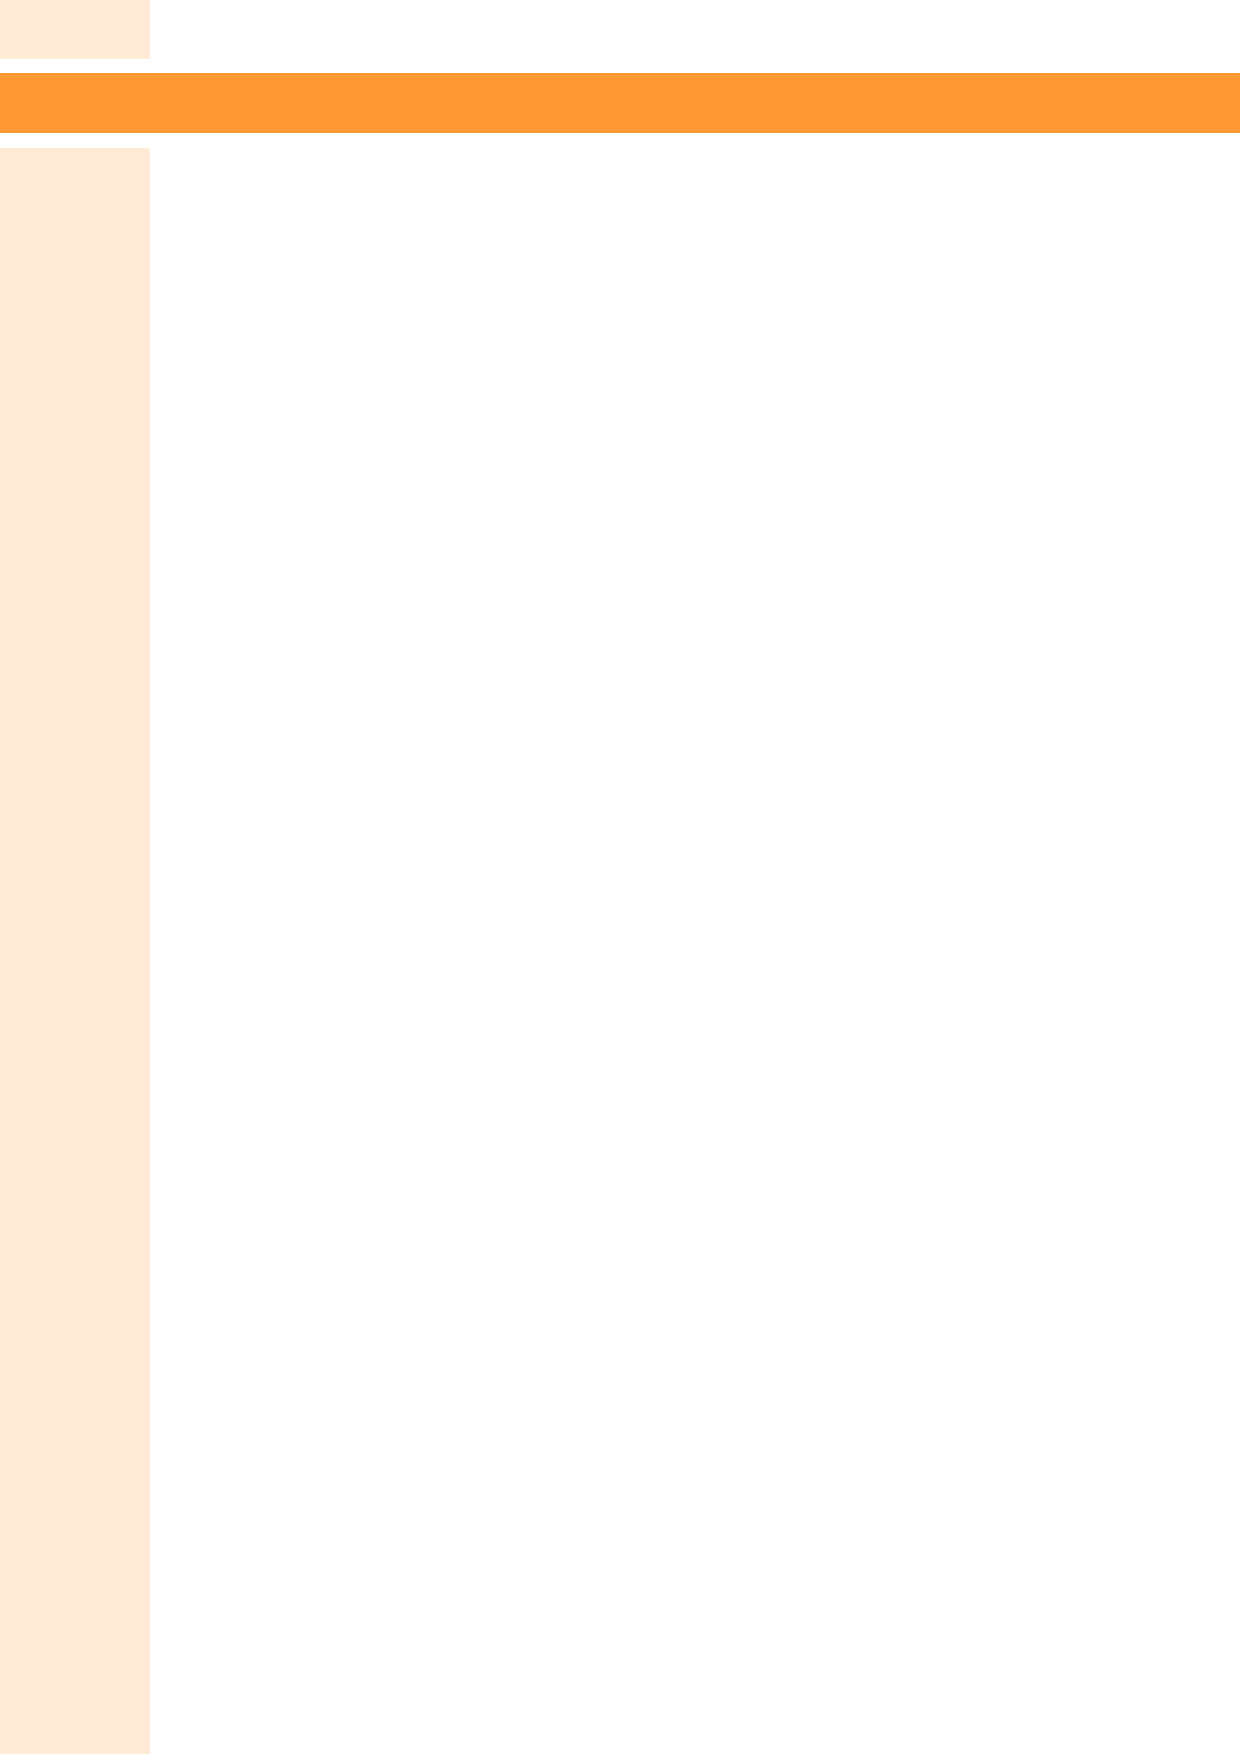
\includegraphics[scale=1]{Cover/cover_background}},
%   }
% \BgThispage

% Decrease the inner margin
\newlength{\savedoddsidemargin}
\setlength{\savedoddsidemargin}{\oddsidemargin}
\setlength{\oddsidemargin}{1in}


{\sffamily\setlength{\baselineskip}{9mm}
~
\vfill

{
\LARGE\bfseries
\titlestring
}

\vspace{0.5in}

{\Large
Romain Jacob
}

\vspace{0.8in}

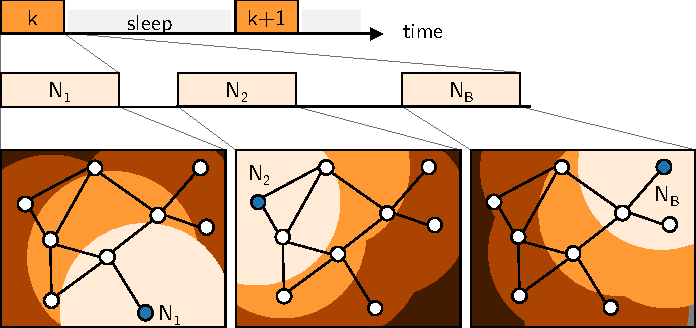
\includegraphics[scale=1]{Cover/cover_image}

\vspace{0.8in}

{\Large
Diss.\ ETH No.\ \dissnumstring
}

}

\clearpage

%Restore the initial values
\setlength{\oddsidemargin}{\savedoddsidemargin}

\clearpage

\firstpagefalse % For background image

\newcommand{\dissnumstring}{XX}
\newcommand{\titlestring}{XX}
\newcommand{\titlestringNOBR}{%
Leveraging Synchronous Transmissions for the Design of Real-time Wireless Cyber-Physical Systems
%
}

\newcommand{\degreestring}{Doctor of Sciences of ETH Zurich}
\newcommand{\degreestringabr}{(Dr. sc. ETH Zurich)}
\newcommand{\authorstring}{Romain Jacob}
\newcommand{\acatitlestring}{M.Sc. École Normale Supérieure de Cachan}
\newcommand{\dateofbirthstring}{03.12.1990}
\newcommand{\citizenstringA}{France}
\newcommand{\examinerstring}{Prof. Dr. Lothar Thiele}
\newcommand{\coexaminerstringA}{Prof. Dr. Thiemo Voigt}
\newcommand{\coexaminerstringB}{Prof. Dr. Martina Maggio}
\newcommand{\datestring}{November 2019}

\begin{titlepage}
{
\sffamily\setlength{\baselineskip}{10mm}

\begin{centerline}
{\large\noindent Diss.\ ETH No.\ \dissnumstring}
\end{centerline}
\vfill

\begin{center}
\LARGE\bfseries
\titlestringNOBR
\end{center}
%\vspace{1mm}
\vfill

\begin{center}
\large A thesis submitted to attain the degree of
\end{center}
\vspace{0.55\fill}

\begin{center}
\large \degreestring \linebreak \degreestringabr
\end{center}
\vspace{0.55\fill}

\begin{center}
\large presented by \linebreak \authorstring %\linebreak \acatitlestring
\linebreak \linebreak born on \dateofbirthstring \linebreak citizen of
% \linebreak
\citizenstringA
\end{center}
\vspace{3\fill}

\begin{center}
% \large accepted on the recommendation of \linebreak
\large submitted to \linebreak
\examinerstring, examiner \linebreak
\coexaminerstringA, co-examiner \linebreak
\coexaminerstringB, co-examiner
\end{center}
\vspace{0.55\fill}

\begin{center}
\large{\datestring}
\end{center}
}
\end{titlepage}

\cleardoublepage
% !TEX root = 00_thesis.tex

\thispagestyle{empty}
\noindent
\includegraphics[scale=.6]{tik}
\medskip
\hrule
\begin{flushright}
\vspace{0.5cm}
TIK-SCHRIFTENREIHE NR. 181
\\ \vspace{1cm}
\large Romain Jacob \\ \vspace{1cm}
\end{flushright}
\begin{flushright}
\Large\bfseries
\titlestring
\end{flushright}
\vspace{\fill}
\hrule
\bigskip

\includegraphics[scale=0.7]{eth}


\clearpage
\thispagestyle{empty}


\noindent
A dissertation submitted to ETH Zurich\\
for the degree of Doctor of Sciences

\noindent DISS.\ ETH NO.\ \dissnumstring

\noindent \examinerstring, examiner\\
\coexaminerstringA, co-examiner\\
\coexaminerstringB, co-examiner

\noindent Examination date: December 17, 2019\\
\vfill
\noindent
%ISBN XXX-XXXXXXXXXX\\
%DOI \href{http://dx.doi.org/XX.XXXX/ethz-a-XXXXXXXXX}{XX.XXXX/ethz-a-XXXXXXXXX}


\cleardoublepage
\chapter*{}
\vfill
{%\footnotesize
\begin{flushright}
\emph{À mes parents, qui m'ont permi de devenir ce que je suis aujourd'hui.\\
À ma femme, qui m'aide à devenir meilleur chaque jour.}
\end{flushright}
}
\vfill

\cleardoublepage
\frontmatter
\pagestyle{headings}
% !TEX root = 00_thesis.tex
\chapter[Abstract]{Abstract}

% Context
%% CPS
\startsquarepar
Cyber-Physical Systems (\CPS) refer to systems where some intelligence is embedded into devices that interact with their environment; that is, collecting information from the physical space, processing that information, and taking actions that affect the environment. Automatically turning the heating on when room temperature gets cold is one of the simplest example of \CPS.\linebreak
%
Things get more complex when applications are distributed between low-power devices that should operate autonomously for multiple years. Then, performing reliable and energy efficient wireless communication becomes paramount.
%
Moreover, applications often specify deadlines; that is, maximal tolerable delays between the execution of distributed tasks.
Systems that guarantee to meet such deadlines are called real-time systems.
%
Wireless \CPS capable of providing real-time guarantees while using low-power communication technology are desirable but they are particularly challenging to design.
%% ST
In the past few years, a technique known as synchronous transmissions (\ST) has been shown to enable reliable and energy efficient communication in low-power multi-hop networks.
\linebreak
In a nutshell, \ST consists in letting multiple devices transmit a packet during the same time interval; communication is likely to be successful if the transmissions are well synchronized, hence the name of \emph{synchronous} transmissions.
\ST can be leveraged to realize any multi-hop broadcast --~a one-to-all communication~-- in a given time; a very interesting property for designing real-time systems.
\stopsquarepar

% Need: what you have vs. what you want
While the potential of \ST is recognized by the low-power wireless academic community, this technique has not yet been leveraged for the design of \CPS.\linebreak
We identify at least three issues that limit the adoption of \ST in this domain:
\linebreak
\smallBox{(i)}\ST is difficult to use due to stringent time synchronization requirements: in the order of \us.
There is a lack of tools to facilitate the implementation of \ST by \CPS engineers, which are often not wireless communication experts.
\linebreak
\smallBox{(ii)}There are only few examples showcasing the use of \ST for \CPS applications and academic works based on \ST tend to focus on communication rather than applications. Convincing proof-of-concept \CPS applications are missing.
\linebreak
\smallBox{(iii)}The inherent variability of the wireless environment makes performance evaluation challenging. The lack of an agreed-upon methodology hinders experiment reproduciblility and limits the confidence in the performance claims.

% task
Consequently, we developed support tools and methods to facilitate the evaluation of wireless protocols and the implementation of \CPS based on \ST.
\linebreak
Furthermore, we leveraged \ST to design two \CPS solutions targeting different classes of real-time applications.
% object
This dissertation presents these contributions.

\begin{itemize}

  % =============================== %
  \item
  \startsquarepar
  In \cref{ch:triscale}, we propose to design and analyze performance evaluation experiments for networking protocols using a concrete, rational, and statistically sound methodology.
  We implement this methodology in a framework called \triscale  which allows to make performance claims with quantifiable levels of confidence.
  Furthermore, we leverage the \triscale framework to propose the first formalized definition of reproducibility for networking experiments.
  \stopsquarepar

  % =============================== %
  \item
  \startsquarepar
  \cref{ch:baloo} presents \baloo, a flexible design framework for network stacks based on \ST.
  Users implement their protocol through the programming interface offered by \baloo while the framework handles the complex low-level operations; \eg meeting the time synchronization requirements of \ST.
  \linebreak
  We show that \baloo is flexible enough to implement a wide variety of communication protocols while introducing only limited memory and energy overhead.
  \stopsquarepar

  % =============================== %
  \item
  Finally, we design and implement two wireless \CPS based on \ST:
  {\setlength{\parskip}{0pt}%
    \begin{itemize}[nosep]
      \item the Distributed Real-time Protocol (\DRP) uses contracts to maximize the flexibility of execution between distributed tasks~(\cref{ch:drp});
      \item Time-Triggered Wireless (\TTW) statically co-schedules all task executions and packet transfers to minimize end-to-end latency~(\cref{ch:ttw}).
    \end{itemize}
    \startsquarepar
    % Findings
    We demonstrate that real-time guarantees can be provided in a reliable and energy efficient manner.
    Furthermore, \TTW supports update rates of tens of \ms, which is sufficient to perform distributed closed-loop control of inverted pendulums -- a fundamental benchmark for control and robotic applications.
    \stopsquarepar
  }

\end{itemize}

% Conclusion
\startsquarepar
With this dissertation, we showcase that \ST is suitable to meet the requirements of real-time wireless \CPS. Furthermore, we facilitate the implementation of such systems with \baloo, a design framework that makes \ST accessible to the non-expert. Finally, \triscale provides an important building block to confidently evaluate the performance of networking protocols -- an essential building block of wireless \CPS.
% Perspectives
Building on \triscale, it would be useful to define benchmark problems representative of different classes of applications to serve as baseline for the evaluation of future wireless \CPS solutions. Ultimately, we must transition from proof-of-concepts to real-world wireless \CPS applications; this would be further facilitated by porting \baloo to newer and more powerful platforms, thereby pushing the limits of achievable performance levels.
\stopsquarepar

% !TEX root = 00_thesis.tex
\chapter{Résumé}

% Context
%% CPS
\startsquarepar
Les systèmes cyber-physiques (\CPS, de l'anglais \emph{Cyber-Physical Systems}) sont des systèmes où des éléments informatiques interagissent avec leur environnement : ils collectent certaines informations sur leur environnement, traitent ces informations et agissent en conséquence, ce qui modifie l'état de l'environnement.
Monter automatiquement le chauffage lorsque la température baisse est l'un des exemples les plus simples de \CPS.
%
La situation devient plus complexe lorsque les applications sont distribuées entre des systèmes embarqués à
faible consommation d'énergie, qui sont supposés fonctionner de façon autonome durant plusieurs années.
Une communication sans-fil fiable et à basse consommation devient alors essentielle.
%
De plus, des délais maximum sur l'exécution de différentes opérations sont souvent imposés. Un système capable de garantir ces délais est appelé un système temps-réel.
%
Des \CPS sans-fil  capablent de fournir des garanties temps-réel tout en utilisant des technologies de communication à basse consommation sont souhaitables mais difficiles à concevoir.
%% ST
Ces dernières années, une technique appelée transmission synchrone (\ST, de l'anglais \emph{synchronous transmissions}) a été utilisée pour communiquer de façon fiable et à basse consommation dans les réseaux multi-sauts.
\linebreak
En un mot, le principe de la \ST est d'autoriser différents appareils à transmettre un paquet durant le même intervalle de temps ; la communication a de bonnes chances de réussir si les transmissions sont suffisamment bien synchronisées.
La \ST peut être utilisée pour réaliser en un temps donné n'importe quel broadcast multi-saut, \cad une communication depuis un appareil à tous les autres ; une propriété très intéressante pour concevoir un système temps-réel.
\stopsquarepar

\startsquarepar
Bien que le potentiel de la \ST soit reconnu par la communauté académique réseaux, cette technique a été pour l'instant peu utilisée pour la conception de \CPS.
Au moins trois problèmes limitent l'adoption de la \ST dans ce domaine.
\linebreak
\smallBox{(i)}La \ST est difficile à utiliser à cause des exigences strictes de synchronisation, de l'ordre de la \us.
Il manque des outils facilitant l'usage de la \ST par des ingénieurs \CPS, qui souvent ne sont pas des experts en communication.
\linebreak
% \\
\smallBox{(i)}Il y a peu d'exemples illustrant l'utilisation de la \ST pour des applications \CPS ; les travaux académiques sur la \ST sont souvent plus focalisés sur les aspects communication que application.
Il manque de preuves de concept convaincantes démontrant l'intérêt de la \ST pour des applications \CPS.
% There are only few examples showcasing the use of \ST for \CPS applications and academic works based on \ST tend to focus on communication rather than applications. Convincing proof-of-concept \CPS applications are missing.
\linebreak
\smallBox{(i)}La variabilité inhérente de l'environnement sans-fil rend difficile l'évaluation des performances. L'absence d'une méthode établie menace la reproductibilité des expériences et limite la confiance dans les performances annoncées.
\stopsquarepar

\pagebreak
\startsquarepar
Ainsi, nous avons développé des outils et méthodes pour faciliter l'évaluation de protocoles sans-fil et l'implémentation de \CPS utilisant la \ST.
De plus, nous avons tiré parti de la \ST pour concevoir deux \CPS visant différentes classes d'applications temps-réel.
Cette dissertation présente ces contributions.
\stopsquarepar

\begin{itemize}

  % =============================== %
  \item
  \startsquarepar
  Dans le chapitre \ref{ch:triscale}, nous proposons de concevoir et d'analyser les expériences d'évaluation de performance pour les protocoles réseaux en utilisant une méthodologie concrète, rationnelle et statistiquement robuste.
  Nous implémentons cette méthodologie dans un framework appelé \triscale, qui permet d'obtenir des performances avec un niveau de confiance quantifiable.
  % \linebreak
  De plus, nous tirons parti de \triscale pour proposer la première définition formelle de reproductibilité appliquée aux expériences pour les protocoles réseaux.
  \stopsquarepar

  % =============================== %
  \item
  % \startsquarepar
  Le chapitre \ref{ch:baloo} présente \baloo, un framework pour la conception de protocoles réseaux basés sur la \ST.
  L'utilisateur implémente son protocole via l'interface fournie par \baloo, qui prend en charge la gestion des opérations complexes telles que garantir la synchronisation nécessaire pour la \ST.
  Nous montrons que \baloo est suffisamment flexible pour implémenter un large panel de protocoles pour un coût minime en termes d'utilisation mémoire et de consommation d'énergie.
  % \stopsquarepar

  % =============================== %
  \item
  Enfin, nous concevons et implémentons deux \CPS sans-fil utilisant la \ST :
  {\setlength{\parskip}{0pt}%
    \begin{itemize}[nosep]
      \item
      le Distributed Real-time Protocol (\DRP) utilise le concept de contrat pour maximiser la flexibilité entre les tâches à exécuter~(Chapitre~\ref{ch:drp}) ;
      \item
      Time-Triggered Wireless (\TTW) planifie statiquement tous les échanges de paquets et les exécutions de tâches de façon à minimiser la latence de bout en bout entre les tâches~(Chapitre~\ref{ch:ttw}).
    \end{itemize}
    \startsquarepar
    Nous démontrons que des garanties temps-réel peuvent être fournies de façon fiable et efficace en énergie.
    De plus, \TTW supporte des latences de l'ordre de dizaines de \ms, ce qui est suffisant pour contrôler en boucle fermée des pendules inversés ; une référence pour les applications de contrôle et de robotique.
    \stopsquarepar
  }

\end{itemize}

% Conclusion
\startsquarepar
Dans cette dissertation, nous montrons que la \ST permet de satisfaire les exigences des \CPS sans-fil temps-réel.
De plus, nous facilitons l'implémentation de tels systèmes avec \baloo, un framework qui rend la \ST accessible pour le non-expert.
Enfin, \triscale est un élément important pour améliorer la confiance dans les performances des protocoles réseaux.
À partir de \triscale, il serait utile de définir, pour différentes classes d'applications, des problèmes de références pour l'évaluation de futurs \CPS.
In fine, il est nécessaire d'évoluer depuis les preuves de concept vers des applications de \CPS sans-fil dans le monde réel. Cela serait facilité par le portage de \baloo sur des systèmes embarqués plus récents et plus puissants, ce qui améliorerait les performances atteignables.
\stopsquarepar


\cleardoublepage
\chapter[Acknowledgments]{Acknowledgments}


\clearpage
\pagestyle{empty}
\pdfbookmark[0]{Table of Contents}{Table of Contents}
{\small\tableofcontents}
\cleardoublepage
%\phantomsection\addcontentsline{toc}{chapter}{List of Figures}
%\listoffigures
%\cleardoublepage
%\phantomsection\addcontentsline{toc}{chapter}{List of Tables}
%\listoftables
%\cleardoublepage

\mainmatter
\pagenumbering{arabic}
\setcounter{page}{1}
\pagestyle{headings}
%

\TODO{
\begin{itemize}
  % \item CRediT for each chapter! -> Nope, give it up for now
  \item `click` message on hover (pdf)
\end{itemize}
}

% !TEX root = 00_thesis.tex

\chapter{Introduction}
\label{ch:introduction}

\TODO{
\begin{itemize}
	\item Fig4: left-align. remove white boxes
\end{itemize}
}


Cyber-Physical Systems (\CPS) are understood as systems where ``\emph{physical and software components are deeply intertwined, each operating on different spatial and temporal scales, exhibiting multiple and distinct behavioral modalities, and interacting with each other in a myriad of ways that change with context}''~\cite{nsf2010Cyber}.
The domains of application of \CPS are very diverse: \eg robotics, distributed monitoring, process control, power-grid management~\cite{stankovic2008WSAN, lee2008Cyber, rajkumar2010CPS}.

It is important to realize that the design of \CPS encompasses three main aspects, mapping to as many research fields, with their own purpose and goals: %\linebreak
% \begin{itemize}
	% \inlineitem
	The \emph{embedded hardware design} aims to extend the amount of computational resources available (\eg processing power, memory, sensors and actuators) while limiting the cost, form factor, and energy consumption of a device.
	% \linebreak
	% \inlineitem
	The \emph{communication}, either wired or wireless, aims to transmit messages between distributed devices efficiently; that is, quickly and using little energy.
	% \linebreak
	% \inlineitem
	Finally, the \emph{distributed system design} realizes the implementation of the \CPS functions, such as \eg remote monitoring and control of distributed processes.
% \end{itemize}

The goal of the overall design is to reliably provide the specified \CPS functions.
Achieving this goal relies on hardware and communication; however reaching ``perfect'' communication, such as 100\% packet reception rate, is not a goal in itself; it is merely a mean to an end. What truly matters is to fulfill the system functionality.
Typically, \CPS design aims to provide end-to-end performance guarantees, such as meeting hard deadlines between the execution of distributed tasks; for example, between the start of a sensing task to the end of the corresponding actuation tasks -- \cref{fig:e2ePerf}.
Meeting such deadlines is called \emph{providing real-time guarantees}.

\begin{figure}
  \centering
  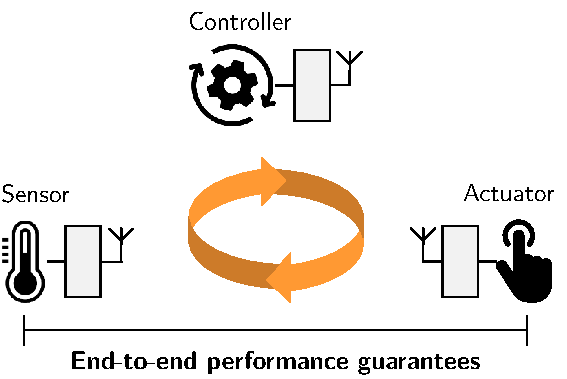
\includegraphics[scale=1]{e2ePerformance}
  \caption{The primer objective of \CPS design is to provide end-to-end performance guarantees for distributed applications.
	{In this dissertation, we consider synchronous transmissions, a recent development in low-power wireless communication, and attempt to leverage the technique to provide real-time guarantees in wireless \CPS.}}
  \label{fig:e2ePerf}
\end{figure}

The potential benefits of wireless communication for \CPS applications are well-known and include \eg simpler deployment and maintenance, cheaper operational costs, lighter weight~\cite{luvisotto2017Ultra}.
Furthermore, wireless is the only viable option in application domains including highly mobile nodes, such as an automated warehouse with transport robots~\cite{haegele2018Logistics} or teams of drones~\cite{mottola2014Teamlevela}.
However, \CPS applications have challenging performance requirements~\cite{akerberg2011Future}, which are hard to fulfill with a wireless design.


\section{Requirements of Wireless \CPS}

\CPS applications are subject to different types of requirements, such as the specified end-to-end latency, bandwidth, or number of devices; the precise performance level for these requirements depends on the application context.
Generally, \CPS requirements belong to one of the following classes:

\begin{features}[labelwidth=65pt, leftmargin=(\labelwidth+\labelsep)]

  \item[Reliability]
  A large ratio of messages are successfully transmitted wirelessly.

  \item[Adaptability]
  The system adapts to runtime changes in resource demands.

	\item[Mobility]
  The system supports mobile devices.

	\item[Timeliness]
  Applications meet their deadlines, which are often specified end-to-end. Depending on the class of systems, deadlines can be either soft or hard~\cite{buttazzo2011HardRT}.

  \item[Efficiency]
  The system
  supports short end-to-end latency,
  scales in terms of system size,
  and
  optimizes its energy consumption and bandwidth utilization.

\end{features}

These requirements are mutually conflicting. For example, reducing the energy consumption is typically achieved by keeping the radio turned off whenever possible.
However, this directly conflicts with \feature{Adaptability}, as the system cannot adapt reliably without exchanging some extra messages.
In general, there is a price to pay in terms of \feature{Efficiency} for meeting any of the other requirements.
Hence, designing \CPS consists in exploring the design space for relevant trade-offs; that is, the design optimizes the overall system \feature{Efficiency} while meeting other application requirements.



\section{Traditional Wireless Networking}
\label{sec:traditionalNetworking}

Low-power wireless communication is a mature field of research, heavily studied for more than two decades.
A large part of the research focused on wireless sensor networks, where low power consumption is a key requirement to enable long-term operation of the deployed networks, with specifications up to multiple years of operation on small batteries.
Many successful applications and deployments include monitoring of soils~\cite{geissdoerfer2019PREAct}, permafrost~\cite{weber2019decade}, buildings~\cite{chintalapudi2006Monitoring}, or wildlife~\cite{cassens2019Bursting, zhang2004Zebranet}.

In these scenarios, the distributed application often remains simple (\eg collect sensor readings).
The main challenge is to reliably aggregate or disseminate messages across a multi-hop network.
\emph{Single-hop} communication refers to the case where a source node is in communication range from its destination. This is a rather simple case, but the deployed networks often span large areas whereas low-power radios can typically communicate in the range of tens of meters.
Thus, \emph{multi-hop} communication is required, whereby a source node must rely on other nodes in the network to forward its messages, hop after hop, until the destination is reached.%
%
% \footnote
{This is the same principle as in the children's game known as Chinese whispers~\cite{ChineseWhispers}; if you ever played, you know that the original message hardly ever reaches the end of the chain successfully.}
%

Multi-hop communication is a collaborative task for which the nodes must be coordinated.
Indeed, if a node transmits a message while another wireless communication is ongoing, the transmissions will interfere and they may both fail.
% This is a key difference between wired and wireless communication: In a wired network, when a packet arrives at a switch or a router for forwarding, it can be en-queued and transmitted later; With wireless communication, packets are lost and must be retransmitted.
Furthermore, the radio frequency bands used for wireless communication cannot be isolated. Other networks are potentially exchanging messages on the same frequencies, which generates external interference and triggers packet losses.
As a result, traditional multi-hop communication requires complex mechanisms for coordinating the nodes, scheduling the different transmissions to forward all messages throughout the network, and retransmitting messages that have been lost (\eg due to external interference).
The complexity is further increased in mobile scenarios, where the set of neighboring nodes (which may relay a node's messages) changes frequently.
%
The traditional wireless networking approach performs multi-hop communication by carefully planning a sequence of unicasts (\ie one-hop transmissions), usually performed along one or a few of the shortest paths possible between a message source and its destination~\cite{watteyne2016Industrial,kim2017Challenging, mottola2011MUSTER}.
Intuitively, this is efficient because only the necessary nodes are involved in relaying a message.

In practice however, multi-hop wireless network are sensitive to topology changes, external interference, and traffic congestion. These limit the reliability of communication, which has been a major obstacle to the utilization of wireless technology in \CPS: for a long time, it has been considered impossible to provide the required level of reliability using wireless~\cite{stankovic2005Opportunities}.
Synchronous transmissions have fundamentally changed that.

\section{Synchronous Transmissions}
\label{sec:ST}

Synchronous transmissions (\ST), also referred to as concurrent transmissions, is a technique consisting in letting  multiple nodes transmit a message at the ``same time'' (hence the name of \emph{synchronous} transmissions).
A destination node can successfully receive (one of these) synchronous transmissions thanks to two effects taking place at the physical layer: constructive interference and the capture effect~\cite{yuan2013LetTalkTogether, escobar-molero2019Improving}.
In a nutshell, \ST is likely to be successful if the incoming messages arrive at the receiving node's antenna within a small time offset (in the range of a few symbol periods -- a few tens of \us~-- depending on the physical layer and the effect considered).
\ST has been shown to work both analytically~\cite{wilhelm2014Reception}, empirically~\cite{ferrari2011Glossy}, and on different physical layers, such as IEEE 802.15.4\cite{yuan2014Sparkle}, Bluetooth~\cite{alnahas2019BlueFlood}, and LoRa~\cite{wegmann2018Reliable}.

The use of \ST in low-power communication, pioneered by Glossy~\cite{ferrari2011Glossy} in 2011, has triggered a paradigm shift in the low-power wireless community: \ST can be leveraged to implement efficient broadcast in a multi-hop network using network-wide flooding~(\cref{fig:flooding}).
The flooding procedure implemented by Glossy is illustrated in \cref{fig:glossy}. A first node initiates the flooding process. The 1-hop neighbors of the initiator receive the message and synchronously broadcast this same message in the next time step, which is then received by the initiator's 2-hop neighbors with high probability, thanks to \ST. The process repeats following the same logic: a node that receives a packet broadcasts it again in the next time slot. Each node in the network transmits each packet up to $N$ times, after which the flood terminates.
It has been shown in a wide range of scenario that, with $N=3$, Glossy achieves a reliability above 99.99\%~\cite{ferrari2011Glossy}; that is, 99.9\% of the floods are successfully received by nodes in the network. With $N=5$, the average reliability reaches 99,999\%~\cite{ferrari2011Glossy}.
Glossy achieves such high reliability by leveraging spatio-temporal redundancy.
Packets are transmitted along all possible paths; in other words, they are implicitly routed everywhere, and therefore avoid interference sources localized in space.
In addition, having each node transmitting $N$ times creates temporal redundancy, thereby avoiding interference sources localized in time.
Moreover, the predictability of the operation timing in \ST-based flooding can be leveraged to perform distributed time synchronization. Glossy demonstrated that sub-\us synchronization accuracy can be achieved in a multi-hop network composed of tens to hundreds of nodes~\cite{ferrari2011Glossy}.
Since Glossy, other flooding strategies have been proposed~\cite{lim2017Competition, baddeley2019AtomicSDN, ma2019DeCoT}, but the overall principle remains the same.

\begin{figure}
  \centering
	\captionsetup[subfigure]{labelformat=empty,justification=centering}
  \begin{subfigure}[t]{0.3\linewidth}
      \centering
      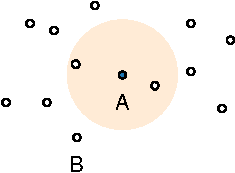
\includegraphics[scale=1]{flood_1}
			\caption{Node \textbf{A} initiates the flood.}
      \label{fig:flooding1}
  \end{subfigure}%
  \hfill
  \begin{subfigure}[t]{0.33\linewidth}
      \centering
      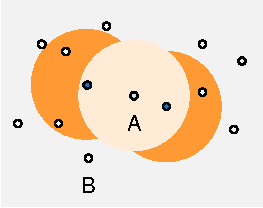
\includegraphics[scale=1]{flood_2}
			\caption{The 1-hop neighbors of \textbf{A} synchronously repeat.}
      \label{fig:flooding2}
  \end{subfigure}%
  \hfill
  \begin{subfigure}[t]{0.33\linewidth}
      \centering
      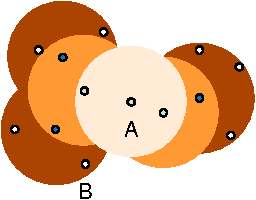
\includegraphics[scale=1]{flood_3}
			\caption{Node \textbf{B} receives the message.}
      \label{fig:flooding3}
  \end{subfigure}
  \caption{%
  Flooding process for a message sent from node \textbf{A} to node \textbf{B}}
  \label{fig:flooding}
\end{figure}

\begin{figure}
  \centering
  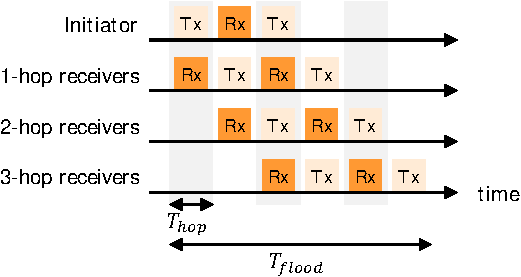
\includegraphics[scale=1]{glossy}
  \caption{Glossy operation in a 3-hop network with 2 transmissions per node ($N$)}
  \label{fig:glossy}
	\vspace{-0.2cm}
\end{figure}


The key benefit of \ST is that, thanks to the provided multi-hop broadcast primitive, the overall communication design can be dramatically simplified.
Essentially, one can abstract the underlying multi-hop topology as a \emph{virtual single-hop network}, which can scheduled like a shared bus: any node can send a message to any other node(s) in the network in bounded time. The only requirement is that no other node is using the ``bus'' at the same time.
This design, first proposed with the Low-power Wireless Bus protocol~\cite{ferrari2012LWB}, has been adapted into many different flavors~(\eg \cite{istomin2018Interferenceresilient, alnahas2017a2, sarkar2016Sleeping, baddeley2019AtomicSDN}) with always a similar concept~(\cref{fig:rounds}): communication is organized in rounds, between which nodes keep their radio turned off to save energy. Each round is composed of time slots, which are assigned to certain nodes for communication. In each of these slots, nodes execute a flooding primitive (\eg Glossy) thereby preforming a one-to-all communication.
Consequently, the complexity of performing reliable multi-hop communication (described in \cref{sec:traditionalNetworking}) is significantly relaxed.
Thanks to \ST, multi-hop communication is reduced to the scheduling of a single shared resource, a well-understood and relatively easy problem~\cite{buttazzo2011HardRT}.

\begin{figure}
  \centering
  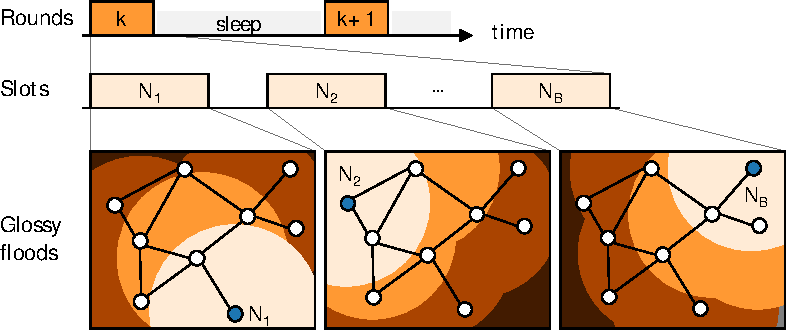
\includegraphics[scale=1]{rounds}
  \caption{Thanks to synchronous-transmissions based flooding, a multi-hop network can be abstracted and scheduled like a shared bus.
	Communication is organized in rounds, composed of time slots; in each time slot, a node initiates a flood which allows to send a message to any other node(s) in bounded time.\linebreak
	This mimics the operation of classical field bus, but with a wireless design.}
  \label{fig:rounds}
	\vspace{-0.5cm}
\end{figure}

A priori, flooding seems to be a wasteful approach: every message sent by any node will be received and forwarded by every other node in the network.
However, the simplicity and reliability of the approach actually pays off.
\linebreak
% \inlineitem
(i)~Since~the flooding logic is simple, it requires little communication overhead for the coordination of the network; nodes mostly send application data.
% \linebreak
% \inlineitem
(ii)~The~spatio-temporal redundancy embedded in the flooding process makes it very reliable; once a flood is completed, there is hardly ever a need to further retransmit a message in a subsequent flood.
% \linebreak
% \inlineitem
(iii)~Finally, since multiple nodes can transmit simultaneously, the flooding process completes quickly; very close to the theoretically optimal speed~\cite{ferrari2011Glossy}.

Thus, with flooding approaches based on \ST, the energy cost of sending one byte of data is relatively high (since this byte will be retransmitted by all the nodes), but the \emph{overall cost} for communication remains relatively small, thanks to the limited protocol overhead and the absence of need for further retransmissions.
The energy efficiency and reliability of \ST-based flooding has been demonstrated in many research contributions~(\eg \cite{ferrari2011Glossy, landsiedel2013Chaos, herrmann2018Mixer}) and showcased in the EWSN Dependability Competitions~\cite{schuss2017Competition}, where all wining solutions in the past four years (2016 to 2019) were based on \ST~\cite{escobar2018Competition, sommer2016Competition,lim2017Competition, escobar2019RedNodeBus, ma2019DeCoT}.


The downside of \ST is that it is difficult to use in more complex system designs, such as those envisioned for wireless \CPS~\cite{akerberg2011Future}.
The difficulty stems from the tight timing requirements for successful \ST: to be received reliably, transmissions must be initiated by the different nodes within few \us.
Practically, this implies that the runtime execution of a node is governed by the communication protocol, which makes the implementation of advanced distributed tasks complex and error prone.
As a consequence, \ST has thus far been mainly used for academic endeavors and mostly in wireless sensor network scenarios where the application tasks are typically simple and non-critical.
Collecting a new sensor reading is a task that can usually tolerate being delayed by a few milliseconds while communication is ongoing.\linebreak
This is generally not acceptable for wireless \CPS.

% ------------------------------------------------------------------------------
\section{The Dual-Processor Platform}
\label{sec:dpp}

In \CPS, each device must perform application and communication tasks in order to fulfill the overall system functions; this poses the challenge of interference between tasks which contend for processor execution time.
This interference problem can be mitigated by a new breed of embedded platforms featuring multiple processing cores, such as the NXP LPC541XX~\cite{nxpLPC541XX} or the VF3xxR~\cite{nxpVF3xxR}.
On the one hand, this helps because applications and communication tasks can be processed in parallel, but on the other hand, it creates contention for the access to the resources shared between the cores.
Efficient scheduling of multi-core platforms is a complex problem and a research field of its own.


Instead of resolving contention by scheduling, another approach proposed in the literature attempts to \emph{prevent interference by design}. This principle, soberly called the Dual-Processor Platform~(\DPP~-- \cite{beutel2019DPPdemo}), consists in linking two processors with a processor interconnect called \bolt~(\cref{fig:dpp}).
\bolt~\cite{sutton2015Bolt} provides predictable asynchronous message passing between two arbitrary processors while decoupling these processors with respect to time, power, and clock domains.
The lower part of \cref{fig:dpp} shows a conceptual view of the \DPP, including two message queues with first-in-first-out (FIFO) semantics, one for each direction, which are the only communication channels between the interconnected processors.
The guiding principle of \bolt design is to limit the interference between the interconnected processors as much as possible, then to provide formally verified bounds on the unavoidable interference remaining.
Concretely, this means that the \bolt API functions, used by the processors to exchange messages, have hard latency bounds.
The upper part of \cref{fig:dpp} shows an early prototype of a \DPP.
\cref{append:dpp} illustrates other \DPP designs, integrating the concept into smaller form factors and using different processors and targeting different application scenarios.



\begin{figure}
  \centering
  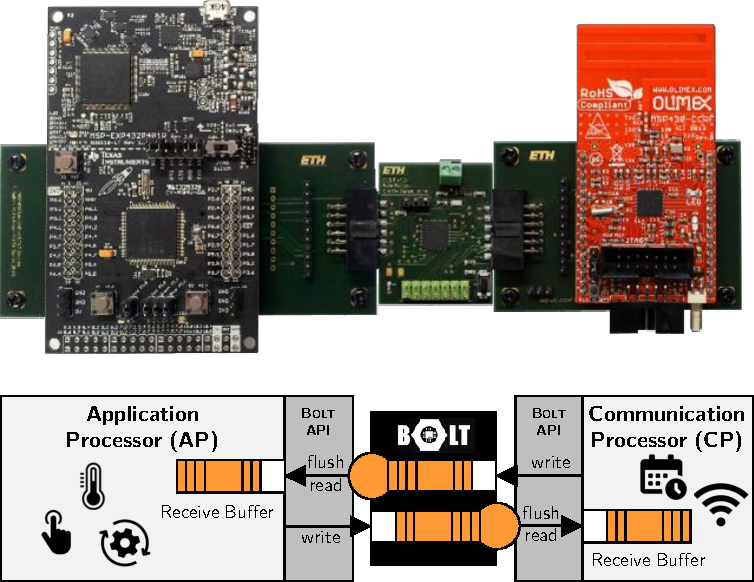
\includegraphics[scale=1]{dpp_with_pic}
  \caption{
    Top: Example of a custom-built heterogeneous \DPP.
		\capt{\bolt (in the middle) interconnects a powerful application processor (TI MSP432~\cite{msp432}) on the left with a state-of-the-art communication processor (TI CC430~\cite{CC430F6137}) on the right.}\linebreak
		%
		Bottom: Conceptual view of the \bolt processor interconnect.
		\capt{Using the \bolt's API functions (\opwrite, \opread, and \opflush), the processors dedicated to application (\AP) and communication (\CP) can asynchronously exchange messages with predictable latency, while otherwise executing independently from one another.}}
  \label{fig:dpp}
\end{figure}


The \DPP concept provides a predictable architecture for wireless \CPS nodes.
By entirely dedicating one processor to the application tasks and another one to wireless communication, we can decouple the timing of communication from the timing of the applications, and therefore facilitate the integration of \ST in a \CPS design.
Furthermore, this helps optimizing performance: each processor can be customized for the specific operations it has to perform. The division of labor fosters specialization, thereby reducing the overall energy consumption and execution time; \ie maximizing \feature{Efficiency}.

% ------------------------------------------------------------------------------
\section{Performance Evaluation in Networking}

Over the past decade, low-power wireless communication has made significant progress, which are not limited to \ST.
The overall level of performance has increased, and it is now common to see reports of packet reception rates above 99\%~\cite{ferrari2011Glossy, duquennoy2015Orchestra, duquennoy2017FiveNines, istomin2018Interferenceresilient}.

The more extreme the performance level, the more critical it becomes to confidently assess the performance.
Higher levels of confidence become necessary to argue about the differences in protocol design and quantify their performance trade-offs.
Obviously, this is import for science as it allow to compare competing approaches.
But it is also important for industry: these new and promising technologies will never be adopted unless we can back our performance claims confidently.
In other words, others must be able to reproduce our experiments.

In the context of wireless networking, reproducible performance evaluation is made particularly challenging by the inherent variability of the experimental conditions: the uncontrollable dynamics of real-world networks~\cite{matos18reproducible, burchfield09rfjungle} and the unsteady performance of hardware and software components~\cite{maricq2018Taming, blackburn2016Truth} can cause a large variability in the experimental conditions, which makes it hard to quantitatively compare different solutions~\cite{bajpai18dagstuhl_report}.

This reproducibility challenge (sometimes even referred to a ``crisis''\cite{baker16reproducibility}) touches all scientific fields, and recently received significant attention in computer science~\cite{collberg15reproducibility, saucez2018Thoughts, bajpai19dagstuhl_guide}.
Yet, how to practically design and execute performance evaluation experiments for wireless protocols remains a largely open question which is being debated by the community~\cite{boano2018IoTBench}.
The lack of a standard for evaluating performance prevents a clear comparison of the different approaches, and therefore hinders the adoption of the technology.

If everyone claims to be the best, it is difficult to trust anyone.

%%%%%%%%%%%%%%%%%%%%%%%%%%%%%%
\pagebreak
\section{Thesis Outline and Contributions}
%%%%%%%%%%%%%%%%%%%%%%%%%%%%%%

\begin{figure}
  \centering
  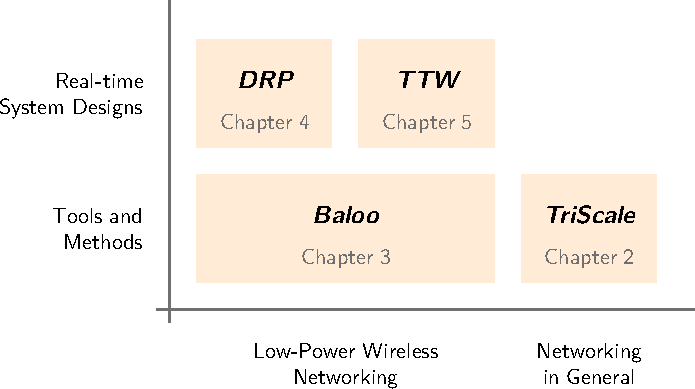
\includegraphics[scale=1]{chapter_all}
  \caption{Overview of the chapters and contributions of this dissertation.}
  \label{fig:chapter_all}
\end{figure}

In this dissertation, we attempt to leverage recent advances in the domain of low-power wireless communication, in particular synchronous transmissions, in order to design wireless \CPS providing end-to-end real-time guarantees.
\cref{fig:chapter_all} provides an overview of the contributions of the dissertation, which are summarized below.
\begin{itemize}

  \item
  We work towards more rigorous and reproducible experimental networking research.
  For the first time, we go beyond simple guidelines and propose a concrete methodology for designing networking experiments and analyzing their data.
  We leverage this methodology to propose the first formalized definition of reproducibility for networking experiments.
  We implemented our methodology in a framework called \triscale, a first-of-its-kind tool that assists researchers by streamlining the design process and automating the data analysis~(\cref{ch:triscale}).

  \item
  We propose and implement \baloo, a design framework for network stacks based on synchronous transmissions (\ST).
  \baloo significantly lowers the entry barrier for harnessing the efficiency, reliability and mobility support of \ST:
  users implement their protocol through a simple yet flexible API while \baloo handles all the complex low-level operations based on the users' inputs~(\cref{ch:baloo}).

  \item
  We demonstrate for the first time that end-to-end real-time guarantees can be obtained in wireless \CPS by leveraging the efficiency and reliability of synchronous transmissions.
  We propose and implement wireless real-time protocols for two different design objectives.
  \begin{itemize}
    \item The Distributed Real-time Protocol (\DRP) uses contracts to maximize the flexibility of execution between application tasks~(\cref{ch:drp}).
    \item Time-Triggered Wireless (\TTW) statically co-schedules all task executions and message transfers to minimize end-to-end latency~(\cref{ch:ttw}).
  \end{itemize}

\end{itemize}



% ------------------------------------------------------------------------------
% Chapter appendices
\begin{subappendices}
% ------------------------------------------------------------------------------

% ------------------------------------------------------------------------------
\newpage
\section{``Reproducible'' Dissertation}

As discussed above, one of the contribution of this dissertation attempts to foster reproducible experimental practices in networking research~(\cref{ch:triscale}).
In line with this idea, we take a step forward in that direction and attempt to make this entire dissertation ``reproducible''.

\begin{itemize}

	\item
	Each chapter includes an ``Artifacts and Links'' appendix. As the name suggests, the reader will find there various links to supplementary materials related to the corresponding chapter.

	\item
	In particular, whenever possible, we make publicly available all the data presented in this dissertation, in both raw and processed form.
	We often provide links to digital notebooks, which allow data visualization in a web browser without requiring any file download.

	\item
	All the plots in this dissertation are ``clickable''; that is, the plots are hyperlinks pointing to dynamic visualizations which let the reader explore the data (\eg zooming-in and -out in the plot, toggle visibility of individual traces, \etc).
	If you are reading a printed version of this document, you can find the corresponding link addresses in the ``Artifacts and Links'' appendices.

	\item
	The source files of this dissertation (this document) are themselves publicly available.
	\tex source files and figures are published on GitHub under the Creative Commons \href{https://creativecommons.org/licenses/by/4.0/}{CC-BY-4.0 license}.

\end{itemize}

% Finally, we must never forget that research is a collaborative endeavor.
% The work presented in this dissertation has been realized with the help of numerous colleagues and dedicated Master students, and we believe it is important to transparently credit each person for their respective contributions.
%
% We do this by using CRediT (Contributor Roles Taxonomy)~\cite{credit}, a standardized taxonomy developed and supported by CASRAI.
% CRediT is high-level taxonomy including 14 roles capturing the typical contributions to scientific scholarly outputs.
% For each chapter, we publish a so-called ``Authors Contributions Statement'' which lists the people that have contributed to the work and their respective role(s).
% These statements are available together with the dissertation files.

% ------------------------------------------------------------------------------
\newpage
\section{Dual-Processor Platforms}
\label{append:dpp}

This appendix illustrates various \DPP designs developed by the Computer Engineering Group at ETH Zurich.
These research prototypes implement the \DPP concepts described in \cref{sec:dpp}, using different processors and targeting different application scenarios. Some of these designs are used in the real-world data collection deployments reported \eg in~\cite{weber2019decade,meyer2019IPSN}.

\vspace{1cm}

\begin{figure}[h]
	\centering
	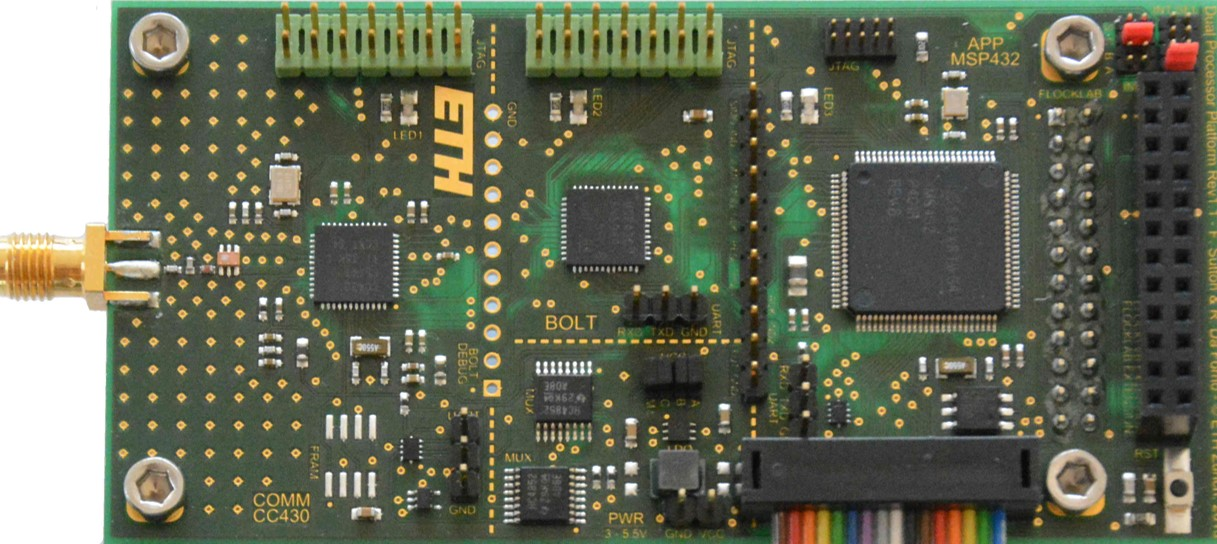
\includegraphics[width=0.8\linewidth]{DPPs/DPP-cc430}
	\caption{Integrated design of the same \DPP as in \cref{fig:dpp}, featuring a TI MSP432~\cite{msp432} as application processor (right) and a TI CC430 SoC~\cite{CC430F6137} as communication processor (left). \bolt sits in the middle, implemented on a TI MSP430 core featuring
64k FRAM~\cite{msp432FR}.}
	\label{fig:dpp-cc430}
\end{figure}

\begin{figure}[!b]
	\centering
	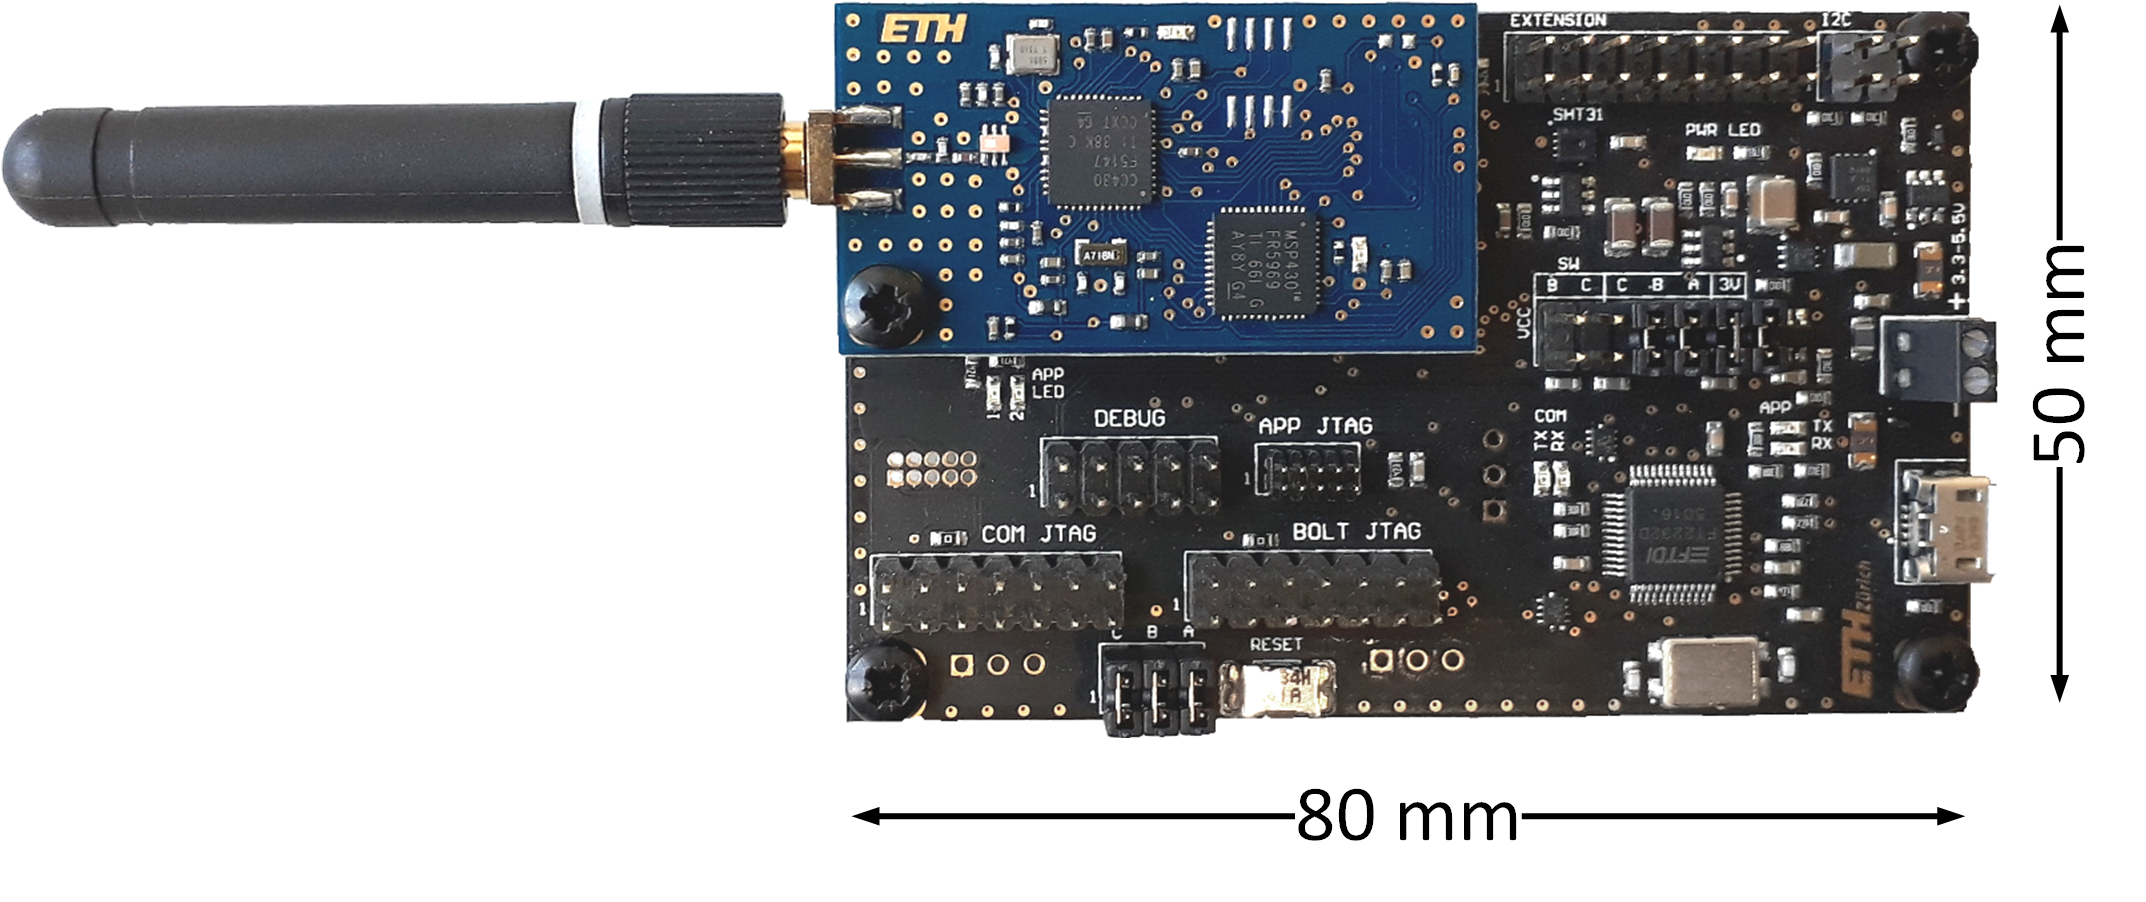
\includegraphics[width=\linewidth]{DPPs/DPP2-cc430}
	\caption{Redesign of the \DPP concept into two separated boards, called the \DPPtwo~\cite{beutel2019DPPdemo}. The lower board (black), called ``application development board'' hosts the application processor (in this case, a TI MSP432~\cite{msp432}) as well as all the I/O, power management, debugging, and other support functions. The upper board (blue) is called the ``communication board'' and hosts the communication processor (in this case, a TI CC430 SoC~\cite{CC430F6137}) and the \bolt interconnect.
	This platform has been used for a prototype wireless \CPS presented in \cite{mager2019Feedback, mager2019Demo} and discussed further in \cref{ch:ttw}.}
	\label{fig:dpp2-cc430}
\end{figure}

\begin{figure}
	\centering
	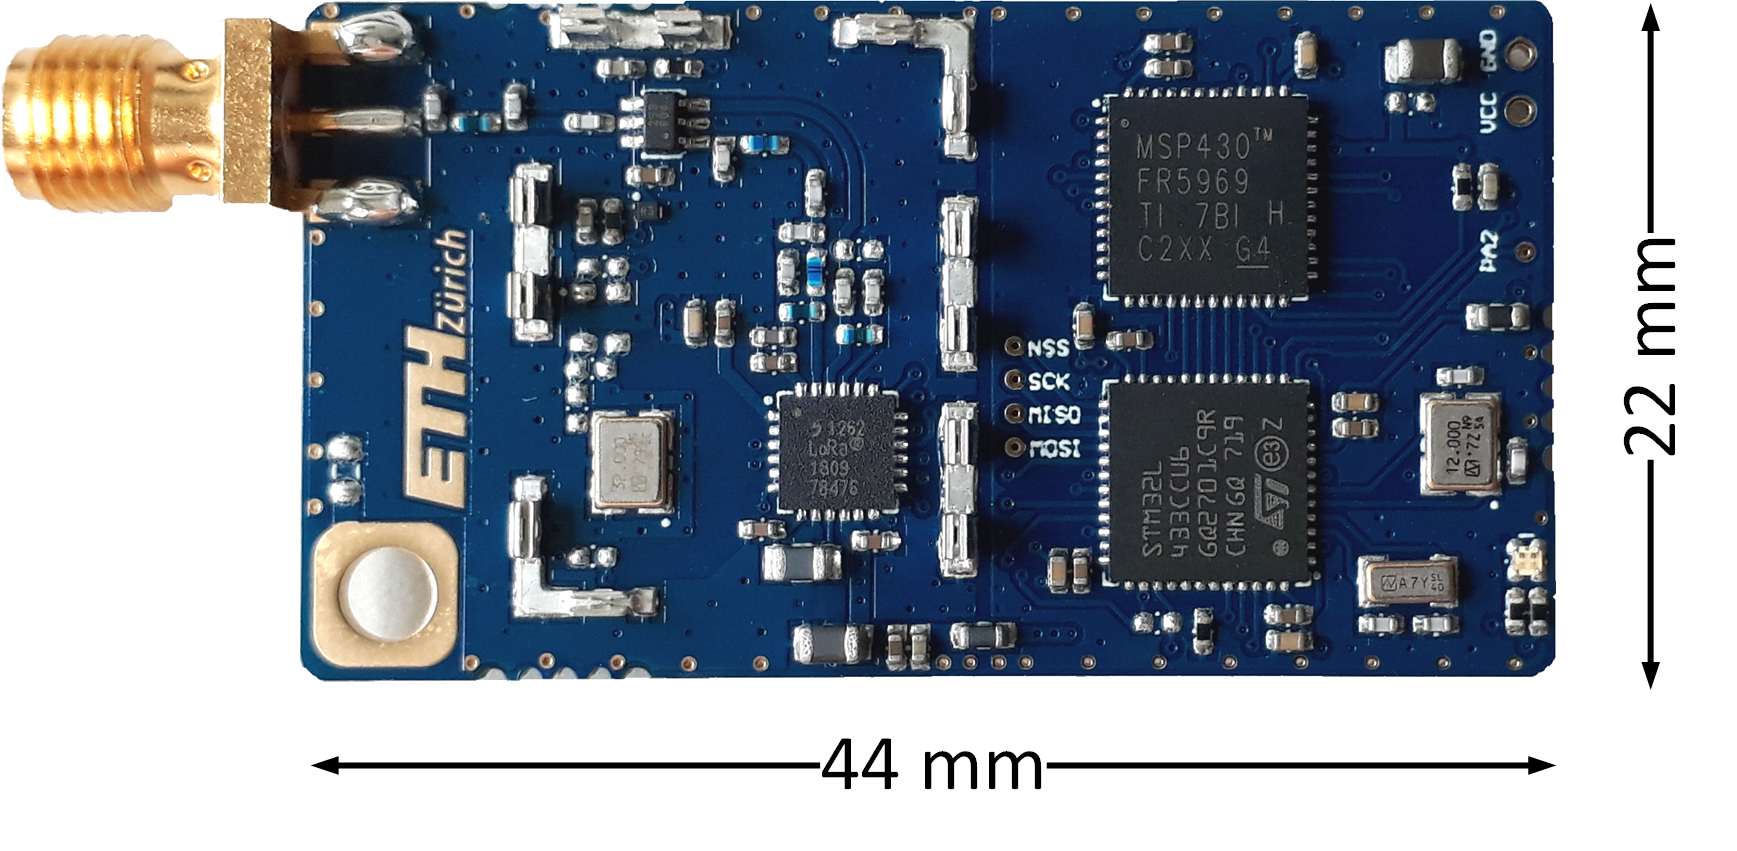
\includegraphics[width=0.8\linewidth]{DPPs/DPP2-LoRa}
	\caption{A different \DPPtwo ``communication board'' featuring a STM32L4 ARM core and Semtech latest generation long-range low-power LoRa transceiver with up to +22 dB m transmit power at 868 MHz (Semtech SX1262)~\cite{semtechSX1262}.}
	\label{fig:dpp2-lora}
\end{figure}

\begin{figure}
	\centering
	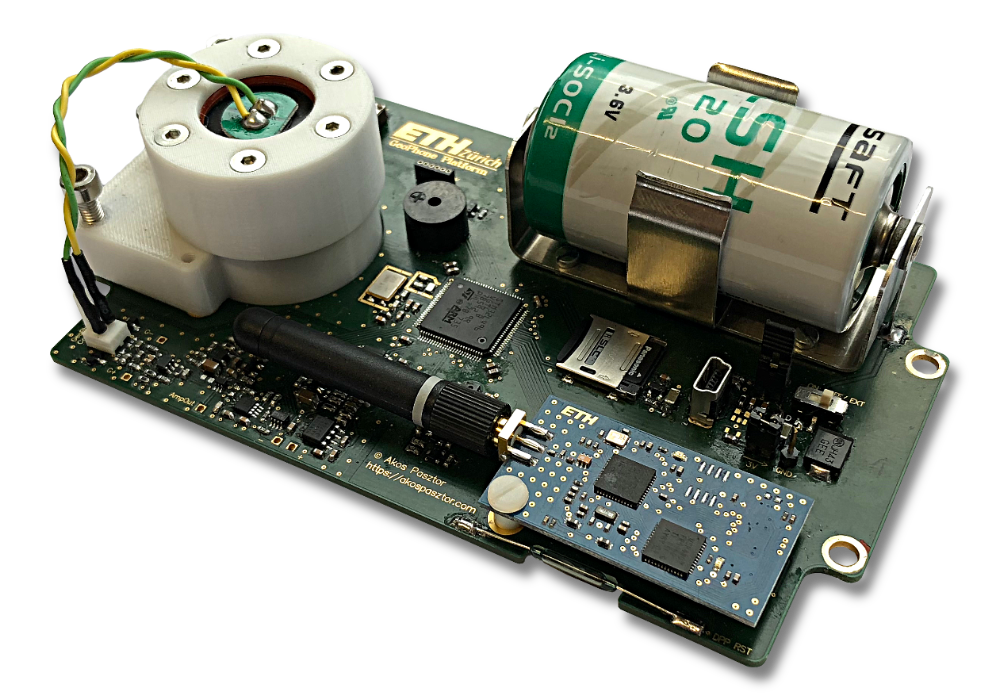
\includegraphics[width=\linewidth]{DPPs/GPP}
	\caption{Battery-powered geophone sensor node based on the \DPPtwo design.
	The lower ``application development board'' includes a geophone sensor, an analog low-power threshold-based wake-up circuit, and an ARM-Cortex M4~\cite{armCortexM4} as application processor.
	On top sits the same ``communication board'' as in \cref{fig:dpp2-cc430}.
	This design is currently deployed on the Hörnligrat of the Matterhorn~\cite{meyer2019IPSN}.}
	\label{fig:GPP}
\end{figure}

\end{subappendices}

% !TEX root = ../00_thesis.tex

\chapter[\triscale: Supporting Reproducibility in Networking]{\triscale: A Framework Supporting Reproducible Networking Experiments}
\label{ch:triscale}

\renewcommand{\ChapPath}{20_TriScale}
\renewcommand{\PathTab}{\ChapPath/Tables}

% \TODO{
% \begin{itemize}
%   \item upload new notebook on GitHub
% %   \item consider extending scalability
% %   \item unify scientist vs researchers
% \end{itemize}
% }

% !TEX root =  ../00_thesis.tex

% ------------------------------------------------------------------------------
% Global Positioning
The design of a system is not truly completed until the system's performance has been evaluated. This evaluation must be performed in a way that can be reproduced by others to build confidence in the performance claims.
In this dissertation, we study the design of wireless \CPS and we therefore are directly concerned by the challenge of performing reproducible performance evaluation of networking protocols.
Thus, in this chapter, we tackle the challenge of reproducibility in experimental networking research in general, beyond the sole context of low-power wireless networking (the main focus of this dissertation).
% The \triscale framework presented here is applicable to networking in general~(\cref{fig:chapter_triscale}); as such, the scope of this chapter extends


% ------------------------------------------------------------------------------
% Context
Achieving reproducibility in networking experiments requires a concrete methodology, which is currently missing.
The design and data analysis of experiments raise questions such as: How many runs to perform? How to account for the variability of networking experiments?
Despite the best intentions, researchers often answer these questions differently, which impairs the reproducibility of the entire evaluation.
Moreover, it is currently unclear how to formalize reproducibility, let alone assess whether performance evaluation results are ``reproducible'' or not.

% ------------------------------------------------------------------------------
% What is the problem?

\begin{figure}
  \centering
  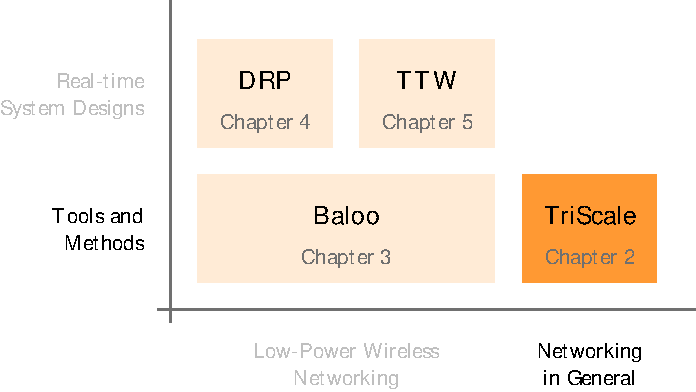
\includegraphics[scale=0.9]{chapter_triscale}
  \caption{This chapter presents \triscale, a framework supporting reproducible evaluations in networking research in general, beyond the sole context of low-power wireless.}
  \label{fig:chapter_triscale}
\end{figure}

% ------------------------------------------------------------------------------
% Claim
\fakepar{Claim}
We contribute to make experimental networking research more rigorous and more reproducible.
For the first time, we go beyond simple guidelines and propose a concrete methodology for designing networking experiments and analyzing their data.
We leverage this methodology to propose the first formalized definition of reproducibility for networking experiments.
Finally, we implement our methodology in a framework called \triscale, a first-of-its-kind tool that assists researchers by streamlining the design process and automating the data analysis.

\pagebreak
% ------------------------------------------------------------------------------
% Corresponding reference(s)
\begin{publi}

  The material from this chapter builds upon the work from Antonios Koskinas~\cite{koskinas2019reproducibility}. It relates to the following publications.

  \inlineRef%
  {Towards a Methodology for Experimental Evaluation in Low-Power Wireless Networking}%
  {Romain Jacob, Carlo Alberto Boano, Usman Raza, Marco Zimmerling, Lothar Thiele}%
  {CPS-IoTBench 2019. Montréal, Canada (April 2019)}

  \inlineRef%
  {TriScale: A Framework Supporting Reproducible Performance Evaluations in Networking}%
  {Romain Jacob, Marco Zimmerling, Carlo Alberto Boano,\\
  Laurent Vanbever, Lothar Thiele}%
  {\emph{Under submission.} (2020)}

\end{publi}

% !TEX root = ../00_thesis.tex

%-------------------------------------------------------------------------------
\section{Problem Setting}
\label{sec:triscale_intro}
%-------------------------------------------------------------------------------
% The problem is the variability of the evaluation process
The ability of reproducing experimental results is broadly considered a prerequisite for establishing a scientific claim.
In networking research, reproducibility%
\footnote{
A variety of terminologies is used to define the different aspects of reproducible research~\cite{plesser18terminology, barba2018Terminologies}.
In this dissertation, we refer to \emph{reproducibility} as the ability of different scientists to follow the steps described in published work using the \emph{same tools} and obtain the \emph{same results} within the margins of experimental error. This corresponds to ACM's definition of \emph{replicability}~\cite{acmBadges}.}
is a well-known issue due to the inherent variability of the experimental \mbox{conditions}.
\mbox{On the one hand}, the uncontrollable dynamics of real-world networks~\cite{matos18reproducible, burchfield09rfjungle} and the unsteady performance of hardware and software components~\cite{maricq2018Taming, blackburn2016Truth} can cause a large variability in the experimental conditions, which makes it hard to quantitatively compare different solutions~\cite{bajpai18dagstuhl_report}.
\linebreak
On the other hand, differences in the methodology used to design the experiment, analyze the data, and reason about the results impair the ability to reproduce and critically assess the validity of claims  made by other scientists.
Without reproducibility, any performance comparison is debatable, at best.

\begin{research_questions}
  \begin{description}

    \item[Question 1]
    Can we improve the reproducibility of performance claims of networking experiments?

    \item[Question 2]
  	Can we compare protocol performance in a statistically sound manner? In particular, how can we account for the inherent variability of the experimental conditions?
  \end{description}
\end{research_questions}

% Problem
\fakepar{The problem}
The community has relentlessly developed testbeds~\cite{nussbaum17testbeds} and data collection frameworks~\cite{yan18pantheon} to minimize the variability in experimental conditions.
In comparison, only a few works targeted \mbox{the design of a methodology} for networking evaluations~\cite{kritsis2018Tutorial}.
In this regard, the literature is limited to best practices and generic guidelines~\cite{bajpai19dagstuhl_guide, saucez2018Thoughts, sevenwaystofail}.

Experimental networking research suffers from the lack of a \emph{systematic methodology} specifying
% \begin{itemize}
	% \item
  (i)~how to concretely design an experiment, and
	% \item
  (ii)~how to analyze and report its results.
% \end{itemize}
Scientists are left with many open questions \emph{before} carrying out an experiment (\eg How many runs? How long should they be? When should they run?) and \emph{after} the data has been collected (\eg How to analyze and summarize the data in a concise yet accurate way?).

These open questions lead scientists to design similar experiments in different ways, which hinders comparability even when using the same tools~\cite{boano2018IoTBench}.
Furthermore, the lack of a common methodology for data analysis hampers the ability to recreate results even when all raw data are available (as known as \textit{computational reproducibility}~\cite{liu19computational}), a standard we argue that any scientific contribution should meet.
Finally, it is unclear how to concretely define reproducibility and assess whether a networking experiment is indeed ``reproducible''. When reproducibility is considered a prerequisite to any scientific claim, this question cannot be left unanswered.

% --------------------------------------
% Challenges
% --------------------------------------
\fakepar{The challenge}
We identify a set of requirements that an experimental methodology should meet in order to address this reproducibility problem.

\begin{features}

	\item[Generality]
	The methodology is applicable to a wide range of metrics, evaluation scenarios (both emulated and real-world settings), as well as network types (both wired and wireless).

	\item[Conciseness]
	The methodology describes the experiment design and data analysis in a concise yet unambiguous way.
	This enables computational reproducibility while \mbox{minimizing} the use of highly-treasured space in research papers.

	\item[Robustness]
	The methodology accounts for the intrinsic variability of networking experiments.
	The uncertainty is quantified and the analysis does not presume the nature of the raw data distribution (\eg no assumption of normality).
	The uncertainty quantifies the variation in performance that we expect to observe shall the experiments be repeated; in other words, the statistics used are not only descriptive but also predictive.

	\item[Rationality]
	The methodology rationalizes the experiment design and helps answering questions such as: How many runs? How long should they be? When should they run?
	This allows to minimize the number of experiments while collecting enough data to meet the desired level of confidence.

\end{features}

\fakepar{Our solution}
This chapter presents \triscale, a framework that meets all the above requirements for supporting researchers in the design and analysis of networking experiments.
We make the following contributions:

\begin{itemize}
	\item
	We propose a methodology for designing networking experiments and analyze their data.
	This methodology is grounded on non-parametric statistics~(\cref{sec:stats}), which provides performance reports that are both robust and clear.
	Our methodology rationalizes the experimental design process and quantifies the reproducibility of an experiment.

	\item
	We implement this methodology in \triscale, a framework that assists its user in designing experiments and automating data analysis~(\cref{sec:triscale}).

	\item
	As a case study, we use \triscale to compare congestion-control schemes using the Pantheon data collection framework~\cite{yan18pantheon} and show how \triscale improves on the legibility and confidence in the results~(\cref{sec:triscale_eval}).
	Additional examples using low-power wireless protocols running on the FlockLab testbed~\cite{lim2013FlockLab} illustrate the generality of the framework.
	Finally, we showcase the scalability of \triscale: the data analysis completes within seconds for millions of data points~(\cref{sec:triscale_implementation}).

	\item
	Finally, we make \triscale openly available~(\cref{append:triscale_artifacts}) for the networking community to use, extend, and build upon.
\end{itemize}
\triscale does not ``solve'' the entire reproducibility problem; in particular, it does not handle the data collection (see discussion in \cref{sec:going_further}).
\triscale does however fill a critical gap towards reproducible networking evaluations by providing a consistent methodology for the design of networking experiments and the analysis of their data.

% !TEX root = ../00_thesis.tex

%-------------------------------------------------------------------------------
\section{Overview of \triscale}
\label{sec:triscale_overview}
%-------------------------------------------------------------------------------

This section provides a high-level description of \triscale.
First, we illustrate how \triscale clarifies the interpretation of the results of networking experiments with a concrete example~(\cref{subsec:triscale_intro_example}),
then we present the core principles of \triscale and introduce the structure of the framework~(\cref{subsec:triscale_overview}).

\afterpage{
\begin{landscape}
  \begin{figure}
    \centering
    \begin{subfigure}[t]{0.48\linewidth}
        \centering
       	\href{\triscalefig{Figure-1a}}{
        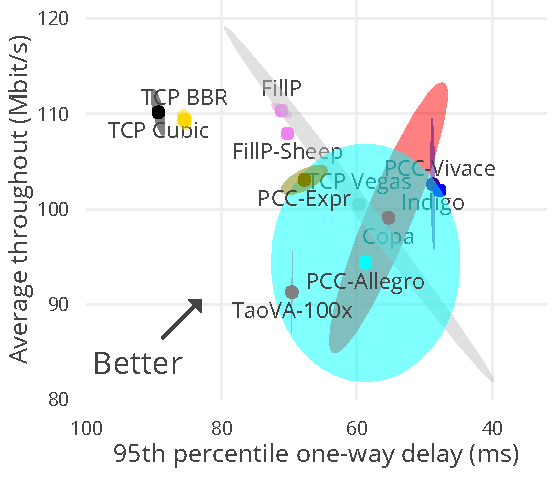
\includegraphics[scale=1]{Figures/plot_zoom_pantheon}}

        \caption{Data analysis and visualization reproduced from~\cite{yan18pantheon}. The dots represent the mean performance of the runs; the ellipses represent the $(1-\sigma)$ variation across runs.}
        \label{fig:example_pantheon}
    \end{subfigure}%
    \hfill
    \begin{subfigure}[t]{0.48\linewidth}
        \centering
        \href{\triscalefig{Figure-1b}}{
        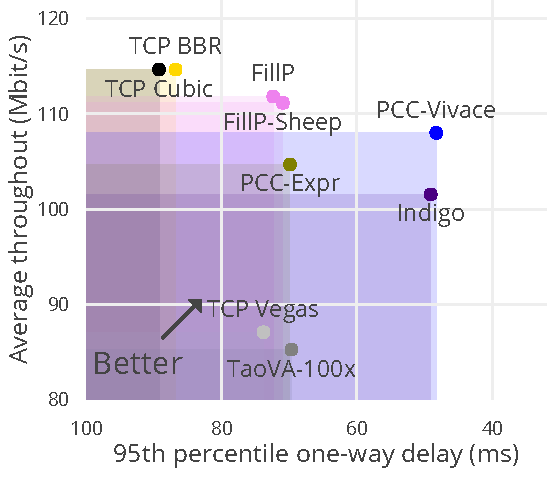
\includegraphics[scale=1]{Figures/plot_zoom_triscale}}

        \caption{Data analysis and visualization produced by \triscale. The dots represent the KPIs of each scheme. Shaded areas represent dominance regions: \emph{scheme~$A$} performs better than \emph{scheme~$B$} if the KPI of~$B$ lies in the dominance region of~$A$.}
        \label{fig:example_triscale}
    \end{subfigure}
    \caption{%
    The same data may be analyzed in different ways. \Cref{fig:example_triscale} illustrates the output of a data analysis performed by \triscale. Compared with \Cref{fig:example_pantheon}, the interpretation of the results is more intuitive: The performance of each scheme is reduced to a single point (\triscale's KPIs), which makes the comparison between the schemes unambiguous.
    \triscale's KPIs are not arbitrary: they are robust statistics estimating, with a given confidence level, the expected performance if the experiment was repeated (see~\cref{subsec:KPIs}). As such, the KPIs inherently account for the variability in the results.
    \capt{Experiment settings: 1 flow, 10 runs, 30\s runtime, emulated network (sample data from the congestion-control case study~\cref{sec:triscale_eval}).}}
    \label{fig:example_pantheon_triscale}
  \end{figure}
\end{landscape}
}


%-------------------------------------------------------------------------------
\subsection{Shortcomings in the Data Analysis}
\label{subsec:triscale_intro_example}

Let us assume you are a networking researcher discovering the field of congestion control and trying to understand the strengths and weaknesses of the state-of-the-art.
Luckily, the community has developed useful tools such as Pantheon~\cite{yan18pantheon}, a data collection framework that facilitates comparisons between different schemes.

You are especially interested in comparing the average throughput and one-way delay of long-running full-throttle flows, \ie stable flows whose only throttling/limiting factor is the congestion control.
You start with one flow and evaluate performance using the MahiMahi~\cite{netravali2015mahimahi} emulator (integrated in Pantheon), following the same settings as in the original paper~\cite{yan18pantheon}, \ie~10~runs of 30~seconds each. You collect data for the 17 schemes available at the time of your experiment.

Pantheon focuses on collecting data, not on their interpretation. Yet, the interpretation is not trivial. Consider for example the data shown in \Cref{fig:example_pantheon} (reproduced from~\cite{yan18pantheon}). Multiple questions arise:

\begin{itemize}

    % Hard to compare
    \item
    Can the schemes be compared?
    It appears that \textit{Vegas} performs better than \eg \textit{TaoVA-100x}.
    However, the ellipses capture the variability of results across multiple runs: more precisely, they represent the $(1-\sigma)$ variation across runs.
    What can you then conclude about the actual performance of these schemes?
    Can you conclude anything when ellipses are overlapping?
    For example, can you say that \textit{Vegas} performs better than \textit{PCC-Expr}?

    % Confidence? Are results trustworthy?
    \item
    What is the confidence in the comparison? Intuitively, the results of \eg \textit{PCC-Allegro}, which has a large variability, are ``less trustworthy'' than \eg \textit{FillP-Sheep}, for which you cannot even see the ellipse on the graph. But can you quantify the confidence in the result?

    % Impact of the runtime on the results?
    \item
    Is a runtime of 30~seconds (the default setting) really long enough to capture the long-running performance of the various schemes?

    % Are the results reproducible?
\end{itemize}


These questions relate to the \feature{Robustness} and \feature{Rationality} requirements mentioned in~\cref{sec:triscale_intro}.
The data analysis shown in \Cref{fig:example_pantheon} leaves these questions unanswered.
Worse, the analysis may suggest wrong interpretations: the ellipses are a two-dimensional representation of the standard deviation across the runs, which suggests that one expects about 68\% of the data points to fall in that region.
However, this is correct \textbf{only if} the underlying distribution is normal, which is hardly ever true (\cref{sec:stats}).

Let us now compare the \emph{same raw data}, but analyzed using \triscale (\Cref{fig:example_triscale}).
The points in the plot represent \triscale's Key Performance Indicators (KPIs).
A KPI is defined as the estimate of a given percentile of one performance metric distribution.
For example: with 10 runs, we collect 10 samples of the performance metric ``average throughput''.
Based on these 10~samples, we can \emph{estimate} some properties of the underlying distribution of ``average throughput'' (\ie the \emph{unknown} distribution one would obtain with infinitely many samples).
\triscale's KPIs estimate percentiles of that underlying distribution with a certain confidence.
In \Cref{fig:example_triscale}, the ``average throughput'' KPI is defined as the estimate of the 25th percentile with a 75\% confidence level; in other words, the KPI has a 75\% probability to correctly estimate the 25th percentile of the distribution (more details in \cref{subsec:KPIs}).

Since KPIs are individual points, they unambiguously compare different schemes.
\triscale shows, for example, that \textit{Vegas} is not generally better than \textit{TaoVA-100x}: each performs better in either delay or throughput (\Cref{fig:example_triscale}).
Furthermore, \textit{PCC-Expr} performs strictly better than \textit{Vegas}, whereas \Cref{fig:example_pantheon} suggests the opposite.
The KPIs in \Cref{fig:example_triscale} can be interpreted as follows:\emph{
with a 75\% probability, 75\% of the runs will yield a performance at least as good as the KPI value} (\ie higher throughput and lower delay).

Observe that \textit{Copa} and \textit{PCC-Allegro} are no longer present in \Cref{fig:example_triscale}.
Indeed, \triscale first verifies whether the schemes have ``converged''; that is, it checks whether the performance metrics have reached stable values (\cref{subsec:test_convergence}).
These two schemes eventually converge, but it often takes more than 30 seconds.
In \Cref{fig:example_triscale},
\emph{the KPIs are representative of the ``long-running'' performance} (\ie the performance expected if the scheme would run ``forever'') with a 95\% probability.

\fakepar{Conclusion}
Tools like Pantheon~\cite{yan18pantheon} support data collection, but leave to the researcher to design the experiments and analyze the data, leading to ambiguous interpretations and non-reproducible results.
\triscale aims to fill this gap.
\afterpage{
\begin{landscape}
  \begin{figure}
  	\centering
  	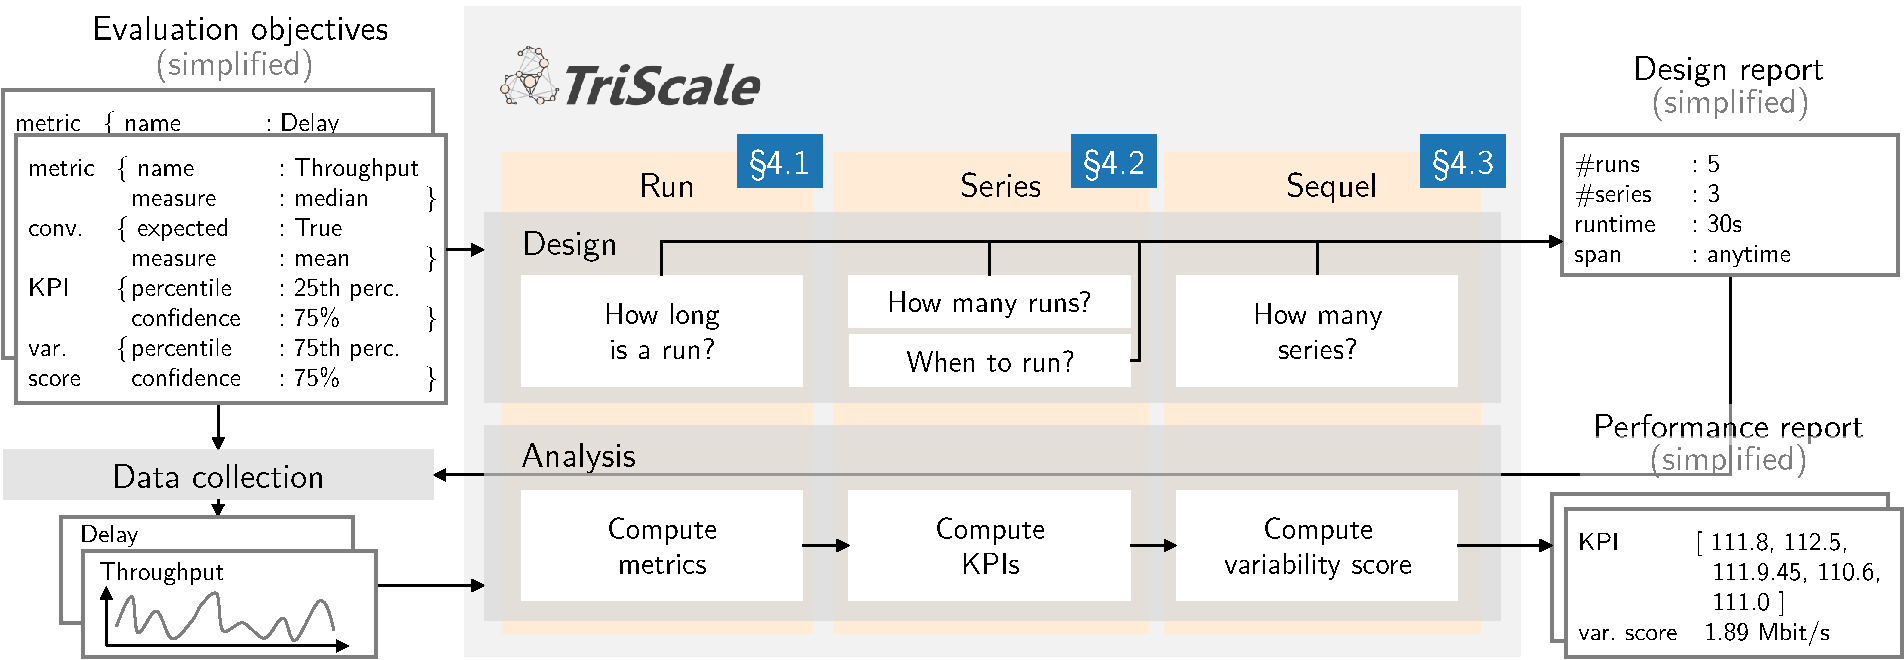
\includegraphics[width=0.955\linewidth]{triscale_overview_flat}
  	\caption{Overview of \triscale.
  		\capt{\triscale is a framework supporting the design and data analysis of networking experiments.
  		\triscale assists the user in the design phase with a systematic methodology to answer important experiment design questions such as ``How many runs?'' and  ``How long should the runs be?''. After the data has been collected, \triscale supports the user by automating the data analysis. The framework implements robust statistics that handle the intrinsic variability of experimental networking data and return expressive performance reports as well as a variability score.
  		}
  		}
  	\label{fig:overview}
  \end{figure}
\end{landscape}
}


%-------------------------------------------------------------------------------
\subsection{Methodological Core Principles}
\label{subsec:triscale_overview}

We now introduce how \triscale supports the design and analysis of networking experiments. The structure and inputs/outputs of the \triscale framework are illustrated in \Cref{fig:overview}.

\fakepar{Experiment design}
\triscale achieves \feature{Rationality}~(\cref{sec:triscale_intro}) by formalizing the evaluation definition and by streamlining the design of experiments.
The design phase starts with the definition of the evaluation objectives: for each performance dimension, the user defines the metric, the convergence requirements, a KPI, and a variability score.
From these inputs, \triscale returns the minimal number of runs (\emph{\#runs}) and \mbox{series} (\emph{\#series}) necessary to compute the chosen KPIs and variability scores; that is, \emph{how many runs to perform}.
Using the data from a few test runs, \triscale can assess whether the length of a run (the \emph{runtime}) is suitable; \ie \emph{how long a run should be}.
Finally, \triscale uses network profiling information to avoid time-dependent bias in the experiments; \ie it tells \emph{when the experiment should be carried out} (the \emph{span}).

In the congestion-control example presented previously, the evaluation objectives are the following.
The metrics' measures for throughput and delay are the median and 95th percentile, respectively.
The KPIs are chosen as the 25th and 75th percentiles with 75\% confidence, for which \triscale returns a minimum of 5 runs.
Convergence is expected and initial tests reveal that \textit{PCC-Allegro} and \textit{Copa} almost never converge within 30\s~(see \cref{sec:triscale_eval}).
As experiments are carried out in emulation, there is no time dependency and therefore it does not matter when the experiment is performed~(\ie \emph{span: anytime}).


\fakepar{Data analysis}
\triscale achieves \feature{Robustness} (\cref{sec:triscale_intro}) by
applying carefully-chosen statistical methods, verifying that their hypotheses hold for the collected data, and automating the computations.
In particular, once the experiment has been designed and the data collected, the raw data is passed to \triscale for analysis.
The analysis is divided into three timescales: \emph{runs}, \emph{series}, and \emph{sequels} (hence the name of \triscale):\\
%
% \begin{description}
%
%   \item[Runs]
  A \textbf{run} is one execution of the evaluation scenario (\eg a 30\s execution of one congestion-control scheme).
  The raw data from one run are analyzed to compute the performance metrics defined in the evaluation objectives.
  This timescale leads to one number per run and per metric~(\cref{subsec:metrics}).\\
  %
  % \item[Series]
  A \textbf{series} is a set of runs performed closely in time (\eg in the same day).
  Multiple runs allow to account for the inherent variability in the experiments.
  This timescale leads to one number per series and per metric, \ie \triscale's KPIs~(\cref{subsec:KPIs}).\\
  %
  % \item[Sequels]
  A \textbf{sequel} is a repetition of a series, performed at a later point in time (\eg a week, a month, or a year later).
  \triscale uses sequels (\ie a set of series) to compute a variability score which captures the long-term variability of the KPIs.
  This timescale leads to one number per metric (\cref{subsec:repeatability}).
%
% \end{description}

In the previous example, \triscale returns a pair of KPIs per scheme, which allow to unambiguous compare the different schemes with a quantified confidence (in this case, 75\% -- see \cref{fig:example_triscale}).

% !TEX root = ../00_thesis.tex

%-------------------------------------------------------------------------------
\section{Backgrounds on Statistics}
\label{sec:stats}
%-------------------------------------------------------------------------------

This section briefly discusses some background on statistics which is relevant to performance evaluation.

\fakepar{Descriptive and predictive statistics}
A statistic is a number computed from a data set using a mathematical formula.
A statistic can always be calculated and provides a factual description of the underlying data.
This is referred to as a \emph{descriptive statistic}.
However, certain statistics have also some \emph{inference} power; that is, based on the collected data, one may infer the shape of the underlying data distribution, which is unknown. These are referred to as \emph{predictive statistics}.

Predictions are always uncertain and often rely on certain hypotheses. If the hypotheses hold for the collected data, then the statistic estimates some property of the underlying distribution (\eg mean, median, \etc) with a quantifiable level of confidence. One can then predict the expected values of data samples that have not been collected.
One common hypothesis for predictive statistics is that the collected data is \emph{independent and identically distributed} (\iid); informally, this means that the underlying distribution of the data does not change and that successive data samples are not correlated.
It is also common to presume the \emph{nature of the data distribution} (\eg a normal or a Poisson distribution), which allows to make ``better'' predictions with less data.
It is paramount to keep in mind the hypotheses underlying a statistical prediction.

\begin{example}
  One can compute the mean $\mu$ and standard deviation $\sigma$ of a data sample.
  {If} the underlying data distribution is normal (the hypothesis), {then} we can infer that about 68\% of all data points (the distribution) will be contained in $\mu \pm \sigma$.
  However, \textbf{if the distribution is not normal, $\mu$ and $\sigma$ are only descriptive statistics};
  \ie they do not predict anything about the underlying data distribution.
\end{example}

\fakepar{Statistical methods}
Many common statistical methods assume Gaussian distributions (\ie normally distributed data).
However, literature reports that experimental data is rarely normal~\cite{maricq2018Taming,schmid2014measuring} and hence recommends using \emph{non-parametric statistics}; \ie statistics that do not make any assumption on the nature of probability distributions.
Furthermore, it is important to consider \emph{robust statistics}, \ie statistics that are not overly skewed by outliers (common in networking data).
There are two main classes of statistical approaches: hypothesis testing and estimation.
%
% \begin{itemize}
    %
    % \item
    \emph{Hypothesis testing} consists in formulating a so-called null hypothesis, that the test aims to reject. Based on the collected data, one computes the probability, called the \mbox{$p$-value}, that the null hypothesis is correct.
    If the \mbox{$p$-value} is sufficiently low, the null hypothesis is rejected and considered proven incorrect.
    %
    % \item
    \emph{Estimation} consists in computing confidence intervals (CIs) for a given parameter (\eg the median of a distribution).
    A CI is always associated a confidence level (\eg a 95\%~CI) which is the probability that the interval includes the true value of the parameter.
    For example, $[a,b]$ is a 95\%~CI for the median if the true median value is between $a$ and $b$ with 95\% probability (or better).
%
% \end{itemize}

CIs are more legible than $p$-values: ``\textit{CIs provide a mechanism for making statistical inferences that give information in units with practical meaning}''~\cite{cumming2001CI}.
Furthermore, the level of confidence of an estimation only depends on the sample size. In other words, estimations can be used to guide the experimental design. By setting the desired level of confidence, one defines the (minimal) number of samples required.
This is a key property that \triscale leverages.

\fakepar{Reproducibility is a predictive statistic}
Informally, reproducibility is the principle that the ``same experiment'' leads to the ``same results''. Thus, assessing reproducibility entails predicting that future data (\ie the results of a newly-performed experiment) will be the same as the known data (\ie the results of previously conducted experiments): this is a prediction.
Thus, assessing reproducibility requires making certain hypotheses on the data.
It is hence crucial to \emph{(i)~}choose statistics with hypotheses compatible with actual networking data, and to \emph{(ii)~}verify that the hypotheses do hold for the data that one collects.
To this end, \triscale makes use of non-parametric statistics and verifies that their hypotheses hold for the collected samples.

% !TEX root = ../00_thesis.tex
%-------------------------------------------------------------------------------
\section{Designing \triscale}
\label{sec:triscale}
%-------------------------------------------------------------------------------

In this section, we first describe the data analysis performed by \triscale and how the analysis procedure is linked to the design of experiments~(\cref{subsec:metrics} to \cref{subsec:repeatability}).
We then illustrate how the formalism introduced by \triscale allows to unambiguously describe an entire performance evaluation with only a handful of parameters~(\cref{subsec:parameters}).
Thereafter, we detail the robust and non-parametric statistical methods used by \triscale~(\cref{subsec:triscale_stats}), and discuss how the framework assists a user in deciding the required time span for a series of runs~(\cref{subsec:network_profiling}).
We finally show how \triscale helps assessing the reproducibility of experiments by computing a variability score~(\cref{subsec:reproducibility}).

%-------------------------------------------------------------------------------
\subsection{Runs and Metrics}
\label{subsec:metrics}

\afterpage{
\begin{figure}
    \centering
    \begin{subfigure}{\linewidth}
        \centering
       	\href{\triscalefig{Figure-3a}}{
        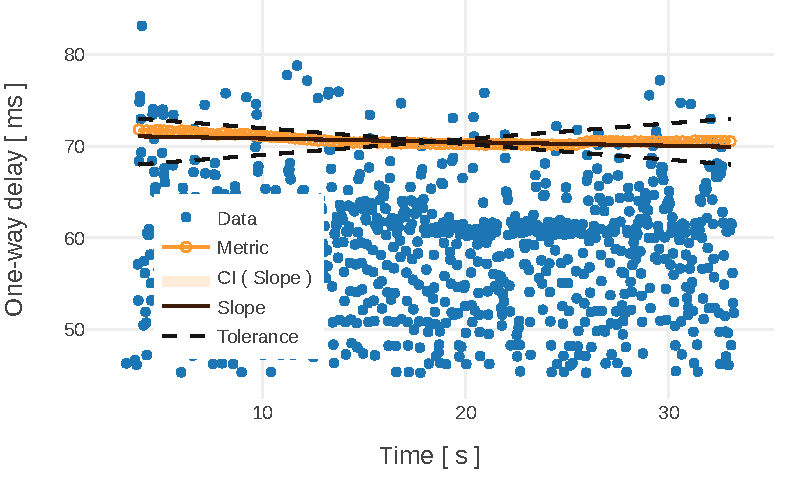
\includegraphics[scale=1]{Figures/plot_example_metric.pdf}}
        \caption{\raggedright Raw data (one-way delay) and metric data (95th percentile).}
        \label{fig:analysis_metric}
    \end{subfigure}



    \begin{subfigure}{0.45\linewidth}
        \centering
       	\href{\triscalefig{Figure-3b}}{
        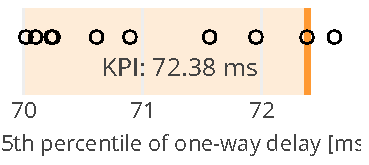
\includegraphics[scale=1]{Figures/plot_example_KPI.pdf}}
        \caption{Runs' metric data and corresponding KPI value.}
        \label{fig:analysis_kpi}
    \end{subfigure}
    %
    \hfill
    \begin{subfigure}{0.45\linewidth}
        \centering
     	  \href{\triscalefig{Figure-3c}}{
        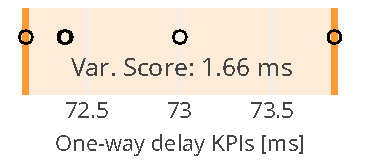
\includegraphics[scale=1]{Figures/plot_example_var_score.pdf}}
        \caption{Series' KPI data and corresponding variability score.}
        \label{fig:analysis_score}
    \end{subfigure}
    \caption{Example plots produced by \triscale during the data analysis.
    \Cref{fig:analysis_metric}: computation of the metric (95th percentile on one-way delay) with convergence test (confidence 95\%, tolerance 1\%).
    \Cref{fig:analysis_kpi}: computation of the KPI (75th percentile with 75\% confidence).
    \Cref{fig:analysis_score}: computation of the variability score (25-75th percentiles with 75\% confidence).
    \capt{Sample data from the case study (\cref{sec:triscale_eval}) for the \textit{FillP} congestion-control scheme.}}
    \label{fig:analysis_examples}
\end{figure}
}

A \triscale's metric evaluates a performance dimension across one run. For example, a metric may be the average throughput achieved by a congestion-control scheme over 30\s runtime of a full-throttle flow.
Computing a metric takes the following inputs.

\fakepar{Inputs}
\custommini),  &\\
          & tolerance & $t$   &(\textit{default: 1\%})    &\}
    \end{tabular}
  \item The raw data of the run.
  \end{itemize}
}%


In its current implementation, \triscale supports only percentiles as measures.
This can be easily extended to offer a catalog of common measures for networking experiments~(mean, max, fairness index, \etc).

\fakepar{Procedure}
If the run is expected to convergence, \triscale starts by performing a convergence test.
The purpose of the convergence test is to assess whether the metric measure has reached a ``stable'' value by the end of the run, and therefore if it is a good estimate of the ``long-running'' performance.

To test this, \triscale divides the raw data in 200 chunks. First, it considers the first 100 chunks (\ie the first half of the data) and computes a first value of the measure. Then, \triscale adds one chunk of data and recomputes a new measure value (\ie using the first 101 chunks). The process repeats until all chunks are used, leading to a set of 100 measure values. \triscale performs its convergence test~(detailed in \cref{subsec:triscale_stats}) on the measure data.
This procedure (i)~tests what we are interested in (\ie the convergence of the \emph{measure}, not of the protocol in general) and (ii)~smooths the effects of ramp-up time by computing the first measure with already half of the run data.
If the test is passed, \triscale returns the median of the measure data as the metric measure for the run.

\begin{remark}
  The choice of 200 chunks is arbitrary. We choose this value as it is practical and leads to 100 measure data samples. Empirically, we found this is enough to reliably test for the metric convergence.
\end{remark}

\begin{remark}
  If there are less than 200 raw data points, \triscale reduces the number of chunks to the number of data points.
  \triscale (arbitrarily) sets a minimum of 20 data points for a convergence test.
\end{remark}

\fakepar{Outputs}
\custommini{%
\begin{itemize}
  \item
  The result of the convergence test (if performed),
  \item
  The metric value for the run,
  \item
  Textual logs; plot of the input data and metric (\Cref{fig:analysis_metric}).

\end{itemize}
}

\fakepar{Link to the experiment design}
The computation of \triscale metrics is linked to the definition of the \emph{runtime}; \ie how long a run should be.
If the evaluation scenario is terminating (\eg transmit 1\MB through a link), the runtime must be long enough to complete the task.
If the evaluation is ``long-running'' (\eg one-way delay in a full-throttle flow), the runtime must be long enough for the metric (the one-way delay) to converge (convergence test details in \cref{subsec:triscale_stats}).
\triscale can analyze preliminary experiments to estimate the required runtime: by performing increasing long runs and test for convergence~(illustrated in \cref{sec:triscale_eval}).

%-------------------------------------------------------------------------------
\subsection{Series and KPIs}
\label{subsec:KPIs}
%-------------------------------------------------------------------------------

\triscale's key performance indicators (KPIs) evaluate performance dimensions across a series of runs.
Performing multiple runs allows to mitigate the inherent variability of the experimental conditions.
KPIs capture this variability by estimating percentiles of the (unknown) metric distributions.
Concretely, a \triscale KPI is a one-sided CI of one percentile; \eg a lower-bound for the 75th percentile of the delay metric estimated with a 75\% confidence level.
Computing a KPI takes the following inputs.

\fakepar{Inputs}
\custommini{%
  \begin{itemize}
    \item
    The {KPI} definition\\
    \begin{tabular}{@{\quad}l@{\quad}r@{\;\;:\;\;}l@{\quad}l}
      \{  & percentile & $p$ &\\
          & confidence & $C$&\}
    \end{tabular}
    \item
    The metric data (computed from a series of runs).
\end{itemize}}


\fakepar{Procedure}
To compute the KPI (\ie to compute a CI for a given percentile), \triscale uses the Thompson's method (\cref{subsec:triscale_stats}), which requires the input data to be \iid.
Thus, \triscale starts by performing an independence test~(\cref{subsec:triscale_stats})
on the metric data before computing the KPI.

\fakepar{Outputs}
\custommini{
\begin{itemize}
  \item The result of the independence test,
  \item The KPI value for the series of runs,
  \item Textual logs; plot of the metric data and corresponding KPI (\Cref{fig:analysis_kpi}).
\end{itemize}
}

\fakepar{Link to the experiment design}
The computation of \triscale KPIs is linked to the definition of the number of runs in a series (\emph{\#\,runs}) and the series time span (\emph{span}).
The minimal number of runs in a series directly follows from the definition of the KPI; \ie the percentile to estimate $p$ and the desired confidence level $C$.
The series time span refers to the time interval used for scheduling the runs in a series (\ie when to run the experiment).
This is important because networks often feature time-dependent conditions; for example, there may be systematically more cross-traffic during daytime than nighttime. Failing to account for such dependencies may bias the results and yield wrong conclusions.
\triscale helps the experimenter handling this problem with a dedicated analysis module called ``network profiling'' (described in~\cref{subsec:network_profiling}).



%-------------------------------------------------------------------------------
\subsection{Sequels and Variability Score}
\label{subsec:repeatability}
%-------------------------------------------------------------------------------


\triscale's variability score evaluates the variations of KPI values across repetitions of the experiment (\ie a series of run), which we call sequels.
Performing sequels allows to detect long-term variations in the KPI values which ultimately quantify the reproducibility of the experiment.
Concretely, a variability score is a two-sided CI for a symmetric pair of percentiles, \eg the 75\% CI for the 25-75th percentiles of the delay KPI.
Computing a variability score takes the following inputs.

\fakepar{Inputs}
\custommini{%
\begin{itemize}
  \item
  The {variability score} definition\\
  \begin{tabular}{@{\quad}l@{\quad}r@{\;\;:\;\;}l@{\quad}l}
    \{  & percentile & $p$ (or 1-$p$) &\\
        & confidence & $C$&\}
  \end{tabular}
  \item
  The KPI values of each sequel.
\end{itemize}}

\fakepar{Procedure}
The procedure is the same as for the KPI: The Thompson's method requires the input data to be \iid~(\cref{subsec:triscale_stats}), thus \triscale performs an independence test on the KPI data before computing the variability score.

\fakepar{Outputs}
\custommini{%
\begin{itemize}
  \item
  The result of the independence test,
  \item
  The variability score value for the entire sequels,
  \item
  Textual logs; plot of the KPI data and corresponding variability score (\Cref{fig:analysis_score}).
\end{itemize}}

\fakepar{Link to the experiment design}
The computation of the variability score is linked to the definition of the number of series (\emph{\#series}).
The minimal number of series directly follows from the definition of the variability score; \ie the percentile to estimate $p$ and the desired confidence level $C$.

%-------------------------------------------------------------------------------
\subsection{Formalism Brings Conciseness}
\label{subsec:parameters}
%-------------------------------------------------------------------------------

\afterpage{
\begin{landscape}
  \begin{table}
      \centering
      \caption{Exemplary evaluation parameters of typical networking use cases.
      \capt{$^{*}$\triscale returns the minimal number of runs (\#runs) and series (\#series) based on the definition of KPI and variability score, respectively.}}
      \input{\PathTab/triscale_parameters.csv}
      \label{table:triscale_param}
  \end{table}
\end{landscape}
}

\triscale formalizes the definition of the evaluation objectives. For each performance dimension, the experimenter defines a metric and convergence requirements~(\cref{subsec:metrics}), a KPI~(\cref{subsec:KPIs}), and a variability score~(\cref{subsec:repeatability}).
\triscale links these objectives with the experiment design, resulting in four additional parameters: the number of runs per series (\emph{\#\,runs}), the number of series (\emph{\#\,series}), the length of a run (\emph{runtime}), and the time span of a series (\emph{span}).

Thanks to this formalism, \triscale meets the \feature{Conciseness} requirement:
Altogether, these 12 parameters are sufficient to \emph{formally describe the entire performance evaluation} such that it can (eventually) be reproduced.
In particular, since the data analysis in \triscale is automated and deterministic, documenting these parameters guarantees computational reproducibility (the ability to recreate the results when all raw data are available~\cite{liu19computational}).

\Cref{table:triscale_param} shows a few examples of concrete parameter settings for typical networking evaluation objectives.
For example, evaluating the latency of a real-time protocol requires high confidence levels for extreme percentiles.
This very quickly increases the number of runs that one must perform:\\
\inlineitem
  at least 90 runs for estimating the 95th percentile with 99\% confidence;\\
\inlineitem
  at least 299 runs for estimating the 99th percentile with 95\% confidence.\\
This illustrates that it is ``easier'' to increase the confidence level of an estimate than to estimate a more extreme percentile with the same confidence level.
Note that both \emph{\#runs} and \emph{\#series} are only derived based on the definition of the KPI and variability score; these parameters are not influenced by the runtime or the time span of an experiment.

The second use case in \Cref{table:triscale_param} (bottom rows) illustrates two different perspectives on ``averages'', using delay as an example:\\
\inlineitem
  If the metric is the median and the KPI the 90th percentile, one can conclude that 90\% of the runs have a median delay equal or better than the KPI value.\\
\inlineitem
  If the metric is the 90th percentile and the KPI the median, one can conclude that, in half of the runs, the 90th percentile of the delay in the run be equal or better than the KPI.\\
Both are ``averages'' but with different meanings and different requirements in terms of number of runs.


%-------------------------------------------------------------------------------
\subsection{Statistics in \triscale}
\label{subsec:triscale_stats}
%-------------------------------------------------------------------------------

\triscale uses carefully chosen statistical methods.
As discussed in~\cref{sec:stats}, networking performance evaluations should focus on statistics that are both \emph{robust} (\ie that can tolerate outliers) and \emph{non-parametric} (\ie that do not make any assumption on the nature of the data distribution).
This section describes the three statistical methods used in \triscale. We first present the convergence test used in the computation of metrics (\cref{subsec:metrics});
This test is based on the \mbox{Theil-Sen} linear regression~\cite{theil1992RankInvariant, sen1968Estimates}.
We then introduce the computation of confidence intervals using Thompson's method~\cite{thompson1936Confidence}, which requires the data to be \iid. Thus, to verify this assumption, \triscale integrates an independence test that we present last.

%-------------------------------------------------------------------------------
\fakepar{Convergence test}
\label{subsec:test_convergence}
When an evaluation aims to estimate the ``long-running'' performance (\ie the expected performance if the run would run “forever”), one must verify whether the runs are long enough to produce reliable estimates.

To verify this, \triscale implements a convergence test based on the Theil-Sen linear regression~\cite{theil1992RankInvariant, sen1968Estimates}.
The approach computes the slope of the regression line as the median of all slopes between paired values.
A $C$\% confidence interval (CI) for the slope is defined as the interval containing the middle $C$\% of slopes between single pairs.
\triscale convergence test is passed if the $C$\% CI for the regression is included in the tolerance value ($\pm$\,$t$\%).
To test the convergence of a run, \triscale uses the confidence $C$ and tolerance $t$ parameters specified in the evaluation objectives (\Cref{sec:triscale_overview}); $C$ and $t$ are set to 95\% and 1\% by default.

Such a test is sensitive to the scale of the input data.
To remove this dependency, \triscale first maps the data to $[-1, 1]$ using a linear transformation then performs the convergence test on the scaled data.
Hence, the convergence test becomes dimensionless and the same tolerance value can be used for different evaluations without introducing bias.
An example of the Theil-Sen slope (brown, solid), its CI (light orange, solid), and tolerance (black, dotted) is shown in \Cref{fig:analysis_metric}.

%-------------------------------------------------------------------------------
\fakepar{Confidence Intervals}
\triscale defines KPIs~(\cref{subsec:KPIs}) and variability scores~(\cref{subsec:repeatability}) based on CIs for distribution percentiles, which can be computed using Thompson's method~\cite{thompson1936Confidence}, a robust and non-parametric approach.

Let us denote by $P_p$, the $p$-th percentile of a distribution and $\mathbb{P}(X)$ the probability of an event $X$.
By definition, every data sample $x$ is smaller than $P_p$ with probability $p$ (and larger with probability $1-p$).
For a sorted list of \iid samples $x_i$ (where $i = 1 .. N$), the probability that $P_p$ lies between two consecutive samples follows the binomial distribution~\cite{thompson1936Confidence}:
\begin{equation}
    \mathbb{P}(x_k \leq P_p \leq x_{k+1}) = \binom{N}{k} p^k(1-p)^{N-k}, \quad k = 0 .. N
\end{equation}
where we assume $x_0 \rightarrow - \infty$ and $x_{N+1} \rightarrow +\infty$. From this result, it follows that the probability of $P_p$ to be larger than any sample $x_m$ (where $1\leq m < N/2$) can be computed as:
\begin{align}
  \nonumber
    \mathbb{P}(x_m \leq P_p)
      &= \mathbb{P}(x_{N-m+1} \geq P_{1-p})\\
  \label{eq:lb}
      &= 1 - \sum_{k=0}^{m-1} \binom{N}{k} p^k(1-p)^{N-k}
\end{align}
\Cref{eq:lb} provides the upper- and lower-bound required for computing of CIs.
See~\cite{schmid2014measuring} for more details.

This approach provides robust estimates for distribution percentiles and \emph{does not make any assumption on the nature of the underlying distribution}.
It does, however, require that the data samples are \iid. \triscale checks whether this hypothesis holds using an independence test, described below.

%-------------------------------------------------------------------------------
\fakepar{Independence test}
Estimating the percentile of a distribution requires often (if not always) that the samples are \iid (\cref{sec:stats}); this is also the case for Thompson's method~\cite{thompson1936Confidence}.
\triscale implements an empirical independence test to verify whether the \iid assumption holds.
This independence test is applied to the metric data (resp. KPI data) before the computation of a KPI (resp. a variability score).
This poses the particular challenge that the number of data samples may be very small (\eg 3 or 5 KPI values). \triscale's independence test must therefore not be too strict.

The test is divided in two steps. First, \triscale tests whether the data appear \emph{weakly stationary} (\ie no trend and constant autocorrelation structure~\cite{brockwell1991Time}). \triscale verifies this empirically using its convergence test with a confidence of 50\% and tolerance of 10\%; these ``loose'' parameters are used to compensate for (very) small sample sizes.
Second, \triscale computes the \emph{sample autocorrelation coefficients}, denoted by $\widehat{\rho_k}$, which measure the linear dependency between values of a weakly stationary data series.
A series of size $N$ is \iid with 95\% probability if $|\widehat{\rho_k}| \leq 1.95/\sqrt{N}$ for $k \geq 1$~\cite{brockwell1991Time}.

\fakeparQM{What if the tests fail}
The experimenter is responsible for designing the evaluation in such a way that the collected data will (likely) pass the tests.
\triscale facilitates this by guiding the choice of runtime to pass the convergence test and informing about any network time dependencies~(\cref{subsec:network_profiling}) to pass the independence test.
Yet, the data may still be correlated or unstable, leading to failing tests (see examples in ~\cref{sec:triscale_eval}).
Even in such cases, the data still contain useful information.
\triscale metrics, KPIs, or variability scores can be computed, however since the corresponding hypotheses do not hold, the statistics are \emph{only descriptive}~(\cref{sec:stats}); they do not predict the expected performance, and in particular they cannot (and should not be used to) assess the reproducibility of the experiment.

%-------------------------------------------------------------------------------
\subsection{Network Profiling}
\label{subsec:network_profiling}

\begin{figure}
    \centering
   	\href{\triscalefig{Figure-4}}{
    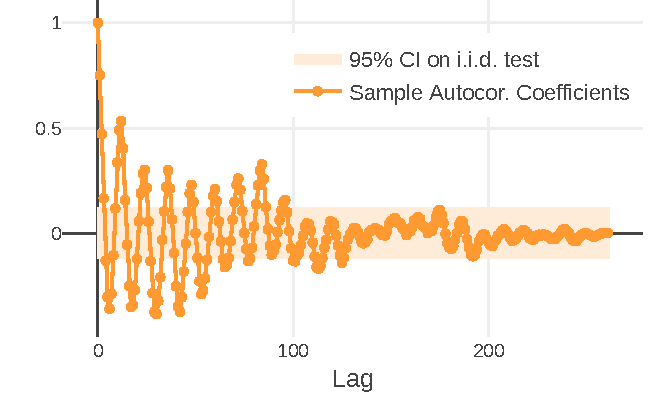
\includegraphics[scale=1]{Figures/plot_flocklab_autocorr.pdf}}

    \caption{Autocorrelation plot for the wireless link quality on FlockLab, based on the raw data collected by the testbed maintainers~\cite{jacob2019datasetLQE} (data from August 2019).
    \capt{The dataset contains one test every two hours. The first peak at lag 12 (\ie 24h) reveals the daily seasonal component. The data also show another at lag 84; which corresponds to one week. Indeed, there is less interference in the weekends than on weekdays: this creates a weekly seasonal component.}}
    \label{fig:flocklab_autocorr}
\end{figure}

\triscale assists the user in deciding on the time span for a series of runs, \ie when should the run be performed in a series. This is important to avoid biasing the evaluation results with time dependencies in the experimental conditions.
Indeed, it is common for real-world networks to exhibit periodic patterns.
For example, there may be a lot more cross-traffic (\ie interference) at specific times. In the statistics literature, these patterns are called \emph{seasonal components}.
Neglecting these may result in biased experiments leading to wrong conclusions, as illustrated in the case study below.

\fakepar{Case study: low-power wireless}
We run a simple evaluation of Glossy~\cite{ferrari2011Glossy}, a low-power wireless protocol based on synchronous transmissions~(\cref{sec:ST}). Glossy includes as parameter the number of retransmissions of a packet, called $N$. We investigate the impact of two values of $N$ on the reliability of Glossy, measured as the packet reception ratio (PRR). We define our KPI as the median with 95\% confidence level.
Refer to \cref{append:triscale_artifacts} for the complete case study.

We collect data using the FlockLab testbed~\cite{lim2013FlockLab}.
This testbed is located in an office building, where we expect more interference during daytime than nighttime.
Thus, we schedule a series of 24 runs randomly within one day.\\
  \inlineitem $N=1$ leads to a PRR of 88\%,\\
  \inlineitem $N=2$ leads to a PRR of 84\%.\\
In other words, it appears that doing two retransmissions (instead of one) reduces reliability.

The experiment leads to this (incorrect) conclusion because we have neglected a second seasonal component of the FlockLab testbed: there is a weekly time dependence, revealed by \Cref{fig:flocklab_autocorr}.
To account for this dependency, one must schedule runs with a span of at least one week. When comparing again the performance of Glossy but with tests spanning over a week\\
  \inlineitem $N=1$ leads to a PRR of 80\%,\\
  \inlineitem $N=2$ leads to a PRR of 88\%,\\
which better matches our knowledge about the performance of Glossy.

\fakepar{Conclusion}
This simple example illustrates that using a high confidence level is not enough to avoid drawing wrong conclusions due to the variability in the experimental conditions.
On a real network, short-term variations are unpredictable and (often) unavoidable. This is why it is important to perform multiple runs in a series: it increases the chances to do the experiment in the whole range of favorable to unfavorable conditions.

However, we illustrated that systematic patterns are also present. In other words, there are times where there is consistently more or less interference. Knowing about these dependencies is important to
  ensure fairness in the comparison between protocols, and
  enable reproducibility of the evaluations.
The series span must be long enough such that it does not matter when the series actually starts (\eg a weekend or a weekday)

\triscale integrates a network profiling function that analyzes link quality data (such as those available at~\cite{jacob2019datasetLQE}) and searches for seasonal components in the link quality data. This helps the experimenter detecting (sometimes unexpected) time dependencies, thus choosing a suitable time span for series of runs.


%-------------------------------------------------------------------------------
\subsection{Assessing Reproducibility}
\label{subsec:reproducibility}

Reproducibility refers to the ability of obtaining ``the same'' results when performing ``the same'' experiment.
In statistics, such property can be investigated using \textit{equivalence testing}~\cite{lakens2017Equivalence}, which checks whether the values of some parameter of interest (\eg the median) obtained for different samples are sufficiently close to be considered ``the same''.
Unfortunately, there is no general way to define ``sufficiently close''; one must define in advance a threshold for the equivalence test based on expertise.
Then, how to assess reproducibility of networking experiments? How to design a ``reproducibility test'' that fairly adapts to different networking contexts and different metrics?
After some failed attempts, we conclude that defining a generic threshold for equivalence testing in networking might not be possible. But it may not be necessary.

We argue that the most important is to confidently estimate the variability of the results, which \triscale computes with its variability score~(\cref{subsec:repeatability}).
This score \emph{quantifies reproducibility}: the larger the score, the less reproducible the results are.
Shall a binary cut between ``reproducible'' and ``not reproducible'' be desired, a threshold can be set based on the variability score; \eg ``Results are said reproducible when the variability score is less than 20\mbps.''.
Such a threshold can only be context-specific; thus, deciding on threshold values relates more to benchmarking and therefore goes beyond the scope of \triscale~(see discussion in \cref{sec:going_further}).

% !TEX root = ../00_thesis.tex

%-------------------------------------------------------------------------------
\section{\triscale in Action}
\label{sec:triscale_eval}
%-------------------------------------------------------------------------------

\begin{figure}
    \centering
    \begin{subfigure}{\linewidth}
        \centering
       	\href{\triscalefig{Figure-4}}{
        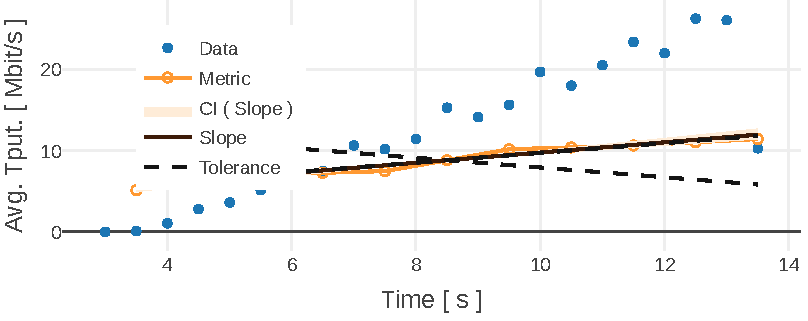
\includegraphics[scale=1]{Figures/plot_ledbat_10_runtime.pdf}}
        \caption{10\s runtime}
        \label{fig:10s}
    \end{subfigure}

    \begin{subfigure}[b]{\linewidth}
        \centering
       	\href{\triscalefig{Figure-4}}{
        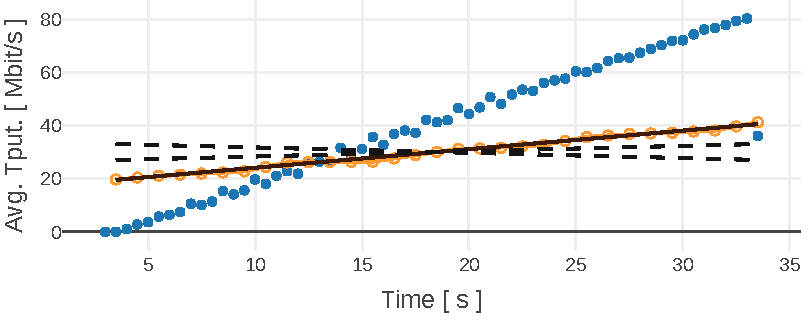
\includegraphics[scale=1]{Figures/plot_ledbat_30_runtime.pdf}}
        \caption{30\s runtime}
        \label{fig:30s}
    \end{subfigure}

    \begin{subfigure}[b]{\linewidth}
        \centering
       	\href{\triscalefig{Figure-4}}{
        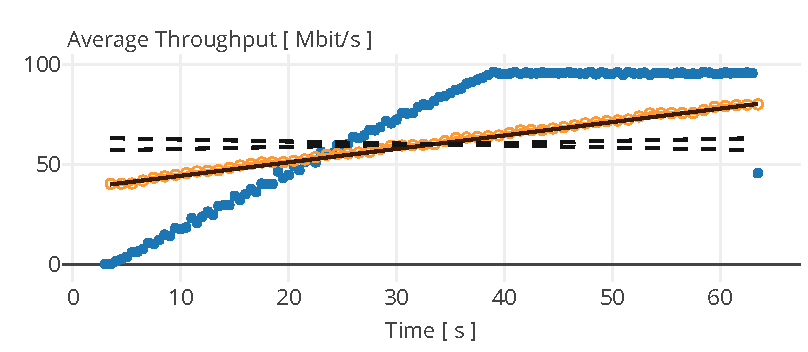
\includegraphics[scale=1]{Figures/plot_ledbat_60_runtime.pdf}}
        \caption{60\s runtime}
        \label{fig:60s}
    \end{subfigure}
    \caption{Egress throughput of \textit{LEDBAT} in MahiMahi, calibrated to the real path from AWS California to Mexico~\cite{yan18pantheon}.
    \capt{\mbox{A runtime} of 30\s is clearly not sufficient for \textit{LEDBAT}'s throughput to converge (\Cref{fig:30s}). The scheme does converge eventually (\Cref{fig:60s}), but even with 60\s runtime, \triscale's convergence test fails: the impact of the start-up phase is too important. Two possible solutions are to (i)~increase the runtime or (ii)~prune the start-up time from the raw data.}}
    \label{fig:ledbat_convergence}
\end{figure}

This section continues the case study introduced in \cref{subsec:triscale_intro_example}.
We compare the performance of 17 congestion-control schemes using Pantheon~\cite{yan18pantheon}. We evaluate the throughput and one-way delay of long-running full-throttle flows, \ie stable flows whose only throttling/limiting factor is the congestion control.
For a fair comparison between the schemes, we use the MahiMahi emulator~\cite{netravali2015mahimahi} (integrated in Pantheon). We focus on a single flow scenario and use the calibrated path from AWS California to Mexico.%
\footnote{\href{https://pantheon.stanford.edu/result/6539/}{pantheon.stanford.edu/result/6539/}}
The complete case study is available as complementary materials~(\cref{append:triscale_artifacts});
we present here only a fraction of it and focus on showcasing how \triscale avoids certain shortcomings in the experiment design and analysis. Finally, we illustrate how to quantify performance variability: a prerequisite for assessing reproducibility (\cref{subsec:reproducibility}).

%-------------------------------------------------------------------------------
\fakepar{Convergence time}
The first step in the design of an evaluation is to decide how long the runs should be.
Since all schemes are different, it is hard to know a priori the minimum runtime for which the various schemes actually converge.

We test runtimes from 10 to 60\s and check whether the 17 congestion-control schemes pass \triscale's convergence test (\cref{subsec:triscale_stats}).
With a runtime of 30\s, only twelve schemes often pass the test; others (\textit{Verus}, \textit{PCC-Allegro}, \textit{Copa}, and \textit{QUIC Cubic}) converge in less than half the runs.
Furthermore, \textit{LEDBAT} never pass the test, even with a runtime of 60\s.
The reason for this is shown in~\Cref{fig:ledbat_convergence}: the inner working of the protocol causes the throughput to ramp-up in the first 38\s of runtime and then converge to about 92\mbps.
If one uses 30\s runtime without checking for convergence, the computed average throughput is about 40\mbps, which is a wrong estimation of \textit{LEDBAT} ``long-running'' throughput.
By performing the convergence test, \triscale hints the experimenter about the need to either increase the runtime, or prune the start-up time in the raw data.

\begin{figure}
    \centering
   	\href{\triscalefig{Figure-5}}{
    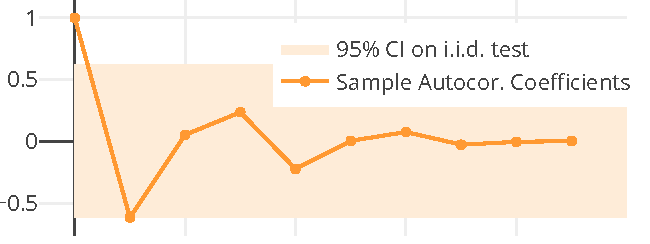
\includegraphics[scale=1]{Figures/plot_webrtc_autocorr_passed.pdf}}\\
   	\href{\triscalefig{Figure-5}}{
    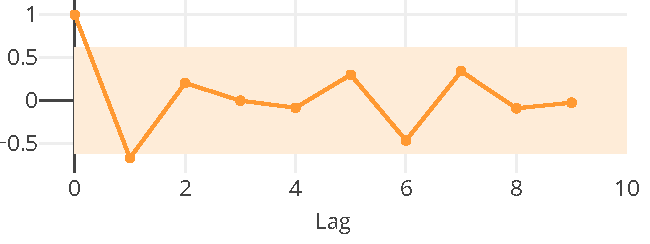
\includegraphics[scale=1]{Figures/plot_webrtc_autocorr_failed.pdf}}
    \caption{Autocorrelation coefficients for two exemplary series of \textit{WebRTC}.
    \capt{The upper series passes the autocorrelation test, whereas the lower series does not: this is an artifact induced by the small number of samples (here: 10 samples).}
    }
    \label{fig:webrtc_autocorr}
    \vspace{-1cm}
\end{figure}

%-------------------------------------------------------------------------------
\fakepar{Independence tests}
The computation of \triscale's KPIs and variability scores requires the samples to be \iid (\cref{subsec:triscale_stats}).
However, the number of runs and series performed in an evaluation tends to be small (as experiments are both time- and resource-consuming), which limits the significance of the independence test.
\Cref{fig:webrtc_autocorr} illustrates this problem: it shows the autocorrelation plot for two series for \textit{WebRTC}.
The autocorrelation coefficients must be in the shaded gray area for the test to pass.
In this case, the upper series passes the test, whereas the lower one does not.
However, there is no clear difference in the correlation structure of the two series: the lower series does not seem significantly more correlated than the upper one.
All other series of \textit{WebRTC} pass the independence test, which hints that the failed series is merely an artifact induced by the small number of runs in the series (in this example, 10 runs per series).
In such cases, it is important that the experimenter critically assesses \triscale's results and increase (when necessary) the number of runs or series to improve the significance of results -- or overrule the test~(discussion in \cref{sec:going_further}).

%-------------------------------------------------------------------------------
\fakepar{Evaluation in emulation}
Using the MahiMahi emulator for the evaluation is expected to be the most favorable setting to test the reproducibility of the congestion-control schemes, since it allows to recreate the exact same test conditions and therefore improves the comparability between the runs.
This however has an unexpected side-effect: while they appear to have a very stable behavior, \emph{TCP BBR} and \emph{TCP Cubic} would always fail the independence test. Actually, these two schemes are designed to use all the available bandwidth and, since MahiMahi artificially sets the latter to a fixed value, the two schemes always reach the exact same throughput.
This leads to the exact same metric values; in other words, the throughput is \emph{perfectly correlated} across runs.
Naturally, this is an artifact of the experiment: the independence test will always fail if all data samples have the same value.

\triscale always computes the KPIs and variability scores, even if the independence test fails. The experimenter is responsible to judge whether there is indeed true correlation in the data, or if one can overrule the test result and proceed with the analysis.
In the example of \emph{TCP BBR} and \emph{TCP Cubic}, one can proceed.

%-------------------------------------------------------------------------------
\fakepar{KPIs}
We illustrated in~\cref{subsec:triscale_intro_example} how \triscale's KPIs allow to unambiguously compare the performance of different schemes.
\Cref{fig:example_triscale} shows the KPI for the average throughput (resp. one-way delay), defined as the estimate of the 25th (resp. 75th) percentile with a 75\% confidence level for 10 runs with 30\s runtime.
We use 30\s to compare with the Pantheon results shown in~\Cref{fig:example_pantheon}).
However, five schemes fail to converge sufficiently often and thus do not appear in~\cref{fig:example_triscale}.

%-------------------------------------------------------------------------------
\fakepar{Variability scores}
Although \triscale's KPIs unambiguously compare the performance of diverse schemes, they only consider one series of runs, which does not indicate how reproducible the results actually are.
\triscale investigates reproducibility using sequels and quantifies the expected variability in the KPI values with a variability score~(\cref{subsec:repeatability}).
In this case study, we define the variability score as the difference between the 75th and 25th percentiles, estimated with 75\% confidence.
We compute the variability scores for our two performance dimensions (average throughput and one-way delay -- \Cref{fig:score_matrix}).
The scores can be interpreted as follows: with 75\% probability, the variability scores (orange bars) give the magnitude of variation expected (shall one perform infinitely many series) in the middle 50\% of KPI values.
Hence the variability score quantifies reproducibility: the larger the score, the less reproducible the results are.

\begin{remark}
  \triscale's variability scores are absolute values with units (\eg in \mbps). Arguably, it may be useful to use relative scores (in percentages) to compare the scores of different protocols.
\end{remark}

%-------------------------------------------------------------------------------
\fakepar{Conclusion}
This case study only considers emulation and one emulated path. As such, it does not aim to fully evaluate the performance of the different congestion-control schemes.
Rather, it illustrates how \triscale may be used for an actual performance evaluation and the importance of carefully choosing the parameters of an experiment; such as the runtime~(\Cref{fig:ledbat_convergence}).
We highlight two important takeaways:
\begin{itemize}
  \item It is important to critically consider \triscale's results: the tests are intentionally conservatives to limit the risk of false positives (\eg not detecting correlation in the data),
  \item It is useful to collect more samples than strictly necessary: it improves the significance of the tests and therefore limits the risk of false negatives.
\end{itemize}

\begin{figure}
    \centering
   	\href{\triscalefig{Figure-6}}{
    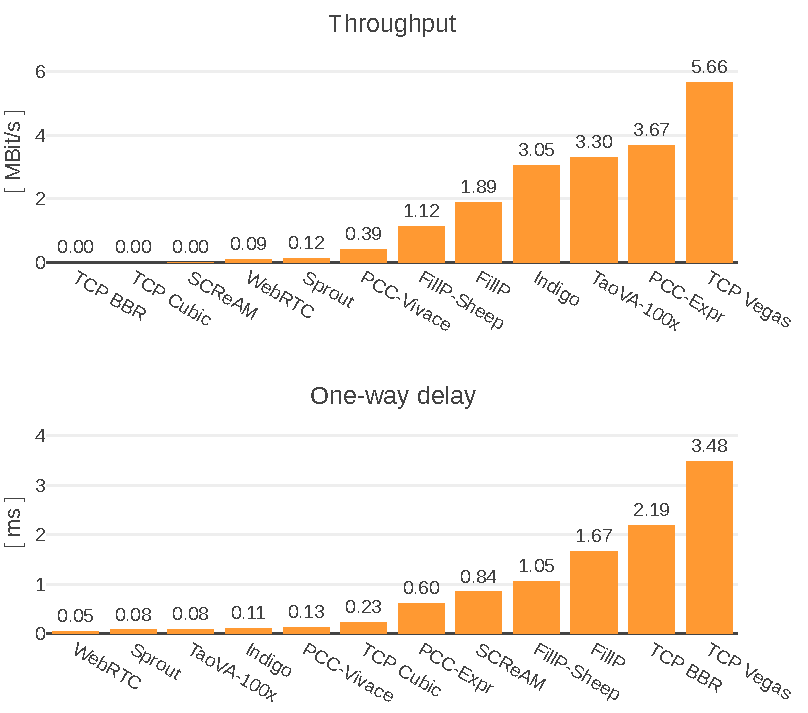
\includegraphics[width=\linewidth]{Figures/plot_score_matrix.pdf}}
    \caption{Variability scores computed by \triscale for the performance dimensions throughput and delay.
    \capt{
      In this example, the variability scores are computed as the 25th to 75th percentile interval estimated with 75\% confidence.
      From the variability scores, the user gets a quantification, with a 75\% probability, of the range of variation in the KPI values for 50\% of the series.
      The variability scores hence quantify reproducibility: the larger the scores, the less reproducible the results are.}
    }
    \label{fig:score_matrix}
\end{figure}

% !TEX root = ../00_thesis.tex

%-------------------------------------------------------------------------------
\section{Implementation and Scalability of \triscale}
\label{sec:triscale_implementation}
%-------------------------------------------------------------------------------

%-------------------------------------------------------------------------------
\subsection{Python Package}

We implement \triscale in Python ($\approx$1000 lines of code) and make it open source~(\cref{append:triscale_artifacts}).
\triscale's API contains one function for each timescale of the data analysis; \ie the computation of metrics, KPIs, and variability scores.
Docstrings contain detailed information about the functions usage.
Our implementation relies on standard scientific packages such as NumPy~\cite{numpy}, Pandas~\cite{pandas}, SciPy~\cite{scipy}.
As the use of non-parametric statistics is not (yet) widespread, we had to implement some of the statistics used by \triscale (in particular the computation of CI using Thompson's method).
We hope to see these functions integrated in a future release of SciPy.

It is important to produce useful visualizations to support the experimenter.
Thus, we paid a particular attention to the plotting functions in \triscale.
\triscale uses Plotly~\cite{plotly} to create interactive plots: one can zoom in and out in the plots, toggle the visibility of individual traces, read data point values on hover, \etc
All the plots in this chapter are produced using \triscale and are ``clickable'': figures are hyperlinks leading to dynamic versions of the plots.


%-------------------------------------------------------------------------------
\subsection{Scalability of \triscale Data Analysis}
\label{subsec:scalability}

We evaluate the scalability of \triscale with respect to computation time; \ie how does the data analysis time scales with increasing input sizes.
We only consider the time required for performing computations; other outputs such as logs and plots (\eg \Cref{fig:analysis_metric}) are excluded.
The complete scalability evaluation (including data, plots, and discussions) is available as complementary materials~(\cref{append:triscale_artifacts}).
Generally, the computation time for the data analysis in \triscale scales linearly with the input size~(\Cref{table:scalability}): it is fast (less than 1\s for one million data points on a commodity laptop) and overall negligible compared to the data collection time.


\begin{table}
    \centering
    \caption{Scalability evaluation.
    \capt{\triscale data analysis is fast and scales well with increasing input sizes. The most time-consuming element is the convergence test~(\cref{subsec:test_convergence}) which is performed before the computation of metrics. Still, it generally takes less than one second for inputs (\ie the number of raw measurements in a run) of up to one million data points.}}
    \input{\PathTab/triscale_scalability.csv}
    \label{table:scalability}
\end{table}

% !TEX root = ../00_thesis.tex
%-------------------------------------------------------------------------------
\section{Discussion, Limitations, and Future Work}
\label{sec:going_further}
%-------------------------------------------------------------------------------

%-------------------------------------------------------------------------------
% Data collection
\fakepar{Data collection}
\triscale is not responsible for the execution of networking experiments, \ie it does not perform the data collection (\cref{sec:triscale_overview}).
Frameworks specialized in data collection, such as Pantheon~\cite{yan18pantheon}, already exist and \triscale can be integrated into these frameworks to create a fully-automated experimentation chain.
Other examples include low-power wireless testbeds~\cite{schuss2017Competition, schuss2018DCube, lim2013FlockLab} and networking facilities~\cite{banerjee2015PhantomNet, duplyakin19cloudlab, nussbaum17testbeds}, which could be combined with \triscale to build full-fledged benchmarking infrastructures~\cite{boano2018IoTBench}.


%-------------------------------------------------------------------------------
% Human-in-the-loop
\fakepar{Human-in-the-loop}
\triscale automates the data analysis and implements tests that verify whether the required hypotheses hold.
However, these tests are not perfect: the confidence will never be 100\%. Moreover, the significance of such tests is always low when the sample sizes are small; \eg the independence test may flag correlated data when ``correlation'' is only an unlucky random variation (\Cref{fig:webrtc_autocorr}).
\triscale raises flags to avoid missing clear issues (\eg \textit{LEDBAT} convergence time -- \Cref{fig:ledbat_convergence}), but the experimenter must always critically assess \triscale results and potentially overrule them; \eg neglecting the correlation of perfect throughput for \emph{TCP~BBR} and \emph{TCP~Cubic}.

%-------------------------------------------------------------------------------
% Ranking
\fakepar{Ranking solutions}
\triscale compares performance, but it does not rank. The results of a networking evaluation are always relative to a specific network and evaluation scenario.
It is not trivial to generalize and claim that a solution~A is better than a solution~B. This problem relates to benchmarking and multi-objective optimization, which goes beyond the scope of \triscale.

%-------------------------------------------------------------------------------
% Community guidelines
\fakepar{Community guidelines}
\triscale formalizes evaluation objectives (\cref{subsec:parameters}), but it does not dictate which parameters to use.
Similarly, \triscale quantifies the variability of an experiment~(\cref{subsec:repeatability}), but it does not conclude whether the experiment is reproducible~(\cref{subsec:reproducibility}).
\triscale provides a framework to describe evaluations and analyze the data in a consistent and statistically sound manner. It is now up to the networking communities to set their own standards, parameters to use, and acceptable requirements; similar to what is already done in other disciplines~\cite{gallen14minimumreq}).

% !TEX root = ../00_thesis.tex

%-------------------------------------------------------------------------------
\section{Related Work}
\label{sec:relWorks}
%-------------------------------------------------------------------------------

%-------------------------------------------------------------------------------
% The reproducibility crisis
The reproducibility of experiments and comparability of results are cornerstones of the scientific method.
In recent years, several studies have highlighted the inability of scientists from various disciplines to reproduce their own experimental results~\cite{baker16reproducibility, peng15crisis}, often due to sloppy research protocols and faulty statistical analysis~\cite{boisvert2016Incentivizing, blackburn2016Truth, schmid2014measuring}.
This problem has also been recognized within computer science~\cite{collberg15reproducibility, vitek11systems}, where experiments are seldom reproducible and artifacts rarely shared.


%-------------------------------------------------------------------------------
% Promoting reproducibility
\fakepar{Promoting reproducibility}
To address this ``\mbox{reproducibility} crisis''~\cite{baker16reproducibility}, several efforts aiming to incentivize a rigorous experimentation have gained momentum in computer science, including \eg ACM's badging system \mbox{for publications}~\cite{acmBadges}.
Especially in the networking community -- challenged by the need to carry out experiments on dynamic and uncontrollable conditions~\cite{burchfield09rfjungle, matos18reproducible} -- several workshops~\cite{bajpai18dagstuhl_report, cpsbench18cpsweek, reproducibility17sigcomm}, surveys~\cite{flittner2018artifacts_survey}, guidelines~\cite{bajpai19dagstuhl_guide, saucez2018Thoughts, kritsis2018Tutorial, sevenwaystofail}, as well as teaching activities~\cite{yan17learning} have raised awareness on the reproducibility problem and promoted better experimentation practices.
This large body of work mostly offers \emph{qualitative} statements on how an experiment should be performed and documented.
Such qualitative statements emphasize for example the need to carefully choose when and how often to sample data~\cite{bajpai19dagstuhl_guide}, or suggest which methodology to adopt during performance evaluations~\cite{kritsis2018Tutorial}.
However, there is no guarantee that following these recommendations leads to reproducible results, nor is there a concrete way to assess whether an experiment can be considered reproducible.

None of the existing works provide scientists with \emph{quantitative} answers about how to concretely perform an experiment, \eg how many runs should be completed and how long should they be.
\triscale fills this gap by providing quantitative answers to these questions with an experimental methodology grounded on robust non-parametric statistics.
\triscale also allows to assess and compare the reproducibility of experimental results by computing unambiguous performance indicators and variability scores.

%-------------------------------------------------------------------------------
% Tools supporting repeatability while experimenting
\fakepar{Supporting reproducibility}
A large number of experimental facilities and tools have been developed in recent years to aid scientists and practitioners in carrying out reproducible networking studies~\cite{nussbaum17testbeds}.
Testbeds such as EmuLab~\cite{white02emulab} and FlexLab~\cite{ricci07flexlab}, as well as emulation tools such as MiniNet~\cite{handigol12container} and MahiMahi~\cite{netravali2015mahimahi}, enable the creation of artificial network conditions using a given specification or passively-observed traffic.
Emulated conditions offer a more controlled environment than experiments faced with real-world traffic (\eg by transmitting data over the Internet~\cite{chun03planetlab, berman2014GENI}, cloud~\cite{duplyakin19cloudlab, bolze06grid5000}, or wireless interfaces~\cite{adjih15iotlab, ganu05orbit, massouri14cortexlab}).
Still, they suffer from performance variability caused by the underlying hardware and software components, which hampers reproducibility~\cite{maricq2018Taming}.
To overcome these problems, several solutions have been proposed~\cite{edwards15testbeds}: \eg revisiting  operating system libraries~\cite{tazaki13directcode}, using virtualization~\cite{handigol12container, kannan18bnv, koponen14nvp}, adaptable profiles~\cite{ricci2015Apt}, and fault patterns~\cite{angainor_website}.
Other tools have been developed to support mobility experiments~\cite{cho16phantomnet_repeatability, banerjee2015PhantomNet}, maximize the repeatability of interference generation~\cite{schuss19jamlabng}, and enable researchers to consistently evaluate congestion control schemes or transport protocols~\cite{yan18pantheon}.
Other works model the execution of experiments, and uses such models to quantify the similarity between different runs~\cite{sharma17framework,ferreira2017MetaAnalysis}.

While all aforementioned tools aim to improve reproducibility \emph{during} the experiments, \triscale assists researchers \emph{before} and \emph{after} their execution.
It does so by informing about the number and length of runs necessary to obtain a sufficient statistical significance, as well as by computing a score quantifying the variability of the results.
Hence, \triscale complements the existing body of literature promoting and enhancing reproducibility in networking research.

% !TEX root = ../00_thesis.tex

%-------------------------------------------------------------------------------
\section{Summary}

%What we presented
Establishing a consistent methodology for the design of networking experiments and the analysis of their data is a crucial step towards a more rigorous and reproducible scientific activity.
This chapter presented \triscale, the first concrete proposal in that direction.

% Key concept/novel idea
\triscale implements a methodology grounded on non-parametric statistics into a framework that assists scientists in designing experiments and automating the data analysis.
\triscale ultimately improves the legibility of results and helps quantifying the reproducibility of experiments, as highlighted in the case studies presented throughout the chapter.
% Takeaways
We expect \triscale's open availability to actively encourage its use by the networking community and promote better experimentation practices in the short term.
The quest towards highly-reproducible networking experiments remains open, but we believe that \triscale represents an important stepping stone towards an accepted standard for experimental evaluations in networking.



% Chapter appendices
\begin{subappendices}
\newpage
% !TEX root = ../00_thesis.tex
\section{Appendix -- Artifacts and Links}
\label{append:baloo_artifacts}

\subsection{Related Publications}

\inlineRef%
{Synchronous Transmissions Made Easy: Design Your Network Stack with Baloo}%
{Romain Jacob, Jonas Bächli, Reto Da Forno, Lothar Thiele}%
{EWSN 2019. Beijung, China (February 2019)}

\customLink{\faFileTextO}{Paper}{10.3929/ethz-b-000324254}{https://doi.org/10.3929/ethz-b-000324254}
\customLink{\faDesktop}{Presentation}{10.3929/ethz-b-000328814}{https://doi.org/10.3929/ethz-b-000328814}

\inlineRef%
{Creating a Flexible Middleware for Low-Power Flooding Protocols}%
{Jonas Bächli}%
{Master Thesis. ETH Zurich (June 2018)}

\customLink{\faBook}{Thesis}{10.3929/ethz-b-000270388}{https://doi.org/10.3929/ethz-b-000270388}

\subsection{Complementary Materials}
Complementary materials for this chapters are available on GitHub, together with the dissertation source files. For all links below, replace\\
\linkroot  by ``{github.com/romain-jacob/doctoral-thesis/blob/master}''

\customLink{\faFilesO}{\tex sources}{\linkroot/30\_Baloo/}{\linkrootURL/30\_Baloo/}
\customLink{\faFileImageO}{Figures}{\linkroot/30\_Baloo/Figures/}{\linkrootURL/30\_Baloo/Figures/}
% \customLink{\faCopyright}{\credit}{\linkroot/credits/30\_Baloo.pdf}{\linkrootURL/credits/30\_Baloo.pdf}
\customLink{\faGlobe}{Webpage}{romainjacob.net/baloo}{http://www.romainjacob.net/research/projects/baloo/}
%
\customLink{\faCode}{\baloo source code}{}{}
  \customLink{}{--- Documentation}{GitHub Wiki}{https://github.com/ETHZ-TEC/Baloo/wiki}
  \customLink{}{--- Latest release}{10.5281/zenodo.3510171}{https://doi.org/10.5281/zenodo.3510171}
  \customLink{}{--- ``This-version'' release}{10.5281/zenodo.3530632}{https://doi.org/10.5281/zenodo.3530632}
\customLink{\faChain}{Experiment data}{}{}
  \customLink{}{--- Latest release}{10.5281/zenodo.3510198}{https://doi.org/10.5281/zenodo.3510198}
  \customLink{}{--- ``This-version'' release}{10.5281/zenodo.3510214}{https://doi.org/10.5281/zenodo.3510214}

\end{subappendices}

% ~
% \newpage
% ~
% \pagestyle{empty}
% ~
% \newpage
% ~
% \newpage

% !TEX root = ../00_thesis.tex

\chapter[Synchronous Transmissions Made Easy with \baloo]{Synchronous Transmissions Made Easy:\\~Design Your Network Stack with \baloo}
\label{ch:baloo}

\renewcommand{\ChapPath}{30_Baloo}
\renewcommand{\PathTab}{\ChapPath/Tables}

% !TEX root =  ../00_thesis.tex

% ------------------------------------------------------------------------------
% Global Positioning
In the previous chapter, we discussed how to design and analyze networking experiments in general~(\cref{ch:triscale}).
In the rest of this dissertation, we will focus on low-power wireless networking, and more specifically on a technique called \emph{synchronous transmissions}.

% ------------------------------------------------------------------------------
% Context
Synchronous transmissions (\ST) refers to a wireless approach for broadcasting messages in a multi-hop network using flooding.
This is made efficient by letting multiple transmitters send the \emph{same packet} at the \emph{same time}; hence the name of \emph{synchronous} transmissions.%
\footnote{The name \textsl{concurrent transmissions} is also found in the literature.}
\ST has been proven highly reliable and energy efficient for low-power wireless networks.
Furthermore, \ST supports mobility by design thanks to the stateless logic of flooding-based communication.

% ------------------------------------------------------------------------------
% What is the problem?
Unfortunately, it is difficult to guarantee that multiple nodes actually send at the ``same time''.
The required precision on synchronization depends, \eg on the physical layer speed, the radio modulation speed or the encoding scheme.
For typical low-power wireless motes available today, the synchronization must be in the order of \us for \ST to work reliably.
Achieving such time synchronization requires to precisely control the timing of radio operations, which involves careful timer settings and interrupt handling.
The integration of such ``low-level software'' within a entire network stack is challenging.
Consequently, the adoption and development of \ST-based network stacks has been hindered by
the lack of usable and flexible design tools.

\begin{figure}
  \centering
  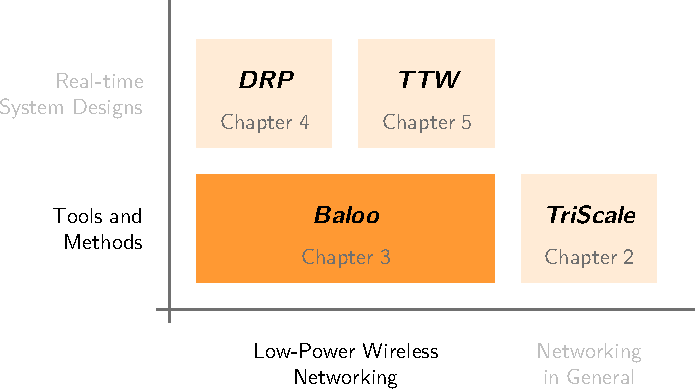
\includegraphics[scale=0.9]{chapter_baloo}
  \caption{Positioning of this chapter in the dissertation.
  \capt{This chapter presents \baloo, a design framework facilitating the implementation of low-power wireless networking protocols based on synchronous transmissions.}}
  \label{fig:chapter_baloo}
\end{figure}

% ------------------------------------------------------------------------------
% Claim
Thus, in this chapter, we study the feasibility of a design tool that would facilitate the development of network stacks based on \ST~(\cref{fig:chapter_baloo}); typically, such a tool would be useful for implementing our real-time protocol stacks (see \cref{ch:drp} and \cref{ch:ttw}).

\fakepar{Claim}
We propose and implement \baloo, a design framework for network stacks based on synchronous transmissions.
\baloo significantly lowers the entry barrier for harnessing the efficiency, reliability and mobility support of synchronous transmissions: users implement their protocol through a simple yet flexible API while \baloo handles all the complex low-level operations based on the users' inputs.

\baloo is flexible enough to implement a wide variety of network layer protocols, with only limited memory and energy overhead.

% ------------------------------------------------------------------------------
% Corresponding reference(s)
\begin{publi}

  The material from this chapter builds upon the work from Jonas Bächli~\cite{bachli2018Creating}. It relates to the following publication.

  \inlineRef{Synchronous Transmissions Made Easy: Design Your Network Stack with Baloo}{Romain Jacob, Jonas Bächli, Reto Da Forno, Lothar Thiele}{EWSN 2019. Beijung, China (February 2019)}

\end{publi}

% ------------------------------------------------------------------------------
% ------------------------------------------------------------------------------
% FORMER INTRO
% ------------------------------------------------------------------------------
% ------------------------------------------------------------------------------
% \newpage
% %Context
% \textsl{Synchronous Transmissions} (\ST) refers to a wireless communication technique that broadcast messages in a multi-hop network using flooding.
% This is made efficient by letting multiple transmitters send the \textsl{same packet} at the \textsl{same time}; henceforth the name of \emph{synchronous} transmissions.%
% \footnote{The name \textsl{concurrent transmissions} is also found in the literature.}
% \ST has been proven to be highly reliable and energy efficient, in particular for low-power wireless networks. Furthermore, flooding allows \ST to seamlessly support mobility by design.
% More informantion about \ST are presented in Introduction (\cref{ch:introduction}).
%
% %Problem
% Unfortunately, it is difficult to guarantee that multiple nodes actually send at the ``same time''.
% The required precision on synchronization depends \eg on the physical layer speed, the radio modulation speed or the encoding scheme.
% For typical low-power wireless motes available today, the synchronization must be in the order of \us for \ST to work reliably.
% Achieving such time synchronization requires to precisely control the timing of radio operations, which involves careful timer settings and interrupt handling.
% The integration of such ``low-level software'' within a entire network stack is challenging.
% Consequently, the adoption and development of \ST-based network stacks has been hindered by
% the lack of usable and flexible design tools.
%
% %Task and object
% Therefore, we developed \baloo: a flexible network stack design framework, designed to facilitate the development of protocols based on \ST. The key element of \baloo is a middleware layer which separates the radio management from the protocol implementation: \baloo provides a flexible application programming interface, while ensuring the correct timing of radio operations.
%
% %Findings
% \baloo is flexible enough to implement a wide variety of network layer protocols, with only limited memory and energy overhead.
% Most importantly \baloo makes \ST accessible: The software is open source and well documented.
% Since its development, \baloo has been used in a variety of projects, from both our team and external research groups.
% We believe that \baloo is an important enabler for a whole new class of Internet of Things applications leveraging the reliability, efficiency, and flexibility of \ST.

%
%
% This chapter presents \baloo, its design and the evaluation of its performance. We conclude with a brief description of projects that have been facilitated by \baloo, and finally discuss potential future developments, including standardization efforts.

% !TEX root =  ../00_thesis.tex

\section{Prolem Setting}
\label{sec:baloo_intro}

\squarepar{%
  Synchronous Transmissions (\ST) is an increasingly used wireless communication technology for low-power multi-hop networks. Popularized by Glossy~\cite{ferrari2011Glossy} in 2011, it has been proven to be highly reliable and energy efficient, as illustrated by the EWSN Dependability Competition ~\cite{schuss2017Competition}, where all wining solutions were based on \ST~\cite{escobar2018Competition,sommer2016Competition,lim2017Competition, escobar2019RedNodeBus, ma2019DeCoT} in the past four years (2016 to 2019).%
}

A \textsl{\ST primitive} refers to a protocol that efficiently realizes broadcast (\ie any-to-all communication) in bounded time, usually relying on \textsl{flooding}.
Flooding is a communication strategy that realizes broadcast by having all receivers of a packet retransmit this same packet to all their neighbours; the packet is thus ``flooded'' through the whole network. \ST makes flooding energy and time efficient by letting multiple wireless nodes transmit the packet \textsl{synchronously}, hence the name of \textsl{Synchronous Transmissions}. The successful reception of the packet can be achieved if the transmitters are tightly synchronized, thanks to \textsl{constructive interference} and the \textsl{capture effect}~\cite{yuan2013LetTalkTogether}.
The synchronization requirements vary from sub-\us to tens of \us, depending on the platform and modulation scheme~\cite{yuan2013LetTalkTogether}.
 %
%\footnote{Some background on flooding and \ST technology is provided in \cref{sec:baloo_overview}.}.
Such a broadcast primitive simplifies the design of network layer protocols: The underlying multi-hop network can be abstracted as a \textsl{virtual single-hop network} and thus be scheduled like a shared bus~\cite{ferrari2012LWB}.
One may refer to \cref{ch:introduction} for more details on \ST.

Since Glossy~\cite{ferrari2011Glossy}, many flavours of \ST primitives have been proposed to improve performance in terms of reliability, latency, and energy consumption.
To be more resilient to strong interference, Robust Flooding~\cite{lim2017Competition} is a primitive that modifies the RX-TX sequence from the original Glossy, whereas RedFixHop~\cite{escobar2016RedFixHop} uses hardware acknowledgements to minimize the number of retransmissions required.
Instead, some primitives aim to minimize latency for specific traffic patterns.
For example, Chaos~\cite{landsiedel2013Chaos} lets all nodes modify the packet being flooded to quickly aggregate information (\eg the max value of all sensor readings) or efficiently perform all-to-all data sharing to achieve distributed consensus~\cite{alnahas2017a2}.
Codecast~\cite{mohammad2018Codecast} also targets many-to-many exchange for a larger amount of data.
Pando~\cite{du2015Pando} is another primitive focused on high throughput, which uses fountain code and packet pipelining for efficient data dissemination.
Syncast~\cite{mohammad2017Improving} aims to reduce the radio on time required to save energy, while Less is More (LiM)~\cite{zhang2017LiM} is a primitive that reduces energy consumption using learning to avoid unnecessary retransmissions during flooding.

\squarepar{%
  All these primitives share the same drawback: Successful \ST requires low-level control of timers and radio events in order to meet \ST tight synchronization requirements (the order of \us).
  This degree of accuracy is difficult to achieve as it requires a detailed knowledge of the underlying hardware, low-level control of the radio operations, and a very careful management of software delays.%
}

As a result, designing a network stack based on \ST is a complex and time consuming task, for which only few solutions have been proposed.
One of the first was the Low-power Wireless Bus (LWB) ~\cite{ferrari2012LWB}, which tries to flexibly support all kinds of traffic patterns in a balanced trade-off between latency and energy consumption.
The same group designed eLWB~\cite{sutton2017eLWB}, a variation of LWB tailored to event-based data collection.
Sleeping Beauty~\cite{sarkar2016Sleeping} was later proposed to minimize energy consumption for data collection scenarios with many redundant sensor nodes.
Time-Triggered-Wireless (TTW -- \cref{ch:ttw})~\cite{jacob2017TTW_extended} was designed to minimize the end-to-end latency between communicating application tasks.
Finally, Crystal~\cite{istomin2018Interferenceresilient} has been proposed as a network stack specialized for sporadic data collection.
All these network stacks solely rely on Glossy as \ST primitive.
%
In principle however, the same protocol logic could benefit from \textsl{multiple} primitives. For example, an LWB network could use Robust Flooding~\cite{lim2017Competition} in case of high interference, then revert to Glossy~\cite{ferrari2011Glossy} for better time synchronization. If nodes need reprogramming, the software update can be quickly disseminated using Pando~\cite{du2015Pando}.
Designing a modular network stack supporting multiple \ST primitives adds a new level of complexity.

\begin{research_questions}
  \begin{description}
    \item[Question 1]
    Can we facilitate the design of wireless network stacks based on Synchronous Transmission?

    \item[Question 2]
    Can we implement flexible and adaptive protocols, potentially leveraging multiple \ST primitives, while guaranteeing that the timing requirements of \ST are met?
  \end{description}
\end{research_questions}

\fakepar{The problem}
To facilitate the network stack design (\question{1}),
a natural idea is to separate the concern of the timely execution of the primitives from the implementation of the protocol logic.
One way to achieve such separation of concerns is to use a \textsl{middleware} as part of the network stack.

%Challenges
The idea of a middleware for Wireless Sensor Networks (WSN) is not new, and the main challenge in such an endeavour is well-known.
As phrased by Mottola and Picco~\cite{mottola2012Middleware}, ``\textit{striking a balance between flexibility and complexity in providing access to low-level features is probably one of the toughest, yet most important, problems in WSN middleware}''.

The design of a middleware for \ST is particularly challenging.
Indeed, meeting the tight timing requirements for \ST is directly conflicting with the concept of abstraction of a middleware: How to guarantee that the network layer does not hinder the timing accuracy for \ST if it is itself unaware of the execution of the primitives? That is \question{2}.


\fakepar{The challenge} A middleware for \ST should meet the following requirements.
% This problem can be formulated by the following challenges:

\begin{features}

	\item[Usability]
	The middleware must realize a well-defined interface enabling runtime control from the network layer (which implements the protocol logic) over the execution of the underlying \ST primitives.

	\item[Generality]
	The middleware must enable the implementation of a large variety of network layer protocols.

	\item[Versatility]
	The middleware must enable one network layer protocol to use multiple \ST primitives and switch between them at runtime.

	\item[Synchronicity]
	The middleware must guarantee to respect the time synchronization requirements for \ST (from sub-\us to tens of \us~\cite{yuan2013LetTalkTogether}).
\end{features}

\pagebreak
%Task/Contibution
\fakepar{Our solution}
To address these challenges, we have designed \baloo, a flexible design framework for low-power network stacks based on \ST.%
\footnote{The framework provides the ``bare necessities'' for the design and implementation of \ST-based network stacks; so we called it \baloo.}
\baloo provides a large set of features enabling performant protocol designs, while abstracting away low-level hardware management such as interrupt handling and radio core control.
In summary:

\begin{itemize}
	\item
	We propose \baloo, a flexible design framework for low-power wireless network stacks based on \ST, illustrated in \cref{fig:stack_baloo}.

	\item
	We present the design of a middleware layer that meets all our requirements. This middleware forms the core component of \baloo.

	\item
	We showcase the usability of \baloo by re-implementing three well-known network stacks using \ST: the Low-power Wireless Bus (LWB)~\cite{ferrari2012LWB}, Sleeping Beauty~\cite{sarkar2016Sleeping}, and Crystal~\cite{istomin2018Interferenceresilient}.

	\item
	We illustrate the portability of \baloo by providing implementations for two platforms -- the CC430 SoC~\cite{CC430F6137} and the old but still heavily used TelosB mote~\cite{TelosB}.

	\item
	We demonstrate that \baloo induces only limited performance overhead (memory usage, radio duty cycle) compared to the original implementations.

\end{itemize}


\begin{figure}
  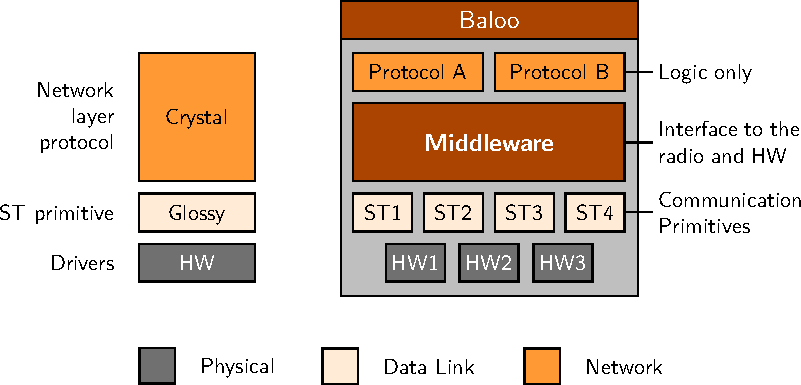
\includegraphics[scale=1]{stack_baloo.pdf}\\~\\
  \begin{minipage}[t]{.47\linewidth}
    \textbf{(a)} The implementation of the network layer protocol (Crystal) couples the interface to the underlying \ST primitive (Glossy) and the protocol logic, \ie how long are the communication rounds, which radio channel is used, \etc
  \end{minipage}
  \hfill
  \begin{minipage}[t]{.47\linewidth}
    \textbf{(b)} Thanks to its additional middleware layer, \baloo flexibly supports multiple \ST primitives and significantly reduces the efforts required to implement  network layer protocols compared to traditional stacks, like LWB~\cite{ferrari2012LWB} or Crystal~\cite{istomin2018Interferenceresilient}.
  \end{minipage}
  %
  \caption{Crystal~\cite{istomin2018Interferenceresilient} is a typical example of network stack based on \ST (\cref{fig:stack_baloo}a).
		Conversely, \baloo is a flexible design framework.
		It is based on a middleware layer that separates the concern of timely execution of \ST primitives from the implementation of the protocol logic (\cref{fig:stack_baloo}b).}
	\label{fig:stack_baloo}
\end{figure}

This chapter \emph{is not} meant to cover all details and inner mechanisms of \baloo, but mainly presents the core concepts of the framework.
\baloo is open source and the complete technical documentation is available online~(\cref{append:baloo_artifacts}).

% !TEX root = ../00_thesis.tex

\section{Overview of \baloo}
\label{sec:baloo_overview}

This section presents an overview of the concepts of \baloo. The implementation of these concepts using a middleware will be described in the next section (\cref{sec:baloo_implementation}).

%[here a one sentence summary of Baloo and its concepts, which are then justified]
\baloo is a flexible framework designed to harness the potential of the Synchronous Transmissions (\ST) technology and make it more accessible.
\baloo uses Time Division Multiple Access (TDMA) rounds made of communication slots. A \ST primitive is executed in each slot.
All necessarily control information is sent by a central node in the first slot of each round.
The core of \baloo is made of a middleware layer (see \cref{fig:stack_baloo}) which isolates the network layer from the lower layers. Concretely, this separates the management of the radio and timer settings from the implementation of the protocol logic.

\fakeparQM{Why Synchronous Transmissions}
As discussed in \cref{sec:baloo_intro}, \ST is a wireless communication technique known to be reliable, fast, and energy efficient.
%
\ST primitives communicate using so-called \textsl{floods}, which realize an any-to-all communication. Thus, \ST seamlessly supports multiple types of transmission patterns (\ie unicast, multicast, broadcast).
As a result, \ST enables to abstract away the complexity of a multi-hop mesh into a \textsl{virtual single-hop network}.
%
Furthermore, some \ST primitives (\eg Glossy~\cite{ferrari2011Glossy} or Robust Flooding~\cite{lim2017Competition}) provide tight bounds on the completion time of a flood, given the payload size and network diameter.

This makes \ST particularly suited for a time-triggered communication scheme. Within one bounded time slot, one can schedule a communication from one to any (set of) node(s) in the network, which greatly simplifies the design of a network layer protocol.

\baloo uses Glossy~\cite{ferrari2011Glossy} as default \ST primitive, but it also supports other primitives, \eg Chaos~\cite{landsiedel2013Chaos}. In principle, \baloo is compatible with arbitrarily many other primitives (see \cref{subsec:multi-ST-primitives}), thus addressing \feature{Versatility}.

\squarepar{%
	\fakepar{Round-based Design}
	To maximize the benefits of \ST, \baloo organizes communication in
	TDMA rounds, with dedicated time slots assigned to specific nodes which are then allowed to initiate a transmission in this slot.
	The first slot in each round is assigned to a central node, called the \textsl{host}, to send some control information (see below). This \textsl{control slot} is then followed by arbitrarily many \textsl{data slots}.
	Nodes turn their radio off between rounds to save energy.

	While this framework may look restrictive and hinder \feature{Generality}, such round-based design is in fact very generic, and compatible with many (if not all) \ST-based network stacks proposed so far in the literature. The flexibility and limitations of \baloo will be discussed in the evaluation (\cref{sec:baloo_eval,sec:requirements}).%
}

\fakepar{Control Information}
In \baloo, the control packet, sent at the beginning of each round, plays a key role. It is constructed such that if a node receives a control packet from the host, this nodes knows exactly\\
	\inlineitem how to execute the current communication round, and\\
	\inlineitem when to wake up for the next round.\\
Thus, the control packet contains both \textsl{schedule information} (\eg the slot assignment for the round or the time interval before the next round) and \textsl{configuration parameters}, like the length of the slots or the number of retransmissions.
The control packet is broadcast using Glossy~\cite{ferrari2011Glossy}, which is also used to synchronize the whole network.

\baloo is very flexible (\feature{Usability}, \feature{Generality}); both schedule and configuration can be updated at anytime by the host and the whole network adapts to follow the instructions.
This poses the problem of a node not correctly decoding a control packet, thus having possibly outdated control information.

Consequently, \baloo adopts the following fail-safe mechanism: \textsl{a node does not participates in a communication round unless it correctly decodes the control packet}. This guarantees that, even in case of packet losses, a node will never disturb the execution of the rest of the network.

\fakepar{A Middleware to Provide the Right Level of Abstraction}
The main challenge in the design of \baloo is the definition of an interface that isolates the management of the radio (\ie running the \ST communication primitives) from the implementation of the protocol logic at the network layer.
%
{
\setlength{\parskip}{3pt}%
\setlength{\parsep}{3pt}%
\baloo realizes this interface using a middleware layer that is responsible for the following tasks:
\begin{itemize}

	\item The middleware organizes the timers and controls the radio operations (\ie it executes the \ST primitives).

	\item The middleware manages the communication round operations according to the control information received from the host.

	\item The middleware executes callback functions, which are used to interact with the application running above the network layer (\ie passing packet payload and implementing the protocol logic).

\end{itemize}
The middleware is a \textsl{fixed piece of software} which can be configured but neither accessed nor modified by the network layer.
The protocol logic (payload management, state keeping, \etc) is implemented entirely within the callback functions~(\cref{subsec:CB}).%
The middleware interface is illustrated in \cref{fig:callbacks}.%
}

With this approach, all low-level programming complexities are managed by the middleware and let the network designer focus on the main task: design the protocol logic of the network layer.

These concepts form the core of \baloo and address the \feature{Usability}, \feature{Generality},  and \feature{Versatility} requirements of a flexible network stack design.
Additional concepts are required to ensure that the timing requirements of \ST are met (\feature{Synchronicity}): this is the focus of the next section.

% !TEX root = ../00_thesis.tex
\section{Implementing the Concepts}
\label{sec:baloo_implementation}

\begin{figure}
	\centering
	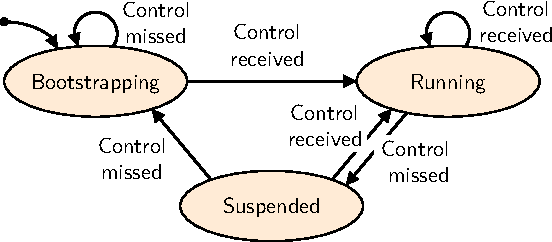
\includegraphics[scale=1]{state-machine}
	\caption{The middleware in \baloo implements a minimal state machine, sufficient to capture the desired behaviour of a node at physical layer.
		\capt{A node either executes normally (\textsl{Running}), stays synchronized but does not participate to the communication rounds (\textsl{Suspended}), or continuously listens for an incoming control packet (\textsl{Bootstrapping}).}}
	\label{fig:state-machine}
	\vspace{-0.5cm}
\end{figure}

The previous section described the general concepts of \baloo.
% , and discussed how they meet challenges \chal{1}-\chal{3}, presented in the Introduction.
In this section, we present how we implemented these concepts to meet the \feature{Synchronicity} requirement and complete the design of \baloo.

\subsection{Contiki as Operating System}
\label{subsec:contiki}


\baloo relies on the availability of \ST primitives (\eg Glossy~\cite{ferrari2011Glossy}, Chaos~\cite{landsiedel2013Chaos}, \etc). Most openly available primitives use Contiki~\cite{dunkels2004Contiki} as the underlying operating system, which made Contiki an obvious choice to implement \baloo.
We have ported these primitives to the new version of the OS: Contiki-NG~\cite{ContikiNG}.%
\footnote{v4.2, released in November 2018}

Contiki is a cooperative multi-threaded OS, tailored for resource-constrained devices in the Internet of Things.
The middleware layer is implemented as the ``master'' protothread~\cite{dunkels2006Protothreads}, where most of the program is executed. The middleware implements the communication rounds, controls the radio operations, and executes the callback functions in which the network protocol logic is implemented (see \cref{subsec:CB}).


\subsection{Minimal State Machine}
\label{subsec:state-machine}
For generality and simplicity, the middleware implements only a minimal state machine. A node is either in \textsl{Bootstrapping}, \textsl{Suspended}, or \textsl{Running} state.
State transitions result from (un)successful receptions of control packets (see \cref{fig:state-machine}).
When bootstrapping, a node continuously listens for a control packet. In the \textsl{Suspended} state, a node does not participate in the round and will sleep until the next round.

As described in \cref{sec:baloo_overview}, a node may participate in a round (\ie be in the \textsl{Running} state) if and only if it correctly receives the control packet at the beginning of the round.
%
The default behaviour of \baloo is that a node suspends itself if it misses a control packet, and goes back to Bootstrapping if it misses two in a row. A node exits the \textsl{Bootstrapping} state whenever it receives a control packet containing both scheduling and configuration information, \ie when a node knows with certainty how it is expected to operate.
%
If necessary, the network layer protocol can extend this minimal state machine using one of the callback functions (see \cref{subsec:add_func}).

\subsection{Middleware Callback Functions}
\label{subsec:CB}

\squarepar{%
	\baloo uses callback functions to implement the network layer protocol logic. This is how the network layer interacts with the middleware at runtime (\feature{Usability}).
	There are five different callbacks, each having a specific purpose and executed by the middleware at precise points in time~(\cref{fig:callbacks}).%
}

\begin{functions}

	\item[on\_control\_slot\_post()]~\newline
	is executed at the end of the control slot.
	It is used to process the received control information and prepare for the round.

	\item[on\_slot\_pre()]~\newline
	is executed before each data slot.
	It is used to pass the payload to send to the middleware, if any.

	\item[on\_slot\_post()]~\newline
	is executed at the end of each data slot.
	It is used to process the received payload, if any.

	\item[on\_round\_finished()]~\\
	is executed at the end of the round.
	It is used to do more time consuming state management or data processing.

	\item[on\_bootstrap\_timeout()]~\newline
	is executed when a node fails to bootstrap (\ie it has listened for some time without receiving any control packet).
	This callback allows nodes to go to sleep and retry bootstrapping later, in order to save energy.

\end{functions}

\squarepar{%
	These callback functions are also used to implement more advanced features of \baloo (\eg skipping a slot), which are briefly presented in \cref{sec:adv_features}.%
}

\afterpage{
	\begin{landscape}
		\begin{figure*}
			\centering
			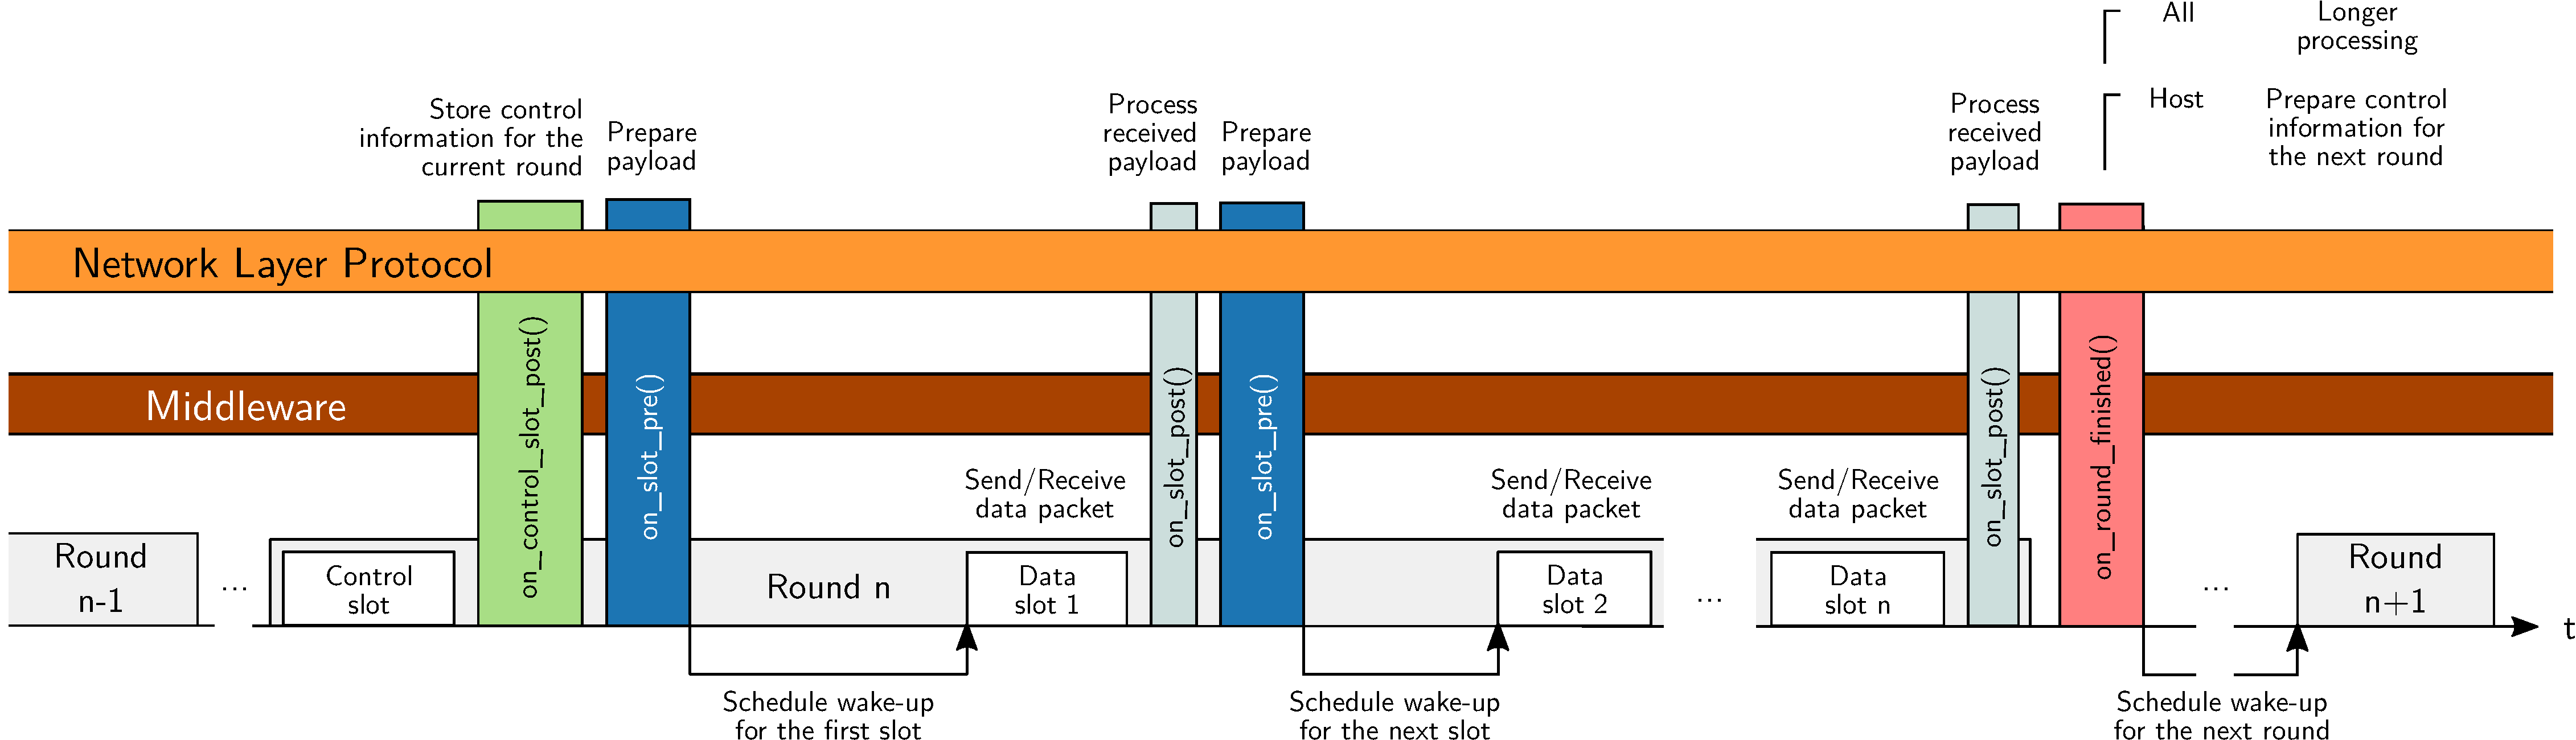
\includegraphics[width = \linewidth]{callbacks}
			\caption{The protocol logic, \ie the handling of application payloads and the definition of the desired control parameters, is implemented in callback functions. These callbacks are triggered by the middleware before and after each slot and at the end of a round.
				The middleware schedules the wake-up of the radio core and executes the \ST primitives.}
			\label{fig:callbacks}
		\end{figure*}
	\end{landscape}
}


\subsection{Achieving Timeliness of Execution}
\label{subsec:timeliness}

\squarepar{%
	The callback functions enable flexible interactions between the network layer and the middleware. While this is key to address \feature{Usability} and \feature{Generality}, it also inherently couples the two software components, thus challenging the timely execution of the middleware and compromising \feature{Synchronicity}.%
}

Indeed, the callbacks execute between communication slots or between rounds (see \cref{fig:callbacks}), which must start synchronously on all nodes to permit successful \ST.
The middleware could interrupt an overrunning callback to ensure synchronicity, but that is not desirable. In general, an interrupted callback would have to be considered as a failure by the network layer; then successful \ST at the lower layer would not really matter anyway.

\squarepar{%
	To mitigate this problem, the middleware \textsl{monitors} the execution time of the callbacks. If a callback overruns and the middleware cannot guarantee the timely execution of the next slot, this slot is skipped (\ie the node does not participate in this slot) and a notification event is sent to the network layer.%
}

With this approach, \baloo can guarantee to respect the timing requirement for \ST \textit{under the condition that the callbacks have enough time to complete their execution}.%
\footnote{This default strategy may lead to a starvation problem if a callback ``never'' returns, \eg if it relies on another software sitting at higher layers. One advanced feature lets the middleware interrupt overrunning callbacks (see \cref{subsec:add_func}).}
To satisfy this condition, the available time between slots for the execution of the callbacks is controlled by a dedicated configuration parameter: the \textsl{gap time}.
Since callbacks implement the network layer protocol logic, it can only be the responsibility of the network designer to set suitable gap times such that the \feature{Synchronicity} requirement is met.
Guidelines for setting such parameters (and in general: how-to use \baloo) are part of the online documentation~(\cref{append:baloo_artifacts}).
\subsection{Supporting Multiple \ST Primitives}
\label{subsec:multi-ST-primitives}

Compared to previously proposed low-power network stacks, one key difference of \baloo is that it flexibly supports multiple \ST primitives (\feature{Versatility}).
This is difficult given the nature of \ST, which requires tight timing of radio events (from sub-\us to tens of \us depending on the primitive~\cite{yuan2013LetTalkTogether}).

In practice, achieving such synchronization requires a direct monitoring of hardware timers and a custom implementation of the associated Interrupt Service Routines (ISR) for each \ST primitive executed by the middleware in \baloo.
However, there cannot be multiple implementation of the same ISR. Thus, supporting multiple \ST primitives in the same stack requires to extract the interrupt management from the \ST code, which becomes a shared software component between different primitives.

Technically, we implemented this using a renaming trick. Indeed, each \ST primitive has its own ISR implementation for the radio timer, but \baloo never uses more than one \ST primitive at the same time (\ie one per data slot). The middleware must only execute the instructions of the ISR from the currently running primitive.
Thus, we can encapsulate the ISR of each primitive into a dedicated (\ie unique)  function and implement the radio timer ISR as a simple ``switch'' function. A global variable keeps track of the currently running primitive; whenever the radio timer fires, the corresponding primitive ``ISR function'' is executed.

The only difference with the original primitives' implementation is an additional software delay between the radio interrupt and the execution of the ISR's instructions (the few ticks of delay to execute the switch).
This adds a negligible synchronization error due to differences in clock speed across different nodes.%
\footnote{%
	Assuming an absolute clock drift of 100\ppm between two nodes (which is pessimistic), the error introduced is $\sim 0.24$ picosecond per tick of delay.
	}

Using this approach, \baloo currently supports two \ST primitives, Glossy~\cite{ferrari2011Glossy} and Chaos~\cite{landsiedel2013Chaos}, as well as a classical strobing communication primitive: one node transmits its packet, multiple times, while all other nodes only listen.
Practically, there is no limitation on the number of primitives that \baloo can support, apart from the available memory.

% !TEX root = ../00_thesis.tex

\section{Advanced Functionalities}
\label{sec:adv_features}

In \cref{sec:baloo_overview} and \ref{sec:baloo_implementation} we presented the general concepts of \baloo and how we implemented them to meet the requirements presented in \cref{sec:baloo_intro}.
To further extend the variety of network layer protocols that can be implemented using \baloo, we have enriched the framework with various features, most of which have been used in previous protocols and proved themselves useful.
We briefly present these features in this section.

\subsection{High-level Functions}

\label{subsec:add_func}

\begin{description}

	\item [Detection of interference]
	Low-power wireless networks often suffer from interference.
	Multiple strategies have been proposed to escape and/or mitigate its effects.

	\baloo allows to monitor the power level on the channel being used during a slot. This information can be used to detect potential interference and react accordingly.

	This feature is used \eg in Crystal~\cite{istomin2018Interferenceresilient}.

	\item [Advanced state machine]
	The middleware in \baloo implements a minimal but sufficient state machine composed of three states (\textsl{Running}, \textsl{Suspended}, \textsl{Bootstrapping}; see \cref{subsec:state-machine} and \cref{fig:state-machine}).

	\baloo lets the network layer protocol implement a more advanced state machine. The return value of the \texttt{on\_control\_slot\_post()} callback is used to inform the middleware of the desired behaviour for the node, \ie whether it should be in the  \textsl{Running}, \textsl{Suspended}, or \textsl{Bootstrapping} state for the coming round.

	This feature is used \eg in LWB~\cite{ferrari2012LWB}.

	\item[Starvation protection]
	Skipping slots due to overrunning callbacks may lead to starvation problems. The middleware behaviour can be modified to interrupt these overruns.
	%
	If and when this occurs, the interrupted node will suspend its operation for the coming slot (or the complete round, in case the \texttt{on\_control\_slot\_post()} over-runs).

	At the time of writing, this feature is \textbf{not included} in the publicly available implementation of \baloo.

\end{description}

\subsection{Scheduling Features}

\label{subsec:adv_sched}

\begin{description}

	%scheduling
	\item[Contention slots]
	In a contention slot, all nodes are allowed to transmit their own packet; they ``contend'' for access to the wireless medium. The successful reception of one of the packets remains possible due to the capture effect~\cite{yuan2013LetTalkTogether}.

	Contention slots are used in many protocols, including LWB~\cite{ferrari2012LWB} and Crystal~\cite{istomin2018Interferenceresilient}.

	\item [Per-slot configuration]
	By default, the same configuration parameters are used for all slots in the same round. \baloo lets the network layer specify some configuration on a per-slot basis. These optional parameters are sent by the host as part of the control packet.

	Crystal~\cite{istomin2018Interferenceresilient} for example uses different number of retransmissions for data and acknowledgement packets (the latter are retransmitted more often).

	\item [Static schedule and configuration]
	In many network layer protocols, the scheduling policy is static: either the control information remains the same or it changes according to some offline algorithm.

	In such cases, \baloo can spare the overhead of sending redundant information in the control packet, thus saving time and energy. All nodes are then responsible to locally update their control information.

	Static schedules are used \eg in TTW~\cite{jacob2017TTW_extended} or Crystal~\cite{istomin2018Interferenceresilient}.

	\item [Skipping slots and rounds]
	It is sometimes useful that some nodes do not participate in certain slots, or even skip complete rounds, \eg to save energy, or to improve performance in very dense networks.

	\baloo lets the network layer trigger slot skipping using the return value of the \texttt{on\_slot\_pre()} callback.
	To skip an entire round, one can return \textsl{Suspended} in the \texttt{on\_control\_slot\_post()} callback (see \cref{subsec:add_func}).

	This feature is used \eg in Sleeping Beauty~\cite{sarkar2016Sleeping}.

	\item [Repeating slots or rounds]
	On the contrary, it may be useful to repeat the execution of specific slots, or even entire communication rounds (\eg when the number of slots required in a round is dynamic) or to retransmit lost packets.

	\baloo lets the network layer trigger slot and round repeat using the return value of the \texttt{on\_slot\_post()} callback.\\
	% \begin{subitemize}
		% \item
		\inlineitem
		If the slot repeat flag is received, the same slot is re-executed.\\
		% \item
		\inlineitem
		If the round repeat flag is received, the middleware immediately restarts executing from the first slot of the round.\\
	% \end{subitemize}
	This feature is used \eg in Crystal~\cite{istomin2018Interferenceresilient}.


\end{description}

\subsection{Radio Settings}
\label{subsec:adv_radio}


\begin{description}
	%radio parameters
	\item [Radio channel setting]
	\baloo lets the network designer select the radio frequency channel for each slot. This can be useful to proactively or reactively hop between channels in case of interference.

	This feature is used \eg in Crystal~\cite{istomin2018Interferenceresilient}.

	\item [Transmit power setting]
	\baloo lets the network designer set the desired transmit power, possibly changing between each communication slot.

\end{description}

% !TEX root = ../00_thesis.tex

\section{Performance Evaluation}
\label{sec:baloo_eval}

% We presented \baloo, a flexible design framework for low-power network stacks based on \ST; we now evaluate our proposal.
This section presents an evaluation of \baloo.
We look first into qualitative aspects. We argue that \baloo is indeed usable and validate the premise that it makes it easy to design a network stack based on \ST.
We then discuss quantitative aspects by looking at the performance overhead of using \baloo compared to original implementations.

\subsection{Qualitative Evaluation}
\label{subsec:usability}

%Evaluating the usability of a software or tool is complex.
The evaluation of software usability is a challenging task that suffers from almost unavoidable bias.
To support our claim that \baloo is indeed easy to use, we used it ourselves to perform one of the most time consuming task in experimental research: the re-implementation of someone else's protocol.
%We chose three: SB, Crystal and LWB. Why?
%- They are well-known solutions
%- They cover most of the features offered by \baloo
%- The original code is available
We re-implemented the protocol logic of three network stacks: Crystal~\cite{istomin2018Interferenceresilient}, Sleeping Beauty~\cite{sarkar2016Sleeping}, and LWB~\cite{ferrari2012LWB}. We chose these protocols because:
\begin{itemize}

	\item They are well-known solutions from the literature, considering different types of scenario.

	\item Together, they use most of the features offered by \baloo.

	\item The authors' source code is publicly available.

\end{itemize}


It is fair to say that the fact that {we} can use {our} own software brings only little evidence of the usability of \baloo.
Indeed, its usability will be ultimately demonstrated if and when other people start using it to implement their own protocols.
%To support that:
%- code is available, with an extensive documentation of the various features and how to use them
%- our re-implementations of known protocols are provided
%- test applications showcasing the various features
To facilitate this, the code of \baloo is openly available, including demo applications, and is accompanied by a detailed documentation of its features and how to use them.
Naturally, our re-implementations of Crystal, Sleeping Beauty, and LWB are also available~(\cref{append:baloo_artifacts}).

In addition, we used the 2019 EWSN Dependability Competition~\cite{DepComp2019} as a case study.
In this competition, networking solutions must perform well across a wide range of input parameters (\eg data rates or payload sizes), which demands the network stack to be adaptive.
This is a perfect application for \baloo: by design, the middleware takes care of adjusting the timing of operations (\ie when the \ST primitives should be executed) based on the application parameters (\eg the payload size).
%
Furthermore, one can leverage the availability of different primitives. For example, after a data packet has been sent using Glossy~\cite{ferrari2011Glossy}, one can efficiently collect acknowledgements from all destinations using Chaos~\cite{landsiedel2013Chaos}.

We tested the \feature{Usability} of \baloo by having master students (who did not have any prior knowledge of \baloo, nor \ST) competing using the framework~\cite{mueller2019Competition}.
Naturally, they did not beat teams of experienced researchers, but they did perform well.
As they put it themselves in their report:
\begin{quote}
	``We had not much prior experience in WSN protocol design. While the result is not perfect, we managed implement our protocol within 8 weeks of part-time work. We would not have been able to do that without \baloo.''~\cite{schaper2019LowPower,mueller2019Lowpower}
\end{quote}



Finally, another important qualitative aspect of \baloo is its portability. The underlying middleware has been designed to minimize the software parts that are platform-dependent, and those have been isolated as much as possible.
Essentially, the platform-dependent part is limited to the hardware timer interface and the radio drivers (further discussed in \cref{sec:requirements}).
%
\baloo is readily available on two platforms, the CC430 SoC~\cite{CC430F6137} and the TelosB mote~\cite{TelosB}.
Thanks to the abstraction provided by the middleware, the network layer protocol implementations using \baloo are \textsl{platform agnostic}. In other words, the same network layer implementation can be used to compile binaries for any platform supported by \baloo.
%
We argue that these elements, altogether, show the usability of \baloo.

\subsection{Quantitative Evaluation}
\label{subsec:overhead}

Abstraction and flexibility usually impact quantitative performance metrics.
In this section, we evaluate the performance overhead of \baloo along four metrics: the packet reception rate (PRR), the radio duty cycle (DC), the binary size, and the number of lines of code.

%Description of the objective: validate that \baloo `works', and quantifying the overhead. Not about the performance evaluation of the network layer protocols themselves.
%$->$ thus only limited tests on a single testbed.
We performed this evaluation using our three re-implementations of Crystal~\cite{istomin2018Interferenceresilient}, Sleeping Beauty~\cite{sarkar2016Sleeping}, and LWB~\cite{ferrari2012LWB}.
It is important to clarify the objective of the experiments we conducted: the goal is to evaluate the \textsl{performance overhead} of using \baloo compared to native implementations; not to evaluate the actual protocol performances.

\fakepar{Experimental Setup} All our experiments were conducted on Flocklab~\cite{lim2013FlockLab} as it is the only public testbed featuring both CC430 SoC~\cite{CC430F6137} and TelosB motes~\cite{TelosB}, the two platforms for which \baloo is available.
All tests ran for one hour on 26 nodes, leading to tens of thousand data packets exchanged for each protocol.
As much as possible, we designed the experiments to match those from the original protocol papers~\cite{istomin2018Interferenceresilient,sarkar2016Sleeping,ferrari2012LWB}.
\begin{description}

	\item[Crystal]
	We ran tests varying the number of source nodes $U$ that have a packet to transmit in each round.
	We used $U = \{0,1,20\}$. All other parameters were set according to the author's paper (first row of Table 2 in ~\cite{istomin2018Interferenceresilient}).

	\item[Sleeping Beauty]
	We ran tests varying the percentage of nodes that that have a packet to transmit in each round.
	We used $12.5\%$, $25\%$, and $50\%$ of the available nodes.
	All other parameters were set according to the author's paper~\cite{sarkar2016Sleeping}.

	\item[LWB]
	We ran tests varying the inter-packet interval $IPI$ of the data stream registered by each node in the network.
	We used $IPI = \{4\s, 30\s\}$ and the dynamic scheduler aiming to minimize energy consumption.

\end{description}


In each case, we compared: \emph{(i)} the results reported in the original papers, \emph{(ii)} the results we obtained by running the publicly available code, and \emph{(iii)} our re-implementations using \baloo on both the TelosB motes and \emph{(iv)} the CC430 SoC.
All results are summarized in Tables \ref{table:PRR} to \ref{table:LoC}. Before discussing each metrics in details, some comments are useful.
\begin{itemize}

	\item
	Although the original code of Sleeping Beauty is openly available~\cite{Code_SleepingBeauty}, we failed to run the protocol successfully. More precisely, the observed behaviour was quite different from the paper description and led to inexplicably poor results.
	It did not seem fair to present these as a truthful measure of the protocol performance.
	Thus, we do not report any results for the native code for Sleeping Beauty.

	\item
	The original Sleeping Beauty paper does not report exact values for PRR and duty cycle. The values from Table \ref{table:PRR} and \ref{table:DC} were read from Fig.~9 in ~\cite{sarkar2016Sleeping}.

	\item
	The original LWB paper presents results from an implementation on TelosB, but the available code from the authors is for the CC430 SoC~\cite{Code_LWB}.
	Thus, we compare our re-implementations with the native code, but not with the original paper results.

\end{itemize}

\afterpage{
	\begin{landscape}
		\begin{table*}
			\centering
			\caption{\raggedright End-to-end packet reception rate (PRR), expressed in percentage (\%)}
			{\smaller\input{\PathTab/PRR.csv}}
			\label{table:PRR}
		\end{table*}
		\vfill
		\begin{table*}
			\centering
			\caption{Average radio duty cycle (DC) across all nodes but the data sink, expressed in percentages (\%)\newline
			\capt{For Sleeping Beauty, the reported values exclude the bootstrapping phase.}}
			{\smaller\input{\PathTab/DC.csv}}
			\label{table:DC}
		\end{table*}
		\vfill
		\begin{table}
			\parbox{.45\linewidth}{%
				\caption{Estimate of the binary size of the network layer protocol code (in\kb)}
				{\smaller\input{\PathTab/Binary.csv}}
				\label{table:Binary}
			}
			\hfill
			\parbox{.45\linewidth}{%
				\caption{Estimate of the number of lines of code in the implementation of the network layer protocol}
				{\smaller\input{\PathTab/LoC.csv}}
				\label{table:LoC}
			}
		\end{table}
	\end{landscape}
}

\fakepar{Packet Reception Rate (PRR)}
We consider the end-to-end PRR: the percentage of the packets generated by the application at the source nodes that have reached their intended destination.
We count a packet as lost \textsl{only if none of its transmissions} has been successfully received at the destination. In Crystal~\cite{istomin2018Interferenceresilient} for example, data packets may be lost and successfully received later; that does not impact the PRR.

We do not expect any overhead in term of reliability from using \baloo, as this metric essentially depends on the underlying \ST primitive and the network layer protocol logic; two elements not modified by the framework.
This metric mostly verifies that our re-implementations ``work''.
The results in Table~\ref{table:PRR} indeed show similiar PRR for all implementations, with one notable exception.

\baloo on CC430 for Crystal with $U=20$ performs poorly. After closer investigation, it appears that the success rate of the capture effect on the CC430 SoC is much lower than on the TelosB (presumably due to the different modulation schemes used by the radio: 2-FSK and O-QPSK respectively).
When $U=20$, it is highly probable that all the one-hop neighbours of the sink are selected source nodes that generate a packet in a round (20 out of 25 nodes available on Flocklab).
As Crystal transmits all its data packets using contention slots,%
\footnote{Successful contention slots rely on capture effect, see \cref{sec:adv_features}}
the sink only rarely receives packets in these rounds, thus resulting in poor PRR.

\fakepar{Radio Duty Cycle (DC)}
The radio duty cycle (DC) is expected to reveal more of the actual overhead induced by \baloo. Our results are summarized in Table~\ref{table:DC}.

The LWB experiment perfectly matches our expectations: the DC are comparable, with a slight increase for \baloo (5 to 15\% more compared to the native code), which is due to the cost of sending more information in the control packet.

In the original \baloo paper~\cite{jacob2019Baloo}, we reported surprising results regarding Crystal: Our results on the same platform (TelosB) showed significantly higher DC both for the native code and our re-implementation (from 50\% to 100\% increase) whereas on the CC430 SoC, results are more comparable.
This was due to a misconfiguration of the clear channel assessment (CCA) threshold value: there is an offset of approximately $45dB$ between the value set in the register and the actual sensitivity of the CCA pin.%
\footnote{\cite{cc2420_datasheet}: RSSI / Energy Detection, page 48}
%
Consequently, when setting $-60\dBm$ (the value suggested by the Crystal authors~\cite{istomin2018Interferenceresilient}), we actually obtained a CCA sensitivity of about $-105\dBm$, which is lower than the noise floor. Hence, Crystal consistently detected possible interference and (often needlessly) prolonged the communication rounds, thus artificially increasing the DC.
We have re-run these experiments with the correct CCA setting (\ie $-60\dBm$) and validate that, as expected, the DC is slightly increased by \baloo~(\cref{table:DC}).

The results for Sleeping Beauty are more surprising. In spite of the overhead induced by \baloo, our re-implementation achieves about $2.5$x reduction in DC. It is unclear what can be the source of such difference.
As we based our re-implementation only on the original paper description~\cite{sarkar2016Sleeping}, one possible explanation is that we might lack some of the original protocol features, that would induce more radio on time.
However, the good results we obtain with our re-implementation would question the usefulness of such features.
% This remains an open question.

\fakepar{Binary size}
The binary file size is another metric where we expect \baloo to induce some overhead, as the middleware introduces additional files, types and features that are not always necessary for all protocols.

Since the protocol implementations we looked at are based on different versions of the Contiki OS, we tried to evaluate the actual size of the \textsl{network layer protocol} only by deducing the memory required for the OS. The OS memory requirements were obtained by looking at the size of a minimal ``hello-world'' application. Table~\ref{table:Binary} reports the difference between the total and ``hello-world'' binary sizes, a rough \textsl{estimate} of the memory required by the network layer protocol implementation.%
\footnote{%
More advanced metrics could be used, \eg summing the size of relevant functions in the object file. We chose to used a very simple approach because our goal is only to give an estimate of the impact of \baloo on the memory requirements.}

Actually, the memory size of our re-implementations is comparable to that of the native codes. Likely, t	his is due to the configurable nature of the framework. Many features are available, but the protocol designer flexibly selects which are required, thus limiting the size of the compiled code.
Furthermore, the structure imposed by the framework may lead to a more concise implementation, as discussed next.

\fakepar{Lines of Code}
The last metric we considered is the number of lines of code that is part of the \emph{network layer protocol} (\ie for the \baloo re-implementations, only the callbacks and custom functions; not the middleware code).
This is arguably a rough metric, for at least two reasons: \emph{(i)} none of the implementations aimed to minimise its code size; \emph{(ii)} in the original implementations, it is not easy to isolate the code implementing the protocol logic from the interface with the lower layers (precisely, this is one of the differences with \baloo).
Still, the number of lines of code provides some insights on the potential benefits of \baloo in terms of usability.

The results in Table~\ref{table:LoC} show that using \baloo can significantly reduce the amount of code required to implement some network layer protocol logic (up to 45\% reduction for LWB).
More importantly, the protocol implementations in \baloo \textsl{do not contain} any timer setting or register accesses, as these are handled directly by the middleware.

\fakepar{Summary}
Ultimately, our quantitative evaluation shows through a few examples that implementations using \baloo perform well and that the framework induces only limited (if any) overhead in terms of radio duty cycle and binary size.

% !TEX root = ../00_thesis.tex
\vspace{-1cm}
\section{Discussion and Limitations}
\label{sec:requirements}

\squarepar{%
	We argued that \baloo is a usable, flexible, and performant design framework (\cref{sec:baloo_eval}).
	To complete the description, we now detail hardware and software requirements and discuss the portability and limitations of the framework.%
}

\subsection{Requirements}
\label{subsec:requirements}
\fakepar{Hardware requirements}
The only strict hardware requirement of \baloo is one dedicated Capture Compare Register (as required by any time-triggered protocol). The actual timer frequency is not important; a standard 32\kHz clock is already fast enough.
This timer is used to schedule the communication slots, wake-up times, and callback executions.

Both supported platforms feature an MSP430 CPU, but this is not a constraint. An ARM core like the ones embedded on the nRF52840~\cite{nRF52840} or the OpenMoteB~\cite{OpenMoteB} platforms would work as well. It would eventually be even more flexible given the support for interrupt priorities.

\fakepar{Software requirements}
\baloo requires a software-extended timer implementation to enable the scheduling of firing epochs further than one roll-over of the timer. This is (surprisingly) not part of Contiki by default, but it is a rather minor extension.
%
Some features of \baloo rely on radio functions (\eg the noise detection); these features are obviously platform-dependent.
%
The rest of the platform-dependent software in \baloo is a mapping between \ST primitive functions and generic macros used by the middleware.

\subsection{Portability}
\baloo itself has limited hardware and software requirements (\cref{subsec:requirements}). The main constraint comes from the availability of \ST primitives, which are notoriously difficult to implement; but this is independent of the framework.
Assuming \ST primitives are available, the requirements and efforts to port \baloo to a new platform are limited.
%A guide on ``how-to-port'' \baloo is included in the documentation ~\cite{Baloo}.

We implemented \baloo using Contiki (see \cref{sec:baloo_implementation}), which turned out having pros and cons. On the one hand, it facilitates the port of \baloo to other platforms \emph{that already run Contiki}.
On the other hands, it makes \baloo harder to port to \emph{other platforms}, as it requires to port the Contiki OS first. It has been a limitation in some later projects (see \cref{sec:outcomes}).

Furthermore, \baloo does not require much of the complex machinery of a full-fledge operating system. Thus, a bare-metal implementation of \baloo could bring multiple benefits: increased reliability (as there is no interference from the OS), lighter weight, and simpler to port on any platform (as there is no need to port an entire OS first).

\squarepar{%
	At the time of writing, the only known publicly available implementation of \baloo uses Contiki. Ongoing development efforts are discussed in \cref{sec:outcomes}.%
}

\subsection{Limitations}

\baloo is a framework that facilitates the design of \ST-based network stacks by providing some level of abstraction.
We showed in \cref{sec:baloo_eval} that this abstraction has only a moderate impact on performance.
However, abstraction also limits the design freedom, and this also applies to \baloo. We honestly tried to think of sensible design concepts that are incompatible with the framework, while they would be technically possible to implement:
\begin{itemize}
	\item \baloo does not support multiple hosts (\eg for redundancy purposes).
	\item \baloo cannot start primitives at different times on different nodes (\eg to save energy).
	\item \baloo cannot execute different \ST primitives on different nodes during the same data slots.
\end{itemize}

\cref{sec:adv_features} presented a set of features offered by the \baloo framework. The feature set may not be complete, but (i)~it already offers a lot of options, and (ii)~it can be extended in the future, if necessary.
To the best of our knowledge, to date,
there is no \ST-based network layer protocol in the literature that is incompatible with \baloo. Likely, this is because what \baloo cannot do is either hard to do in general (\eg supporting redundant hosts) or are complex optimizations with uncertain benefits (\eg starting primitives with time offsets).

\subsection{Lessons Learned}
\label{sec:lessonsLearned}

\squarepar{During this work, we have learned a few lessons that might be worth sharing.}

\begin{description}

	\item[Re-implementing protocols.] Re-implementing a complete protocol (solely) based on the description from a research paper is very difficult, if not impossible. Many implementation details and design choices are omitted, for good reasons: research papers rather focus on novel concepts and ideas.
	Without a detailed technical documentation, a large part of the engineering is lost, and it becomes very hard to fairly compare two implementations of the same protocol.

	\item[Running protocols.] Publishing code does not mean it is (re)usable. Our experience with Sleeping Beauty has been a perfect example of that: even with the code freely available and quite some experience with testbed experiments, we were not able to successfully run the protocol on Flocklab.
	More generally usefulness of publishing code is greatly reduced (if not voided) without proper instructions and documentation.

\end{description}

\squarepar{%
	The point here is not to say that every research work \emph{must} openly release code together with an extensive documentation.
	However, \emph{if} one claims his or her research is providing practical solutions to concrete problems, then these solutions must be made available.
	When such a solution is a piece of software (\eg a network stack for low-power wireless), the (re)usability of the software is at least as important as the research paper presenting the underlying concepts.%
}

% !TEX root = ../00_thesis.tex

\section{Leveraging \baloo}
\label{sec:outcomes}

One important motivation for working on \baloo was to leverage the tool for our other research projects, and \baloo has proved itself useful indeed.
Within the time-frame of this thesis:
\begin{itemize}
  \item Master students used \baloo to participate in the 2019 EWSN Dependability Competition (\cref{subsec:usability}).
  \item We used \baloo to implement and test the Time-Triggered Wireless protocol~(\cref{ch:ttw}).
  \item We used \baloo to implement a generic firmware for collecting link quality data in wireless networks. We run this firmware on the FlockLab testbed multiple times per day and publish the newly collected data every month~\cite{jacobFlockLabLinkQuality}.
\end{itemize}

Contrarily to our original plans~\cite{jacob2019Baloo}, we decided not to pursue the integration of \baloo within Contiki-NG. The main reason is that \baloo barely uses any feature from the OS itself, which is more focused on offering standardized protocol implementations for the IPv6 stack. Ultimately, this hinders the portability of \baloo, as one needs to port the Contiki OS first.

The development of the \baloo framework continues. In middle-term, we plan a new release of the framework (including improved features related to Chaos~\cite{landsiedel2013Chaos}), a port to the SX1262 platform~\cite{semtechSX1262} using FreeRTOS~\cite{FreeRTOS}, and a bare-metal port to the nRF52840 platform~\cite{nRF52840}.
% Ideas of concrete research applications for \baloo are discussed in Conclusions~(\cref{ch:conclusions}).

% !TEX root = ../00_thesis.tex

\section{Related Work}
\label{sec:relwork}

\squarepar{%
  As mentioned in the introduction, the idea of middleware for Wireless Sensor Networks (WSN) has been around for more than a decade~\cite{romer2004Programming,chatzigiannakis200750,wang2008Middleware,mottola2012Middleware}.
  These papers generally agree on the needs and challenges for WSN middlewares.
  Yet, there have been relatively few proposals to address these challenges.
  Recent surveys~\cite{razzaque2016Middleware,onderwater2016overview} provide an overview of the middleware literature in the wider context of the Internet of Things, which covers all layers from local devices to cloud services.
  \cite{mottola2012Middleware} reviewed the literature focusing more on WSN:
  proposals include for example Impala~\cite{liu2003Impala} which explicitly address the problem of fault tolerance in mobile networks.
  Programming abstractions like TinyDB~\cite{madden2005TinyDB}, RUNES~\cite{costa2005RUNES}, or TinyLIME~\cite{costa2007Programming} have also been proposed.
  However, in these works, the level of abstraction is either higher or lower than the network layer.%
}

In the past two decades, countless wireless MAC protocols have been proposed (see \eg \cite{teleshermeto2017Scheduling,bartolomeu2016Survey} for recent surveys).
%
\cite{isolani2018Survey} surveyed and classified Wireless MAC protocols according to their programmability \emph{scope} (what elements of the MAC layer are programmable) and \emph{level} (the granularity at which the protocol logic can be programmed). The authors classify protocols as either monolithic, parametric or modular.
In the context of IEEE 802.15.4 networks, modular protocols include \eg the MAC Layer Architecture (MLA)~\cite{klues2007MLA} and $\lambda$-MAC~\cite{parker2010lambda}. In contrast, \baloo would be classified as parametric, as it allows ``parameter tuning through interfaces''.
Using Synchronous Transmissions (\ST) interestingly changes the way network stacks can or should be designed.
So far, only few network stacks using \ST have been proposed~\cite{ferrari2012LWB,istomin2018Interferenceresilient,sarkar2016Sleeping,sutton2017eLWB,jacob2017TTW_extended,suzuki2013Choco}, and almost no research has been conducted to propose a flexible design framework (\eg comparable to MLA~\cite{klues2007MLA}) but tailored to \ST.
Two noteworthy exceptions are A$^2$~\cite{alnahas2017a2} and Atomic-SDN~\cite{baddeley2019AtomicSDN}.

% A$^2$, a work with a very similar approach to ours.
A$^2$ aims to facilitate the design of \ST-based communication using a middleware component, called Synchrotron. However, A$^2$ is not a network stack, it is a \emph{generic \ST primitive}.
\baloo and A$^2$ actually complement each other perfectly:
\baloo facilitates the design of network layer protocols, but it requires to have \ST primitives (\eg Glossy~\cite{ferrari2011Glossy} or Chaos~\cite{landsiedel2013Chaos}) available, which are typically hard to implement.
In turn, A$^2$ facilitates the design of such \ST primitives.
The support of A$^2$ within \baloo would be a natural next step towards a fully flexible and configurable network stack based on \ST.

Atomic-SDN~\cite{baddeley2019AtomicSDN} is another work sharing this idea of a fully configurable network stack. \baloo and Atomic-SDN are very similar pieces of software, which have been developed in parallel.
Compared to \baloo, Atomic-SDN is slightly more specialized: it pre-defines top-level functions (collection, configuration, reaction, and association) with a given implementation, which the user can schedule on-demand. By contrast, \baloo leaves the user  access the various \ST primitives and compose them freely to implement the desired protocol logic.
Another key difference is precisely that \baloo lets the user pick-choose-and-combine the primitives to use, whereas Atomic-SDN is restricted to only one primitive (in the current implementation). Atomic-SDN uses a back-to-back transmissions schemes (\cite{baddeley2019Competition, lim2017Competition}) instead of traditional Glossy floods~\cite{ferrari2011Glossy}.

% !TEX root = ../00_thesis.tex

\section{Summary}

%What we presented
This chapter presented \baloo, a flexible design framework for low-power wireless network stacks based on \ST.
We illustrated its \feature{Usability} and \feature{Generality} by re-implementing three well-known network stacks: the Low-power Wireless Bus (LWB)~\cite{ferrari2012LWB}, Sleeping Beauty~\cite{sarkar2016Sleeping}, and Crystal~\cite{istomin2018Interferenceresilient}, and we showed that using \baloo induces only limited performance overhead in terms of radio duty cycle and memory usage.
\baloo supports the use of multiple \ST primitives within the same network stack (\feature{Versatility}) while guaranteeing that the timing requirements for \ST are met (\feature{Synchronicity}).

% Key concept/novel idea
The key concept of \baloo is its clean API, based on callback functions, which let the users focus on implementing the protocol logic without worrying about low-level radio control (interrupt handling, timer settings, \etc).
The API is generic and supports the different communication primitives. Through this API, multiple primitives can be used within the same network stack without additional complexity for the users.

% Take aways
The code of \baloo is openly available and is accompanied by a detailed documentation of its features and how to use them~(\cref{append:baloo_artifacts}).
Our re-implementations of Crystal, Sleeping Beauty, and LWB are also available.
We believe \baloo will be an important enabler for the development of future real-world applications leveraging state-of-the-art \ST technology.


% Chapter appendices
\begin{subappendices}
\newpage
% !TEX root = ../00_thesis.tex
\section{Appendix -- Artifacts and Links}
\label{append:baloo_artifacts}

\subsection{Related Publications}

\inlineRef%
{Synchronous Transmissions Made Easy: Design Your Network Stack with Baloo}%
{Romain Jacob, Jonas Bächli, Reto Da Forno, Lothar Thiele}%
{EWSN 2019. Beijung, China (February 2019)}

\customLink{\faFileTextO}{Paper}{10.3929/ethz-b-000324254}{https://doi.org/10.3929/ethz-b-000324254}
\customLink{\faDesktop}{Presentation}{10.3929/ethz-b-000328814}{https://doi.org/10.3929/ethz-b-000328814}

\inlineRef%
{Creating a Flexible Middleware for Low-Power Flooding Protocols}%
{Jonas Bächli}%
{Master Thesis. ETH Zurich (June 2018)}

\customLink{\faBook}{Thesis}{10.3929/ethz-b-000270388}{https://doi.org/10.3929/ethz-b-000270388}

\subsection{Complementary Materials}
Complementary materials for this chapters are available on GitHub, together with the dissertation source files. For all links below, replace\\
\linkroot  by ``{github.com/romain-jacob/doctoral-thesis/blob/master}''

\customLink{\faFilesO}{\tex sources}{\linkroot/30\_Baloo/}{\linkrootURL/30\_Baloo/}
\customLink{\faFileImageO}{Figures}{\linkroot/30\_Baloo/Figures/}{\linkrootURL/30\_Baloo/Figures/}
% \customLink{\faCopyright}{\credit}{\linkroot/credits/30\_Baloo.pdf}{\linkrootURL/credits/30\_Baloo.pdf}
\customLink{\faGlobe}{Webpage}{romainjacob.net/baloo}{http://www.romainjacob.net/research/projects/baloo/}
%
\customLink{\faCode}{\baloo source code}{}{}
  \customLink{}{--- Documentation}{GitHub Wiki}{https://github.com/ETHZ-TEC/Baloo/wiki}
  \customLink{}{--- Latest release}{10.5281/zenodo.3510171}{https://doi.org/10.5281/zenodo.3510171}
  \customLink{}{--- ``This-version'' release}{10.5281/zenodo.3530632}{https://doi.org/10.5281/zenodo.3530632}
\customLink{\faChain}{Experiment data}{}{}
  \customLink{}{--- Latest release}{10.5281/zenodo.3510198}{https://doi.org/10.5281/zenodo.3510198}
  \customLink{}{--- ``This-version'' release}{10.5281/zenodo.3510214}{https://doi.org/10.5281/zenodo.3510214}

\end{subappendices}

% ~
% \newpage
% ~
% \pagestyle{empty}
% ~
% \newpage
% ~
% \newpage

% !TEX root = ../00_thesis.tex

\pagestyle{headings}
\chapter[\DRP~-- Distributed Real-time Protocol]{\DRP: End-to-end Real-time Guarantees in Wireless Cyber-Physical Systems}
\label{ch:drp}

\renewcommand{\ChapPath}{40_DRP}
\renewcommand{\PathTab}{\ChapPath/Tables}

% \TODO{\begin{itemize}
% \end{itemize}}

% !TEX root =  ../00_thesis.tex

% ------------------------------------------------------------------------------
% Global Positioning
In the previous chapter, we discussed how to design and analyze networking experiments in general~(\cref{ch:triscale}).
In the rest of this dissertation, we will focus on low-power wireless networking, and more specifically on a technique called \emph{synchronous transmissions}.

% ------------------------------------------------------------------------------
% Context
Synchronous transmissions (\ST) refers to a wireless approach for broadcasting messages in a multi-hop network using flooding.
This is made efficient by letting multiple transmitters send the \emph{same packet} at the \emph{same time}; hence the name of \emph{synchronous} transmissions.%
\footnote{The name \textsl{concurrent transmissions} is also found in the literature.}
\ST has been proven highly reliable and energy efficient for low-power wireless networks.
Furthermore, \ST supports mobility by design thanks to the stateless logic of flooding-based communication.

% ------------------------------------------------------------------------------
% What is the problem?
Unfortunately, it is difficult to guarantee that multiple nodes actually send at the ``same time''.
The required precision on synchronization depends, \eg on the physical layer speed, the radio modulation speed or the encoding scheme.
For typical low-power wireless motes available today, the synchronization must be in the order of \us for \ST to work reliably.
Achieving such time synchronization requires to precisely control the timing of radio operations, which involves careful timer settings and interrupt handling.
The integration of such ``low-level software'' within a entire network stack is challenging.
Consequently, the adoption and development of \ST-based network stacks has been hindered by
the lack of usable and flexible design tools.

\begin{figure}
  \centering
  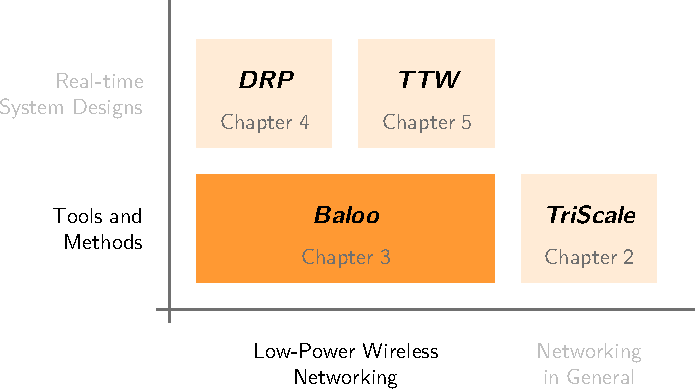
\includegraphics[scale=0.9]{chapter_baloo}
  \caption{Positioning of this chapter in the dissertation.
  \capt{This chapter presents \baloo, a design framework facilitating the implementation of low-power wireless networking protocols based on synchronous transmissions.}}
  \label{fig:chapter_baloo}
\end{figure}

% ------------------------------------------------------------------------------
% Claim
Thus, in this chapter, we study the feasibility of a design tool that would facilitate the development of network stacks based on \ST~(\cref{fig:chapter_baloo}); typically, such a tool would be useful for implementing our real-time protocol stacks (see \cref{ch:drp} and \cref{ch:ttw}).

\fakepar{Claim}
We propose and implement \baloo, a design framework for network stacks based on synchronous transmissions.
\baloo significantly lowers the entry barrier for harnessing the efficiency, reliability and mobility support of synchronous transmissions: users implement their protocol through a simple yet flexible API while \baloo handles all the complex low-level operations based on the users' inputs.

\baloo is flexible enough to implement a wide variety of network layer protocols, with only limited memory and energy overhead.

% ------------------------------------------------------------------------------
% Corresponding reference(s)
\begin{publi}

  The material from this chapter builds upon the work from Jonas Bächli~\cite{bachli2018Creating}. It relates to the following publication.

  \inlineRef{Synchronous Transmissions Made Easy: Design Your Network Stack with Baloo}{Romain Jacob, Jonas Bächli, Reto Da Forno, Lothar Thiele}{EWSN 2019. Beijung, China (February 2019)}

\end{publi}

% ------------------------------------------------------------------------------
% ------------------------------------------------------------------------------
% FORMER INTRO
% ------------------------------------------------------------------------------
% ------------------------------------------------------------------------------
% \newpage
% %Context
% \textsl{Synchronous Transmissions} (\ST) refers to a wireless communication technique that broadcast messages in a multi-hop network using flooding.
% This is made efficient by letting multiple transmitters send the \textsl{same packet} at the \textsl{same time}; henceforth the name of \emph{synchronous} transmissions.%
% \footnote{The name \textsl{concurrent transmissions} is also found in the literature.}
% \ST has been proven to be highly reliable and energy efficient, in particular for low-power wireless networks. Furthermore, flooding allows \ST to seamlessly support mobility by design.
% More informantion about \ST are presented in Introduction (\cref{ch:introduction}).
%
% %Problem
% Unfortunately, it is difficult to guarantee that multiple nodes actually send at the ``same time''.
% The required precision on synchronization depends \eg on the physical layer speed, the radio modulation speed or the encoding scheme.
% For typical low-power wireless motes available today, the synchronization must be in the order of \us for \ST to work reliably.
% Achieving such time synchronization requires to precisely control the timing of radio operations, which involves careful timer settings and interrupt handling.
% The integration of such ``low-level software'' within a entire network stack is challenging.
% Consequently, the adoption and development of \ST-based network stacks has been hindered by
% the lack of usable and flexible design tools.
%
% %Task and object
% Therefore, we developed \baloo: a flexible network stack design framework, designed to facilitate the development of protocols based on \ST. The key element of \baloo is a middleware layer which separates the radio management from the protocol implementation: \baloo provides a flexible application programming interface, while ensuring the correct timing of radio operations.
%
% %Findings
% \baloo is flexible enough to implement a wide variety of network layer protocols, with only limited memory and energy overhead.
% Most importantly \baloo makes \ST accessible: The software is open source and well documented.
% Since its development, \baloo has been used in a variety of projects, from both our team and external research groups.
% We believe that \baloo is an important enabler for a whole new class of Internet of Things applications leveraging the reliability, efficiency, and flexibility of \ST.

%
%
% This chapter presents \baloo, its design and the evaluation of its performance. We conclude with a brief description of projects that have been facilitated by \baloo, and finally discuss potential future developments, including standardization efforts.

% !TEX root =  ../00_thesis.tex

\section{Prolem Setting}
\label{sec:baloo_intro}

\squarepar{%
  Synchronous Transmissions (\ST) is an increasingly used wireless communication technology for low-power multi-hop networks. Popularized by Glossy~\cite{ferrari2011Glossy} in 2011, it has been proven to be highly reliable and energy efficient, as illustrated by the EWSN Dependability Competition ~\cite{schuss2017Competition}, where all wining solutions were based on \ST~\cite{escobar2018Competition,sommer2016Competition,lim2017Competition, escobar2019RedNodeBus, ma2019DeCoT} in the past four years (2016 to 2019).%
}

A \textsl{\ST primitive} refers to a protocol that efficiently realizes broadcast (\ie any-to-all communication) in bounded time, usually relying on \textsl{flooding}.
Flooding is a communication strategy that realizes broadcast by having all receivers of a packet retransmit this same packet to all their neighbours; the packet is thus ``flooded'' through the whole network. \ST makes flooding energy and time efficient by letting multiple wireless nodes transmit the packet \textsl{synchronously}, hence the name of \textsl{Synchronous Transmissions}. The successful reception of the packet can be achieved if the transmitters are tightly synchronized, thanks to \textsl{constructive interference} and the \textsl{capture effect}~\cite{yuan2013LetTalkTogether}.
The synchronization requirements vary from sub-\us to tens of \us, depending on the platform and modulation scheme~\cite{yuan2013LetTalkTogether}.
 %
%\footnote{Some background on flooding and \ST technology is provided in \cref{sec:baloo_overview}.}.
Such a broadcast primitive simplifies the design of network layer protocols: The underlying multi-hop network can be abstracted as a \textsl{virtual single-hop network} and thus be scheduled like a shared bus~\cite{ferrari2012LWB}.
One may refer to \cref{ch:introduction} for more details on \ST.

Since Glossy~\cite{ferrari2011Glossy}, many flavours of \ST primitives have been proposed to improve performance in terms of reliability, latency, and energy consumption.
To be more resilient to strong interference, Robust Flooding~\cite{lim2017Competition} is a primitive that modifies the RX-TX sequence from the original Glossy, whereas RedFixHop~\cite{escobar2016RedFixHop} uses hardware acknowledgements to minimize the number of retransmissions required.
Instead, some primitives aim to minimize latency for specific traffic patterns.
For example, Chaos~\cite{landsiedel2013Chaos} lets all nodes modify the packet being flooded to quickly aggregate information (\eg the max value of all sensor readings) or efficiently perform all-to-all data sharing to achieve distributed consensus~\cite{alnahas2017a2}.
Codecast~\cite{mohammad2018Codecast} also targets many-to-many exchange for a larger amount of data.
Pando~\cite{du2015Pando} is another primitive focused on high throughput, which uses fountain code and packet pipelining for efficient data dissemination.
Syncast~\cite{mohammad2017Improving} aims to reduce the radio on time required to save energy, while Less is More (LiM)~\cite{zhang2017LiM} is a primitive that reduces energy consumption using learning to avoid unnecessary retransmissions during flooding.

\squarepar{%
  All these primitives share the same drawback: Successful \ST requires low-level control of timers and radio events in order to meet \ST tight synchronization requirements (the order of \us).
  This degree of accuracy is difficult to achieve as it requires a detailed knowledge of the underlying hardware, low-level control of the radio operations, and a very careful management of software delays.%
}

As a result, designing a network stack based on \ST is a complex and time consuming task, for which only few solutions have been proposed.
One of the first was the Low-power Wireless Bus (LWB) ~\cite{ferrari2012LWB}, which tries to flexibly support all kinds of traffic patterns in a balanced trade-off between latency and energy consumption.
The same group designed eLWB~\cite{sutton2017eLWB}, a variation of LWB tailored to event-based data collection.
Sleeping Beauty~\cite{sarkar2016Sleeping} was later proposed to minimize energy consumption for data collection scenarios with many redundant sensor nodes.
Time-Triggered-Wireless (TTW -- \cref{ch:ttw})~\cite{jacob2017TTW_extended} was designed to minimize the end-to-end latency between communicating application tasks.
Finally, Crystal~\cite{istomin2018Interferenceresilient} has been proposed as a network stack specialized for sporadic data collection.
All these network stacks solely rely on Glossy as \ST primitive.
%
In principle however, the same protocol logic could benefit from \textsl{multiple} primitives. For example, an LWB network could use Robust Flooding~\cite{lim2017Competition} in case of high interference, then revert to Glossy~\cite{ferrari2011Glossy} for better time synchronization. If nodes need reprogramming, the software update can be quickly disseminated using Pando~\cite{du2015Pando}.
Designing a modular network stack supporting multiple \ST primitives adds a new level of complexity.

\begin{research_questions}
  \begin{description}
    \item[Question 1]
    Can we facilitate the design of wireless network stacks based on Synchronous Transmission?

    \item[Question 2]
    Can we implement flexible and adaptive protocols, potentially leveraging multiple \ST primitives, while guaranteeing that the timing requirements of \ST are met?
  \end{description}
\end{research_questions}

\fakepar{The problem}
To facilitate the network stack design (\question{1}),
a natural idea is to separate the concern of the timely execution of the primitives from the implementation of the protocol logic.
One way to achieve such separation of concerns is to use a \textsl{middleware} as part of the network stack.

%Challenges
The idea of a middleware for Wireless Sensor Networks (WSN) is not new, and the main challenge in such an endeavour is well-known.
As phrased by Mottola and Picco~\cite{mottola2012Middleware}, ``\textit{striking a balance between flexibility and complexity in providing access to low-level features is probably one of the toughest, yet most important, problems in WSN middleware}''.

The design of a middleware for \ST is particularly challenging.
Indeed, meeting the tight timing requirements for \ST is directly conflicting with the concept of abstraction of a middleware: How to guarantee that the network layer does not hinder the timing accuracy for \ST if it is itself unaware of the execution of the primitives? That is \question{2}.


\fakepar{The challenge} A middleware for \ST should meet the following requirements.
% This problem can be formulated by the following challenges:

\begin{features}

	\item[Usability]
	The middleware must realize a well-defined interface enabling runtime control from the network layer (which implements the protocol logic) over the execution of the underlying \ST primitives.

	\item[Generality]
	The middleware must enable the implementation of a large variety of network layer protocols.

	\item[Versatility]
	The middleware must enable one network layer protocol to use multiple \ST primitives and switch between them at runtime.

	\item[Synchronicity]
	The middleware must guarantee to respect the time synchronization requirements for \ST (from sub-\us to tens of \us~\cite{yuan2013LetTalkTogether}).
\end{features}

\pagebreak
%Task/Contibution
\fakepar{Our solution}
To address these challenges, we have designed \baloo, a flexible design framework for low-power network stacks based on \ST.%
\footnote{The framework provides the ``bare necessities'' for the design and implementation of \ST-based network stacks; so we called it \baloo.}
\baloo provides a large set of features enabling performant protocol designs, while abstracting away low-level hardware management such as interrupt handling and radio core control.
In summary:

\begin{itemize}
	\item
	We propose \baloo, a flexible design framework for low-power wireless network stacks based on \ST, illustrated in \cref{fig:stack_baloo}.

	\item
	We present the design of a middleware layer that meets all our requirements. This middleware forms the core component of \baloo.

	\item
	We showcase the usability of \baloo by re-implementing three well-known network stacks using \ST: the Low-power Wireless Bus (LWB)~\cite{ferrari2012LWB}, Sleeping Beauty~\cite{sarkar2016Sleeping}, and Crystal~\cite{istomin2018Interferenceresilient}.

	\item
	We illustrate the portability of \baloo by providing implementations for two platforms -- the CC430 SoC~\cite{CC430F6137} and the old but still heavily used TelosB mote~\cite{TelosB}.

	\item
	We demonstrate that \baloo induces only limited performance overhead (memory usage, radio duty cycle) compared to the original implementations.

\end{itemize}


\begin{figure}
  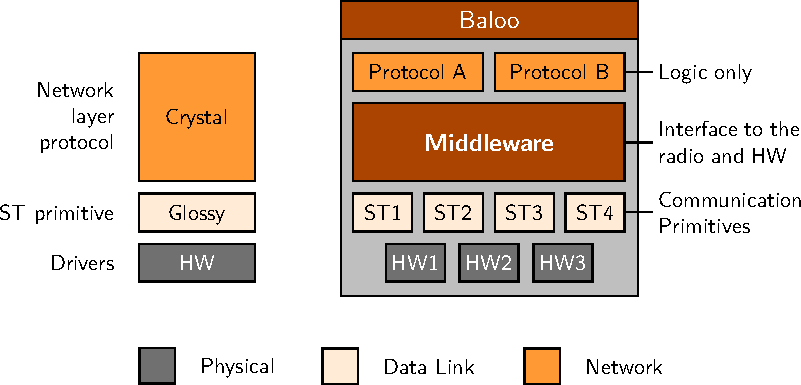
\includegraphics[scale=1]{stack_baloo.pdf}\\~\\
  \begin{minipage}[t]{.47\linewidth}
    \textbf{(a)} The implementation of the network layer protocol (Crystal) couples the interface to the underlying \ST primitive (Glossy) and the protocol logic, \ie how long are the communication rounds, which radio channel is used, \etc
  \end{minipage}
  \hfill
  \begin{minipage}[t]{.47\linewidth}
    \textbf{(b)} Thanks to its additional middleware layer, \baloo flexibly supports multiple \ST primitives and significantly reduces the efforts required to implement  network layer protocols compared to traditional stacks, like LWB~\cite{ferrari2012LWB} or Crystal~\cite{istomin2018Interferenceresilient}.
  \end{minipage}
  %
  \caption{Crystal~\cite{istomin2018Interferenceresilient} is a typical example of network stack based on \ST (\cref{fig:stack_baloo}a).
		Conversely, \baloo is a flexible design framework.
		It is based on a middleware layer that separates the concern of timely execution of \ST primitives from the implementation of the protocol logic (\cref{fig:stack_baloo}b).}
	\label{fig:stack_baloo}
\end{figure}

This chapter \emph{is not} meant to cover all details and inner mechanisms of \baloo, but mainly presents the core concepts of the framework.
\baloo is open source and the complete technical documentation is available online~(\cref{append:baloo_artifacts}).

% !TEX root = ../00_thesis.tex

\section{System Model}
\label{sec:problem}

Let \flowset be the set of real-time message \emph{flows} in the system.
The message release of each flow is \emph{sporadic with jitter}; \ie each flow $\flowi = (\flowsrci,\flowdsti,\periodi,\jitteri,\deadlinei)$ is defined by a \emph{source application} running on \emph{source node} \flowsrci that \emph{releases} messages with a \emph{minimum message interval} \periodi and \emph{jitter} \jitteri ($\jitteri < \periodi$), such that the time span of $n$ successive messages is never smaller than $(n-1)\times\periodi - \jitteri$ for any $n$. Every message released at $n_i^s$ should be delivered to the application running on \emph{destination node} \flowdsti within the  same \emph{relative end-to-end deadline}~$\deadlinei$.


The system model is illustrated in \cref{fig:DRP_sysmodel}: a set of \emph{nodes}~\nodeset exchange messages over a wireless multi-hop network; messages sent from a source node to a destination node are possibly relayed by multiple other nodes.
A logically global network manager, called the \emph{host}, arbitrates access to the network. Physically, the host may be one of the nodes.
The source and destination applications of a flow \flowi run on physically distributed nodes \flowsrci and \flowdsti.
Nodes can send to and receive messages from all other nodes in the system.

\begin{figure}
  \centering
  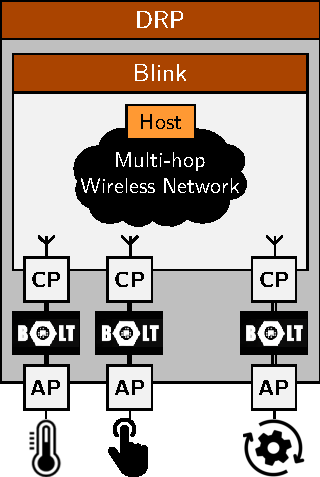
\includegraphics[scale=1]{stack_drp}
  \caption{System model of the \DRPLong (\DRP).
  \capt{A set~$\mathcal{N}$ of \DPP nodes are forming a wireless CPS.
  The communication processors (\CPs) run the \blink real-time protocol~\cite{zimmerling2017Blink} to exchange messages across a multi-hop wireless network.
  The \CPs forward and receive messages from their application processors (\APs) through \bolt~\cite{sutton2015Bolt}.
  \DRP is a global scheduler that arbitrates end-to-end communications between the \APs.
  On each \AP, the application tasks can be scheduled freely (\eg using a polling server, rate monotonic, \etc) as long as the resulting schedule satisfies the \DRP contracts~(\cref{sec:designDetailed}).
  The host is a (logically) global network manager which arbitrates the access to the shared wireless medium; \ie it runs the \blink and \DRP schedulers. Physically, one of the nodes plays the role of the host.}}
  \label{fig:DRP_sysmodel}
\end{figure}

\fakepar{Problem statement}
The problem is to design a wireless \CPS that fulfills all the requirements presented in \cref{sec:drp_intro} such that, for every message of every flow \flowi $\in \mathcal{F}$ released at the source node \flowsrci, if it is successfully transmitted by the wireless network, then it is delivered to the destination application running on node \flowdsti within the flow end-to-end deadline \deadlinei.

\squarepar{%}
  \fakepar{Application use case}
  Consider an acoustic wireless sensor network, such as those used to monitor permafrost in high alpine regions~\cite{weber2019decade,meyer2019IPSN}.
  Rock cracks are unpredictable events; however when one such event does happen, data must be collected and forwarded rapidly to a sink node for processing. For an early-warning system, it is crucial that this happens in real-time.
  Such an application perfectly matches our system model and motivates our problem statement.%
}

% !TEX root = ../00_thesis.tex

\section{Overview of \DRP}
\label{sec:design_overview}

\afterpage{
\begin{figure}
  \centering
  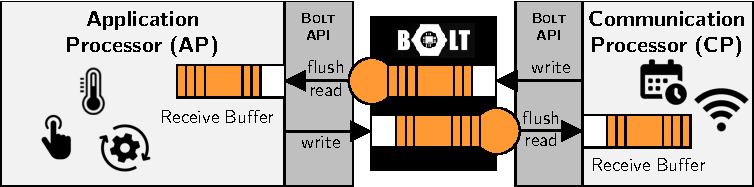
\includegraphics[scale=1]{dpp}
  \caption{Conceptual view of the DPP, based one the \bolt processor interconnect. %
  \capt{%
    Using functions \emph{\opwrite}, \emph{\opread}, and \emph{\opflush}, the application (\ap) and communication (\cp) processors can asynchronously exchange messages with predictable latency.
    The \AP executes application tasks (\eg sensing, actuation, control, \etc) while the \CP is dedicated to radio communication.}}
  \label{fig:bolt_logical}
\end{figure}
}

This chapter presents the \DRPLong (\DRP), a solution to provide end-to-end real-time guarantees between distributed applications.
Before delving into details, this section provides an overview of \DRP's principles.

The system model of \DRP divides the end-to-end communication between local and wireless parts~(\cref{fig:DRP_sysmodel}):
\begin{description}
  \item[\AP  $\boldsymbol{\leftrightarrow}$ \CP]
  Applications run on dedicated application processors (\APs) which are isolated from the rest of the network by their attached communication processor (\CP).
  Local communication between \APs and \CPs  takes place over the \bolt interconnect~\cite{sutton2015Bolt}, which provides asynchronous message passing with bounded delays.
  This device architecture, called the Dual-Processor Platform (\DPP), is illustrated in \cref{fig:bolt_logical} (more details in \cref{ch:introduction}).

  \item[\CP  $\boldsymbol{\leftrightarrow}$ \CP]
  The \CPs exchange messages over a multi-hop wireless network using the \blink real-time protocol~\cite{zimmerling2017Blink}.
  \blink is adaptive to dynamic changes in traffic demands, energy efficient, and delivers messages in real-time.
\end{description}

The \DPP and \blink are key building blocks to fulfill the \feature{Reliability}, \feature{Adaptability}, \feature{Composability}, and \feature{Efficiency} requirements.
However, two major issues remain in order to achieve \feature{Timeliness}.

First, the communication between \APs and \CPs cannot be completely asynchronous: to guarantee end-to-end deadlines, both processors must look for incoming messages with some minimal rate.
%
Second, \blink assumes a periodic release of messages at the network interfaces (\ie the \CPs); since our flow model is not periodic but sporadic with jitter~(\cref{sec:problem}), messages may be delayed in \CPs buffer until they can be transmitted over the network.

\DRP strikes a balance between  \feature{Composability} and \feature{Efficiency}; that is, between
\linebreak
\inlineitem decoupling the execution of \APs, \CPs, and Blink, \\
\inlineitem supporting short the end-to-end deadlines between the \APs.\\
The idea behind \DRP is to split the responsibility of meeting end-to-end deadlines between (i)~the source node $n^s_i$ and \blink, and (ii)~the destination node $n^d_i$;
If the source does not write too many messages, \blink guarantees every message will meet a given network deadline $D$, in turns, the destination commits to read its \bolt queue sufficiently often to meet the flow's end-to-end deadlines \deadlineany.

\DRP formalizes these ``commitments'' into \emph{contracts} between the different entities. The challenge is to define, given the current network state and an end-to-end deadline \deadlineany to satisfy, what must be
% \begin{itemize}
  % \item
  (i)~the network deadline $D$ requested to \blink and
  % \item
  (ii)~the minimal reading rate at the destination node.
% \end{itemize}
The goal is to make these contracts minimally restrictive, such that \APs, \CPs, and Blink can operate as much as possible independently from each other (\feature{Composability}).

% !TEX root = ../00_thesis.tex
%-------------------------------------------------------------------------------
\section{Designing \DRP}
\label{sec:designDetailed}
%-------------------------------------------------------------------------------

We now detail the three building blocks of our solution:
We first describe how \APs and \CPs exchange messages through \bolt~(\cref{subsec:boltAPI}), then we outline the operation of the \blink wireless real-time protocol~(\cref{subsec:details_blink}), and finally we present the detailed design of \DRP~(\cref{subsec:drp}).

%-------------------------------------------------------------------------------
\subsection{Bolt Processor Interconnect}
\label{subsec:boltAPI}

\bolt~\cite{sutton2015Bolt} provides predictable asynchronous message passing between two arbitrary processors, and hence decouples the processors with respect to time, power, and clock domains.
Concrete realizations of Dual-Processor Platforms (\DPP) based on \bolt are depicted in~\cref{append:dpp}.

\cref{fig:bolt_logical} shows a conceptual view of the DPP two message queues with first-in-first-out (FIFO) semantics, one for each direction, form the core of \bolt.
\bolt allows for concurrent \texttt{read} and \texttt{write} operations by \ap and \cp on both queues.

\bolt API includes three functions~(\cref{table:boltAPI}).
The \opwrite function appends a message to the end of the outgoing queue, whereas \opread reads and removes the first message from the incoming queue.
Calling \opflush results in a sequence of \opread operations until the incoming message queue is empty.
The implementation of \opflush is peculiar.
As \bolt allows for concurrent \opread and \opwrite operations, in theory, a \opflush may result in an infinite sequence of {\opread} operations.
To prevent this, the number of {\opread} during a \opflush is upper-bounded by $f_{max}$.
$f_{max}$ is set to the number of messages that fit into one \bolt queue, denoted by $S_{\bolt}$,
\begin{equation}
\label{eq:f_max=M}
f_{max} = S_{\bolt}
\end{equation}
Thus, a \opflush terminates when the incoming queue is found empty or when $f_{max}$ messages have been read out.

By design, \bolt API features predictable execution times, independently of the interconnected processors~\cite{sutton2015Bolt}.
We denote by $C_w$, $C_r$, and $C_f$ the worst-case execution times~(WCETs) of \opwrite, \opread, and \opflush.

\begin{table}
\centering
\caption{\bolt application programming interface (API)}
  {\smaller
  \begin{tabularx}{\linewidth}{@{}c@{\qquad}X@{\qquad}c@{}}
    \toprule
      \textbf{Function} & \multicolumn{1}{c}{\textbf{Description}} & \textbf{WCET} \\
    \midrule
      \texttt{write}
    	& Append a message to outgoing queue
    	& $C_w$ \\[10pt]
      \texttt{read}
      & Read and remove the first message from incoming queue
      & $C_r$ \\[10pt]
      \texttt{flush}
      & Perform up to $f_{max}$ \texttt{read} operations, or until incoming queue is empty
      & $C_f = f_{max}*C_r$\\
    \bottomrule
  \end{tabularx}}
\label{table:boltAPI}
\end{table}

\subsection{Blink Wireless Real-time Protocol}
\label{subsec:details_blink}

\afterpage{
\begin{figure}
 \centering
 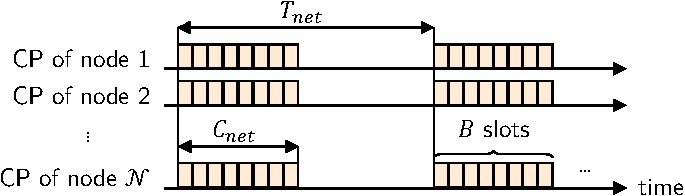
\includegraphics[scale=1]{blink_overview}

 \caption{Operations in \blink are globally time-triggered. \capt{Communication occurs in rounds of equal duration \rlength. Each round consists of a sequence of up to \nslotsmax exclusive time slots, each of which serves to send one message using Glossy floods~\cite{ferrari2011Glossy}.
 The time interval between two consecutive rounds (\rperiod) may vary.
 During a round, the \CP of all nodes in the system participate in the flood.}}

 \label{fig:blink_overview}
\end{figure}
}

In \blink~\cite{zimmerling2017Blink}, wireless multi-hop communication is globally time-triggered and occurs in {rounds} of equal {duration} \rlength~(\cref{fig:blink_overview}).
Each round serves to send up to \nslotsmax messages within exclusive time slots.
In each time slot a message is sent from a given \cp to all other \CPs using Glossy floods, which deliver packets with a probability above 99.9\,\%~\cite{ferrari2011Glossy}.%
%
\footnote{The principle of round-based communication using Glossy floods was introduced in the Low-power Wireless Bus (LWB)~\cite{ferrari2012LWB}. The concept was later adapted in many different flavors~(see the introduction of \cref{ch:baloo}).
\blink is a real-time scheduler for LWB.}
%
The interval between the start of consecutive rounds, denoted by \rperiod, is determined by the host at runtime based on current real-time traffic demands. \rperiodmin and \rperiodmax are implementation-specific bounds on \rperiod.
\blink defines \rperiod and the assignment of messages to rounds such that the number of rounds is minimized and all messages meet their \emph{network deadline} \ndeadlinei between network interfaces (\ie the \CPs).

\blink communication rounds are atomic: during a round, all \CPs are busy executing \blink; other tasks (\eg exchanging messages through \bolt) can only be executed between rounds.
Furthermore, \blink assumes constrained deadlines ($\ndeadlinei \leq \periodi$).
Thus, the network deadline \ndeadlineany must be larger than the minimal round interval and smaller than the flow period \periodany
\begin{equation}
  \rperiodmin \leq \rperiod \leq \ndeadlineany \leq \periodany
\end{equation}

\blink expects periodic message arrivals with a known initial phase for the first packet.
We refer to this as the expected arrival pattern.
For any message matching the expected arrival pattern,
\blink guarantees that, if the message is successfully received at the destination \cp, the message meets its relative network deadline~\ndeadlineany.%

However, we must consider the complete system:
(i)~the message release from the \APs is sporadic with jitter, and
(ii)~\APs and \CPs operate independently~(\feature{Composability}). Thus, there is a mismatch between the periodic arrival pattern assumed by \blink and the actual message arrival at the \CPs.

\subsection{\DRP: Distributed Real-time Protocol}
\label{subsec:drp}

\blink provides real-time guarantees between the network interfaces (\ie the \CPs) assuming periodic message release. \DRP handles the mismatch between the \blink assumptions and the actual message arrival at the \CPs by
(i)~letting the host \emph{assume} that messages are indeed released periodically at the \CPs.
  \blink's communication schedule is computed based on the expected arrival pattern and using an arbitrary initial phase for the flows.
(ii)~analyzing the maximal mismatch between the actual and expected arrival patterns.

This upper-bound represents the maximum extra-delay that a message can suffer before it is scheduled for communication by \blink.
Then, the delay bounds for communication over \bolt and over the wireless network can be combined into a worst-case latency analysis which connects the system parameters (such as the network deadlines and flushing rate of \bolt) with the expected message latency.
\DRP reverts these relations to define values for the system parameters
that guarantee to meet the specified end-to-end deadlines.
\DRP enforces such parameter values using contracts, which are agreed upon at runtime every time a new message flow is registered.

\fakepar{Contracts}
\DRP contracts are key to fulfill the \feature{Timeliness} and \feature{Reliability} requirements. Concretely, these contracts
\begin{itemize}
  \item avoid overflows of message buffers (\eg the \bolt queues) at the source and destination nodes, thus preventing message losses;
  \item ensure that messages are handled ``fast enough'' between the network (\ie \CPs) and the application (\ie \APs) interfaces by the source and destination nodes, such that all messages meet their end-to-end deadlines.
\end{itemize}

To avoid overflows, \DRP defines {maximum time intervals} between two \opflush operations of \bolt by the \CPs and \APs, denoted by $T_f^s$ and $T_f^d$ respectively.
$T_f^s$ is statically set for all \CPs in order not to constrain the achievable end-to-end deadline.
Conversely, $T_f^d$ is adjusted dynamically by the destination nodes upon registration of a new flow.

Providing end-to-end guarantees entails that \DRP decides on the {distribution of responsibilities} among the source node, \blink, and the destination node of a flow \flowi with regard to meeting the end-to-end deadline \deadlinei. To this end, \DRP uses the \emph{deadline ratio}~$r \in (0,1)$, a global parameter chosen at design time.
The joint responsibility of the source and \blink is a function of the source flushing interval $T_f^s$ and the flow's network deadline \ndeadlinei~(computed by \DRP -- \cref{fig:design_overview}). They are responsible for meeting a fraction $r$ of the end-to-end deadline
\begin{equation}\label{eq:function_f}
 f(T_f^s,\ndeadlinei) \; \leq \; r * \deadlinei
\end{equation}
The remaining part of the end-to-end deadline defines the responsibility of the destination, which is a function of its flushing interval $T_f^d$
\begin{equation}\label{eq:function_g}
 g(T_f^d) \; \leq \;  (1-r) * \deadlinei
\end{equation}
In \cref{sec:concrete_realization}, we derive concrete expressions for the functions $f$ and $g$, and we specify how \DRP computes \ndeadlinei and $T_f^d$.
In \cref{sec:drp_evaluation} we illustrate how the choice of the deadline ratio $r$ influences the achievable bandwidth and end-to-end guarantees of our wireless \CPs system.

For each newly admitted flow $\flowi = (\flowsrci,\flowdsti,\periodi,\jitteri,\deadlinei) \in \flowset$, \DRP dynamically establishes two contracts.

\begin{itemize}
	\item \textbf{Source} $\boldsymbol{\leftrightarrow}$ \textbf{Blink}
  \quad
  \flowi's source application, which runs on \apsrc at node  \flowsrci, agrees to write no more messages than specified by the minimum message interval \periodi and the jitter \jitteri. The attached \cpsrc prevents overflows of \bolt and its local message buffer.
	In turn, \blink agrees to serve flow \flowi such that any message matching the expected arrival of \flowi meets its network deadline \ndeadlinei.

	\item \textbf{Blink} $\boldsymbol{\leftrightarrow}$ \textbf{Destination}
  \quad
  \blink agrees to deliver no more messages than specified by \periodi.
	In turn, \cpdst and \apdst agree to read out all delivered messages such that overflows of \bolt and \cpdst's local  buffer are prevented and all messages meet \flowi's end-to-end deadline~\deadlinei.
\end{itemize}

For any flow, if both contracts are fulfilled, all messages that are successfully delivered by \blink will meet their end-to-end deadline. In practice, the contracts fulfillment is guaranteed by a set of \emph{admission tests}, which are performed in sequence upon registration of a new flow, as described next.

\afterpage{
\begin{landscape}
  \begin{figure*}
  \centering
  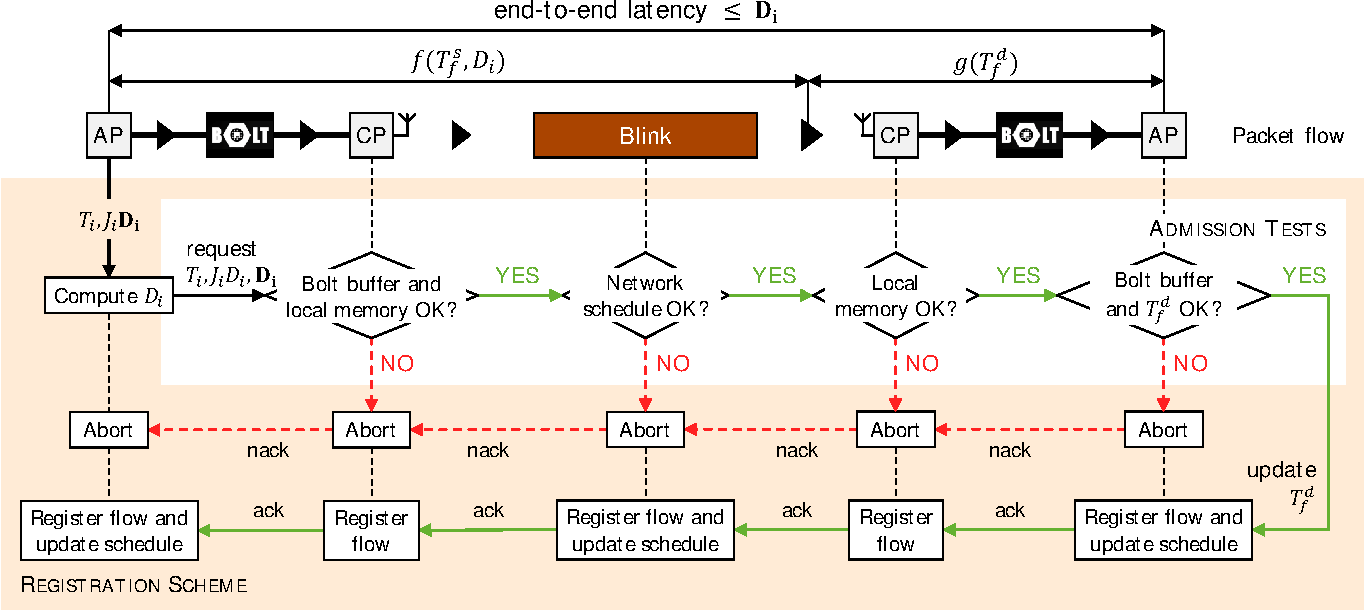
\includegraphics[scale=1]{registration_scheme}

  \caption{Steps and components involved when registering a new flow in \DRP. \capt{Given a request for a new flow $\flowi = (\flowsrci,\flowdsti,\periodi,\jitteri,\deadlinei)$, the source application running on \apsrc at node \flowsrci computes the flow's network deadline \ndeadlinei. Then, all components check one after the other using specific admission tests whether they can admit the new flow. \DRP registers a new flow only if all admission tests succeed, which eventually triggers changes in the runtime operation (the schedule) of \blink as well as of the source and destination application processors \apsrc and \apdst.}}

  \label{fig:design_overview}
  \end{figure*}
\end{landscape}
}

\fakepar{Flow registration}
\cref{fig:design_overview} shows the full procedure for registering a new flow $\flowi = (\flowsrci,\flowdsti,\periodi,\jitteri,\deadlinei)$ in \DRP.
The flow's source application running on \apsrc first computes the network deadline \ndeadlinei (\cref{sec:concrete_realization}) before it writes the request to the attached \cpsrc through \bolt.
\cpsrc uses its admission test to check whether it could still prevent overflows of \bolt and its local memory if \flowi were present.
If so, \cpsrc forwards the request to the host, which checks the schedulability using \blink's admission test~\cite{zimmerling2017Blink}.
If \blink admits the flow, the destination node's \cpdst and \apdst check whether they can prevent overflows of \cpdst's local memory and \bolt, respectively.
Moreover, \apdst re-computes its required flushing interval $T_f^d$ and checks using mainstream schedulability analysis~\cite{buttazzo2011HardRT} whether it can support this new load (in addition to the load incurred by other tasks running on \apdst).
\DRP registers a flow only if all admission tests succeed, which then triggers changes in the runtime operation of \apsrc, \blink, and \apdst.

Flow requests and acknowledgments are sent via dedicated control flows, which are registered by default at bootstrapping for each node in the network.

\afterpage{
\begin{figure}
 \centering
 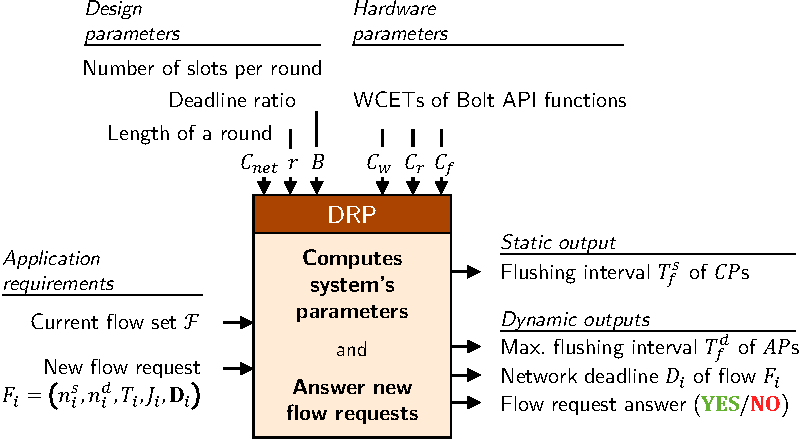
\includegraphics[scale=1]{inputs_outputs}
 \caption{Inputs and outputs of \DRP.
  \capt{Hardware and design parameters are fixed at design time, while the application requirements may change at runtime. \DRP statically computes the flushing interval of \CPs; all other outputs are dynamically computed whenever the flow set $\mathcal{F}$ changes.}}
 \label{fig:procedure_overview}
\end{figure}
}


\fakepar{\DRP procedure}
\cref{fig:procedure_overview} summarizes all the inputs and outputs of \DRP.
Hardware parameters (related to \bolt) and design parameters (\ie the length of a communication round \rlength, the deadline ratio $r$, and the number of slots per round \nslotsmax) are constants known at compile time.
The application's real-time communication requirements may change at runtime as new flows are requested and existing flows are removed. \DRP determines $T_f^s$ statically, while all other outputs are dynamically computed whenever the set of flows changes, according to the procedure illustrated in \cref{fig:design_overview}.

% !TEX root = ../00_thesis.tex

\section{Concrete Realization of \DRP}
\label{sec:concrete_realization}

This section discusses how to concretely implement \DRP's concepts. In particular, one needs to define
% \begin{itemize}
  % \item
(i)~the fixed flushing interval $T_f^s$ of the \CPs~(\cref{subsec:CP_schedule}), and
  % \item
(ii)~how to dynamically compute the network deadline \ndeadlinei of a flow \flowi and the flushing interval $T_f^d$ of each \ap (\cref{subsec:D_Tfd_computation}).
% \end{itemize}

Then, a worst-case buffer analysis (\cref{subsec:WC_buffer}) will allow to formulate admission tests (\cref{subsec:admission}), one for {\ap}s and one for {\cp}s.
The success of all admission tests guarantees that both contracts \textbf{Source}~$\boldsymbol{\leftrightarrow}$~\textbf{Blink} and \textbf{Blink}~$\boldsymbol{\leftrightarrow}$~\textbf{Destination} can be satisfied by \DRP.

\subsection{Setting \CPs' Flushing Interval}\label{subsec:CP_schedule}

To guarantee that all \CPs fulfill their share of the contracts (\ie prevent buffer overflows), we conceive a time-triggered approach to schedule all tasks of \CPs. It consists of (\emph{i}) setting the flushing interval $T_f^s$ of all \CPs to the same constant value, and (\emph{ii}) letting the round interval $T_{net}$ be a multiple of $T_f^s$.
As discussed in \cref{sec:designDetailed}, $T_f^s$ should not to constrain the achievable deadline: thus, we aim to set it as short as possible.
\CPs have three tasks to perform
\begin{itemize}
 \item flushing \bolt before each communication round,
 \item participating in the communication during the rounds,
 \item writing all received messages into \bolt after the rounds.
\end{itemize}
Performing those tasks altogether takes $C_{CP} + C_{net}$ time units, where $C_{CP} = C_f + \nslotsmax * C_w$, and \nslotsmax denotes the number of time slots in one round.
Hence, $C_{CP} + C_{net}$ is the smallest admissible round interval (otherwise \CPs' task set is not schedulable). Thus we set for all \CPs in the system,
\begin{align}
\label{eq:design_flush_period_source}
	& T_f^s = C_{CP} + C_{net} \\
\intertext{and we let the round interval be a multiple of $T_f^s$. In other words, for $k \in \mathbb{N}$, $k > 0$,}
\label{eq:design_round_period}
	& T_{net} = k * T_f^s
\end{align}
For a given $C_{net}$, a larger $k$ entails less available bandwidth but also lower energy consumption.
\blink is designed to dynamically adjust $k$ to match the bandwidth requirements and save energy~\cite{zimmerling2017Blink}.

\subsection{\mbox{Computing Network Deadlines \& \APs ' Flushing Interval}}
\label{subsec:D_Tfd_computation}

Having fixed \CPs' flushing interval, we now turn to the problem of dynamically computing the network deadline \ndeadlinei of flow \flowi and the flushing interval $T_f^d$ of \flowi's destination \apdst, such that the end-to-end deadline \deadlinei is met.
To this end, we need to define expressions for the functions $f$ and $g$ (introduced in \cref{sec:designDetailed}), and derive values for \ndeadlinei and $T_f^d$ such that equations \eqref{eq:function_f} and \eqref{eq:function_g} are satisfied.

\begin{theorem}
  \label{thm:delta}
  For any flow \flowi = (\flowsrci,\flowdsti,\periodi,\jitteri,\deadlinei), and given the duration of communication rounds $C_{net}$, functions $f$ and $g$ are upper-bounded as follows
  \begin{align}
  f(T_f^s ,  \ndeadlinei)
  	& \; \leq \;
  	T_i + D_i + \overline{\jitteri}  + \delta_f^{const} \label{eq:expression_f}\\
  g(T_f^d)
  	& \; \leq  \;
  	T_f^d(\flowdsti) + \delta_g^{const} \label{eq:expression_g}
  \end{align}
  where $ \delta_f^{const}$ and $\delta_f^{const}$ are constant delays that depend on the WCETs of the \bolt API functions, on the maximum number of messages \nslotsmax that can be %inside a \bolt queue at the end of a round
  served by \blink in one round, and on the fixed flushing interval $T_f^s$ of \CPs,
  \begin{align}
  \delta_f^{const} &\;= \;\; C_w + C_f + T_f^s \\
  \delta_g^{const} &\;= \;\;\nslotsmax*C_w - (\nslotsmax-1)* C_r + C_f\\
  \label{eq:jitter_bar}
  \overline{\jitteri}  &\;= \;\; \floor*{(\jitteri + C_f - C_r)/{T_f^s}}\cdot T_f^s
  \end{align}
\end{theorem}

\begin{proof}%
Function $f$ is the time between when a message is written into \bolt by the source \apsrc and when the communication round in which the message is sent by \blink ends (\ie when the message is available at the destination \cpdst).
This is the sum of two delays: $\delta_{source}$, the time until the message is available for communication at the source \cpsrc; and $\delta_{network}$, the time until the message is shipped over the network to \cpdst.

Similarly, function $g$ is the time between when a packet is available at the destination \cpdst and the end of the \opflush operation that reads the message out of \bolt at the destination \apdst (\ie when the message can be processed by the destination application).
We refer to this delay as $\delta_{dest}$.

Hence, the expressions for functions $f$ and $g$ in \eqref{eq:expression_f} and \eqref{eq:expression_g} directly follow from the delays expression derived in Lemmas~\ref{lem:delta_source}, \ref{lem:delta_network}, and \ref{lem:delta_destination}~(\cref{append:drp_WCanalysis}).
\
\end{proof}

We use Theorem~\ref{thm:delta} to express conditions on \ndeadlinei and $T_f^d$ such that \eqref{eq:function_f} and \eqref{eq:function_g} are satisfied.
In particular, it is sufficient that for any flow $\flowi = (\flowsrci,\flowdsti,\periodi,\jitteri,\deadlinei) \in \flowset$
\begin{align}
\nonumber
 T_i + D_i + \overline{\jitteri} \;
	& \leq  \;\; r * \deadlinei - \delta_f^{const} \\
\label{eq:ndeadline_constraint_latency}
\Rightarrow \qquad T_i \;
	& \leq  \;\; r * \deadlinei - \delta_f^{const} - D_i - \overline{\jitteri} \\
\intertext{and}
\label{eq:APflush_constraint_base}
T_f^d(\flowdsti) \;
	& \leq \, (1-r)*\deadlinei -  \delta_g^{const}
\end{align}

As low-power wireless networks typically feature limited bandwidth,%
\footnote{Low-power radio bit rates are often limited to 256\kbps; the latest version of Bluetooth (Bluetooth~5) supports up to 2\Mbps.}
%
it makes sense to choose the network deadline \ndeadlinei as large as possible in order to increase the schedulability of flows in the network.
However, \blink only supports constrained deadlines ($\ndeadlineany \leq \periodany$) and deadlines must be multiples of the round length ($\ndeadlineany = 0 \mod \rperiod $).
Furthermore, a network deadline cannot be smaller than \rperiodmin (see \cref{subsec:details_blink}).
%
Hence, for any flow \flowi, it must hold that
\begin{align}
  \label{eq:ndeadline_constraint_period}
  \rperiodmin \; &\leq \; \ndeadlinei \; \leq \; \periodi \\
  \ndeadlinei \; &= \; 0 \mod \rperiod
\end{align}

Finally, to satisfy all contracts in the system, \eqref{eq:ndeadline_constraint_latency}, \eqref{eq:APflush_constraint_base} and \eqref{eq:ndeadline_constraint_period} must hold for all flows $\flowi \in \flowset$.
Hence, the values for \ndeadlinei and $T_f^d$ computed dynamically at runtime must satisfy for any flow $\flowi = (\flowsrci,\flowdsti,\periodi,\jitteri,\deadlinei) \in \flowset$ and any $n \in \mathcal{N}$
\begin{align}
\label{eq:design_ndeadline}
\ndeadlinei \;
	& = \; \min \left(\; \periodi \;\, , \,  r*\deadlinei - \delta_f^{const} - \periodi - \overline{\jitteri} \right) - (\ndeadlinei \mod \rperiod) \\
\label{eq:design_delay_destination}
T_f^d(n) \;
	& \leq \; \min_{F_j\in \mathcal{F}, n = \flowdstj}
	\left( (1-r)*\deadlinej - \delta_g^{const} \right)
\end{align}
If using \eqref{eq:design_ndeadline} leads to a violation of the constraint in \eqref{eq:ndeadline_constraint_period} or if $T_f^d$ results in a load that \ap at node $n$ cannot handle, \DRP rejects the flow since the two contracts cannot be guaranteed.


\subsection{Worst-case Buffer Analysis}
\label{subsec:WC_buffer}

Satisfying all contracts entails preventing overflows of message buffers in the system.
Specifically, as shown in \cref{fig:design_overview},
\begin{itemize}
	\item \APs are responsible for ensuring that the incoming \bolt queues do not overflow, and
	\item \CPs are responsible for ensuring that their local message buffers and the outgoing \bolt queues do not overflow.
\end{itemize}

To formulate the admission tests for {\ap}s and {\cp}s, we first need the worst-case buffer sizes (\ie maximum number of messages in a buffer) induced by a given flow set \flowset.
For ease of exposition, we make the following hypothesis.
\begin{hypothesis}\label{hyp:f_max}
For a given flow set \flowset, an \ap (resp. \cp) never writes more messages into \bolt than can be flushed by \cp (resp. \ap) in one \emph{\opflush} operation in the time span between two \emph{\opflush}.
\end{hypothesis}
This hypothesis implies that the \bolt queues are always empty at the end of a \opflush operation.
We prove at the end of this section that our admission tests effectively guarantee that Hypothesis~\ref{hyp:f_max} is always verified.

\begin{lemma} \label{lem:buffer_bolt_out}
Given a flow set \flowset, the buffer size of the outgoing \bolt queue of node $n \in \nodeset$, $B_{\bolt,out}(n)$, is upper-bounded,
\begin{equation}
\label{eq:bolt_out_buffer_stress}
	B_{\bolt, out}(n) \; \leq \;
	\sum_{\substack{F_i\in \mathcal{F},\, n = \flowsrci}} \ceil*{\frac{T_f^s + C_w + C_r + \jitteri}{T_i}}
\end{equation}
\end{lemma}

\begin{proof}%
According to the \textbf{Source} $\boldsymbol{\leftrightarrow}$ \textbf{Blink} contract, \apsrc at node $n$ does not write more than one message every \periodi with jitter \jitteri into the outgoing \bolt queue.
Based on Hypothesis~\ref{hyp:f_max}, the buffer size is bounded by the number of messages that can be written by \apsrc during the maximum time a message can stay inside the queue, which is $\Delta = T_f^s + C_w + C_r$ (see \cref{fig:delta_source_time_graph}).
The maximum number of messages that can be written by \apsrc within any time interval $\Delta$ is $\ceil*{(\Delta + J_i)/{T_i}}$ for each flow \flowi sourced by~$n$. \
\end{proof}


The worst-case buffer size of a \cp depends on (i) the maximum time a message can stay in \cp's local memory awaiting to be served by \blink, and (ii) the number of messages that can be sent within one round to a node.

\begin{lemma} \label{lem:buffer_CP}
Given a flow set \flowset, the buffer size of {\cp}'s internal memory of node $n \in \nodeset$, $B_{CP}(n)$, is upper-bounded,
\begin{equation}
\label{eq:CP_memory_stress}
	B_{CP}(n) \leq
	\sum_{\substack{F_i\in \mathcal{F},\\ n = \flowsrci}}
	1 + \ceil*{\frac{\ndeadlinei + \overline{\jitteri} + C_f}{T_i}} +
	\sum_{\substack{F_i\in \mathcal{F},\\ n = \flowdsti}} 1
\end{equation}
\end{lemma}

\begin{proof}%
On the source side, we make the conservative assumption that all messages read out during a \emph{\opflush} occupy memory in \cpsrc from the beginning of the \emph{\opflush}. Hence, the maximum waiting time in \cpsrc for a message until it is served by \blink is $\delta_{network} + C_f$ (see Lemma~\ref{lem:delta_network} -- \cref{append:drp_WCanalysis}). The number of messages in \cpsrc due to the source is upper-bounded by the maximum number of messages \apsrc can write during this time interval, given by
$\ceil*{\delta_{network} + C_f)/T_i}$.
Using Lemma~\ref{lem:delta_network}, this is at most
$1 + \ceil*{( \ndeadlinei + \overline{\jitteri} + C_f)/\periodi }$  per outgoing flow.



One the destination side, during a round, \cpdst may receive several messages, which it immediately writes into \bolt after the round.
However, \blink expects one packet every \periodi from each flow, which it serves within \ndeadlinei. As $\ndeadlinei \leq \periodi$, \blink never schedules more than one packet per round for each flow.
Thus, the maximum number of messages in \cpdst due to the destination is 1 packet per incoming flow.
\
\end{proof}

\begin{lemma} \label{lem:buffer_bolt_in}
Given a flow set \flowset, the buffer size of the incoming \bolt queue of node $n \in \nodeset$, $B_{\bolt,in}(n)$, is upper-bounded,
\begin{equation}
\label{eq:bolt_in_buffer_stress}
	B_{\bolt, in}(n)\;  \leq \;
	\sum_{\substack{F_i\in \mathcal{F},\\ n = \flowdsti}} \ceil*{\frac{T_f^d(n) + C_w + C_r + D_i}{T_i}}
\end{equation}
\end{lemma}

\begin{proof}%
As specified in the \textbf{Source} $\boldsymbol{\leftrightarrow}$ \textbf{Blink} contract, \blink delivers packets from any flow \flowi before the network deadline \ndeadlinei~(\cref{sec:designDetailed}). Therefore, \blink delivers at most one packet every \periodi time units, with a jitter equal to \ndeadlinei, which are written into \bolt immediately after the round.

Based on Hypothesis~\ref{hyp:f_max},
the buffer constraint of the incoming \bolt queue is bounded by the number of packets that can be written by \cpdst during the maximum elapsed time before a packet is read out by \apdst. As in the proof of Lemma~\ref{lem:buffer_bolt_out}, there are at most $\ceil*{(T_f^d(n) + C_w + C_r + D_i)/{T_i}}$ such messages from each flow \flowi that has node $n$ as destination.
\end{proof}


\subsection{Admission Tests}
\label{subsec:admission}

We now combine the above results and formulate the admission tests for \CPs and \APs, which form the cornerstone of \DRP's registration mechanism described in \cref{sec:designDetailed}.
We further show that the computation complexity of the admission tests is not only small but \emph{constant}, and hence supports the requirements of \feature{Adaptability} and \feature{Efficiency}.

Let $F_j$ be the flow for which a request has been issued, and $\mathcal{F}_{new} = \mathcal{F} \cup \{F_j\}$.
The \cp of node $n$ is responsible for preventing overflows of its local memory (of size $S_{CP}$) and of the outgoing \bolt queue of node $n$ (of size $S_{\bolt}$).

\begin{theorem}[{Admission Test of \cp}]\label{thm:CP}
If
\begin{align*}
S_{\bolt} \;
	 & \geq \sum_{\substack{\flowi \in \mathcal{F}_{new}, \\ n = \flowsrci}}
	 	\ceil*{\frac{T_f^s + C_w + C_r + \jitteri}{T_i}} \\
\textup{and}\qquad
S_{CP} \;
 	& \geq
	\sum_{\substack{\flowi \in \mathcal{F}_{new}, \\ n = \flowsrci}}
		1 + \ceil*{\frac{\ndeadlinei + \overline{\jitteri} + C_f}{T_i}}
	+ \sum_{\substack{\flowi \in \mathcal{F}_{new}, \\ n = \flowdsti}}
		1
\end{align*}
then the requested flow \flowj can be safely admitted by $\cp$.
\end{theorem}

\begin{proof}Immediate from Lemmas~\ref{lem:buffer_bolt_out} and \ref{lem:buffer_CP}. \
\end{proof}


The \ap of node $n$ is responsible for preventing overflows of the incoming \bolt queue (of size $S_{\bolt}$) and for guaranteeing its share of the end-to-end deadline.

\begin{theorem}[{Admission Test of \ap}]
\label{thm:AP}
  If there exists $T_f^d(n)$ such that
  \begin{align*}
    T_f^d(n) \;
    & \leq \, \min_{\substack{F_i\in \mathcal{F}_{new}, \\  n = \flowdsti}}
    \left( (1-r)*\deadlinei - \delta_g^{const} \right)\\
\textup{and}\qquad
    S_{\bolt} \;
    & \geq \sum_{\substack{\flowi \in \mathcal{F}_{new}, \\ n = \flowdsti}} \ceil*{\frac{T_f^d(n) + C_w + C_r + D_i}{T_i}}
  \end{align*}
  then the requested flow \flowj can be safely admitted by $\ap$.
\end{theorem}
\begin{proof}
Immediate from Lemma~\ref{lem:buffer_bolt_in} and equation \eqref{eq:design_delay_destination}.
\end{proof}

Finally, we verify that Hypothesis~\ref{hyp:f_max} holds, showing the validity of our buffer analysis. From \eqref{eq:f_max=M} we have $f_{max} = S_{\bolt}$. Thus, by performing the admission tests at runtime, it follows from Theorems~\ref{thm:CP} and \ref{thm:AP} and Lemmas~\ref{lem:buffer_bolt_out} and \ref{lem:buffer_bolt_in} that $f_{max}$ is always bigger than the filling level of any \bolt queue, which entails Hypothesis~\ref{hyp:f_max} is true.

% !TEX root = ../00_thesis.tex

%-------------------------------------------------------------------------------
\section{Implementating \DRP}
\label{sec:drp_implementation}
%-------------------------------------------------------------------------------

This dissertation aims to provide concrete solutions for wireless \CPS, not only theoretical concepts. It is therefore important to implement the concepts and evaluate their performance when running on real hardware.
This section presents some important design choices we made for our implementation of \DRP.
%
The performance evaluation is presented in \cref{sec:drp_evaluation}.

%-------------------------------------------------------------------------------
% \subsection{Design Choices}



\DRP extends \blink~\cite{zimmerling2017Blink}, which is a real-time scheduler for LWB~\cite{ferrari2012LWB}. Thus, we start our implementation of \DRP from an existing implementation of LWB~\cite{Code_LWB}. There are two main functionality to implement for running \DRP
\begin{itemize}[nosep]
  \item
% (i)~
compute \blink schedules, and
  \item
% (ii)~
perform \DRP admission tests.
\end{itemize}

\DRP leverages the \DPP design by having all the computations performed by the \AP while the \CP only runs LWB.
From an implementation stand-point, the challenge is that the \AP does computations but the \CP needs the results (\eg the LWB schedules); the communication over \bolt between \AP and \CP  must happen in a way that does not interrupt or delay LWB operations.
Moreover, the memory and computational requirements of the protocol must be compatible with the (typically limited) capacity of embedded hardware.

\fakepar{Task distribution}
On all nodes, the computations related to \DRP admission tests are performed by the \AP, including \CP's buffer checks~(\cref{thm:CP}).
These tests only require minimal state keeping, which can be easily delegated to the \AP. This has two benefits: (i)~it limits the modification to the \CP firmware (\ie LWB) and (ii)~it improves performance (the admission test is more efficiently computed by the \AP than by the \CP).

\fakepar{Round structure}
Our implementation maintains the original LWB round structure, only removing the contention slot~(\cref{fig:drp_round}). This slot becomes redundant in \DRP since each node bootstraps with registered control flows, which are used for further \DRP requests and flow registrations~(\cref{sec:designDetailed}).

\begin{figure}
  \centering
  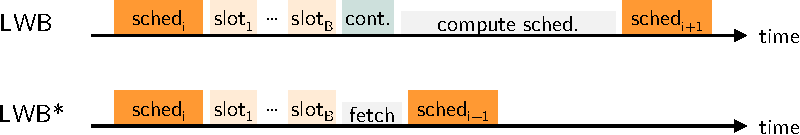
\includegraphics[scale=1]{drp_round}
  \caption{The original LWB (Top) and the modified round used in \DRP (Bottom).
  \capt{\DRP removes the contention slots, made redundant by the presence of dedicated control flows. Furthermore, the time span before sending the next round's schedule can be significantly reduced: indeed in \DRP, the host \CP can quickly fetch the schedule from the \AP, which has done the computation in parallel.}}
  \label{fig:drp_round}
\end{figure}

\fakepar{Schedule fetch}
The host \CP fetches the schedule for the LWB round $i+1$ at the end of round $i$~(\cref{fig:drp_round}).
\CP requests the schedule to \AP, which maintains the schedule ready and writes it to \bolt whenever the request comes.

\fakepar{Communication model}
The communication between \AP and \CP over \bolt can be based on polling or interrupts. When using polling, processors asynchronously check the status of their incoming \bolt queue to check whether a message is present. Conversely, an interrupt can be generated at the receiving processor whenever a \bolt \texttt{write} operation is completed.
\begin{description}

  % \item[\AP $\boldsymbol{\rightarrow}$ \CP]
  \item[\AP to \CP]
  When \AP writes to \bolt, we trigger an interrupt on the \CP and read out the message immediately.
  Since \DRP flow model is sporadic and new packets are expected infrequently~(\cref{sec:problem}), using interrupt is fast, energy efficient, and avoids building up the \bolt queue.

  However, during LWB rounds, it is paramount that \CP operations are not delayed or disturbed. Thus, during the rounds, interrupts are disabled and (potential) new messages written by \AP are read out after the round.

  % \item[\CP $\boldsymbol{\rightarrow}$ \AP]
  \item[\CP to \AP]
  We assume that the \AP on the host node is dedicated to its role of host (\ie there are no other application tasks running of that \AP).
  Thus, we use interrupts, which allows for fast reaction times from \AP to \CP's requests (\eg when fetching the next round's schedule).
  When \CP receives a \DRP request, the \AP immediately reads out the request, stores it in a request queue~(\cref{fig:AP_alternatingbuffer}), then processes incoming requests whenever possible~(\cref{fig:AP_statemachine})

  For the other nodes, the decision of using polling- or interrupt-based communication depends on the timing requirements of the application.
  Our implementation supports both modes.
  For simplicity, we use interrupts in our evaluation~(\cref{sec:drp_evaluation}).

\end{description}

\fakepar{Host \AP state-machine}
The host \AP is responsible to compute the \blink schedules and to perform the admission tests for incoming \DRP requests. As processing \DRP requests takes a variable (and possibly long) time, priority is given to the schedule computation: as soon as the schedule for the round $i$ has been fetched by the \CP, \AP computes the schedule of round $i+1$.

Once the schedule is ready, \AP continues with the processing of \DRP requests. After each processed request, if the flow is admitted, \AP recomputes a schedule for round $i+1$ taking the new flow into account. The procedure repeats until the schedule is fetched by \CP or when all requests have been processed. The host \AP state-machine is illustrated in \cref{fig:AP_statemachine}.

\afterpage{
\begin{figure}
 \centering
 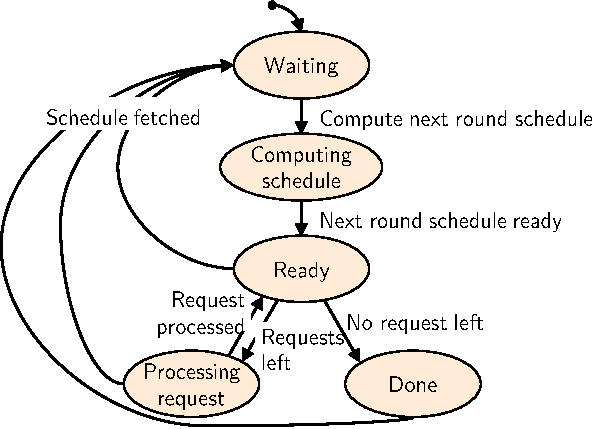
\includegraphics[scale=1]{AP_statemachine}
 \caption{State-machine of the host \AP.
 \capt{
  \AP first computes a valid schedule for the next round. Then, the \AP processes queued \DRP requests, one at a time, and recomputes a (new) schedule accounting for the newly admitted flow.
 }}
 \label{fig:AP_statemachine}
\end{figure}

\begin{figure}
 \centering
 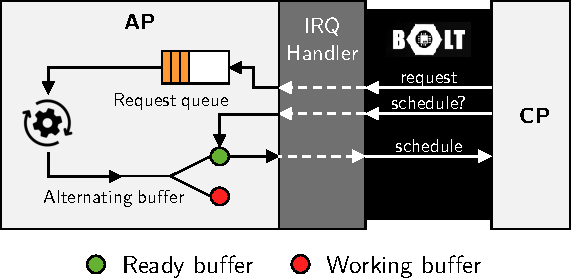
\includegraphics[scale=1]{AP_alternatingbuffer}
 \caption{Request queue and alternating buffer on the host \AP.
 \capt{
  Incoming messages from \CP trigger an interrupt and are handled immediately.
  \DRP requests are put in a dedicated queue for later processing~(\cref{fig:AP_statemachine}).
  When \CP writes a schedule request, the interrupt handler fetches the most recent schedule from the ``Ready buffer'' and write it to \bolt.
 }}
 \label{fig:AP_alternatingbuffer}
\end{figure}
}

\fakepar{Alternating buffers}
The host \CP fetches the next round schedule from its \AP, which sends a valid schedule immediately.
However, this conflicts with the admission of new flow requests: the \AP may be processing a request (including the computation of a new schedule) when \CP requests the schedule.

We handle this situation using an alternating buffer for the next round schedule~(\cref{fig:AP_alternatingbuffer}). One buffer is used to store a valid schedule for the next round, which the \AP computes first. After each \DRP request is processed, the newly computed schedule is written into the other buffer. The process repeats until all requests are processed.
%
Hence, even if \CP fetches while \AP is writing a schedule in one buffer, the other buffer still contains a valid schedule, which can be immediately sent to \CP over \bolt.
This guarantees a fast transmission of the schedule from \AP to \CP while avoiding memory corruption on the \AP.

\begin{remark}
  Alternative design choices and their respective benefits are further discussed in Andreas Biri's Master Thesis~\cite{biri2017Unleashing}.
\end{remark}

% !TEX root = ../00_thesis.tex

%-------------------------------------------------------------------------------
\section{Performance Evaluation}
\label{sec:drp_evaluation}
%-------------------------------------------------------------------------------

After detailing the design~(\cref{sec:designDetailed}) and implementation~(\cref{sec:drp_implementation}) of \DRP, we now evaluate the performance of the system. We consider three different performance aspects.

% However, \DRP provides hard guarantees based on a worst-case analysis, which is pessimistic by design. Thus, we investigate in this section the actual performance that \DRP can achieve.
\begin{itemize}
	\item
	First, we derive the theoretical optimal performances achievable by \DRP, based on the system model~(\cref{subsec:perf_model}).

	\item
	Then, we first use simulation to demonstrate the tightness of the worst-case analysis underlying \DRP's design: we show that end-to-end message latency reaches up to 97\% of the analytic bounds~(\cref{subsec:simulation}).

\pagebreak

	\item
	Finally, we showcase that our \DRP implementation performs as expected: all messages successfully transmitted through the wireless network do meet their end-to-end deadline. Furthermore, we illustrate that on a ``real'' network, messages typically experience latency much shorter than their end-to-end deadline~(\cref{subsec:flocklab}).
\end{itemize}


\begin{remark}
	The \triscale framework, introduced in \cref{ch:triscale}, would be beneficial for the design and analysis of \DRP's performance evaluation.
	However, the evaluation described below is anterior to the work we have done on \triscale, and thus does not use the framework.
\end{remark}


%-------------------------------------------------------------------------------
\subsection{Performance Model}
\label{subsec:perf_model}

The admission tests for \ap and \cp (which ensure that all contracts are satisfied after the admission of a new flow) critically depend on global parameters: the duration of a round \rlength and the deadline ratio $r$.

In this section, we analyze the influence of these parameters on the achievable performance of \DRP in terms of responsiveness (\ie the minimal admissible end-to-end deadline) and bandwidth.

\afterpage{
\begin{figure}
	\centering
	\href{\drpfig{Figure-10}}{%
	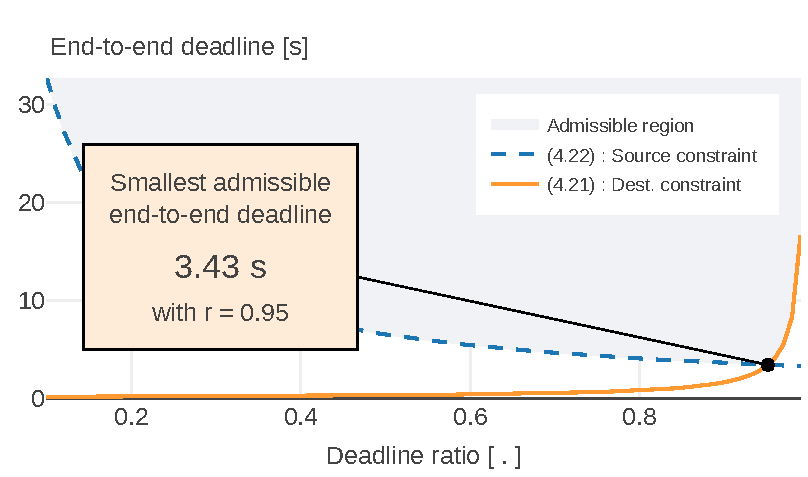
\includegraphics[scale=1]{min_e2edeadline}}
	\caption{The smallest admissible end-to-end deadline for $C_{net} = 1\s$ and $\tfdmin = 0.1\s$ is $\D_{min} = 3.43$\s.
	\capt{%
		Equations \eqref{eq:Dmin_destination_constraint} and \eqref{eq:Dmin_source_constraint} each define a feasible region for $(r,\deadlineany)$ tuples. The intersection defines the admissible region.}
	}
	\label{fig:min_latency}
\end{figure}}

%-------------------------------------------------------------------------------
\fakepar{Responsiveness: Minimal Admissible End-to-end Deadline}
Let us assume that the duration of communication rounds \rlength is given.
\DRP handles messages between application interfaces (\ie the \APs) and constrains the destination \apdst to flush \bolt (at least) every $T_f^d$. Naturally, there exists a lower bound on the admissible $T_f^d$; let us refer to this bound as \tfdmin.
Given these parameters, we are interested in the minimal admissible end-to-end deadline $\D_{min}$, or in other words, the maximal responsiveness of the protocol.

From the previous remark on $T_f^d$ and eq.  \eqref{eq:design_delay_destination} it follows
\begin{align}
\notag
	\tfdmin & \; \leq \; T_f^d \leq \left( (1-r)*\deadlineany - \delta_g^{const} \right)\\
\label{eq:Dmin_destination_constraint}
\Rightarrow \quad
	 \D & \; \geq \; \frac{\tfdmin +  \delta_g^{const}}{(1-r)}
%
\intertext{From \eqref{eq:ndeadline_constraint_latency} we also have}
%
\notag
 T + D + \overline{J}
	& \; \leq  \; r * \deadlineany - \delta_f^{const} \\
\notag
\Rightarrow \quad
	 \D & \; \geq \; \frac{T + D + \overline{J} + \delta_f^{const} }{r}
%
\intertext{%
We look for the minimal expression of the right-hand side term.
\eqref{eq:ndeadline_constraint_period} : $T_{net}^{min} \leq D_i \leq T_i$\; yields $T_{min} = D_{min} = T^{min}_{net}$.
Moreover, combining \eqref{eq:design_flush_period_source} and \eqref{eq:design_round_period} entails $T^{min}_{net} = T^s_f  = C_{net} + C_{CP}$. Hence $T_{min}$ is fixed given $C_{net}$.
Finally, in the best case, there is no (or small) jitter (\ie $\overline{J}=0$), and we obtain}
\label{eq:Dmin_source_constraint}
\Rightarrow \quad
	 \D & \; \geq \;	\frac{2T_{min} + \delta_f^{const}}{r}
\end{align}
\eqref{eq:Dmin_destination_constraint} and \eqref{eq:Dmin_source_constraint} define two lower bounds on the minimal admissible end-to-end deadline $\D_{min}$ induced by the contracts. Combining them, it follows that
\begin{align}
\notag &\D_{min} \;=\; \min_r
	\left(
	\frac{\tfdmin +  \delta_g^{const}}{(1-r)}
	\, , \,
	\frac{2T_{min} + \delta_f^{const}}{r}
	\right)
%
\intertext{The minimal value $\deadline{min}$ is reached for}
r_{opt} \;&=\; (2T_{min} + \delta_f^{const} )/(\tfdmin + \delta_g^{const} + 2T_{min} + \delta_f^{const})
%
\intertext{and it yields}
%
	&\D_{min} \;=\; \tfdmin + 2T_{min} + \delta_f^{const} + \delta_g^{const}
\end{align}

Using the parameters in \cref{table:simulation_parameters} from real-world prototypes, if $\rlength = 1$\s  and $\tfdmin = 0.1$\s, the minimal end-to-end deadline that can be supported is $\D_{min} = 3.43\s$, with $r = r_{opt} = 0.95$, and the minimum message interval $T = T_{min} = 1.074\s$. This case is illustrated in \cref{fig:min_latency}.
\TODO{rewrite as a table}


\begin{table}
\centering
\caption{Simulation parameters.
\capt{
	The \bolt API execution times are formally proven bounds for the given hardware~\cite{sutton2015Bolt}.
	The number of slots per round \nslotsmax is defined as the number of slots that ``fit'' into a round of length \rlength given the packet size.
	}}
{\smaller
\begin{tabular}{@{}c@{\qquad}l@{\qquad}c@{\qquad}l@{}}
\toprule
	&\textbf{Parameter}
	& \textbf{Symbol}
	& \textbf{Value} \\
\midrule
&WCET of \opwrite
	& $C_w$
	& $116 \us$\\
\bolt &WCET of \opread
	& $C_r$
	& $112 \us$\\
&WCET of \opflush
	& $C_f$
	& $684 \ms$\\
\midrule
&Round length
	&$C_{net}$
	& $1 \s$ \\
\blink &Packet size
	& $L$
	& $32$\bytes \\
&Max number of slots in one round
	&\nslotsmax
	& $46$ \\
\midrule
&Number of nodes
	& .
	& $20$ \\
\DRP &Deadline ratio
	& $r$
	& $0.5$ \\
&Flushing interval of $\cp$
	& $T_f^s$
	& $1.074 \s$ \\
\bottomrule
\end{tabular}}
\label{table:simulation_parameters}
\end{table}

%-------------------------------------------------------------------------------
\fakepar{Bandwidth: Maximal Duration of Communication Rounds}
Conversely, let us now assume that the minimal end-to-end deadline to be supported is given by $\D$, and consider the same assumption on $T_f^d$. The maximal bandwidth achievable by \blink is $\nslotsmax/T_{net}^{min}$ \pkts/\s. The round length $C_{net}$ is a linear function of the number of packets per round \nslotsmax (\ie a constant time per packet plus some overhead), and \linebreak
\eqref{eq:design_round_period} : $T_{net}^{min} = C_{net} + C_{CP}$. Hence, the maximal bandwidth actually grows with $C_{net}$. Thus, we now investigate the maximal admissible duration of communication rounds $C_{net}$ that yields the maximum available network bandwidth.

From \eqref{eq:ndeadline_constraint_latency} we have
$T + D + \overline{J}\;
	\leq  \; r * \deadlineany - \delta_f^{const}$, and, \linebreak
as previously, $T_{net}^{min} = C_{net} + C_{CP} \leq D \leq T$.
We get
\begin{align}
\label{eq:C_net_f(r)}
& C_{net}
		\;\leq\;
		 \frac{1}{2}
		 	(r * \deadlineany - \delta_f^{const}) - C_{CP}
%
\end{align}
From \eqref{eq:Dmin_destination_constraint}, given \deadlineany and \tfdmin, the maximal admissible value for $r$ is $\displaystyle r_{max} = 1 - ({\tfdmin + \delta^{const}_g}) / \deadlineany$ , and finally
\begin{align}
\label{eq:C_net_upperbound}
	& C_{net}
		\,\leq\,
		 \frac{1}{2}
		 	\left(
		 	\deadlineany - \delta_f^{const}- \delta_g^{const} - \tfdmin
		 	\right)
		 - C_{CP}
\end{align}

Using the parameters from \cref{table:simulation_parameters}, if we need to satisfy end-to-end deadlines of $\deadlineany = 10$\s and $\tfdmin = 3$\s, the maximal round length that can be supported is $\rlength = 2.82$\s, with $r = r_{max} = 0.69$, and the minimum message interval $T = C_{net} + C_{CP} = 2.89\s$. That upper-bound also yields the maximal achievable network bandwidth.
\TODO{rewrite as a table}

%-------------------------------------------------------------------------------
\fakepar{Effect of Deadline Ratio on System Performance}

We presented earlier that given $C_{net}$ and \tfdmin, there is an optimal value for $r$ that minimizes the admissible end-to-end deadline \deadlineany. If one tolerates ``larger'' deadlines, $r$ can be increased to allow for a bigger round length $C_{net}$ (see \eqref{eq:C_net_f(r)}), which increases the maximal network bandwidth.

However, \eqref{eq:design_delay_destination} yields $T_f^d \leq (1-r)*\deadlineany - \delta_g^{const}$. Hence, the bigger $r$ is the smaller $T_f^d$ must be, which may results in more flows rejected by the destination application.
On the contrary, if $r$ is set to its minimal value \linebreak
$\;r_{min} = ({2*T_{min} +  \delta^{const}_g})\, /\, {\deadlineany}$ (obtained from eq. \eqref{eq:Dmin_source_constraint}), it yields $T = \ndeadlineany = T_{min} = 1.074$\s and $\overline{J} = 0$\s. In other words, the maximal admissible jitter (obtained from \eqref{eq:jitter_bar}) is \linebreak
$J < T_f^s + C_r - C_f \approx 0.390$\s.
\TODO{space out a bit.}

How to set the parameters for \DRP depends on the application. For instance, if one consider an acoustic sensing scenario, responsiveness is usually quite critical, and the sensors (\ie the \APs) should spend most of their time on sensing, not being busy with flushing \bolt. Thus, we want to support a rather small $\D_{min}$ while having a strong constraint on \tfdmin. This will come at the cost of a "small" network bandwidth.

% !TEX root = ../00_thesis.tex


%-------------------------------------------------------------------------------
\subsection{Simulated Worst-Case Performance}
\label{subsec:simulation}

In \cref{subsec:perf_model}, we derived the optimal performance achievable according to our \DRP's model.
However, this model is based on a worst-case analysis of message latency throughout the system.
Because such an analysis is inherently pessimistic, it is important to estimate how pessimist the analysis is. In other words, how tight are the latency bounds given by the model?
In this section, we investigate this question using a discrete event simulation.

\fakepar{Procedure}
We simulate the run-time behavior of \DRP using the values and parameters from our implementations~(\cref{table:simulation_parameters}).
The simulation framework tracks the latency of each individual message through the entire system, \ie all \APs, \CPs, \bolt and the wireless communication network.
Concretely, the simulation is implemented using Matlab scripts (openly available -- \cref{append:drp_artifacts}).

\blink computes the round schedules assuming that the first message of each flow is available for communication at $t = 0\s$. The actual epoch at which the  \APs write the first packet of each flow is randomized between $0\s$ and the flow's minimal message interval $T$; subsequent packets are sent with period $T$.
The random seed is fixed for reproduciblility.

\fakepar{Scenario}
Node 1 acts as the sink and communicates with all other nodes in the network. As described in \cref{sec:designDetailed}, \DRP is initialized with a set of control flows $\mathcal{F}_{control}$, which is necessary in order to register subsequent flows
\[
\mathcal{F}_{control} =
	\left\lbrace
	\begin{tabular}{@{\,}l@{\,}}
	(1\,, n\,, \periodany = 10\s\,, \jitterany = 0\s\,, \deadlineany = 30\s )\\
	(n\,, 1\,, \periodany = 10\s\,, \jitterany = 0\s\,, \deadlineany = 30\s )\\
	\end{tabular}
	\right\rbrace
\]
for $n \in ($2$ .. $20$)$. In practice, such flows can also be used to send low-priority data (\eg status data) regularly to the sink.

An event from the environment (\eg a rock crack~\cite{meyer2019IPSN}) is co-detected by nodes 2 to 5, which consequently emit a request for a new flow to the sink node. In order to transfer the event data as fast as possible, the message interval is chosen as small as possible
(\ie equal to $T_f^s$, the flushing interval of $\cp$ -- Refer to \eqref{eq:design_flush_period_source}, \eqref{eq:design_round_period} and \eqref{eq:ndeadline_constraint_period}),
\[
\mathcal{F}_{new} =
	\left\lbrace
	\begin{tabular}{@{}l@{}}
	(n\,, 1\,, \periodany = 1.074\s\,, \jitterany = 0\s\,, \deadlineany = 10\s )\\
	\end{tabular}
	\right\rbrace
\]
for $n \in ($2$ .. $5$)$. We record the end-to-end latency of all packets during two minutes, during which about 900 messages are transmitted through the system.

\fakepar{Results}
\cref{fig:latency} shows the distribution of end-to-end latency of messages, shown as percentage of the analytical worst-case latency (given by \cref{thm:delta}).
We see that a few messages indeed experience a latency up to 97\,\% of the analytic worst-case bound.
The simulation also indicates that, in many cases, the worst-case buffer sizes of $\cp$ and \bolt are reached.
Overall, these results support our analysis of \DRP. They show that our worst-case bounds are tight; therefore, we can conclude that the performance derived using \DRP's model~(\cref{subsec:perf_model}) is representative of the performance that can be truly guaranteed by the system.


\begin{figure}
	\centering
	\href{\drpfig{Figure-11}}{%
	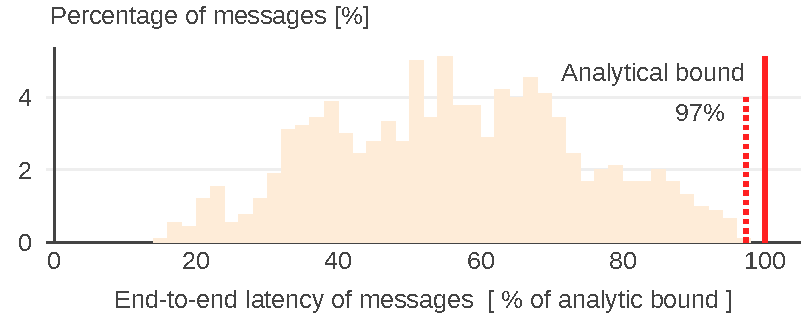
\includegraphics[scale=1]{lat_simu}}
	\caption{Distribution of end-to-end latency of messages, shown as percentage of the analytical worst-case latency.
		\capt{Some messages experience a latency very close to their worst-case bound (97\,\%), which demonstrates the tightness of the analysis.}
	 }
	\label{fig:latency}
\end{figure}

%-------------------------------------------------------------------------------
\subsection{Real-World Performance}
\label{subsec:flocklab}

\begin{table}
	\caption{Flow sets used in the end-to-end latency evaluation of \DRP.
	\capt{The \blink utilization is computed assuming a strictly periodic release of messages.}}
	{\smaller\input{\PathTab/flow_set.csv}}
	\label{tab:flow_set}
\end{table}

% Some intro about why we do real tests
We now consider the performance of our implementation of \DRP on embedded hardware: We use the first-generation DPP, which features a TI MSP432P401R as \AP and a TI CC430F5147 as \CP~(\cref{append:dpp}).
The software is based on the publicly available implementation of LWB~\cite{Code_LWB}; it is written in C and uses Contiki 2.7~\cite{contiki} as operating system.
The implementation of \blink on the \AP is built upon~\cite{acevedo2016Realtime}.
%
We discuss our implementation performance in terms of memory usage, computation workload, and message latency.

\fakepar{Memory usage}
\DRP requires both \AP and \CP to store some state information related to the currently running flows, as well message queues and buffers. The available RAM on both processors is shown in \cref{table:memory}.

The 64\kB of the \AP are largely sufficient; it would supports hundreds of flows. The \CP is more limited: With a payload size of 32\bytes, \CP is capped to a maximum for 40 flows~(\cref{table:memory}). For a regular node, this will likely be sufficient for most applications; however, on the host node, this seriously limits the scalability of the system.

One possible solution is to use the embedded external memory (128\kB); this would solve the memory limitation issue, but it may also introduce additional delays, which are currently not accounted for. Or we could use another processor as \CP with more than 4\kB of RAM.

\begin{table}
	\centering
	\caption{Memory available and required for our implementation of \DRP.
	\capt{%
		The difference between ``total'' and ``available''  memory corresponds to the memory taken by the firmware only. $L$ is the message payload.}
	}
	\label{table:memory}
	{\smaller\input{\PathTab/memory.csv}}
\end{table}


\fakepar{Computation}
The most extensive computations in \DRP are the computations of the \blink schedules and admission tests. The evaluation of these computations on embedded hardware is discussed in depth in~\cite{zimmerling2017Blink}.

In addition to \blink computations, the \APs must perform \DRP admission tests. These are simple operations~(\cref{thm:CP} and \ref{thm:AP}) which can be implemented efficiently. In our experiments, an admission test takes typically around 30\ms to complete (maximum observed execution time: 130\ms).

\DRP admission tests are performed only once per flow (when a new flow is requested). Thus, we can conclude that the computational workload induced by \DRP (in addition to \blink) is negligible.

\afterpage{
\begin{figure}
	\centering
		\begin{subfigure}{\linewidth}
				\captionsetup{labelformat=empty}
				\href{\drpfig{Figure-12}}{%
	      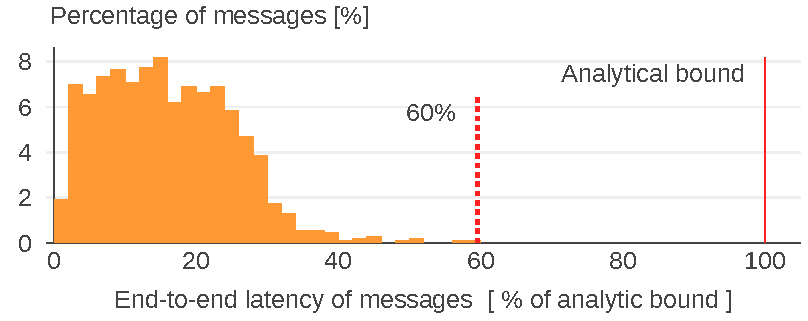
\includegraphics[scale=1]{lat_real_low}}
				\caption{}
			\end{subfigure}\\[10pt]
			\begin{subfigure}{\linewidth}
					\captionsetup{labelformat=empty}
					\href{\drpfig{Figure-12}}{%
		      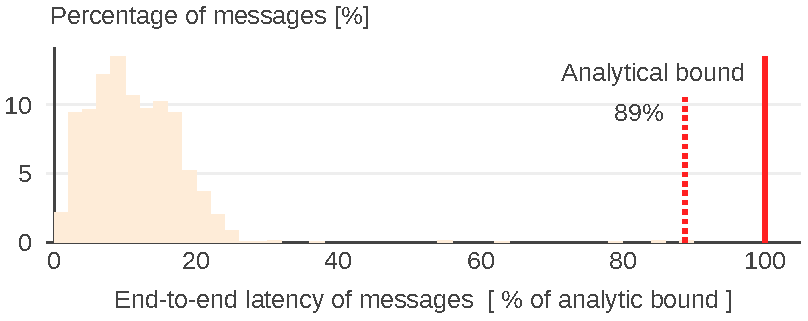
\includegraphics[scale=1]{lat_real_medium}}
					\caption{}
				\end{subfigure}\\[10pt]
				\begin{subfigure}{\linewidth}
						\captionsetup{labelformat=empty}
						\href{\drpfig{Figure-12}}{%
			      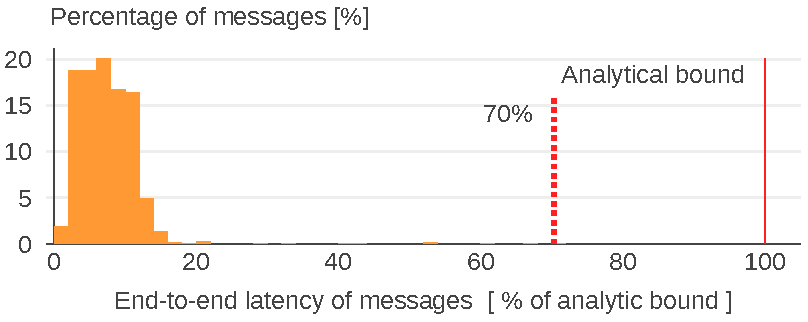
\includegraphics[scale=1]{lat_real_high}}
						\caption{}
					\end{subfigure}
  \caption{%
	Distribution of end-to-end latency of messages, shown as percentage of the analytical worst-case latency for a \DRP run using different flow sets~(\cref{tab:flow_set}).
	\capt{%
	Top -- Low utilization.
	Middle -- Medium utilization.
	Bottom -- High utilization.}
  }
  \label{fig:lat_real_all}
\end{figure}
}


\fakepar{End-to-end latency}
We investigate the experienced end-to-end latency of messages. We use a network of 10 source nodes and one host, and run experiments on the FlockLab testbed~\cite{lim2013FlockLab}. In addition to the control flows, each source node request a data flow toward the host with a pseudo-random period and end-to-end deadline.
Once the flow is admitted, the source \APs release new packets periodically.
The different flow sets used are listed in \cref{tab:flow_set}. \DRP is configured with a deadline ratio $r=0.5$, a round length $\rlength = 1\s$, and a maximum of $\nslotsmax = 5$ slots per round.


\begin{table}
	\centering
	\caption{Experienced latency of messages, expressed as percentage of the flow's end-to-end deadline.
	\capt{The tightness correspond to the ratio of the experienced latency with the analytical upper-bound given by~\cref{thm:delta}.}}
	{\smaller\input{\PathTab/latency.csv}}
	\label{tab:latency}
\end{table}


The results are summarized in \cref{tab:latency} and \cref{fig:lat_real_all}, reporting data from one run for each flow set.
The first observation is that all messages that are successfully transmitted over the wireless network do meet their end-to-end deadline.
However, compared to the simulation experiment~(\cref{subsec:simulation}), we do not encounter so much analytical corner cases: the observed latency is often much smaller than the analytical upper-bound~(\cref{fig:lat_real_all}).
On the other hand, this means that the actual runtime performance is better that what is guaranteed: even with large end-to-end deadlines (around 60\s), the experience message latency is most of the time between 5\s to 15\s.

Such ``short'' average latency can be explained by the nature of the flow set. The \emph{network} deadline, enforced by \blink, must be smaller than the flow period~\cref{sec:designDetailed}. Since the period are small compared to the \emph{end-to-end deadlines}, these end-to-end deadlines do not constraint the \DRP contracts: the experience latency correlates with the flow period.

It is interesting to observe that the average end-to-end latency is smaller for the high utilization flow set than for the low and middle ones. Again, this is due to the flow set. To meet the network deadline, \blink schedule at least one round per period. Thus, a flow set with shorter period results in more frequent rounds. Once a round is scheduled, it is filled with any message ready for transmission. Thus, flows are opportunistically served earlier than necessary to meet their end-to-end deadline. Conclusion: having a flow with a small period reduces the average latency experienced by all flows in the system. This is an interesting (and unforeseen) consequence of \DRP mechanism.

\fakepar{Conclusions}
The performance evaluation presented in this section validates the design of \DRP and our implementation: we showcased that we can run a wireless \CPS that meet end-to-end deadlines between distributed applications~(\cref{subsec:simulation} and \ref{subsec:flocklab}).
In addition, we derived the theoretical optimal performance achievable based on \DRP's model~(\cref{subsec:perf_model}).

A more thorough investigation of the actual system performance across different scenarios and environments remains to be performed.
For such a performance evaluation, using \triscale~(\cref{ch:triscale}) would be natural.

Chronologically, \triscale is the last piece of work of this dissertation. In hindsight, our evaluation of \DRP appears a bit naive and simple. Still, we argue that it successfully demonstrates the soundness of \DRP's design.% and supports our claims.

% !TEX root = ../00_thesis.tex
% \newpage

\pagebreak

\section{Related Work}
\label{sec:relWork}

Providing end-to-end guarantees in distributed networked systems has a long history in the context of the Internet. Notable developments are the resource reservation protocol (RSVP) that combines flow specification, resource reservation, admission control, and packet scheduling to achieve end-to-end quality of service~(QoS) \cite{zhang1993rsvp}. Network calculus \cite{cruz1991calculus} provides some of the necessary theoretical concepts to determine bounds on buffer sizes and delay in communication networks.
Extension toward hard real-time computing and communication systems is known as real-time calculus \cite{thiele2000Realtime}.
The analysis of distributed hard real-time systems also has a long history~\cite{tindell1994Holistic}, and so do compositional analysis frameworks (MAST~\cite{gonzalezharbour2001MAST}, SymTA/S \cite{henia2005System} and MPA~\cite{wandeler2006System}).

Early works on real-time communication in sensor networks consider classical non-deterministic routing protocols~\cite{lu2002RAP,stankovic2003Realtime,he2003SPEED}, thus providing only soft guarantees.
Stankovic et al. \cite{stankovic2003Realtime} even argue that specific message delivery orderings, such as those useful to apply established dependability techniques~\cite{ferrari2013Virtus}, are impossible to guarantee in a multi-hop low-power wireless network.
More recently, standards like WirelessHART~\cite{wirelessHART} have been analyzed to provide communication guarantees~\cite{saifullah2015EndtoEnd,saifullah2010RealTime}.
But~\cite{saifullah2010RealTime} is based on NP-hard multiprocessor scheduling and requires a global network view, which limits its adaptability to dynamic changes in the system~\cite{akerberg2011Measurements}.
It is however possible to integrate the wireless protocol with the rest of the system to avoid interference by jointly schedule transmissions in the network and all other tasks in the system, as we demonstrate in \cref{ch:ttw}.
Other wireless real-time protocols have been described recently~\cite{odonovan2013GINSENG,watteyne2017Teaching}. However, the integration of these protocols into a methodology to provide end-to-end real-time guarantees between \emph{application interfaces} is unsolved.

\squarepar{%
  Recently, a game-changing approach to wireless multi-hop communication using synchronous transmissions has been described~\cite{ferrari2011Glossy,ferrari2012LWB,zimmerling2013modeling}.
  It avoids the computation of multi-hop routing paths and per-node communication schedules based on, for example, neighbor lists and link qualities, because the protocol logic is independent of such volatile network state.
  Experiments on several large-scale testbeds show that the approach is highly adaptive and achieves an end-to-end packet reliability higher than 99.9\,\%~\cite{ferrari2011Glossy,ferrari2012LWB}.
  Furthermore, the few packet losses can be considered statistically independent~\cite{zimmerling2013modeling}, which eases the design of \CPS controllers that can deal with intermittent observations~\cite{sinopoli2004Kalman}.%
}

% !TEX root = ../00_thesis.tex
% \pagebreak
\newpage
\section{Summary}

%What we presented
In this chapter, we presented the \DRPLong (\DRP), a global system design that provides end-to-end real-time guarantees between interfaces of distributed applications in wireless \CPS.
\DRP meets the requirements of \feature{Timeliness}, \feature{Reliability}, \feature{Adaptability}, and \feature{Composability}.
However, since \DRP guarantees relies on worst-case analysis, the system's \feature{Efficiency} is inherently limited; still, we demonstrated that our analysis is tight~(\cref{sec:drp_evaluation}) which shows that \DRP is not overly pessimistic.

% Key concept/novel idea
The key concept of \DRP is to (i)~physically decouple the communication protocol from the application tasks (each running on dedicated communication and application processors), and (ii)~guarantee the timeliness of message transmissions throughout the system using minimally restrictive contracts between the different entities.

% Take aways
We implemented and ran a proof-of-concept implementation of \DRP on embedded hardware.
The firmware source code as well as our \DRP simulation framework are openly available~(\cref{append:drp_artifacts}).
\DRP appears to be a promising solution for low-rate applications, such as smart homes, where  coexists multiple context-specific ``applications'' (\eg fridge, air-conditioning, lightning) which would particularly benefit from being scheduled independently from each other while being able to communicate in real-time.


% Chapter appendices
\begin{subappendices}

\newpage
% !TEX root = ../00_thesis.tex
\section{Appendix -- Artifacts and Links}
\label{append:baloo_artifacts}

\subsection{Related Publications}

\inlineRef%
{Synchronous Transmissions Made Easy: Design Your Network Stack with Baloo}%
{Romain Jacob, Jonas Bächli, Reto Da Forno, Lothar Thiele}%
{EWSN 2019. Beijung, China (February 2019)}

\customLink{\faFileTextO}{Paper}{10.3929/ethz-b-000324254}{https://doi.org/10.3929/ethz-b-000324254}
\customLink{\faDesktop}{Presentation}{10.3929/ethz-b-000328814}{https://doi.org/10.3929/ethz-b-000328814}

\inlineRef%
{Creating a Flexible Middleware for Low-Power Flooding Protocols}%
{Jonas Bächli}%
{Master Thesis. ETH Zurich (June 2018)}

\customLink{\faBook}{Thesis}{10.3929/ethz-b-000270388}{https://doi.org/10.3929/ethz-b-000270388}

\subsection{Complementary Materials}
Complementary materials for this chapters are available on GitHub, together with the dissertation source files. For all links below, replace\\
\linkroot  by ``{github.com/romain-jacob/doctoral-thesis/blob/master}''

\customLink{\faFilesO}{\tex sources}{\linkroot/30\_Baloo/}{\linkrootURL/30\_Baloo/}
\customLink{\faFileImageO}{Figures}{\linkroot/30\_Baloo/Figures/}{\linkrootURL/30\_Baloo/Figures/}
% \customLink{\faCopyright}{\credit}{\linkroot/credits/30\_Baloo.pdf}{\linkrootURL/credits/30\_Baloo.pdf}
\customLink{\faGlobe}{Webpage}{romainjacob.net/baloo}{http://www.romainjacob.net/research/projects/baloo/}
%
\customLink{\faCode}{\baloo source code}{}{}
  \customLink{}{--- Documentation}{GitHub Wiki}{https://github.com/ETHZ-TEC/Baloo/wiki}
  \customLink{}{--- Latest release}{10.5281/zenodo.3510171}{https://doi.org/10.5281/zenodo.3510171}
  \customLink{}{--- ``This-version'' release}{10.5281/zenodo.3530632}{https://doi.org/10.5281/zenodo.3530632}
\customLink{\faChain}{Experiment data}{}{}
  \customLink{}{--- Latest release}{10.5281/zenodo.3510198}{https://doi.org/10.5281/zenodo.3510198}
  \customLink{}{--- ``This-version'' release}{10.5281/zenodo.3510214}{https://doi.org/10.5281/zenodo.3510214}


\newpage
% !TEX root = ../00_thesis.tex

%-------------------------------------------------------------------------------
\section{Appendix -- Worst-case Latency Analysis}
\label{append:drp_WCanalysis}
%-------------------------------------------------------------------------------

%\subsubsection{Worst-case analysis of the source delay}
\fakepar{Worst-case analysis of the source delay}
\begin{definition}[Source delay -- $\delta_{source}$]
The source delay is the elapsed time from
a packet being written in \bolt by the source \apsrc
until
the end of the \opflush operation where it is read out of \bolt by the source \cpsrc.
For a flow \flowi, it is denoted by $\delta_{source, \,i}$.
\end{definition}

\begin{lemma}\label{lem:delta_source}
For any flow \flowi, the source delay is upper-bounded by
\begin{equation}
\label{eq:delta_source}
\delta_{source, \,i} \; \leq \; C_w + T_f^s + C_f
\end{equation}
\end{lemma}

\begin{proof}%
Let us recall that a \opflush is a sequence of \opread operations. When the \bolt queue is found empty, the \opflush is terminated and no other \opread is performed until the next \opflush (refer to \ref{subsec:boltAPI} for details).
Therefore, if the \bolt queue is empty and a \opwrite operation terminates just after a \opflush is triggered, that \opflush immediately terminates and the packet is delayed until to the end of the next \opflush.
Possible jitter on the \opwrite operation pattern does not have any influence on the worst-case for $\delta_{source, \,i}$.
This worst-case scenario for the source delay is illustrated on Fig.~\ref{fig:delta_source_time_graph}. \
\end{proof}

\begin{figure}[h!]
\centering
\includegraphics[scale=1]{delta_source_time_graph}
\caption{Worst-case analysis of the source delay.
\capt{A packet is written as early as possible such that it misses a \opflush and must wait until the next one.}}
\label{fig:delta_source_time_graph}
\end{figure}


%%%%%%%%%%%%%%%%%%%%%%%%%%
%%%%======================
%%%%%%%%%%%%%%%%%%%%%%%%%%


\fakepar{Worst-case analysis of the network delay}
\begin{definition}[Network delay -- $\delta_{network}$]
The network delay is the elapsed time from
a packet being available for communication at the source \cpsrc
until
the end of the communication round where it is served by the wireless protocol (i.e., when it is available at the destination \cpdst).
For a flow \flowi, it is denoted by $\delta_{network, \,i}$.
\end{definition}

\begin{lemma}\label{lem:delta_network}
For any flow \flowi, the network delay is upper-bounded by
\begin{equation}
\label{eq:delta_network}
\delta_{network, \,i} \; \leq \; T_i + D_i + \floor*{\frac{\jitteri + C_f - C_r}{T_f^s}}\cdot T_f^s
\end{equation}
\end{lemma}
\begin{proof}%
As presented in \cref{subsec:details_blink}, \blink guarantees that every packet matching the \emph{expected arrival} is served in a round that terminates before the network deadline $D_i$; \ie the \emph{delay of an expected packet} is no more than $D_i$.

However, the actual arrival of packets at the source \cpsrc does not match the expected arrival in general, but results from \opflush operations, which occur every $T_f^s$ time unit.
Hence, a packet may arrive \emph{earlier} than the next expected packet. That mismatch between the two arrival times (actual and expected) adds up with the delay of the expected packet (i.e., $D_i$).

Let us consider first that the flow \flowi has no jitter (\ie $\jitteri =0$) and let $m$ be the mismatch between actual and expected arrival time at \cpsrc. $m$ cannot be larger than the flow's minimum message interval $\periodi$
\[
m \;\leq\; \periodi
\]
The intuition is given with \cref{fig:delta_network_time_graph1}. See the caption for details.

\begin{figure}[h!]
\centering
\includegraphics[scale=1]{delta_network_time_graph1}
\caption{Worst-case analysis of the network delay without jitter.
\capt{Because of the \bolt queue being empty, packet \textbf{A} misses the first flush operation (similarly as in \cref{fig:delta_source_time_graph}), hence the slot allocated to \flowi in round \textbf{1} is wasted. Due to packets released from other flows in the meantime, packet \textbf{B} is flushed directly in the operation preceding round \textbf{3}, in which flow \flowi is allocated a new slot. However, as packet \textbf{A} is still in queue, packet \textbf{B} is not served right away but is delayed until the next allocated slot (\ie in round \textbf{6}). This creates a mismatch of \periodi for packet \textbf{B}.
Furthermore, the mismatch cannot get bigger; assume \textbf{B} were to be available at \cpsrc earlier (\ie one flush operation before, at least), because the time interval between \textbf{A} and \textbf{B} must be at least \periodi, \textbf{A} would arrive earlier as well.
Hence, \textbf{A} would not miss the slot in round \textbf{1}, \textbf{B} would be served in round \textbf{3},
and thus it would yield a smaller mismatch for packet \textbf{B}.}}
\label{fig:delta_network_time_graph1}
\end{figure}


Now, if flow \flowi has also jitter \jitteri, this may entail a bigger mismatch. Actual "arrival" of packets (\ie the epoch when a packet is available for communication at the source \cpsrc, according to the definition of the network delay) can occur only every $T_f^s$ (\ie at the end of one \opflush operation). Therefore, one can see that jitter may induce an extra delay, or mismatch, of roughly $\floor*{\jitteri/T_f^s}\cdot T_f^s$. A more precise analysis of the flushing dynamics (see \cref{fig:delta_network_time_graph2} for details) entails that, overall, the worst-case mismatch $m$ is bounded by

\begin{align}
\label{eq:mismatch}
m \; \leq \;\; &
	T_i + \floor*{\frac{\jitteri + C_f - C_r}{T_f^s}}\cdot T_f^s\\
\intertext{and finally,}
\notag
\delta_{network, \,i} \; \leq \;\; &
	D_i + m \\
\notag
\delta_{network, \,i} \; \leq \;\; &
	T_i + D_i + \floor*{\frac{\jitteri + C_f - C_r}{T_f^s}}\cdot T_f^s \quad \
\end{align}
\end{proof}

\begin{figure}[h!]
\centering
\includegraphics[scale=1]{delta_network_time_graph2}

\caption{Influence of jitter on the network delay.
\capt{Let us have a closer look at packet \textbf{B} from the previous figure, positioned as early as possible (\ie if it were earlier, so would be \textbf{A}, which would then not miss its slot in round \textbf{1}).
Due to jitter, \textbf{B} is released earlier, say by a amount $j$. This can yield packet \textbf{B'} (\textbf{B} with jitter) to be read out in a previous \opflush operation. In the worst-case, packet \textbf{B'} is read out one operation earlier as soon as $j$ is bigger than $T_f^s - C_f + C_r$, which increases the mismatch $m$ by $T_f^s$. Similarly, $m$ increases by $k \cdot T_f^s$ when $j$ reached  $k \cdot T_f^s - C_f + C_r$, which yields $k = \floor*{\frac{j + C_f - C_r}{T_f^s}}$ and concludes to equation \eqref{eq:mismatch}.
}}
\label{fig:delta_network_time_graph2}
\end{figure}






%%%%%%%%%%%%%%%%%%%%%%%%%%
%%%%======================
%%%%%%%%%%%%%%%%%%%%%%%%%%

\fakepar{Worst-case analysis of the destination delay}

\begin{definition}[Destination delay -- $\delta_{dest}$]
The destination delay is the elapsed time from
a packet being available at the destination \cpdst
until
the end of the \opflush operation where it is read out of \bolt by the destination \apdst (i.e., when it is available for the application).
For a flow \flowi, it is denoted by $\delta_{dest, \,i}$.
\end{definition}


\newpage
\noindent

\begin{lemma}\label{lem:delta_destination}
For any flow \flowi, the destination delay is upper-bounded by
\begin{equation}
\label{eq:delta_destination}
\delta_{dest, \,i} \; \leq \; \nslotsmax*C_w - (\nslotsmax-1)* C_r + T_f^d + C_f
\end{equation}
\end{lemma}

\begin{proof}
The situation is similar as for the source delay, except
that \cpdst writes every $T_{net}$ time unit (\ie after each round) all the packets it received during the last round, which can be as many as \nslotsmax packets.
%\cp writes packets to \bolt sequentially after each communication rounds, where they stay until they are flushed out by AP.
The maximal delay for a packet occurs when it is written too late to be read out during an ongoing \opflush and must wait for the next one.

A careful analysis of the \bolt dynamics shows that the \opread operation is slightly shorter than \opwrite \cite{sutton2015Bolt} (i.e., $C_r < C_w$, see Table \ref{table:simulation_parameters}). Hence, the more packets are written at once by \cpdst, the later a \opflush can start and still miss the last written packet. The worst-case is illustrated on Fig.~\ref{fig:delta_destination_time_graph}. \
\end{proof}

\begin{figure}[h!]
\centering
\includegraphics[scale=1]{delta_destination_time_graph}
\caption{Worst-case analysis of the destination delay.
\capt{A packet is written as early as possible such that it misses a \opflush and must wait until the next one.}}
\label{fig:delta_destination_time_graph}
\end{figure}



\end{subappendices}

% !TEX root = ../00_thesis.tex
\clearpage

\TODO{
TTW
\begin{itemize}
  \item carefully check theorem 1.1 proof.
  \item comment on preemptive schedule for the tasks
\end{itemize}
}

\chapter[\TTW~-- Time-Triggered Wireless]{\TTW: A Time-Triggered Design for Wireless Cyber-Physical Systems}
\label{ch:ttw}

\renewcommand{\ChapPath}{50_TTW}
\renewcommand{\TablePath}{50_TTW/Tables}

% !TEX root =  ../00_thesis.tex

% ------------------------------------------------------------------------------
% Global Positioning
In the previous chapter, we discussed how to design and analyze networking experiments in general~(\cref{ch:triscale}).
In the rest of this dissertation, we will focus on low-power wireless networking, and more specifically on a technique called \emph{synchronous transmissions}.

% ------------------------------------------------------------------------------
% Context
Synchronous transmissions (\ST) refers to a wireless approach for broadcasting messages in a multi-hop network using flooding.
This is made efficient by letting multiple transmitters send the \emph{same packet} at the \emph{same time}; hence the name of \emph{synchronous} transmissions.%
\footnote{The name \textsl{concurrent transmissions} is also found in the literature.}
\ST has been proven highly reliable and energy efficient for low-power wireless networks.
Furthermore, \ST supports mobility by design thanks to the stateless logic of flooding-based communication.

% ------------------------------------------------------------------------------
% What is the problem?
Unfortunately, it is difficult to guarantee that multiple nodes actually send at the ``same time''.
The required precision on synchronization depends, \eg on the physical layer speed, the radio modulation speed or the encoding scheme.
For typical low-power wireless motes available today, the synchronization must be in the order of \us for \ST to work reliably.
Achieving such time synchronization requires to precisely control the timing of radio operations, which involves careful timer settings and interrupt handling.
The integration of such ``low-level software'' within a entire network stack is challenging.
Consequently, the adoption and development of \ST-based network stacks has been hindered by
the lack of usable and flexible design tools.

\begin{figure}
  \centering
  \includegraphics[scale=0.9]{chapter_baloo}
  \caption{Positioning of this chapter in the dissertation.
  \capt{This chapter presents \baloo, a design framework facilitating the implementation of low-power wireless networking protocols based on synchronous transmissions.}}
  \label{fig:chapter_baloo}
\end{figure}

% ------------------------------------------------------------------------------
% Claim
Thus, in this chapter, we study the feasibility of a design tool that would facilitate the development of network stacks based on \ST~(\cref{fig:chapter_baloo}); typically, such a tool would be useful for implementing our real-time protocol stacks (see \cref{ch:drp} and \cref{ch:ttw}).

\fakepar{Claim}
We propose and implement \baloo, a design framework for network stacks based on synchronous transmissions.
\baloo significantly lowers the entry barrier for harnessing the efficiency, reliability and mobility support of synchronous transmissions: users implement their protocol through a simple yet flexible API while \baloo handles all the complex low-level operations based on the users' inputs.

\baloo is flexible enough to implement a wide variety of network layer protocols, with only limited memory and energy overhead.

% ------------------------------------------------------------------------------
% Corresponding reference(s)
\begin{publi}

  The material from this chapter builds upon the work from Jonas Bächli~\cite{bachli2018Creating}. It relates to the following publication.

  \inlineRef{Synchronous Transmissions Made Easy: Design Your Network Stack with Baloo}{Romain Jacob, Jonas Bächli, Reto Da Forno, Lothar Thiele}{EWSN 2019. Beijung, China (February 2019)}

\end{publi}

% ------------------------------------------------------------------------------
% ------------------------------------------------------------------------------
% FORMER INTRO
% ------------------------------------------------------------------------------
% ------------------------------------------------------------------------------
% \newpage
% %Context
% \textsl{Synchronous Transmissions} (\ST) refers to a wireless communication technique that broadcast messages in a multi-hop network using flooding.
% This is made efficient by letting multiple transmitters send the \textsl{same packet} at the \textsl{same time}; henceforth the name of \emph{synchronous} transmissions.%
% \footnote{The name \textsl{concurrent transmissions} is also found in the literature.}
% \ST has been proven to be highly reliable and energy efficient, in particular for low-power wireless networks. Furthermore, flooding allows \ST to seamlessly support mobility by design.
% More informantion about \ST are presented in Introduction (\cref{ch:introduction}).
%
% %Problem
% Unfortunately, it is difficult to guarantee that multiple nodes actually send at the ``same time''.
% The required precision on synchronization depends \eg on the physical layer speed, the radio modulation speed or the encoding scheme.
% For typical low-power wireless motes available today, the synchronization must be in the order of \us for \ST to work reliably.
% Achieving such time synchronization requires to precisely control the timing of radio operations, which involves careful timer settings and interrupt handling.
% The integration of such ``low-level software'' within a entire network stack is challenging.
% Consequently, the adoption and development of \ST-based network stacks has been hindered by
% the lack of usable and flexible design tools.
%
% %Task and object
% Therefore, we developed \baloo: a flexible network stack design framework, designed to facilitate the development of protocols based on \ST. The key element of \baloo is a middleware layer which separates the radio management from the protocol implementation: \baloo provides a flexible application programming interface, while ensuring the correct timing of radio operations.
%
% %Findings
% \baloo is flexible enough to implement a wide variety of network layer protocols, with only limited memory and energy overhead.
% Most importantly \baloo makes \ST accessible: The software is open source and well documented.
% Since its development, \baloo has been used in a variety of projects, from both our team and external research groups.
% We believe that \baloo is an important enabler for a whole new class of Internet of Things applications leveraging the reliability, efficiency, and flexibility of \ST.

%
%
% This chapter presents \baloo, its design and the evaluation of its performance. We conclude with a brief description of projects that have been facilitated by \baloo, and finally discuss potential future developments, including standardization efforts.

% !TEX root =  ../00_thesis.tex

\section{Prolem Setting}
\label{sec:baloo_intro}

\squarepar{%
  Synchronous Transmissions (\ST) is an increasingly used wireless communication technology for low-power multi-hop networks. Popularized by Glossy~\cite{ferrari2011Glossy} in 2011, it has been proven to be highly reliable and energy efficient, as illustrated by the EWSN Dependability Competition ~\cite{schuss2017Competition}, where all wining solutions were based on \ST~\cite{escobar2018Competition,sommer2016Competition,lim2017Competition, escobar2019RedNodeBus, ma2019DeCoT} in the past four years (2016 to 2019).%
}

A \textsl{\ST primitive} refers to a protocol that efficiently realizes broadcast (\ie any-to-all communication) in bounded time, usually relying on \textsl{flooding}.
Flooding is a communication strategy that realizes broadcast by having all receivers of a packet retransmit this same packet to all their neighbours; the packet is thus ``flooded'' through the whole network. \ST makes flooding energy and time efficient by letting multiple wireless nodes transmit the packet \textsl{synchronously}, hence the name of \textsl{Synchronous Transmissions}. The successful reception of the packet can be achieved if the transmitters are tightly synchronized, thanks to \textsl{constructive interference} and the \textsl{capture effect}~\cite{yuan2013LetTalkTogether}.
The synchronization requirements vary from sub-\us to tens of \us, depending on the platform and modulation scheme~\cite{yuan2013LetTalkTogether}.
 %
%\footnote{Some background on flooding and \ST technology is provided in \cref{sec:baloo_overview}.}.
Such a broadcast primitive simplifies the design of network layer protocols: The underlying multi-hop network can be abstracted as a \textsl{virtual single-hop network} and thus be scheduled like a shared bus~\cite{ferrari2012LWB}.
One may refer to \cref{ch:introduction} for more details on \ST.

Since Glossy~\cite{ferrari2011Glossy}, many flavours of \ST primitives have been proposed to improve performance in terms of reliability, latency, and energy consumption.
To be more resilient to strong interference, Robust Flooding~\cite{lim2017Competition} is a primitive that modifies the RX-TX sequence from the original Glossy, whereas RedFixHop~\cite{escobar2016RedFixHop} uses hardware acknowledgements to minimize the number of retransmissions required.
Instead, some primitives aim to minimize latency for specific traffic patterns.
For example, Chaos~\cite{landsiedel2013Chaos} lets all nodes modify the packet being flooded to quickly aggregate information (\eg the max value of all sensor readings) or efficiently perform all-to-all data sharing to achieve distributed consensus~\cite{alnahas2017a2}.
Codecast~\cite{mohammad2018Codecast} also targets many-to-many exchange for a larger amount of data.
Pando~\cite{du2015Pando} is another primitive focused on high throughput, which uses fountain code and packet pipelining for efficient data dissemination.
Syncast~\cite{mohammad2017Improving} aims to reduce the radio on time required to save energy, while Less is More (LiM)~\cite{zhang2017LiM} is a primitive that reduces energy consumption using learning to avoid unnecessary retransmissions during flooding.

\squarepar{%
  All these primitives share the same drawback: Successful \ST requires low-level control of timers and radio events in order to meet \ST tight synchronization requirements (the order of \us).
  This degree of accuracy is difficult to achieve as it requires a detailed knowledge of the underlying hardware, low-level control of the radio operations, and a very careful management of software delays.%
}

As a result, designing a network stack based on \ST is a complex and time consuming task, for which only few solutions have been proposed.
One of the first was the Low-power Wireless Bus (LWB) ~\cite{ferrari2012LWB}, which tries to flexibly support all kinds of traffic patterns in a balanced trade-off between latency and energy consumption.
The same group designed eLWB~\cite{sutton2017eLWB}, a variation of LWB tailored to event-based data collection.
Sleeping Beauty~\cite{sarkar2016Sleeping} was later proposed to minimize energy consumption for data collection scenarios with many redundant sensor nodes.
Time-Triggered-Wireless (TTW -- \cref{ch:ttw})~\cite{jacob2017TTW_extended} was designed to minimize the end-to-end latency between communicating application tasks.
Finally, Crystal~\cite{istomin2018Interferenceresilient} has been proposed as a network stack specialized for sporadic data collection.
All these network stacks solely rely on Glossy as \ST primitive.
%
In principle however, the same protocol logic could benefit from \textsl{multiple} primitives. For example, an LWB network could use Robust Flooding~\cite{lim2017Competition} in case of high interference, then revert to Glossy~\cite{ferrari2011Glossy} for better time synchronization. If nodes need reprogramming, the software update can be quickly disseminated using Pando~\cite{du2015Pando}.
Designing a modular network stack supporting multiple \ST primitives adds a new level of complexity.

\begin{research_questions}
  \begin{description}
    \item[Question 1]
    Can we facilitate the design of wireless network stacks based on Synchronous Transmission?

    \item[Question 2]
    Can we implement flexible and adaptive protocols, potentially leveraging multiple \ST primitives, while guaranteeing that the timing requirements of \ST are met?
  \end{description}
\end{research_questions}

\fakepar{The problem}
To facilitate the network stack design (\question{1}),
a natural idea is to separate the concern of the timely execution of the primitives from the implementation of the protocol logic.
One way to achieve such separation of concerns is to use a \textsl{middleware} as part of the network stack.

%Challenges
The idea of a middleware for Wireless Sensor Networks (WSN) is not new, and the main challenge in such an endeavour is well-known.
As phrased by Mottola and Picco~\cite{mottola2012Middleware}, ``\textit{striking a balance between flexibility and complexity in providing access to low-level features is probably one of the toughest, yet most important, problems in WSN middleware}''.

The design of a middleware for \ST is particularly challenging.
Indeed, meeting the tight timing requirements for \ST is directly conflicting with the concept of abstraction of a middleware: How to guarantee that the network layer does not hinder the timing accuracy for \ST if it is itself unaware of the execution of the primitives? That is \question{2}.


\fakepar{The challenge} A middleware for \ST should meet the following requirements.
% This problem can be formulated by the following challenges:

\begin{features}

	\item[Usability]
	The middleware must realize a well-defined interface enabling runtime control from the network layer (which implements the protocol logic) over the execution of the underlying \ST primitives.

	\item[Generality]
	The middleware must enable the implementation of a large variety of network layer protocols.

	\item[Versatility]
	The middleware must enable one network layer protocol to use multiple \ST primitives and switch between them at runtime.

	\item[Synchronicity]
	The middleware must guarantee to respect the time synchronization requirements for \ST (from sub-\us to tens of \us~\cite{yuan2013LetTalkTogether}).
\end{features}

\pagebreak
%Task/Contibution
\fakepar{Our solution}
To address these challenges, we have designed \baloo, a flexible design framework for low-power network stacks based on \ST.%
\footnote{The framework provides the ``bare necessities'' for the design and implementation of \ST-based network stacks; so we called it \baloo.}
\baloo provides a large set of features enabling performant protocol designs, while abstracting away low-level hardware management such as interrupt handling and radio core control.
In summary:

\begin{itemize}
	\item
	We propose \baloo, a flexible design framework for low-power wireless network stacks based on \ST, illustrated in \cref{fig:stack_baloo}.

	\item
	We present the design of a middleware layer that meets all our requirements. This middleware forms the core component of \baloo.

	\item
	We showcase the usability of \baloo by re-implementing three well-known network stacks using \ST: the Low-power Wireless Bus (LWB)~\cite{ferrari2012LWB}, Sleeping Beauty~\cite{sarkar2016Sleeping}, and Crystal~\cite{istomin2018Interferenceresilient}.

	\item
	We illustrate the portability of \baloo by providing implementations for two platforms -- the CC430 SoC~\cite{CC430F6137} and the old but still heavily used TelosB mote~\cite{TelosB}.

	\item
	We demonstrate that \baloo induces only limited performance overhead (memory usage, radio duty cycle) compared to the original implementations.

\end{itemize}


\begin{figure}
  \includegraphics[scale=1]{stack_baloo.pdf}\\~\\
  \begin{minipage}[t]{.47\linewidth}
    \textbf{(a)} The implementation of the network layer protocol (Crystal) couples the interface to the underlying \ST primitive (Glossy) and the protocol logic, \ie how long are the communication rounds, which radio channel is used, \etc
  \end{minipage}
  \hfill
  \begin{minipage}[t]{.47\linewidth}
    \textbf{(b)} Thanks to its additional middleware layer, \baloo flexibly supports multiple \ST primitives and significantly reduces the efforts required to implement  network layer protocols compared to traditional stacks, like LWB~\cite{ferrari2012LWB} or Crystal~\cite{istomin2018Interferenceresilient}.
  \end{minipage}
  %
  \caption{Crystal~\cite{istomin2018Interferenceresilient} is a typical example of network stack based on \ST (\cref{fig:stack_baloo}a).
		Conversely, \baloo is a flexible design framework.
		It is based on a middleware layer that separates the concern of timely execution of \ST primitives from the implementation of the protocol logic (\cref{fig:stack_baloo}b).}
	\label{fig:stack_baloo}
\end{figure}

This chapter \emph{is not} meant to cover all details and inner mechanisms of \baloo, but mainly presents the core concepts of the framework.
\baloo is open source and the complete technical documentation is available online~(\cref{append:baloo_artifacts}).

% !TEX root = ../00_thesis.tex

\begin{figure}
	\centering
	\includegraphics[scale=1]{ttw_overview}
	\caption{Overview of \TTW.
		\capt{Nodes execute distributed \CPS applications. They communicate over a multi-hop wireless network using Glossy floods~\cite{ferrari2011Glossy}.
		Communication is organized in \TTnet rounds~(\cref{fig:ttnet}) which are controlled by a central host (running on one of the nodes).
		\TTW is a global scheduler for the entire system: it co-schedules the execution time of all tasks and messages in order to reduce the end-to-end latency of applications and meet short deadlines.}
	}
	\label{fig:ttw_overview}
\end{figure}


% \caption{(a) General system model and (b) time-slotted execution of \TTW.
% \capt{%
% As in LWB\emph{~\cite{ferrari2012LWB}}, communication rounds are divided into time slots, in which Glossy floods are executed. Each color shows one flooding step.
% In \TTW, the first slot of each round contains a beacon sent by the host, followed by (up to) \nslotsmax slots, allocated to application messages. The beacons announce the identification number of the round (round \id) and trigger mode changes.
% }

\section{Overview of \TTW}
\label{sec:ttw_overview}

We first present \TTnet, a network stack based on synchronous transmissions (\ST), which serves as communication backbone for our solution~(\cref{subsec:ttnet}). We then introduce the concepts of \TTW~(\cref{subsec:ttw_concepts}), a system-wide scheduler built atop \TTnet to realize a wireless \CPS solution meeting the requirements described above.

\subsection{The \TTnet communication backbone}
\label{subsec:ttnet}

We consider a set of nodes connected by a wireless multi-hop network~(\cref{fig:ttw_overview}).
Each node is a low-power embedded device, typically battery-powered, with limited computational resources such as memory or processing power.
These devices collectively implement distributed applications (\eg closed-loop control). These applications are composed of multiple tasks and messages; the tasks are executed locally by the nodes; the messages are exchanged over the multi-hop wireless network.
In low-power wireless \CPS, a significant part of the energy is consumed by wireless communication. Thus, to minimize the energy consumption, we group messages into communication rounds, \ie time intervals where all nodes turn their radio on and communicate.
Each round is composed of dedicated time slots where nodes communicates using Glossy, a flooding protocol which delivers packets with a probability above 99.9\,\%~\cite{ferrari2011Glossy}.
The system is controlled centrally by a node called the host, which sends commands at the beginning of each round in a special slot called beacon.
Physically, one of the nodes plays the role of the host.
We call this network stack \TTnet~(\cref{fig:ttnet}).


\begin{figure}
	\centering
	\includegraphics[scale=1]{ttnet}
	\caption{The \TTnet network stack.
	\capt{%
		\TTnet organizes communication in time-triggered rounds, between which nodes turn their radio off to save energy.
		The rounds are composed of (up to) \nslots communication slots preceded by a beacon, sent by the host to distribute runtime control information.
		In each slot, an one-to-all communication is realized using Glossy~\cite{ferrari2011Glossy}.}}
	\label{fig:ttnet}
\end{figure}

\TTnet concept of round-based communication using Glossy floods is inspired by the Low-power Wireless Bus (LWB)~\cite{ferrari2012LWB}; this design has several benefits:
\begin{itemize}

	\item
	It is based on Glossy, which has been proven to be highly reliable and energy efficient~(\cite{schuss2017Competition,lim2017Competition,escobar-molero2019Improving}).

	\item
	Glossy provides sub-microsecond time synchronization across the network~\cite{ferrari2011Glossy}, which is instrumental to achieve \feature{Timeliness} and \feature{Reliability}.

	\item
	The flooding process in Glossy is independent of the network state; thus it creates a virtual single-hop network where each node can communicate with every other node in bounded time. As a result, network stacks like LWB or \TTnet can be scheduled like a shared bus.

	\item
	As messages are flooded in the entire network, unicast multicast and broadcast are equivalent: for a given payload, the transmission time only depends on the network diameter (the maximal hop distance between nodes).

	\item
	Thanks to its stateless flooding logic, Glossy inherently supports \feature{Mobility}.

\end{itemize}

Despite these benefits, LWB or \TTnet alone cannot meet all the requirements of wireless \CPS. In particular, one must account for the scheduling of distributed tasks in order to provide end-to-end timing guarantees (\feature{Timeliness}).
\linebreak
This motivates the design of \TTW, a real-time scheduler for the \TTnet stack.

% ------------------------------------------------------------------------------
\subsection{Building-up \TTW}
\label{subsec:ttw_concepts}

The \TTnet is the communication backbone of \TTW.
Building on that structure, we design \TTW, a real-time scheduler for the entire wireless \CPS.

\TTW is based on four key concepts.

\begin{description}

	\item [Global co-scheduling]
	In order to minimize the achievable end-to-end latency, \TTW co-schedules the task executions and message transmissions, similarly to the state-of-the-art for wired protocols (\eg~\cite{craciunas2016Combined,zhang2014Task}).
	Moreover, the round-based design of \TTnet demands to integrates the communication rounds to the schedules. The allocation of messages to communication rounds is similar to a bin-packing problem~\cite{wikipedia2019BinPacking}.
	Combining pin-packing with traditional task-and-message co-scheduling approaches is non trivial~(\cref{sec:single_mode}).

	The resulting problem is a complex optimization that cannot be solved online, even less in a low-power setting.
	Therefore, \TTW statically synthesizes the schedule of all tasks, messages, and rounds to meet real-time constraints, minimize end-to-end latency, and minimize the energy consumed for communication.
	The schedule is synthesized by solving an MILP (mixed integer linear programming) formulation.

	\item[Static schedules]
	Since \TTW relies on static scheduling, we distribute the schedules at deployment time to limit the communication overhead at runtime, thus optimizing energy efficiency.
	Each node stores its own schedule information, thereby trading-off memory utilization with energy consumption; this significantly improves the \feature{Efficiency} of the system.



	\item[Multiple operation modes]
	The obvious drawback of using static schedules is that the system always execute the same schedule, compromising \feature{Adaptability}.
	\TTW mitigates this problem by using the traditional concept of operation modes~\cite{fohler1993changing}:
	Multiple schedules are computed offline and stored in the nodes' memory. The system can switch at runtime between different modes, thereby recovering some degree of \feature{Adaptability}.



	\item[Runtime control]
	At the beginning of each round, the host sends a beacon, which is used to control the system execution at runtime.
	A beacon contains the current round \id, the mode \id, and a trigger bit \SB used in the mode change procedure~(\cref{sec:modeChanges}).

	Thanks to the distributed schedule information, it is sufficient for any node to receive a single beacon to retrieve the system state (\ie the phase of the schedule given by the round \id) and therefore know
	% \begin{itemize}
		% \linebreak
		% \inlineitem
		(i)~which message to send in which slot, and
		% \\
		% \inlineitem
		(ii)~when to wake up for the next communication round.
		% \\
	% \end{itemize}
	If a node does not receive the beacon, it does not participate in the round. Hence, even if nodes miss some control information, they do not initiate a communication in a slot allocated to another node, thus guaranteeing conflict-free communication~(\feature{Reliability}).

\end{description}

By globally optimizing the entire system schedule, \TTW can meet tight end-to-end deadlines (tens of \ms) while minimizing the energy spent for wireless communication, thus addressing the \feature{Timeliness} and \feature{Efficiency} requirements.
The runtime control based on beacons provides \feature{Reliability}, while switching between multiple operation modes at runtime offers some degree of \feature{Adaptability}.
Finally, \feature{Mobility} is supported by design thanks to the stateless logic of Glossy~\cite{ferrari2011Glossy}, the underlying communication primitive used by \TTW.

\begin{remark}
	\TTW combines offline scheduling and online decisions whereas \DRP~(\cref{ch:drp}), by contrast, does everything online.
	Hence, \TTW trades the flexibility of execution of the distributed application tasks for short latency and fast mode changes.
\end{remark}

% !TEX root = ../00_thesis.tex

\section{System Model and Scheduling Problem}
\label{sec:model}

\fakepar{Nodes}
We denote by \nodeset the set of \emph{nodes} in the system.
Nodes implement distributed applications, composed of multiple tasks to execute and  messages to exchange.
A node is considered capable of performing one task execution and one message transmission simultaneously; this is supported by state-of-the-art wireless \cps platforms featuring two cores, such as the NXP LPC541XX~\cite{nxpLPC541XX}, VF3xxR~\cite{nxpVF3xxR}, or more generally any platform following the Dual-Processor Platform concept~(\cref{sec:dpp}).

\fakepar{Applications}
We denote by \appset the set of \emph{applications} in the system.
Each distributed application is composed of \emph{tasks} and \emph{messages} connected by precedence constraints described by a directed acyclic graph, where vertices and edges represent tasks and messages, respectively. We denote by \app.\predG the \emph{precedence graph} of application \app~(\cref{fig:precedence_graph}).
Each application executes at a periodic interval $\app.p$, called the \emph{period}.
An application execution is completed when all tasks in \predG have been executed.
All tasks and messages in \app.\predG share the same period, $\app.p$.
Applications are subject to real-time constraints: The application \emph{relative deadline}, denoted by $\app.d$ represents the maximum tolerable \emph{end-to-end delay} to complete the execution. The deadline is arbitrary (\ie it has no relation with the period $\app.p$).
Certain critical applications may require to keep the same schedule (\eg same task offsets) when switching between operation modes.
We call these \emph{persistent applications} and denote their set by \persappset; $\persappset \subset \appset$.
In summary, an application \app is characterized by

\pagebreak

\begin{align*}
\app \; = \; \{ \quad
	 \app.p
	\quad &\text{--\quad period} \\
	 \app.d
	\quad &\text{--\quad end-to-end deadline} \\
	 \app.\predG
	\quad &\text{--\quad precedence graph} \quad\quad \}
\end{align*}

\fakepar{Tasks}
We denote by \taskset the set of tasks.
A node executes at most one task at any point in time and we consider non-preemptive task scheduling.
Each task $\tau$ is mapped to a given node $\tau.map$, on which it executes within a WCET (worst-case execution time) $\tau.e$.
The \emph{task offset} $\tau.o$ represents the start of the task execution, relative to the beginning of the application execution.
A task can have an arbitrary number of preceding messages, \ie messages that must be received before the task can start. $\tau.prec$ denotes the set of preceding message \ids.
Within one application, each task is unique; however, the same task may belong to multiple applications (\eg the same sensing task may source different feedback loops). If so, we consider that these applications have the same period.
In summary, a task $\tau$ is characterized by
\begin{align*}
\tau \; = \; \{ \quad
	 \tau.o
	\quad &\text{--\quad offset} \\
	 \tau.\map
	\quad &\text{--\quad mapping} \\
	 \tau.e
	\quad &\text{--\quad WCET} \\
	 \tau.\prec
	\quad &\text{--\quad preceding message set} \\
	 \tau.p
	\quad &\text{--\quad period (equal to $\app.p$)} \quad \quad \}
\end{align*}

\fakepar{Messages}
We denote by \messageset the set of messages.
Every message $m$ has at least one preceding task, \ie a task that needs to finish before the message can be transmitted. The set of preceding task \ids is denoted by $m.prec$.
% All preceding tasks must be mapped to the same node.
The \emph{message offset} $m.o$, relative to the beginning of the application execution, represents the earliest time the message $m$ can be allocated to a round for transmission, \ie after all preceding tasks are completed.
The \emph{message deadline} $m.d$, relative to the message offset, represents the latest time when the message transmission must be completed, \ie the earliest offset of successor tasks.
All messages share the same maximal payload \Lmax.
Messages are not necessarily unique, \ie multiple edges of \app.\predG can be labeled with the same message $m$, which captures the case of multicast or broadcast~(\cref{fig:precedence_graph}).
If the same message belongs to multiple applications, we consider that these applications have the same period.
In summary, a message $m$ is characterized by
\begin{align*}
m \; = \; \{ \quad
	 m.o
	\quad &\text{--\quad offset} \\
	 m.d
	\quad &\text{--\quad deadline} \\
	 m.\prec
	\quad &\text{--\quad preceding task set} \\
	 m.p
	\quad &\text{--\quad period (equal to $\app.p$)} \quad \quad \}
\end{align*}


\begin{figure}
\centering
\includegraphics[scale=1]{precedence_graph}
\caption{An example application and its precedence graph \predG.
\capt{The execution starts with sensor readings -- either $\tau_1$ or $\tau_2$. After both have been received by the controller, actuation values are computed ($\tau_3$), multicast to the actuators ($m_3$), and applied ($\tau_5$ and $\tau_6$).
%All tasks must be completed before the application end-to-end deadline $\app.d$.
}}
\label{fig:precedence_graph}
\end{figure}

\pagebreak

\fakepar{Operation modes}
We denote by \modeset the set of operation modes (also simply called ``modes'').
These modes represent mutually exclusive phases of the system, \eg boostrapping, normal, and emergency modes; each having its own schedule.
Each mode has a unique \emph{priority} \modeany.\prio, used for scheduling purposes~(\cref{sec:multi_mode}).
A mode \modeany is characterized by
\begin{align*}
\modeany \; = \; \{ \quad
	 \appi\, , \;
	 \appj\, , \; \ldots
	\quad &\text{--\quad applications to execute}\\
	 \modeany.\prio
	\quad &\text{--\quad priority} \quad \}
\end{align*}
We write $\app \in \modeany$ to denote that \app is executing in mode \modeany.
When unambiguous, we use \modeany to denote the set of applications executing in mode \modeany.
The mode \emph{hyperperiod} \modeHyperperiod is the least common multiple of the mode's applications.
Possible transitions between modes at runtime are described with the \emph{mode graph} \modeGraph~(\cref{fig:modeGraph}). The mode graph is undirected; a transition from \modei to \modej implies that it is possible to transition from \modej to \modei as well.



\fakepar{Rounds}
The schedule of a mode \mode{} contains $R_{\mode{}}$ \emph{communication rounds} $r$.
Rounds are \emph{atomic}; that is, they cannot be interrupted. Therefore, the ordering of messages within one round does not matter.%
%
\footnote{\TTW could be extended to account for the relative ordering of messages in a round. In theory, this would allow to further reduce the achievable latency of applications at the cost of a more complex synthesis problem to solve.}
%
Each round $r$ is composed of \nslotsround slots (with a maximum of \nslotsmax), each allocated to a unique message $m$.
This results in a round length $\Tround = \Toffset + \nslotsround*\Tslot$, where \Tslot is the length of one communication slot, and \Toffset is the constant time overhead per round.
The round \emph{starting time} $r.t$ is the start of the round relative to the beginning of the mode hyperperiod.
The \emph{allocation vector} $r.[\nslotsround]$ is a vector of size \nslotsround containing the \ids of the messages allocated to the slots. $r.B_s$ denotes the allocation of the $s$-th slot.
In summary, a round $r$ is characterized by
\begin{align*}
r \; = \; \{ \quad
	 r.t
	\quad &\text{--\quad starting time} \\
	 r.[B]
	\quad &\text{--\quad allocation vector}  \quad \}
\end{align*}


\fakepar{Scheduling problem}
We consider that all modes, applications, task mappings and WCETs are given. For a given mode \mode{}, the remaining variables define the mode schedule, denoted by \sched{\mode{}}:
\begin{align*}
&\sched{\mode{}} \, = \,
	\left\lbrace
	\begin{tabular}{c|l}
	$\tau.o, \, m.o, \, m.d$
	&
	$\forall \; \app \in \mode{}, \;
	(\tau,m) \in \app.\predG$
	\\
	$r_k.t, \, r_k.[\nslotsmax]$
	&
	$\forall \; k \in [1, \, R_{\mode{}}]$
	\end{tabular}
	\right\rbrace
\end{align*}

A schedule for mode \modeany is said to be \emph{valid} if all applications executing in \modeany meet their end-to-end deadlines.
The scheduling problem to solve consists in deriving valid schedules for all operation modes in \modeset such that
\begin{description}
	\item [\objective{1}]
	The number of communication rounds is minimized, thereby minimizing the energy consumed for wireless communication.
	\item [\objective{2}]
	All persistent applications $\persappset \subset \appset$ seamlessly switch between modes; \ie their schedule remains the same over a mode change.
\end{description}

All inputs and output of the problem are summarized in \cref{table:ttw_inputs_outputs}.

\begin{table}
	\caption{Inputs and outputs of the scheduling problem solved by \TTW}
	\label{table:ttw_inputs_outputs}
	\smaller{\input{\ChapPath/Tables/in_out.csv}}
\end{table}

\fakepar{Application use case}
Consider the control of physical systems demanding update rates in the order of tens of \ms, which are common in an industrial context~\cite{akerberg2011Future}.
The classical proof-of-concept application is the closed-loop control of an inverted pendulum~\cite{boubaker2012inverted}.
With \TTW, one can use low-power wireless technology to remotely control multiple such pendulums, as demonstrated in~\cite{mager2019Feedback}.
Different \TTW operation modes may correspond to different control tasks: \eg solely stabilizing the pendulums or synchronizing their positions~\cite{mager2019Demo}.
Furthermore, thanks to the stateless logic of \TTnet (inherited from Glossy~\cite{ferrari2011Glossy}), \TTW inherently supports \feature{Mobility}.%
%
\footnote{Mobility experiment (1min): \href{https://youtu.be/19xPHjnobkY}{youtu.be/19xPHjnobkY}}

\pagebreak

\fakepar{Roadmap}
The rest of this chapter presents how \TTW solves the scheduling problem described above.
In \cref{sec:single_mode}, we present how to synthesize a valid schedule for a single mode such that the number of communication round used is minimized~\objective{1}.
Then, in \cref{sec:multi_mode}, we address the extension to the multi-mode case, and in particular how to allow applications to keep the same schedules in different modes~\objective{2}.
The subsequent sections discuss our implementation of \TTW and its performance evaluation.

% !TEX root = ../00_thesis.tex

% ------------------------------------------------------------------------------
\section{Single Mode Schedule Synthesis}
\label{sec:single_mode}
% ------------------------------------------------------------------------------
\squarepar{%}
	\TTW statically synthesizes the schedule of all tasks, messages, and communication rounds to meet real-time constraints by solving a MILP formulation.
	This section presents how to solve it efficiently and ensure that the resulting schedule minimizes the number of communication rounds~\objective{1}.

	The schedule of a mode \modeany is computed for one hyperperiod, after which it repeats itself.
	To minimize the number of rounds used while handling computational complexity, we solve the problem sequentially, as described in~\cref{alg:outerlayer}.
	Each formulation considers a fixed number of rounds $R_{\mode{}}$ to be scheduled, starting with $R_{\mode{}}=0$. The number of rounds is incremented until a feasible solution is found, or until the maximum number of rounds $R_{max}$ (the number of rounds that can ``fit'' into one hyperperiod) is reached.
	Thus, \cref{alg:outerlayer} guarantees by construction that if the problem is feasible, the synthesized schedule is optimal in terms of number of rounds used.%
}

\begin{algorithm}
\begin{algorithmic}
\smaller
\Require
	mode \mode{},\;
	$\app \in \mode{}$,\;
	$\tau.\map$,\;
	$\tau.e$, \;
	\nslotsmax, \;
	\Toffset
\Ensure
	\sched{M}

\State $LCM \gets$ \textit{hyperperiod}(\mode{})
\State $R_{max} \gets floor(LCM/\Toffset)$
\State $R_{\mode{}} \gets 0$

\While{$R_{\mode{}} \leq R_{max}$}
	\State formulate the MILP for mode \mode{} using $R_{\mode{}}$ rounds
	\State [ \sched{M}, \textit{feasible} ] = \textit{solve}( MILP )
	\If {\textit{feasible}}
		\Return \sched{M}
	\EndIf
	\State $R_{\mode{}} \gets R_{\mode{}}+1$
\EndWhile
\State \Return 'Problem infeasible'
\end{algorithmic}
\caption{\small Pseudo-code of the single-mode schedule synthesis}
\label{alg:outerlayer}
\end{algorithm}

The MILP formulation contains a set of classical scheduling constraints:
% \begin{itemize}
%
% 	\item
	The precedence constraints between tasks and messages must be respected;
	%
	% \item
	Applications end-to-end deadlines must be satisfied;
	%
	% \item
	Nodes process at most one task simultaneously;
	%
	% \item
	Communication rounds must not overlap;
	%
	% \item
	Rounds must not be allocated more then \nslotsmax messages.
%
% \end{itemize}
	These constraints can be easily formulated using our system model (full formulation in \cref{appendix:ttw_artifacts}).
	However, one must also guarantee that the allocation of messages to rounds is valid, \ie
	\begin{description}
		\squarepar{%}
			\item [\constraint{1}]
			Messages must be served in rounds that start after their release time.%
			\item [\constraint{2}]
			Messages must be served in rounds that finish before their deadline.%
		}
	\end{description}%
In other word, we must integrate the bin-packing problem of messages to rounds within the MILP formulation.
This is non-trivial and a major difference with the existing approaches for wired architectures~(\eg \cite{craciunas2016Combined}).

To address this challenge, we first formulate the constraints \constraint{1} and \constraint{2} using \emph{arrival}, \emph{demand}, and \emph{service} functions, \af \df and \sf, using network calculus~\cite{leboudec2001Network}.
Those functions count the number of message instances released, with passed deadlines, and served since the beginning of the hyperperiod, respectively.
These functions are illustrated in \cref{fig:afdfsf}.
It must hold that
\begin{flalign}
\label{eq:df<sf<af}
&\forall\, m_i \in \messageset, \;\forall\, t,
&&\df_i(t) \leq \sf_i(t) \leq \af_i(t)
&&\\
\label{eq:af_def}
&\text{with},
&&\af_i: \; t \;
	\longmapsto \; \left \lfloor{\frac{t-m_i.o}{m_i.p}}\right \rfloor 	+ 1
	&&\\
\label{eq:df_def}
&\text{and},
&&\df_i: \; t \;
	\longmapsto \; \left \lceil{\frac{t-m_i.o-m_i.d}{m_i.p}}\right \rceil
	&&
\end{flalign}

However, as the service function stays constant between the rounds, we can formulate \constraint{1} and \constraint{2} as follows\\
$\forall\, m_i \in \messageset, \; \forall\, j \in [1 .. R_{\mode{}}], $
\begin{flalign}
\label{eq:af_const}
&\textup{\constraint{1}} \quad  : \quad
	&\sf_i(r_j.t + \Tround) \, &\leq \, \af_i(r_j.t)
	&&
\\
\label{eq:df_const}
&\textup{\constraint{2}} \quad  : \quad
	&\sf_i(r_j.t)  \, &\geq \, \df_i(r_j.t + \Tround)
	&&
\end{flalign}

\begin{figure}
\centering
\includegraphics[scale=1]{afdfsf}
\caption{Representation of arrival, demand, and service functions of message $m_i$.
The lower part shows the five round, $r_1$ to $r_5$, scheduled for the hyperperiod.
\capt{%
$m_i$ is allocated a slot in the colored rounds, \ie $r_1$, $r_2$, and $r_4$.
The allocation of $m_i$ to $r_3$ instead of $r_2$ would be invalid, as $r_3$ does not finish before the message deadline, \ie it violates \constraint{2}.
However, the allocation of $m_i$ to $r_5$ instead of $r_1$ would be valid and result in $r_0.B_i = 0$.}
}
\label{fig:afdfsf}
\end{figure}


The arrival and demand functions are step functions. They cannot be used directly in an MILP formulation, however
\begin{flalign}
\label{eq:af=k}
&\forall \; k \in \mathbb{N}, \quad
&&\af_i(t) = k
	\quad \Leftrightarrow \quad
	0 \, \leq \, t - m_i.o - (k-1)m_i.p \,<\, m_i.p &&\\
&\text{and} %\hspace{30pt}
&&\df_i(t) = k
\label{eq:df=k}
	\quad \Leftrightarrow \quad
	0 \, < \, t - m_i.o - m_i.d - (k-1)m_i.p \,\leq\, m_i.p &&
\end{flalign}

For each message $m_i\in \messageset$ and each round $r_j$, $j \in [1..R_{\mode{}}]$, we introduce two integer variables $k^a_{ij}$ and $k^d_{ij}$ that we constraint to take the values of \af and \df at the time points of interest (respectively $r_j.t$ and $r_j.t + \Troundj$). That is,
\begin{align}
\label{eq:ka} %\qquad
0 \, \leq \, r_j.t
	&-m_i.o - (k^a_{ij}-1)m_i.p \,<\, m_i.p\\
\label{eq:kd} %\qquad
0 \, < \, r_j.t
	&+\Troundj - m_i.o - m_i.d - (k^d_{ij}-1)m_i.p \,\leq\, m_i.p\\
\notag
\text{Thus,} \hspace{15pt} &\eqref{eq:ka} \quad \Leftrightarrow  \quad
	 \af_i(r_j.t) = k^a_{ij} \\
\notag
	&\eqref{eq:kd} \quad \Leftrightarrow \quad
	\df_i(r_j.t + \Troundj) = k^d_{ij}
\end{align}

Finally, we must express the service function \sf, which counts the number of message instances served \emph{at the end} of each round.
Remember that $r_k.B_s$ denotes the allocation of the $s$-{th} slot of $r_k$ (\ie the $id$ of the message allocated to the slot).
For any time $t \in \; [ \; r_{j}.t + \Troundj \, ; \,  r_{j+1}.t + \Troundj \; [$, the number of instances of message $m_i$ served is
\begin{align*}
	\sum_{\substack{k = 1}}^{j} \;\;
	\sum_{\substack{s = 1}}^{B}
	 \; r_k.B_s
	 \quad s.t. \; B_s = i
\end{align*}

It may be that $m.o + m.d > m.p$, resulting in $\df(0)=-1$ (\cref{eq:df_def}), like it is the case in \cref{fig:afdfsf}. This ``means'' that a message released at the each of one hyperperiod will have its deadline in the \emph{next} hyperperiod.
To account for this situation, we introduce, for each message $m_i$, a variable $r_0.B_i$ set to the number of such ``leftover'' message instances at $t=0$. Finally, for each message $m_i \in \messageset$, and  $t \in \; [ \; r_{j}.t + \Troundj \, ; \,  r_{j+1}.t + \Troundj \; [$,
\begin{flalign}
\label{eq:sf_def}
\sf_i: \; t \;
	&\longmapsto \;
	\sum_{\substack{k = 1 \\[2pt]s.t. \; r_k.t + \Troundk \, < \, t}}^{j}\;\;
	\sum_{\substack{s = 1 \\[2pt]s.t. \; B_s = i}}^{B}
	 r_k.B_s - r_0.B_i
\end{flalign}

Ultimately, \constraint{1} and \constraint{2} can be formulated as MILP constraints using \cref{eq:ka,eq:kd}, and the following two equations:
\begin{align}
&
\eqref{eq:af_const}\quad	 \Leftrightarrow
	\quad
	\sum_{k = 1}^j
	\sum_{\substack{s = 1 \\[2pt]s.t. \; B_s = i}}^{B}
	 \; r_k.B_s - r_0.B_i \; \leq\;  k^a_{ij}
\\
&
\eqref{eq:df_const}\quad	 \Leftrightarrow
	\quad
	\sum_{k = 1}^{j-1}
	\sum_{\substack{s = 1 \\[2pt]s.t. \; B_s = i}}^{B} \; r_k.B_s - r_0.B_i
	\; \geq\;
	k^d_{ij}
\end{align}


\fakepar{Objective function}
Within our scheduling framework, the MILP does not need to optimize any objective function. Indeed, we mainly want to minimize of the number of rounds $R$ used in the schedule, which is achieved by incrementally increasing the number of rounds until a valid schedule is found~(\cref{alg:outerlayer}).

However, when considering the multi-mode case~(\cref{sec:multi_mode}), it is beneficial to maximize the message deadlines, as illustrated in \cref{fig:msg_deadline_maximization}.
In a nutshell, it relaxes the constraints that are inherited between different modes, and therefore improve the schedulability of the whole problem.
Concretely, the deadline maximization is achieved by setting the following objective to the MILP solver
\begin{align}
&obj \; = \; \sum_{m_i\in \messageset} \, m_i.d
\end{align}


\begin{figure}
	\begin{subfigure}[t]{.48\linewidth}
	\centering
	\includegraphics[scale=1]{msg_deadline_base}
	\caption{%
	Example schedule without deadline maximization.
	}
	\label{subfig:msg_deadline_base}
	\end{subfigure}%
	\hfill
	\begin{subfigure}[t]{.48\linewidth}
	\centering
	\includegraphics[scale=1]{msg_deadline_maximized}
	\caption{%
	Example schedule with deadline maximization}
	\label{subfig:msg_deadline_maximized}
	\end{subfigure}
	\caption{Illustration of the impact of the message deadlines maximization.
	\capt{%
		If~\cref{subfig:msg_deadline_base} is a valid schedule, then \cref{subfig:msg_deadline_maximized} is also valid, but it
		relaxes the constraints on other modes which also contain message $m$.
		Maximizing the message deadlines improves the schedulability of the multi-mode problem~(\cref{sec:multi_mode}).
	}}
	\label{fig:msg_deadline_maximization}
\end{figure}

% !TEX root = ../00_thesis.tex

% ------------------------------------------------------------------------------
\section{Synthesis of Compatible Multi-Mode Schedules}
\label{sec:multi_mode}
% ------------------------------------------------------------------------------


\TTW statically co-schedules all tasks and messages in order to satisfy tight deadline constraints~(\cref{sec:single_mode}).
To preserve a certain degree of adaptability at runtime, we support multiple operation modes.
Doing so requires to ensure predictable mode switches; that is, applications always meet their end-to-end deadlines~\objA and the persistent applications have compatible schedules in different modes~\objB.

% \TODO{needed?}
% We will formulate this schedule compatible with a continuity constraint~(\cref{def:continuity_constraint}). When the mode schedules are compatible, we say that the modes are \emph{conflict-free}.

The multi-mode case is essentially a multi-objective problem. One could decide to minimize the overall number of rounds used (\ie the sum of rounds in all the modes); however, it might also be interesting to optimize the ``most common mode''; this is, the mode in which the system operates most of the time.
Ultimately, one must weight the different modes to define a globally optimal solution.

\squarepar{%}
	Instead of solving the entire multi-mode problem at once, which would have scalability issues, we solve the problem sequentially: one mode at a time, in order of increasing priority.
	However, ensuring schedule compatibility between the different modes~\objective{2} creates dependencies, as illustrated below.%
}

\begin{example}
\label{exp:sched_conflict_basic}
	Let us consider the mode graph in \cref{fig:modeGraph} and assume that all applications are persistent.
	The modes are scheduled sequentially, starting with the highest-priority mode \mode{1}, which is freely scheduled.
	When mode \mode{2} is scheduled, the schedule for application \appl{2} is inherited from mode \mode{1}~\objective{2} and the schedules for applications \appl{3} and \appl{4} are synthesized without constraints.
	In \mode{3}, the specified applications, \appl{5} and \appl{6}, are new and can be scheduled without constraints.
	Then, in mode \mode{4}, the specified applications, \appl{1} and \appl{5}, have both been previously scheduled and thus must be inherited~\objective{2}.
	However, as mode \mode{3} has been scheduled without constraint, the schedule synthesized for \appl{5} may be non-compatible with that of \appl{1} from mode \mode{1}. This leads to a conflict in \mode{4} and thus renders the sequential synthesis of the multi-mode problem unfeasible~(illustrated in \cref{fig:example_sched}).
\end{example}

\begin{figure}
\centering
\includegraphics[scale=1]{modeGraph}
\caption{The mode graph \modeGraph discussed in \cref{exp:sched_conflict_basic,exp:sched_domain}.
\capt{Five modes are represented by circles, the possible transitions between modes as arcs. Six applications \appl{1} to \appl{6} are specified. The specification is shown with the numbers in the circles; \eg $S_1 = \{\appl{1},\appl{2}\}$. Mode \modei has priority $i$.}}
\label{fig:modeGraph}
\end{figure}

\begin{figure}
	\begin{subfigure}[t]{.48\linewidth}
		\includegraphics[scale=1]{example_sched_conflict}
		\caption{%
		\appl{5} is scheduled in mode \mode{3} without considering the previously computed schedule of \appl{1}, which leads to a conflict in mode \mode{4}.}
		\label{subfig:example_sched_conflict}
	\end{subfigure}%
	\hfill
	\begin{subfigure}[t]{.48\linewidth}
		\includegraphics[scale=1]{example_sched_reservation}
		\caption{%
		\appl{5} is scheduled in mode \mode{3} considering the schedule of \appl{1} as \emph{reserved}. Thus, a compatible schedule for \appl{5} is computed, which prevents conflicts due to schedule inheritance in mode \mode{4}.}
		\label{subfig:example_sched_reservation}
	\end{subfigure}
	\caption{%
		Representations of the schedule of applications \appl{1} and \appl{5} from~\cref{exp:sched_conflict_basic}.
		For the sake of illustration, we consider that all tasks are mapped to the same node.
		\appl{1} and \appl{5} are scheduled respectively in mode \mode{1} and \mode{3}, and must both be inherited in mode \mode{4}.
		In~\cref{subfig:example_sched_conflict}, overlapping task schedules result in a conflict, while in~\cref{subfig:example_sched_reservation}, it was prevented by reserving \appl{1}'s schedule.
		The situation is different for the messages: overlapping message schedules is no issue, it simply represents a time interval where both messages can be served during the same round, as shown in this example.
	}
	\label{fig:example_sched}
\end{figure}

As illustrated in~\cref{exp:sched_conflict_basic}, it may be necessary to ``reserve the space'' of previously scheduled applications (\ie in previous modes) in order to avoid schedule conflicts.
The simplest approach is to reserve the space of \emph{all previous scheduled applications}. This is definitely safe but often pessimistic, as there may not be risk of conflicts for certain applications.

In this section, we derive the set of schedule reservations that is necessary and sufficient to prevent inheritance conflicts.
We first formalize the continuity constraints that we want to satisfy~\objB~(\cref{subsec:continuity_constraints}).
Then, we characterize conflicting modes and formalize how continuity constraints may lead to conflicts~(\cref{subsec:conflict_def}).
Finally, we derive the minimally restrictive reservations that are necessary and sufficient to prevent conflicts while satisfying \objB~(\cref{subsec:min_constraints}).

% ------------------------------------------------------------------------------
%	a.	Application domain decomposition -> Real-time apps to be preserved across diff modes
\subsection{Continuity Constraints}
\label{subsec:continuity_constraints}

The schedule synthesis returns the application schedules, \ie the task and message offsets and the message deadlines; and the round schedules, \ie the round starting times and the allocation vector.
We abstract an application schedule with a scheduling function $s$ as follows.

\begin{definition}[Scheduling function]
\label{def:sched_funtion}
The scheduling function $s$ is defined over the set of applications \appset and returns, for a given application \app, all the parameters characterizing the schedule of application \app. The schedule of an application \app is denoted by $s(\app)$.
The scheduling function is extended to sets of applications as follows.
\begin{equation*}
\forall \, S \subset \appset \; , \quad s(S) = \bigcup_{\app\in S} s(\app)
\end{equation*}
$s_\mode{}(\app)$ denotes the schedule of application \app in mode \modeany.
\end{definition}

All persistent applications $\app \in \persappset$ are subject to continuity constraints,  formalized as follows.
\begin{definition}[Continuity constraint]
\label{def:continuity_constraint}
\begin{align}
\intertext{$\forall\, \app \in \persappset, \; \forall\, (\modei, \modej) \in \modeset^2,$}
& \app \in \modei \; \wedge \; \app \in \modej \; \wedge \; \modeGraph(\modei,\modej) = 1
	\quad \Rightarrow \quad
	s_\modei(\app) = s_\modej(\app)
\end{align}
In other words, an executing application must keep the same schedule, regardless of mode changes.
\end{definition}


\begin{definition}[Schedule domains]
\label{def:sched_domains}
The schedule domains of an application are the (possibly multiple) subsets of modes in which the application schedule must remain the same.
\end{definition}

\begin{corollary}
	%Non real-time applications have schedule domains of size 1.
	Two modes \modei and \modej belong to the same schedule domain of an application $\app \in \persappset$ if and only if
	\begin{itemize}
		% \item $\app \in \persappset$,
		\item \app is scheduled in both modes, \ie $\app \in \modei \; \wedge \; \app \in \modej$, and
		\item There is a possible transition between the two modes, \ie $\modeGraph(\modei, \modej) = 1$.
	\end{itemize}
\end{corollary}

\proof
Multiple modes belong to the same schedule domain because of a continuity constraint.
The formalization of the schedule domains directly follows from~\cref{def:continuity_constraint}
\qed

The mode graph can be analyzed to extract the schedule domains of any application.
A simple approach entails considering the sub-graph \modeGraphA from \modeGraph, \ie where one keeps only the modes in which application \app is specified.
Every connected component of \modeGraphA is a schedule domain of \app.

\begin{hypothesis}
	\label{hyp:single_domain}
	We consider in the rest of this chapter that (i)~all applications are persistent, and (ii)~applications have a single scheduling domain.
\end{hypothesis}

\cref{hyp:single_domain} induces no loss of generality. Indeed, non-persistent applications present in multiple modes can be replaced by distinct applications, with the same parameters, executing in one mode each.
Similarly, persistent applications different scheduling domains can be replicated into different applications having one domain each.
This is illustrated in the following example.

\begin{example}\label{exp:sched_domain}
Consider again the mode graph in \cref{fig:modeGraph}. Application \appl{6} has two distinct application domains, $\{\mode{3}\}$ and $\{\mode{5}\}$, which can be modeled as two distinct applications \appl{6.3} and \appl{6.6} executing in \mode{3} and \mode{6} respectively.

On the contrary, \appl{1} has only one schedule domain, $\{\mode{1},\mode{4}\}$.
If \appl{1} is not persistent, the continuity constraint does not apply~(\cref{def:continuity_constraint}).
Thus, \appl{1} can be equivalently modeled as two distinct applications \appl{1.1} and \appl{1.4} executing in \mode{1} and \mode{4} respectively.
\end{example}


% ------------------------------------------------------------------------------
\subsection{Characterization of Conflicts}
\label{subsec:conflict_def}

\squarepar{%}
	As illustrated in \cref{exp:sched_conflict_basic}, the continuity constraint may lead to conflicts, leading to the failure of the multi-mode schedule synthesis problem, while a solution could exist.
	In particular, if a given mode \mode{} belongs to the schedule domains of two different applications which have been independently scheduled in higher priority modes, there is a risk of conflict, \ie the two inherited schedules may be non-compatible.
	This section formalizes the notions of (virtual) legacies and conflicting modes.
	$\overline{X}$ denotes the complement of $X$; \ie $\overline{X} = \appset \setminus X$.
	For each mode \modei, we define four sets of applications.%
}

\textbf{Known applications} are the applications previously scheduled in higher priority modes. The set of known applications of mode \modei is denoted \knownAppi:
	\begin{equation}
	\knownAppi = \cup_{j = 1}^{i-1} \; \modej
	\end{equation}

\textbf{Free applications} are the newly scheduled applications in mode \modei, \ie no higher priority mode belongs to the schedule domain of these applications.
	The set of free applications of mode \modei is denoted \freeAppi :
	\begin{equation}
	\freeAppi = \modei \; \cap \; (\appset \setminus \knownAppi) = \modei \; \cap \; \overline{\knownAppi}
	\end{equation}

\textbf{Legacy applications} are the applications previously scheduled in higher priority modes which must be scheduled in mode \modei.
	Since we assume a single scheduling domain~(\cref{hyp:single_domain}), \modei necessarily belongs to the same schedule domain as these higher priority modes and the legacy application schedules must be inherited.
	The set of legacy applications of mode \modei is denoted \legAppi:
	\begin{equation}
	\legAppi = \modei \; \cap \; {\knownAppi}
	\end{equation}

Finally, \textbf{virtual legacy applications} are the applications previously scheduled in higher priority modes which are not scheduled in mode \modei.
	The set of virtual legacy applications of mode \modei is denoted \virtlegAppi:
	\begin{equation}
	\virtlegAppi = (\appset \setminus \modei)\; \cap \; {\knownAppi} = \overline{\modei} \; \cap \; {\knownAppi}
	\end{equation}
The virtual legacy applications of \modei are not executed in \modei; they simply have been scheduled in higher-priority modes. As illustrated in \cref{exp:sched_conflict_basic}, it may be necessary to ``reserve the space'' of some of these virtual legacy applications in order to avoid future inheritance conflicts.


The schedule of two applications \appA and \appB are said in conflict when two tasks from \appA and \appB respectively are mapped to the same node and are scheduled during overlapping time intervals.
We denote by $s(\appA) \cap s(\appB) \not= \emptyset$ the property that ``\appA and \appB are in conflict''.
%
% As illustrated by Example~\ref{exp:sched_conflict_basic}, a conflict occurs when the legacy applications of one mode have non-compatible schedules.
%are not conflict-free, \ie the inherited schedules of legacy applications are overlapping.

\begin{definition}[Conflict-free]
A set of applications $S$ is said to be conflict-free when there is no conflict between the schedules of the applications in $S$. We denote by \cf{S} the property that $S$ is conflict-free, and $\overline{\cf{S}}$ denotes that the set $S$ is in conflict.
Formally,
\begin{equation*}
\cf{S} \quad \Leftrightarrow  \quad \bigcap_{A \in S} \; s(A) = \emptyset
\end{equation*}
A mode is said to be conflict-free if its legacy applications are conflict-free. In other words, $\forall \modei \in \modeset$,
\begin{equation*}
\cf{\modei} \quad \Leftrightarrow  \quad \cf{\legAppi}
\end{equation*}
% a mode \modei is conflict-free if and only if \cf{\legAppi}.
The schedule \sched{\modei} of mode \modei is valid only if $\cf{\modei}$.
\end{definition}

\begin{corollary}
\label{cor:nec_precond}
	A valid schedule for a mode $\modei \in \modeset$ can only exist if the virtual legacy applications of \modei are conflict-free; that is,
	\begin{equation*}
	\cf{\legApp{i}} \; \Leftarrow \; \text{``Sched(\modei) is feasible''}
	\end{equation*}
	% A necessary precondition for the schedule synthesis of any mode \modei to be feasible is that \modei is conflict-free, \ie $$.
\end{corollary}

\proof Using~\cref{exp:sched_conflict_basic} as a counter-example, $\overline{\cf{\legApp{4}}}$ makes it impossible to derive a valid schedule for \mode{4}.
\qed




% ------------------------------------------------------------------------------
\subsection{Minimal Inheritance Constraints}
\label{subsec:min_constraints}

The single-mode schedule synthesis algorithm~(\cref{alg:outerlayer}) is complete: if the problem is feasible, a valid schedule is found. In particular, the scheduled mode is conflict-free; \ie \cf{\modei}.
Certain applications are subject to continuity constraints~(\cref{subsec:continuity_constraints}), which are satisfied by fixing the schedules of legacy applications \legAppi in the MILP formulation for \modei.
However, this can lead to a feasible schedule only if \cf{\legAppi}~(\cref{cor:nec_precond}).

\cref{exp:sched_conflict_basic} illustrated that inheriting legacy applications is not sufficient to prevent conflicts.
Thus, we now derive the subset of the virtual legacy applications \virtlegAppi of a \modei that is necessary and sufficient to reserve in order to guarantee the absence of conflict due to continuity constraints.
In other words, the objective is that for any mode \modei,
\begin{align}\label{eq:obj_conflict-free}
&\forall \, k \in [1..i-1], \; \text{``\sched{\mode{k}} is feasible''} \quad \Rightarrow \quad \cf{\legApp{i}}
\end{align}

% Our approach uses the concept of virtual legacy applications to \emph{reserve the space} of inherited application schedules from higher-priority modes to enforce \eqref{eq:obj_conflict-free}, \ie to guarantee that legacy application inheritance does not induce conflicts in lower-priority modes.

%1. Redefinition of the \sched function, with the let and virtual leg as constraints
First, we formalize the constraints on the \sched{} function such that continuity constraints are enforced and conflicts are prevented.
% \begin{align}
% \label{eq:sched_redef}
% \begin{tabular}[t]{@{}l@{\;}l@{\;}l}
% $Sched: \; \modeset \;
% 	\longmapsto \; \sched{M}$
% 	&
% 	s.t.
% 	& $\cf{\modei}$\\
% &&$\forall\, \app \in \legApp{i} \cap S_{j}, \, j < i, \;
% 			s_\modei(\app) = s_\modej(\app)$\\
% &&$\forall\, \app \in \freeAppi, \; s(\app) \; \cap \; s(\minvirtlegApp{i}{A}) = \emptyset$
% 	\end{tabular}
% \end{align}
\begin{align}
\label{eq:sched_redef}
Sched: \; &\modeset \; \longmapsto \; \sched{M}\\
\nonumber
s.t. \quad
		& \cf{\modei}\\
\nonumber
		& \forall\, \app \in \legApp{i} \cap \modej, \, j < i, \;	s_\modei(\app) = s_\modej(\app)\\
\nonumber
		& \forall\, \app \in \freeAppi, \; s(\app) \; \cap \; s(\minvirtlegApp{i}{\app}) = \emptyset
\end{align}

\squarepar{%}
	In \cref{eq:sched_redef}, the first constraint \cf{\modei} is necessary for the schedule to be valid. The second enforces the continuity constraints of applications. Finally the third constraint aims to enforce \cref{eq:obj_conflict-free}. The idea is that the newly scheduled application in mode \modei, \ie \app $\in$ \freeAppi, should be compatible with the schedules of some virtual legacies. The objective is to derive the minimal sets \minvirtlegApp{i}{\app} for any $\app \in \freeAppi$ such that condition \cref{eq:obj_conflict-free} is satisfied.%
}

\begin{theorem}[Minimal virtual legacy sets]
\label{thm:minVirtLegacy}
For any mode \modei and any application \app in \freeAppi, the minimal set of virtual legacy applications \minvirtlegApp{i}{\app} necessary and sufficient to satisfy \eqref{eq:obj_conflict-free} is given by
\begin{equation}\label{eq:minVirtLegSets}
\minvirtlegApp{i}{\app} = \{ \appX \in \virtlegAppi \; |\;  \exists\, j>i, \quad \app \in  \legAppj \;\; \wedge \;\; \appX \in \legAppj \}
\end{equation}
\end{theorem}

%%%%%%%%%%%%%%%%%%%%%%%%%%%%%%%%%%%%%%%%%%%%%
%% Theorem proof
%%%%%%%%%%%%%%%%%%%%%%%%%%%%%%%%%%%%%%%%%%%%%
\proof
We first prove that virtual legacy sets as defined in \eqref{eq:minVirtLegSets} are sufficient to satisfy \eqref{eq:obj_conflict-free}. This is done by recurrence.

For the highest priority mode \mode{1}, by definition, $\legApp{1} = \emptyset$, thus \cf{\legApp{1}}.
Let us assume that for any $k \in [1 .. i]$,
\sched{\mode{k}} is feasible in the sense of \eqref{eq:sched_redef}. This induces that \cf{S_k}, hence \cf{\legApp{k}} for any $k \in [1 .. i]$.
Let us finally assume that \legApp{i+1} is \emph{not} conflict-free; that is,
\begin{equation}\label{eq:hyp_rec_conflict}
	\overline{\cf{\legApp{i+1}}}  \quad \Leftrightarrow  \quad \bigcap_{A \in \legApp{i+1}} \; s(A) \not= \emptyset
\end{equation}
Therefore,
\begin{align}
\label{eq:square}
\eqref{eq:hyp_rec_conflict} \quad &
	\Rightarrow \quad \exists \, (A,B) \in \legApp{i+1}^2, \; s(A) \cap s(B) \not= \emptyset \\
\label{eq:square2}
	&
	\Rightarrow \quad
		\left\lbrace
		\begin{tabular}{@{\,}l@{\;\;}l@{\;\;}l}
		$\exists ! \, \mode{a}, \;A \in \freeApp{a} $&$\wedge $&$ a < i+1$ \\
		$\exists ! \, \mode{b}, \;B \in \freeApp{b} $&$\wedge $&$ b < i+1$ \\
		\end{tabular}
		\right.
\intertext{where $\exists !$ means ``there exists a unique''.
Without loss of generality, we consider $a\leq b$. If $a=b$, then $S_a = S_b$ and $\cf{S_a} \equiv \cf{S_{b}}$. Therefore,}
	& \phantom{\Rightarrow} \quad
		\bigcap_{A \, \in\,  S_a = S_b} \; s(A) = \emptyset \quad \text{in particular}\\
	& \Rightarrow \quad
		s(A) \cap s(B) = \emptyset \quad \text{which contradicts \eqref{eq:square}}\\
	& \Rightarrow \quad
		a < b
\end{align}
In other words, mode \mode{a} has higher priority than mode \mode{b}. Therefore, \app belongs either to \legApp{b} or \virtlegApp{b} by definition of those sets.
By hypothesis, \cf{S_{b}} and \eqref{eq:square2} : $B \in \freeApp{b}$, thus
\begin{equation*}
A \in \legApp{b} \quad \Rightarrow \quad s(A) \cap s(B) = \emptyset
\end{equation*}
which contradicts \eqref{eq:square}. Hence necessarily,
$A \in \virtlegApp{b}$. Furthermore,
\begin{equation}
\left.
	\begin{tabular}{@{}l}
	$\eqref{eq:square2} : i+1 > b$\\
	$\eqref{eq:square} : A \in \legApp{i+1}$\\%
	$\eqref{eq:square} : B \in \legApp{i+1}$
%	$\left.%
%		\begin{tabular}{@{}l@{\;}l}
%		$\eqref{eq:square2} :$&$ B \in \freeApp{b}$\\
%		$\eqref{eq:square}  :$&$ B \in \legApp{i+1}$\\
%		\end{tabular}
%	\right\rbrace
%	\; \Rightarrow \; \freeApp{b} \cap \legApp{i+1} \not= \emptyset$
	\end{tabular}
\right\rbrace
\; \text{Taking }b=i\text{ and }j = i+1, \quad \eqref{eq:minVirtLegSets}\; : \;
%{\Rightarrow} \;
A \in \minvirtlegApp{b}{B}
\end{equation}

\squarepar{%}
	By hypothesis, \sched{\mode{b}} is feasible, thus $s(\appB) \; \cap \; s(\minvirtlegApp{b}{B}) = \emptyset$, which yields $s(B) \cap s(A) = \emptyset$ and contradicts \eqref{eq:square} again.
	Therefore, the recurrence hypothesis is necessarily false.
	Hence, if for any $k \in [1 .. i]$, \sched{\mode{k}} is feasible in the sense of \eqref{eq:sched_redef}, then \cf{\legApp{i+1}}.
	By recurrence, we can conclude that the \emph{virtual legacy sets as defined by \eqref{eq:minVirtLegSets} are sufficient} to satisfy \eqref{eq:obj_conflict-free}.%
}

We now prove they are also necessary.
Let us consider smaller virtual legacy sets than defined by \eqref{eq:minVirtLegSets}, \ie $\exists \; i \in [1..M],\, \app \in \freeAppi, \;\;\minminvirtlegApp{i}{A} \nsubseteq \minvirtlegApp{i}{A}$. Let us further assume that \sched{} is redefined to replace \minvirtlegApp{}{} by \minminvirtlegApp{}{}. By hypothesis,
\begin{equation}
\label{eq:nec_cond1}
\exists \; \appX \in \appset, \; \appX \in \minvirtlegApp{i}{A}\; \wedge \; {\appX \notin \minminvirtlegApp{i}{A}}
\end{equation}
Furthermore,
\begin{align}
\label{eq:nec_cond4}
\appX \in \minvirtlegApp{i}{A}
	&\quad \Rightarrow \quad
	\appX \in \virtlegApp{i} \quad \Rightarrow \quad {\appX \notin S_{i}}\\
\label{eq:nec_cond2}
\appX \in \minvirtlegApp{i}{A}
	&\quad \Rightarrow \quad
	\exists \; j>i, \quad {\app \in \legApp{j}} \; \wedge \; \appX \in \legApp{j}
%\label{eq:nec_cond3}
%\freeApp{i} \cap \legApp{j} \not= \emptyset
%	&\quad \Rightarrow \quad
%	\exists \; \dashuline{B \in \freeApp{i}}, \quad \underline{B \in \legApp{j}}
\end{align}
Assuming that \sched{\modei} is feasible, the resulting schedule guarantees that
\begin{equation}
\label{eq:nec_cond5}
\begin{tabular}{l@{\quad\quad}cp{30pt}}
	&
	\cf{\modei}
	&\\[5pt]
\texttt{and}
	&
	$\forall \, \app \in \freeApp{i},\; s(\app) \, \cap \, s(\minminvirtlegApp{i}{A}) = \emptyset$
	&
\end{tabular}
\end{equation}
However, \eqref{eq:nec_cond1} : $\appX \notin \minminvirtlegApp{i}{A}$ and \eqref{eq:nec_cond4} : $\appX \notin S_{i}$. Hence the schedule $s(\app)$ may be synthesized such that $s(A) \cap s(X) \not= \emptyset$. According to \eqref{eq:nec_cond2} : $(A,X) \in \legApp{j}^2$, thus this induces a conflict in mode \modej.
Hence, we can conclude that no sets \minminvirtlegApp{}{} smaller that \minvirtlegApp{}{} are sufficient to satisfy \eqref{eq:obj_conflict-free}.

Therefore, one concludes that the virtual legacy sets \minvirtlegApp{}{} as defined in \eqref{eq:minVirtLegSets} are both necessary and sufficient for the schedule synthesis method to satisfy \eqref{eq:obj_conflict-free}, \ie to guarantee that legacy applications schedule inheritance does not lead to conflicts in lower-priority modes.
In other words, \minvirtlegApp{}{} from \eqref{eq:minVirtLegSets} define the \emph{minimally restrictive constraints sets} such that \sched{} as defined in \eqref{eq:sched_redef} satisfies \eqref{eq:obj_conflict-free}.
\qed

% !TEX root = ../00_thesis.tex

\section{Changing Mode at Runtime}
\label{sec:modeChanges}

\TTW's \feature{Adaptability} relies on switching between different operation modes at runtime. The multi-mode schedule synthesis procedure described in the previous section guarantees that the computed schedules are compatible; that is, persistent applications have the same schedule in different modes~(\cref{sec:multi_mode}).
In this section, we describe the procedure implemented in \TTW to perform the mode changes at runtime.

\TTW controls mode changes using the beacons, sent by the host at the beginning of each round. A beacon contains three elements: the current round $id$, a mode $id$, and a trigger bit $\TB$.
Modes and rounds have unique $id$s with a known mapping of the rounds to the modes. By default, a beacon includes the current mode $id$ and the trigger bit is $0$.
%
A mode change happens in two phases:
First, the change is announced by a beacon including the new mode $id$ (instead of the current one).
In a later round, the \TB is set to $1$, which triggers the mode change; the new mode starts at the end of the round where the \TB is set.
This two step procedure (illustrated in \cref{fig:mode_change}) lets the nodes prepare for an upcoming mode change.%
%
\footnote{\Eg stopping the execution of applications that will be discontinued in the new mode.}
%
Let us denote a beacon by~\beacon and assume $\beacon = \{j, i, 0\}$.
If round $r_j$ (the round with $\id=j$) is mapped to mode \modei, no mode change is announced:
the next round is round $r_{j+1}$ (in the cyclic sequence of rounds associated to mode \mode{i}).
When $\beacon = \{j, k, 0\}$ is sent, the mode change from mode \modei to \mode{k} is announced, but the next round remains based on mode \modei schedule.
Finally, $\beacon = \{j, k, 1\}$ is sent, which triggers the mode change: the next round is the first round of mode \mode{k}.


\squarepar{%}
	Many mode change protocols have been proposed in the literature~(see~\cite{chen2018SafeMC} for an overview). These protocols define the expected behavior of applications in the old and new modes; for example, they specify whether the running applications should be left enough time to complete, or be interrupted by the mode change.
	\TTW does not define a specific mode change protocol. Instead, it provides a general strategy to execute mode changes and lets the user define the desired mode change protocol and implement it at the application level.%
}

\begin{figure}
	\centering
	\includegraphics[scale=1]{mode_change}%
	\caption{%
	Example of mode change from mode \mode{i} to \mode{k}.
	\capt{%
	The dashed lines show the start of the mode hyperperiods.
	Each numbered box represents a communication round with its \id.
	The content of some of the host beacons is shown next to the corresponding rounds.
	In $r_3$, the host sends the first signal to change to mode \mode{k}. During this transition phase, the rounds are lightly colored.
	In the dark colored round, the host sets $\TB = 1$. This is the second signal -- directly after this round, mode \mode{k} starts executing.
	Dashed rounds are not executed.
	}
}
\label{fig:mode_change}
\end{figure}

\begin{example}
	Let us consider again the feedback control application from~\cite{mager2019Demo}.
	In this system, we implement a simple mode change protocol: all applications keep running until they are interrupted by a mode change.
%
	When a mode change is announced, a counter (initialized to 10) is appended to the beacon, and decremented with every round.
	The mode change is triggered (\ie \TB is set to~$1$) when the countdown reaches zero.
%
	With this approach, it is sufficient for any node to receive only one out of ten beacons to change mode at the correct time.
	Since the probability of reception of a packet is expected to be above 99\%~\cite{ferrari2011Glossy},
	receiving at least one out of ten beacons will happen with very high probability .
	Thus, this mode change protocol guarantees with very high probability that all the nodes in the system are always executing in the same mode, even in the occurrence of sporadic packet losses; this guarantees conflict-free communication across mode changes.
\end{example}

% !TEX root = ../00_thesis.tex

% ------------------------------------------------------------------------------
\section{Implementing \TTW}
\label{sec:ttw_implementation}
% ------------------------------------------------------------------------------

\TTW is a wireless \CPS design composed of two main building block:\linebreak
% (i)~
% \inlineitem
(i)~the system's communication backbone, which we call \TTnet ~(\cref{sec:ttw_overview}), and
% \linebreak
% (ii)~
% \inlineitem
(ii)~the \TTW scheduler, which synthesizes the timing of execution of all tasks, messages, and communication rounds~(\cref{sec:single_mode,sec:multi_mode}).
In this section, we describe how we implement \TTnet and the \TTW scheduler to obtain a fully functional \TTW system.
The performance of the implementation is discussed in \cref{sec:ttw_evaluation_sched,sec:ttw_evaluation_implem}.

% ------------------------------------------------------------------------------
\subsection{Implementation of \TTnet}
\label{subsec:implem_ttnet}

We implement \TTnet on embedded platforms built using the Dual-Processor Platform (\DPP) concept.
The \DPP links two arbitrary processors with a processor interconnect called \bolt~\cite{sutton2015Bolt}, which provides predictable asynchronous message passing between the two processors using message queues with first-in-first-out (FIFO) semantics, one for each direction.%
%
\footnote{Refer to the Introduction chapter for more details about the \DPP concept.}
%
The \DPP architecture is compatible with \TTW's system model, which assumes that a node is capable of performing one task execution and one message transmission simultaneously~(\cref{sec:model}):
We dedicate one processor (a TI MSP432~\cite{msp432}) to the execution of tasks and another one (a TI CC430 SoC~\cite{CC430F6137}) to wireless communication.
The \DPP platform we used is illustrated in~\cref{fig:dpp2-cc430}.

To implement the \TTnet network stack, we leverage the \baloo design framework~(introduced in \cref{ch:baloo}).
In particular, we use the ``static configuration'' mode of \baloo~(\cref{sec:adv_features}):
\TTW produces scheduling tables offline, which can be loaded in the nodes' memory to limit the runtime communication overhead~(\feature{Efficiency}).
The \TTnet beacons~(\cref{sec:ttw_overview}) are sent as \baloo control packets, using the customizable ``user-bytes'' field.%
%
\footnote{\href{https://github.com/ETHZ-TEC/Baloo/wiki/Baloo-control-packet}{github.com/ETHZ-TEC/Baloo/wiki/Baloo-control-packet}}


\begin{table}
  \centering
  \caption{Worst-case execution time of \bolt \opread and \opwrite functions}
  \label{table:boltAPIwcet}
  {\smaller \input{\TablePath/boltWCET.csv}}
\end{table}


To synthesize the schedules, one must know how long a communication round lasts.
For this purpose, the predictability of the \baloo framework is very beneficial: based on the implementation parameters, one can derive a precise estimate of the maximum possible length of a round.%
%
\footnote{The \TTnet model and its evaluation are presented in \cref{sec:ttw_evaluation_implem}.\label{footnote:ttnet}}
%
This model must account for the time to read and write messages over \bolt, the \DPP processor interconnect.
The \bolt API functions have formally verified semantics and bounded execution times~\cite{sutton2015Bolt}.
In our implementation, the two processors read and write over \bolt using the maximally supported SPI frequency of 4\MHz, leading to the worst-case execution times shown in \cref{table:boltAPIwcet}.
On the application side, we include the time to read and write messages within the WCET of tasks; in other words, we consider that a task ``starts'' when the processor initiates the \bolt \opread function, and terminates once the \bolt \opwrite function is completed.%
%
\footnote{Assuming that the task has some input and output messages.}
%
On the communication side, incoming messages are read from \bolt before the rounds. This is performed during the so-called ``pre-process'', which is scheduled before each \baloo round.%
%
\footnote{\href{https://github.com/ETHZ-TEC/Baloo/wiki/Baloo-pre-post-processes}{github.com/ETHZ-TEC/Baloo/wiki/Baloo-pre-post-processes}}
%
The messages received from the wireless network are written over \bolt directly after the communication slot, in \baloo's \texttt{on\_slot\_post()} callback function~(\cref{sec:baloo_implementation}).
Our implementation of \TTnet is available in the \baloo repository~\cite{repoBaloo}.



% ------------------------------------------------------------------------------
\subsection{Implementation of the \TTW Scheduler}
\label{subsec:implem_sched}

We implement the \TTW scheduler using Matlab~\cite{Matlab} and we use the Gurobi solver~\cite{Gurobi} for synthesizing the schedules.
All scripts are publicly available,%
%
\footnote{Although Matlab and Gurobi are commercial software, free academic and/or student licenses are currently available from the software vendors.}
%
together with details of the MILP formulation~(\cref{appendix:ttw_artifacts}).
In this section, we describe how to run the \TTW scheduler.

% \begin{itemize}
%
%   \item
  There are four high-level communication parameters that the user must specify in the \texttt{multimode\_main.m} file:
  \begin{itemize}[nosep]
    \item \customBox{$L$} The message payload size (in\bytes)
    \item \customBox{\nslotsmax} The maximal number of slots per round
    \item \customBox{$N$} The number of message transmissions in a Glossy flood~\cite{ferrari2011Glossy}
    \item \customBox{$H$} The estimated network diameter (in number of hops)
  \end{itemize}
  %
  % \item
  The \texttt{loadRoundModel.m} file contains the parameters of the \TTnet implementation~(\cref{subsec:implem_ttnet}). Combined with the high-level parameters described above, this allows the scheduler to compute the length of communication rounds.$^{\text{\ref{footnote:ttnet}}}$
  %
  % \item
  Finally, the user must specify the system's operation modes, applications, tasks, and messages, which is done by filling cell arrays in the \texttt{system\_configuration.m} and \texttt{mode\_configuration.m} files.
%
% \end{itemize}

\pagebreak

The scheduler supports user-defined constraints on the task and message offsets. These constraints must have the following form
\begin{equation}
  \sum_k \; \alpha_k*\mathit{id}_k.o \quad\mathit{`sign'}\quad \beta
\end{equation}
where $\mathit{id}$ is the unique identifier of a task or a message, $\alpha$ is a constant multiplier, $\mathit{sign}$ can be specified as `$=$' or `$<$', and $\beta$ is the right-hand side term of the constraint. The constraint may contain an arbitrary number of left-hand terms, denoted here by $k$.
These constraints are specified as tuples of the form
$  \{\,\{\mathit{id}_k,\, \alpha_k \}_k\,,\; \mathit{sign}\,,\; \beta \,\}$, as shown in~\cref{fig:user_constraints}; in that example, the user-defined constraints force some tasks to have the same offset; in other words, these tasks will execute simultaneously.
The user-defined constraints are automatically added to the MILP formulation; if the problem is feasible, the schedule is guaranteed to satisfy them.
Once all inputs have been specified, the schedules for all operation modes are synthesized and displayed by running the \texttt{multimode\_main.m} script.

\begin{figure}
{\smaller
\begin{lstlisting}%[caption = {Example of specification of user-defined constraint}]

CustomConstaints = { ...
    { {{'T_loc_stab1', 1},{'T_loc_stab2', -1}}, '=', 0}, ...
    { {{'T_loc_stab1', 1},{'T_loc_stab3', -1}}, '=', 0}, ...
    { {{'T_loc_stab1', 1},{'T_loc_stab4', -1}}, '=', 0}, ...
    { {{'T_loc_stab1', 1},{'T_loc_stab5', -1}}, '=', 0}, ...
    };
\end{lstlisting}}
\caption{Example of specification of user-defined constraints.
\capt{The generic formulation let the user define any linear constraint between the offsets of tasks and messages in the system. In this example, the constraints force all tasks \textup{\texttt{T\_loc\_stabX}} to have the same offset; in other words, these tasks will execute simultaneously.}}
\label{fig:user_constraints}
\end{figure}

% !TEX root = ../00_thesis.tex

% ------------------------------------------------------------------------------
\section{Performance of the \TTW Scheduler}
\label{sec:ttw_evaluation_sched}
% ------------------------------------------------------------------------------

The following two sections present the performance evaluation of our \TTW implementation, presented in~\cref{sec:ttw_implementation}.
We first evaluate the performance of the scheduler. In particular, we illustrate the benefits of the minimal inheritance strategy presented in \cref{sec:multi_mode} and we show that the complexity of the schedule synthesis is tractable.

% ------------------------------------------------------------------------------
\subsection{Benefits of Minimal Inheritance}

\begin{figure}
  \centering
  \href{\ttwfig{Figure-11}}{%
  \includegraphics[scale=1]{inheritance_eval}}
  \caption{Number of rounds in the different modes' schedule, depending on the inheritance approach considered.
  \capt{We consider the number of rounds scheduled over 80\s, which is the least common multiple of the modes' hyperperiod.}}
  \label{fig:inheritance_eval}
\end{figure}

Every round introduces some overhead (mainly from  sending the beacon), which consumes energy.
To reduce the energy consumption, \TTW aims to minimize the number of rounds \objective{1}.
The schedule synthesis for a single mode is optimal in this respect; that is, the procedure guarantees that the schedule minimizes the number of communication rounds~(\cref{sec:single_mode}).

The second objective of the scheduler is to allow persistent applications to keep the same schedule in different operation modes \objective{2}.
This creates additional constraints that break the optimality guarantee: in other words, the schedule of mode \modej, when constrained to be compatible with mode \modei, may contain more rounds that required to schedule the mode \modej alone.
A naive solution to meet \objective{2} is to completely ``reserve the space'' of previously scheduled modes. This is equivalent to consider that all applications executing in mode \modei are also executing in \modej, even if it is not actually the case. We call this the \emph{full inheritance} approach.
This approach does guarantee compatibility but it is very pessimistic: it leads to an excessive increase of the number of rounds and find problems to be non-schedulable when they may in fact be feasible.


\begin{figure}
  \centering
  \includegraphics[scale=1]{modeGraph_eval}
  \caption{The mode graph \modeGraph' used in the inheritance evaluation scenario.
  Mode \modei has priority $i$. The applications executing in each mode are listed in~\cref{append:inheritance_eval}.}
  \label{fig:modeGraph_eval}
\end{figure}


In \cref{sec:multi_mode}, we derived the minimal set of constraints that are necessary to guarantee the compatibility between modes \objective{2}, which we refer to as \emph{minimal inheritance}.
We now illustrate with a simple example that the minimal inheritance does not overly increase the number of communication round required and performs much better than the full inheritance.
%
We consider the following configuration (fully detailed in \cref{append:inheritance_eval}): The system is composed of 13 nodes, running 15 different applications including 45 tasks and 30 messages.
The periods and deadlines vary between 10 and 80\s. The applications are executing in 5 different modes connected by the mode graph shown in~\cref{fig:modeGraph_eval}.
Finally, all applications are considered persistent.
We synthesize the schedule for the 5 modes while considering
(i)~no inheritance,%
%
\footnote{Considering no inheritance is equivalent to set all applications as non-persistent. In other words, there are no constraints between the different modes and the individual mode schedules are guaranteed to be optimal in terms of number of rounds~(\cref{sec:single_mode}).}
%
(ii)~our minimal inheritance approach, and (iii)~the naive full inheritance approach.
The results are shown in \cref{fig:inheritance_eval}.

One important observation is that the number of rounds steadily increases with the full inheritance approach, which is expected: the full inheritance assumes that all previously scheduled applications are still executing. Thus, the number of applications to schedule only increases, and so does the number of round required. Ultimately, this not only wastes energy, it also limits scalability with the number of operation modes.
In comparison, our minimal inheritance approach performs much better: Since only the required constraints are included, the minimal inheritance does not suffer from the scalability issue mentioned above. In this example, the minimal inheritance performs optimally (\ie it does not schedule more rounds that the minimum, captured by the ``no inheritance'' case); but note that this is {\bf not true in general}, it simply happens to be the case in this example.

\fakepar{Conclusion}
The minimal inheritance approach derived in \cref{sec:multi_mode} efficiently addresses the challenge of synthesizing compatible schedules~\objective{2} while minimizing the energy impact in terms of number of rounds scheduled~\objective{1}.
This approach does increase the complexity of the synthesis formulation; however, it is implemented in our \TTW scheduler, it induces no overhead for the user, and it does not affect the synthesis solving time, as discussed below.

% ------------------------------------------------------------------------------
\subsection{Offline Solving Time}

We computational complexity of the schedule synthesis is made tractable by \TTW's sequential approach: modes are scheduled individually, in order of priority~(\cref{sec:multi_mode}) and for each mode, the number of rounds to schedule is kept fixed then incremented until a solution is found~(\cref{sec:single_mode}).

For the evaluation scenario described above, the solving time for one mode grows up to ten minutes~(\cref{table:solvingTimes}) and is generally correlated with the complexity of the mode to schedule: mode \mode{3} and \mode{4} contains the most applications~(\cref{append:inheritance_eval}), leading to more constraints in the formulation.
Furthermore, we note that the minimal inheritance strategy does not increase the overall solving time compared to ``no inheritance''. The intuition is that, by reserving some applications' schedule, we fix the value of some of the problem variables, thereby reducing the complexity of the problem.
However, as shown by the full inheritance approach, if too many variables are fixed, the resulting problem might become harder to solve: more communication rounds become required, which increases the number of variables and thus the complexity.

\fakepar{Conclusion}
The evaluation scenario is simple but representative of a middle-sized \CPS. Our evaluation shows that the computational complexity may grow to the scale of minutes for challenging modes, which remains perfectly tractable for a task that needs to be performed only once and before deployment.

\begin{table}
  \centering
  \caption{Approximate solving time for the different modes of the inheritance evaluation~(\cref{sec:ttw_evaluation_sched}).
  \capt{Time expressed in seconds; all computation performed on a commodity laptop.}}
  \label{table:solvingTimes}
  {\smaller \input{\TablePath/solvingTimes.csv}}
\end{table}






% -----------------------------------------------------------------------------
\section{Performance of \TTnet}
\label{sec:ttw_evaluation_implem}
% ------------------------------------------------------------------------------

After the evaluation of the \TTW scheduler~(\cref{sec:ttw_evaluation_sched}), we now consider the performance of our \TTnet implementation, described in \cref{subsec:implem_ttnet}.

% ------------------------------------------------------------------------------
\subsection{Memory Utilization}

First, we consider the memory utilization induced by storing the scheduling tables in the nodes' memory.
For a given operation mode, the entire schedule contains the task offsets, the message offsets and deadlines, the round starting times, and the allocations of messages to rounds~(\cref{table:ttw_inputs_outputs}).
In addition, nodes must know the task periods and the mode hyperperiod to compute the absolute start time of the tasks and rounds.

Since we dedicate the execution of tasks and the wireless communication to different processors~(\cref{sec:ttw_implementation}), the memory cost for storing the schedule can be splitted.
On the application side, we must store the task offsets and periods, which are required to know when to execute the tasks; \ie 2 variables per task.
On the communication side, we must store the mode hyperperiod and the rounds information, \ie the offset and allocation of the rounds scheduled within the mode's hyperperiod; \ie $(\nslotsmax+1)$ variables per round.
The message deadlines are not required at runtime and do not need being stored.
As a result, we can generally estimate that the scheduling tables represent tens to hundreds of variables per mode for each processor.

\fakepar{Conclusion}
Our application and communication processors feature 64\kB~\cite{msp432} and 4\kB\cite{CC430F6137} of RAM, respectively. Thus, considering an average size of two\bytes per variable, storing the scheduling tables represent a significant overhead and limits the scalability of the system, in particular on the communication processor.
This limitation would be significantly relaxed with newer platforms, which commonly feature 256\kB of RAM~\cite{nRF52840}.

% ------------------------------------------------------------------------------
\subsection{\TTnet Model}
\label{subsec:model}
As discussed in \cref{sec:ttw_implementation}, we implement \TTnet using \baloo, which allows to derive a precise model of
(i)~the execution time of a communication round and
(ii)~the time spent with the radio turned on, which correlates with the energy consumed for communication.
Estimating the communication time is necessary to synthesize the schedules since the scheduler must know how long the rounds last.
This model should be as tight as possible not to ``waste'' time and thus minimize the end-to-end deadlines schedulable by \TTW, but it must be a safe upper-bound in order to prevent deadline misses.
This section presents our \TTnet model and derives the theoretically achievable performance in terms of minimal message latency and the energy savings expected from using rounds.

Let $\app.\delta$ denote the latency of an application \app. This latency represents the delay for a complete execution of \app; that is, the completion of all tasks in \app.\predG. Let $\app.c$ be a \emph{chain} in \app.\predG.
A chain is defined as a path of \app.\predG starting with a task without predecessor and ending with a task without successor.%
%
\footnote{For example, $(\tau_2, m_2, \tau_4)$ is a chain of \predG in \cref{fig:precedence_graph}.}
%
The minimum achievable latency for a single message in \TTW is the length of a round composed of only one slot, denoted $\Tround(L,1)$ where $L$ is the payload size. Thus $\app.\delta$ is lower-bounded by
\begin{align}
\label{eq:min_deadline}
\app.\delta \;
	& \geq \; \max_{\app.c \,\in\, \app.\predG}
		\left(
			\; \sum_{\tau \, \in \, \app.c} \tau.e \,+\, \sum_{m \, \in \, \app.c} \Tround(L,1) \;
		\right)
\end{align}

\begin{remark}
  By comparison, the best possible guarantee for the latency of a single message provided by  \DRP~(\cref{ch:drp}) is of the order of $2*\Tround(L,\nslotsmax)$.
  Since $\Tround(L,\nslotsmax) \approx \nslotsmax*\Tround(L,1)$, \TTW reduces the minimal guarantee on message latency by a factor of approximately $2*\nslotsmax$.
  For a relatively small number of slots per round, such as $\nslotsmax=5$, this represents an order of magnitude improvement.
  This difference stems from the loose coupling between the task and message schedules in \DRP, whereas \TTW statically schedules all tasks and messages.
\end{remark}


\afterpage{
\begin{figure}
\centering
\includegraphics[scale=1]{Tslot}
\caption{%
Break-down of a communication round.
\capt{%
At the slot level, the colored boxes identify phases where the radio is on.
In the ``idle'' phase, the radio is turned off in practice, but this idle time depends on each node's distance to the initiator.
To estimate the energy saving of rounds (\cref{fig:energy_ratio}), we assume that the radio stays on for the whole time of \Tglossy, as specified in~\cref{eq:Ton}.
}
}
\label{fig:Tslot}
\end{figure}}

A round \Tround is composed of up to $(\nslotsmax+1)$ slots in which Glossy floods~\cite{ferrari2011Glossy} are executed.
An entire slot completes in time $\Tslot$, decomposed into
\begin{equation}
  \Tslot = \Twakeup + \Tstart + \Tglossy + \Tgap
\end{equation}
The composition of a slot in our implementation is detailed in~\cref{fig:Tslot}.
First, all nodes wake up (\Twakeup) and switch on their radio (\Tstart).
Then the message flood starts. We denote by \Thop the time required for one protocol step, \ie a one-hop transmission. The total length of the flood is
%
\begin{align}
\Tglossy = (H+2N-1)*\Thop
\end{align}
with $H$ the network diameter and $N$ the number of times each node transmits each packet.%
%
\footnote{Glossy achieves more than 99.9\% packet reception rate using $N =2$~\cite{ferrari2011Glossy}.}
%
\Thop is itself divided into
%
\begin{align}
\Thop = \Td + \Tcal + \Theader + \Tpayload
\end{align}
where \Td is a radio delay, and \Tcal, \Theader and \Tpayload are the transmission times of the clock calibration message, the Glossy header and the message payload, respectively.
With a bit rate of \Rbit, the transmission of $L$\bytes takes
%
\begin{align}
T(L) = 8L/\Rbit
\end{align}
Once the flood is completed, some gap time \Tgap is necessary to process the received packet.
This time is used (among other things) to execute \baloo's \texttt{on\_slot\_post()} callback, where the received messages are written into \bolt.
We divide \Tslot into \Ton and \Toff, which denote the time spent with radio on and off, respectively.
%
\begin{align}
\Toff &\,=\,
	\Twakeup + \Tgap \\
\nonumber
\Ton(L) &\,=\,
	\Tstart + \\
\label{eq:Ton}
  & \qquad (H+2N-1) * \left( \Td + 8(\Lcal + \Lheader + L)/\Rbit \right) \\
\Tslot(L) &\,=\,
  \Toff + \Ton(L) \\
\Tround(L)
	&\,=\,
	\Tslot(\Lbeacon) + B*\Tslot(L) + \Tpreprocess
\end{align}

Sending beacons is necessary to let the nodes know about the current state of the system; \ie which mode is executing and ``how far'' is the system in the scheduling table. Without that information, it is impossible for a failing node to recover and resume its normal operation.
Moreover, beacons prevent message collisions by guaranteeing that the nodes always know the system's state when a round starts.
In a design \emph{without} round, each message transmission should be preceded by its own beacon to provide the same guarantees. Thus, the transmission time for \nslots messages of size $L$, denoted $\Tworound(L)$, would take
%
\begin{align}
\Tworound(L) =  B*( \, \Tslot(\Lbeacon) + \Tslot(L) \, )
\end{align}
%
We can then derive the relative energy savings $E$ granted by using a round-based design, which we compute as $E= (\Tworoundon - \Troundon)/\Tworoundon$.


\afterpage{
\begin{figure}
  \begin{subfigure}{\linewidth}
    \centering
    \href{\ttwfig{Figure-14}}{%
    \includegraphics[scale=1]{T=f(H,B)}}
  \end{subfigure}
  \begin{subfigure}{\linewidth}
    \centering
    \href{\ttwfig{Figure-14}}{%
    \includegraphics[scale=1]{Overhead=f(H,B)}}
  \end{subfigure}
  \caption{Example values of round length (top) and protocol overhead (bottom) computed using the \TTnet model~(\cref{subsec:model}).
  The protocol overhead is computed as the percentage of time spent to send the beacons relative to the overall communication time for a round containing \nslots slots.
  Payload is set to 16\bytes and we use $N = $2 transmissions in the Glossy floods~\cite{ferrari2011Glossy}.}
  \label{fig:TTWmodel}
\end{figure}
}


The complete \TTnet model is available in Appendix~(\cref{appendix:ttw_artifacts}). We use this model to compute the round length \Tround and the energy savings $E$ for different values of number of slots per rounds (\nslots), message payload size ($L$), network diameter $H$, and number of transmissions in Glossy floods ($N$).
Selected results are shown in \cref{fig:TTWmodel,fig:energy_ratio}.
\linebreak
For example, with $N$ set to 2, it takes less than 100\ms to complete a 10-slot round sending 16-bytes messages over a 4-hop network~(\cref{fig:TTWmodel}, top).



% ------------------------------------------------------------------------------
\subsection{Model Validation}

We now evaluate the runtime execution of our implementation and aim to validate our \TTnet model.
In particular, it is important that the round length model gives safe upper-bounds since the \TTW scheduler relies on the model to schedule messages and tasks: if a round overruns, this may delay the execution of subsequent tasks and cause deadline misses.
We test our \TTnet implementation for different number of slots per round \nslots and payload size $L$, we measure the round length and radio-on time experienced by the different nodes in the network, and we compare the results with the \TTnet model.

\fakepar{Evaluation scenario}
We program the network to execute, one round with \nslots slots, followed by \nslots rounds with one slot.
For each of these rounds, we collect the round length and the radio-on time. Both values are measured in software (\ie the measurement is implemented in the firmware) and use a 32\kHz timer, leading to a measurement accuracy of about 30\us.

\begin{table}
  \centering
  \caption{\triscale parameters for the experimental validation of \TTnet's model}
  \label{table:ttw_triscale_param}
  {\smaller \input{\TablePath/triscale_param.csv}}
\end{table}


\fakepar{Experiment design}
We design the evaluation using the \triscale framework (introduced in \cref{ch:triscale}). The evaluation parameters are listed in \cref{table:ttw_triscale_param}.
Our evaluation scenario is terminating (there is a finite task to accomplish); thus there is no need to test for convergence.
The round length evaluation aims to validate that the \TTnet model is a safe upper-bound; thus, we use the maximum measured round length across all nodes as metric for a run.
For the same reason, we choose a large KPI (95th percentile) and a high confidence level (95\%), which leads to a minimal number of 59 runs per series.
To investigate the reproducibility of the results, we choose the median and a 75\% level of confidence for the variability scores, leading to a minimal number or 3 series.
To evaluate the average savings provided by using communication rounds, we use the median values across nodes as metric.
We perform the evaluation on FlockLab~\cite{FlockLab}, an indoor testbed located in an office building. It has been shown that the experimental conditions on FlockLab exhibits weekly seasonal components~(\cref{subsec:network_profiling}); therefore, to avoid biasing our evaluation, we perform our series of runs using a span of one week, during which we schedule randomly 60 runs per set of parameters. We test our \TTnet implementation using 5, 10, and 30 slots per round, and payloads of 8, 16, and 64\bytes.
The three series of tests were performed between May and October 2019.
The KPI values from our evaluation are listed in~\cref{table:KPIs}.

\afterpage{
\begin{figure}
  \centering
  \href{\ttwfig{Figure-15}}{%
  \includegraphics[scale=1]{energy_savings}}
  \caption{Relative radio-on time savings by using rounds compared to single messages.
  \capt{The energy savings induced by a round-based design grow with the number of number of slots per round (X-axis). Conversely, these savings become less significant as the payload size increases (lighter colors).
  The diamonds show our evaluation KPIs and thus estimate, with a probability of 95\%, the average energy savings expected in 95\% of the test runs. $H = 4$, $N = 2$.}}
  \label{fig:energy_ratio}
\end{figure}}

\begin{remark}
  Observe that certain values in~\cref{table:KPIs} are reported with a {\ssymbol{1}} or {\ssymbol{2}} symbol.
  The {\ssymbol{1}} marks series where \triscale independence test fails; this indicates that the metric data do not appear to be \iid and therefore the KPI value loose its predictive power (\ie it does not allow to infer what is the expected performance).
  However, in our evaluation, the autocorrelation plots show no significant differences between the series that passes the test and those that do not~(data available in~\cref{appendix:ttw_artifacts}).
  Moreover, the round length KPI values are almost the same in all series.
  Together, these two facts increase our confidence in the results and suggests that the reported KPIs are robust estimates of the expected performance.\\
  The {\ssymbol{2}} marks series where we could not collect enough data in order to compute the KPIs. This appended in Series 3 due to construction work taking place in the FlockLab building, where many test runs were lost due to sporadic power outages.
  In both cases, the table shows the maximum round length or minimum energy savings metric values obtained across all the runs in the series.
\end{remark}

\fakepar{Results -- Round length}
The results for the round length are extremely stables~(\cref{table:KPIs}):
the differences of KPI values between series are at most one time tick ($\approx$ 30\us), which is our measurement accuracy.
Concretely, this means that, in all series, the largest round length measured by any node is essentially the same.

Furthermore, the KPI values are (i)~very close to and (ii)~consistently lower than the model. By definitions of the KPI, we can estimate with 95\% probability that (at least) 95\% of runs will yield a maximal round length smaller than the KPI value, and thus smaller than the model value.
\cref{fig:exampleSeries} (top) shows the distribution of the round length measurements from all the nodes collected during one series of 60 runs. We observe that the distribution is narrow (less than 300\us of spread), which is expected. Indeed, the \TTnet rounds are fully time-triggered; thus, the measurement differences between nodes mainly come from the difference in execution time of \baloo's end-of-round operations, which is expected to be small.

In our entire evaluation, there was one case where a node reported a value (77.85\ms) larger than the model (77.52\ms). This concerned only one node: in this run%
\footnote{FlockLab test number 66992; data available in~\cref{appendix:ttw_artifacts}.}
the second highest value reported (77.12\ms) was smaller than the model value.
It is hard to know a posteriori what may have cause this.
However, we argue that this one overshoot is more likely imputable to some sporadic hardware delay than due to a miscalibration of the model.

\afterpage{
\begin{figure}
  \centering
  \begin{subfigure}{\linewidth}
    \centering
    \href{\ttwfig{Figure-16}}{%
    \includegraphics[scale=1]{serie2_T_round_H4_N2_L16_B5}}
  \end{subfigure}
  \begin{subfigure}{\linewidth}
      \centering
      \href{\ttwfig{Figure-16}}{%
      \includegraphics[scale=1]{serie2_T_on_round_H4_N2_L16_B5}}
  \end{subfigure}
  \caption{Distributions of round length (top) and radio-on time (bottom) measurements from all the nodes, collected in one series of 60 runs (Serie 2, $L=16$, $\nslots=5$).
  \capt{
    While the distribution of round length is very narrow, the radio-on time exhibits a much larger spread. We can see that the \TTnet model provides a generally overestimate the radio-on time, which is expected since it assumes that nodes keep their radio on for the entirety of \Tflood~\textup{(}\cref{eq:Ton}\textup{)}, which is not the case in practice: nodes turn the radio off when they have transmitted a packet $N$ times.
  }}
  \label{fig:exampleSeries}
\end{figure}}

\fakepar{Results -- Energy savings}
The energy savings results show more fluctuations than the round length, which is not surprising: (i)~the energy model is less precise and (ii)~the dynamic interference conditions affect the radio-on time, as nodes may need to keep their radio on for a longer share of \Tglossy.
\cref{fig:energy_ratio} shows the model and our energy savings KPIs together.
\cref{fig:exampleSeries} (bottom) shows the distribution of radio-on time measurements from all the nodes, collected in one series of 60 runs: nodes experience significant differences in radio-on time during a round. This is expected since nodes terminate a flood as soon as they have transmitter a packet $N$ times, which happens earlier for nodes that are closer to the initiator,

Overall, the energy savings come from the ``distribution'' of the overhead from sending beacons between the slots. Thus, the more slots (increasing \nslots) and the smaller the slots (decreasing $L$), the more radio-on time is spared by using rounds.
For a payload of 16\bytes, we obtain an average energy savings of about 30\% with only 10 slots per round.

\afterpage{
\begin{landscape}
\begin{table}
  \centering
  \caption{
  KPIs from the performance evaluation described in~\cref{sec:ttw_evaluation_implem} and corresponding model values for the \TTnet round length \Tround and energy savings $E$; other settings: $H=4$ and $N=2$.
  \capt{
    The value marked in bold corresponds to the one case where the round length KPI is larger than the model value.
    {\ssymbol{1}} marks series where \triscale independence test failed.
    {\ssymbol{2}} marks series without enough samples for computing the KPIs.
    In these two cases, reported values are the maximum round length or minimum energy savings metric values for all the runs in the series.
  }}
  \label{table:KPIs}
  {\smaller \input{\TablePath/KPIs.csv}}
\end{table}
\end{landscape}
}

\fakepar{Conclusion}
We validated the tightness and safeness of \TTnet round length model, which was found to be an upper-bound of the effective round length for all but one in about 14k measurements collected.
Furthermore, we showcased that, even with small beacons (2\bytes in our implementation), a round-based design yields significant reduction of radio-on time, and therefore helps minimizing the overall energy consumption~(\feature{Efficiency}).

% !TEX root = ../00_thesis.tex
\section{Discussion, Limitations, and Future Work}

\fakepar{Debugging the scheduler is hard}
When a system configuration is found unfeasible by the \TTW scheduler, it is not easy to identify which of the constraints are responsible. Our scheduler implementation would benefit from better built-in support to turn the IIS (irreducible constraint set, returned by the Gurobi solver) into a legible output for the user.

\squarepar{%}
  \fakepar{The multi-mode scheduling strategy is not complete}
  Even with our minimal inheritance approach~(\cref{sec:multi_mode}), the \TTW scheduler may find a problem unfeasible even though a solution exists.
  This is due to the sequential synthesis of schedules, which is a generally under-defined problem: the choices made when synthesizing a mode's schedule may make lower-priority modes unfeasible.
  Completeness (the guarantee to find a solution if one exists) can be obtained by synthesizing all schedules within a single MILP formulation; however, the complexity scales exponentially with the number of variables~\cite{jeffay1991nonpreemptive}, which limits the practicality of this ``one-shot'' approach.
  Another alternative would be to leverage the IIS information to iterate on previously scheduled modes.
  This is not trivial and, in particular, the scheduler must be careful not to search forever
  shall the system configuration would be truly unfeasible.%
}

In practice though, the lack of completeness is not a critical problem. If one mode \modeany is found unfeasible, a practical work-around is to add the conflicting applications (derived from the IIS) to the specification of \modeany.
This triggers the minimal inheritance mechanism and prevents conflicts in mode \mode, at a cost of an increase in utilization.

\fakepar{Integration of \TTnet with the \TTW scheduler}
We presented in \cref{sec:ttw_implementation} our implementation of \TTnet and the offline \TTW scheduler.
To obtain a full-fledged \TTW implementation, one needs to integrate these two pieces. Concretely, that means designing a pipeline that turns the outputs of the \TTW scheduler into individual nodes' scheduling tables, which can be then patched in the \TTnet firmware.
There is no technical limitation in realizing this; it could not be done in time before the completion of this dissertation, but we intend to make this happen in the near future.

\squarepar{%}
  \fakepar{Showcasing the full feature set of \TTW}
  A running implementation of the \TTW concept, including switching between operation modes, has been presented in the 2019 IPSN Demo Session~\cite{mager2019Demo}. This demo ran a more static and rigid software than the implementation presented in this chapter. Furthermore, all applications were considered non persistent; in other words, applications were re-starting from scratch with every mode change.\linebreak
  A demonstration of the full feature set of \TTW remains to be done.

  \fakepar{Porting to other platforms}
  Our implementation of \TTnet currently supports the TI CC430 SoC~\cite{CC430F6137}, which is not a commonly used platform and features only little memory.
  Porting \TTnet to newer platforms would be beneficial, and this is made simple by the use of the \baloo framework: whenever \baloo becomes available for a new platform, so does \TTnet.
  In particular, a port to the nRF52840 Dongle~\cite{nRF52840} is envisioned, which would provide a physical layer (up to) 8x faster (and therefore, support for shorter end-to-end deadlines) and larger memory, which would facilitate the storing of scheduling tables.%
}

\fakepar{Adaptability by reprogramming}
The main limitation of \TTW is that the schedules are static: the system executes pre-computed scheduling tables stored in the nodes' memory, with runtime adaptability limited to switching between different operating modes.
However in principle, \feature{Adaptability} could be improved by specifying a ``reprogramming'' mode in which new scheduling tables could be disseminated to the network to perform some sort of over-the-air reprogramming~\cite{hagedorn2008Rateless}.
Doing this reliably is challenging and would be an interesting extension of this work.

% !TEX root = ../00_thesis.tex

\section{Related Work}
\label{sec:ttw_relWork}

Various high reliability protocols have been proposed for low-power multi-hop wireless network, like TSCH~\cite{watteyne2017Teaching}, WirelessHART~\cite{wirelessHART} or LWB~\cite{ferrari2012LWB}.
Blink~\cite{zimmerling2017Blink} was proposed as a real-time scheduling extension for protocols based on synchronous transmissions.
Despite their respective benefits, all these protocols consider only network resources. They do not take into account the scheduling of distributed tasks on the computation resources, and therefore they hardly support end-to-end deadlines as commonly required for \cps applications~\cite{akerberg2011Future}.
In \cref{ch:drp}, we proposed \DRP a protocol that provides such end-to-end guarantees, but couples tasks and messages as loosely as possible, aiming for efficient support of sporadic or event-triggered applications.
This results in high worst-case latency and is thus not suitable for demanding \cps applications~\cite{akerberg2011Future}.
This observation points toward a fully time-triggered system where tasks and messages are co-scheduled.


In the wired domain, much work has been done on time-triggered architecture, like TTP~\cite{kopetz1993TTP}, the static-segment of FlexRay~\cite{flexray2013ISO}, or TTEthernet~\cite{kopetz2005TimeTriggered}.
Many recent works use SMT- of MILP-based methods to synthesize and/or analyze static (co-)schedules for those architectures~\cite{steiner2010evaluation,craciunas2016Combined,ashjaei2017Designing,tamas2012Synthesis,zhang2014Task}.
However, these approaches assume that a message can be scheduled at any time. While being a perfectly valid hypothesis for a wired system, this assumption is not compatible with the use of communication rounds in a wireless setting.
As shown in \cref{sec:ttw_evaluation_implem}, using rounds significantly reduces the energy consumed for communication, but it makes the schedule synthesis more complex~(\cref{sec:single_mode}).

% !TEX root = ../00_thesis.tex

\section{Summary}
\label{sec:ttw_conclusion}

%What we presented
In this chapter, we presented Time-Triggered Wireless (\TTW), a time-triggered design for wireless \CPS.
\TTW provides end-to-end real-time guarantees by statically co-scheduling all tasks and messages in the system, which is performed offline by resolving a MILP formulation.
This approach is inspired by similar work in the wired domain, in particular the real-time scheduling of FlexRay buses.
Compared to \DRP~(\cref{ch:drp}), \TTW's static schedules allow to meet shorter end-to-end deadlines \feature{Efficiency} at the cost of a lesser (\feature{Adaptability}); indeed, \TTW's runtime adaptability is limited to switching between pre-defined operation modes.

% Key concept/novel idea
\squarepar{%}
  The main challenge in the \TTW design is that, with wireless communication, it is highly beneficial in terms of energy to send messages in rounds. Thus, the assignment of messages to round (similar to a bin-packing problem) must be combined to the traditional co-scheduling approaches, which is non-trivial.

  % Take aways
  We solved this problem and implemented a multi-mode scheduler that allows critical applications to seamlessly switch between modes while minimizing the energy consumption spent for wireless communication.
  We further implemented a predictable network stack, called \TTnet. Together, these two pieces from \TTW, a publicly available~(\cref{appendix:ttw_artifacts}) real-time wireless \CPS design.%
}


% Chapter appendices
\begin{subappendices}
  \newpage
  % !TEX root = ../00_thesis.tex
\section{Appendix -- Artifacts and Links}
\label{appendix:ttw_artifacts}

\subsection{Related Publications}

\inlineRef%
{TTW: A Time-Triggered Wireless design for CPS}%
{Romain Jacob, Licong Zhang, Marco Zimmerling, \\Jan Beutel, Samarjit Chakraborty, Lothar Thiele}%
{DATE 2018. Dresden, Germany (March 2018)}

\customLink{\IconPaper}{Paper}{10.23919/DATE.2018.8342127}{https://doi.org/10.23919/DATE.2018.8342127}
\customLink{\IconPaper}{Extended paper}{arxiv.org/abs/1711.05581v2}{https://arxiv.org/abs/1711.05581v2}
\customLink{\IconPoster}{Poster}{10.3929/ethz-b-000375611}{https://doi.org/10.3929/ethz-b-000375611}

\inlineRef%
{The Time-Triggered Wireless Architecture}%
{Romain Jacob, Licong Zhang, Marco Zimmerling, \\Jan Beutel, Samarjit Chakraborty, Lothar Thiele}%
{ECRTS 2020. Modena, Italy (July 2020)}

\customLink{\IconPaper}{Paper}{10.4230/LIPIcs.ECRTS.2020.19}{https://doi.dx/10.4230/LIPIcs.ECRTS.2020.19}

\subsection{Complementary Materials}
Complementary materials for this chapters are available on GitHub, together with the dissertation source files. For all links below, replace
\linkroot  by ``{github.com/romain-jacob/doctoral-thesis/blob/master}''

\customLink{\IconTex}{\tex sources}{\linkroot/50\_TTW/}{\linkrootURL/50\_TTW/}

\customLink{\IconPlot}{Figures}{}{}
  \customLink{}{--- Static}{\linkroot/50\_TTW/Figures/}{\linkrootURL/50\_TTW/Figures/}
  \customLink{}{--- Dynamic}{\linkroot/notebooks/ttw\_plots.ipynb}{\thesisroot/ttw\_plots.ipynb}

\customLink{\IconData}{\TTW Artifacts}{}{}
  \customLink{}{--- GitHub}{romain-jacob/TTW-Artifacts}{https://github.com/romain-jacob/TTW-Artifacts}
  \customLink{}{--- Latest release}{10.5281/zenodo.3759221}{https://doi.org/10.5281/zenodo.3759221}

\customLink{\IconCode}{\TTnet source code (examples/baloo-ttnet)}{}{}
  \customLink{}{--- Latest release}{10.5281/zenodo.3510171}{https://doi.org/10.5281/zenodo.3510171}
  \customLink{}{--- ``This-version'' release}{10.5281/zenodo.3530632}{https://doi.org/10.5281/zenodo.3530632}

\pagebreak

\customLink{\IconCode}{\TTW Scheduler (sources and documentation)}{}{}
  \customLink{}{--- Latest release}{10.5281/zenodo.3530665}{https://doi.org/10.5281/zenodo.3530665}
  \customLink{}{--- ``This-version'' release}{10.5281/zenodo.3530666}{https://doi.org/10.5281/zenodo.3530666}

\customLink{\IconDataset}{\TTnet Model Validation data}{}{}
  \customLink{}{--- Latest release}{10.5281/zenodo.3530721}{https://doi.org/10.5281/zenodo.3530721}
  \customLink{}{--- ``This-version'' release}{10.5281/zenodo.3530722}{https://doi.org/10.5281/zenodo.3530722}

  % \newpage
  % % !TEX root = ../00_thesis.tex

\section{Appendix -- MILP Formulation}
\label{appendix:single_mode}

\TODO{read carefully (will need to be adapted to the new sched synthesis) and potential merge with the tech report version}

This appendix presents the complete description of the ILP formulation, used to synthesize the schedule \sched{\mode{}} of a given operation mode \mode{}, \ie
\begin{align*}
&\sched{\mode{}} \; = \;
	\left\lbrace
	\begin{tabular}{c@{\quad}|@{\quad}l}
	$\tau.o, \, m.o, \, m.d$
	&
	$\app \in \mode{}, \;
	(\tau,m) \in \app.\predG$
	\\
	$r_k.t, \, r_k.[B]$
	&
	$k \in [1, \, R_{\mode{}}]$
	\end{tabular}
	\right\rbrace
\end{align*}


The system model is described in \cref{sec:model}. All the variables and parameters involved in the ILP formulation used to solve the single-mode schedule synthesis problem are listed at the end in Table~\ref{tab:ILPvar} for reference.
This appendix details all the formulated constraints and how they are implemented in practice. The last subsection details the formulation of the objective function used to minimize the end-to-end application latency.

%%1. Pseudo-code that shows how we guarantee that the number of rounds is minimized
%The schedule of a mode \mode{} is computed for one hyperperiod, after which it repeat itself.
%To minimize the number of rounds used, we solve the problem sequentially, as described in Alg.~\ref{alg:outerlayer}.
%Each ILP formulation considers a fixed number of rounds $R_{\mode{}}$ to be scheduled, starting with $R_{\mode{}}=0$. The number of rounds is incremented until a feasible solution is found, or until the maximum number of rounds $R_{max}$ -- the number of rounds that ``fit'' into one hyperperiod -- is reached.
%Thus, Alg.~\ref{alg:outerlayer} guarantees by construction that if the problem is feasible, the synthesized schedule is optimal in terms of number of rounds used.
%The end-to-end latency is minimized by setting the sum of all application's latency as objective function.
%
%
%\begin{algorithm}
%\begin{algorithmic}
%\small
%\Require
%	mode \mode{},
%	applications $\app \in \mode{}$,
%	task mappings $\tau.map$ and WCETs $\tau.e$,
%	round duration $\Tround$
%	\; -- \;
%\textbf{Output:}
%	\sched{M}
%
%\State $LCM \gets$ \textit{hyperperiod}(\mode{})
%%\State $R_{min} = 1$
%\State $R_{max} = floor(LCM/\Tround)$
%
%\State $R_{\mode{}} = 0$
%
%\While{$R_{\mode{}} \leq R_{max}$}
%	\State formulate the ILP for mode \mode{} using $R_{\mode{}}$ rounds
%%	ILP = \textit{pbmFormulation}( \mode{} , $R$ )
%	\State [ \sched{M}, \textit{feasible} ] = \textit{solve}( ILP )
%	\If {\textit{feasible}}
%		\Return \sched{M}
%	\EndIf
%	\State $R_{\mode{}} \gets R_{\mode{}}+1$
%\EndWhile
%\State \Return 'Problem unfeasible'
%\end{algorithmic}
%\caption{Pseudo-code of the schedule synthesis}
%\label{alg:outerlayer}
%\end{algorithm}


The ILP formulation to be solved by Alg.~\ref{alg:outerlayer} (see \cref{sec:model}) contains the following constraints, which can be classified into four categories.

\fakepar{1. Application constraints}
		\begin{description}
			\item[(C1.1)] Precedence constraints between tasks and messages must be respected.
			\item[(C1.2)] End-to-end deadlines must be satisfied.
		\end{description}

\fakepar{2. Round constraints}
		\begin{description}
			\item[(C2.1)] The rounds must not be overlapping.
			\item[(C2.2)] The time interval between two rounds is upper-bounded.
		\end{description}

\fakepar{3. Validity of the tasks mapping}
		\begin{description}
			\item[(C3)] The same node cannot process more than one task simultaneously.
		\end{description}

\fakepar{4. Validity of the messages allocation}
		\begin{description}
			\item[(C4.1)] Every message must be served
			after its release time.
			\item[(C4.2)] Every message must be served
			before its deadline.
			\item[(C4.3)] A round cannot be allocated more messages than the number of slots available in one round.
			\item[(C4.4)] Within one hyperperiod, the same number of messages are released and served.
		\end{description}

The validity of the message allocation constraints, in particular constraints \textbf{(C4.1)} and \textbf{(C4.2)}, induce a non-linear coupling between the message and round variables. This peculiar aspect makes the scheduling problem non-trivial and prevents the use of conventional ILP-based schedule synthesis approaches reported thus far in the literature.
Our approach to solve this problem is detailed in \cref{sec:message_alloc}.


\subsection*{Application constraints}\label{sec;application}
\begin{description}
	\item[(C1.1)]Precedence constraints between tasks and messages must be respected.
\end{description}
For any application \app, let $\app.c$ be a \emph{chain} in \app.\predG. A chain is a path of \app.\predG starting and ending with a task without predecessor and successor, respectively. $\app.c(\,\first\,)$ and $\app.c(\,\last\,)$ denote the first and last task of the chain \app.c.  $\sigma_{i,j}$ is a binary variable accounting for the cases where successive task $\tau_i$ and message $m_j$ (resp. a message $m_i$ and task $\tau_j$) start during different application period ($\sigma_{i,j} = 1$) or not ($\sigma_{i,j} = 0$)
\begin{align}
\intertext{%
$	\forall\, \app, \;
	\forall\, \app.c \in \app.\predG, \;
	\forall\, \tau_j \in (\app.c \setminus \app.c(\,\last)),\;
	\forall\, m_i \in \tau_j.prec,
	$}
		m_i.o + m_i.d
		&\;\leq\; \app.p * \sigma_{i,j} + \tau_j.o\\
\intertext{%
$	\forall\, \app, \;
	\forall\, \app.c \in \app.\predG, \;
	\forall\, m_j \in \app.c,\;
	\forall\, \tau_i \in m_j.prec,
	$}
		\tau_i.o + \tau_i.e
		&\;\leq\; \app.p * \sigma_{i,j} + m_j.o
\end{align}

\begin{description}
	\item[(C1.2)] End-to-end deadlines must be satisfied.
\end{description}
\begin{align}
\intertext{%
$	\forall\, \app, \;
	\forall\, \app.c \in \app.\predG, \;
		\tau_{\first} = \app.c(\,\first\,), \;
		\tau_{\last} = \app.c(\,\last\,), \;
		C = |\app.c|, $}
& \tau_{\last}.o + \tau_{\last}.e - \tau_{\first}.o + \sum_{j=1}^{C-1} \app.p*\sigma_{i,j}  \;\leq\; \app.d
\end{align}



\subsection*{Round constraints}\label{sec:rounds}
\begin{description}
	\item[(C2.1)]The rounds must not be overlapping.
\end{description}
\begin{flalign}
&\forall j \in [1..R_{\mode{}}-1],
& & r_j.t + \Tround \; \leq \; r_{j+1}.t
&
\end{flalign}

\begin{description}
	\item[(C2.2)]The time interval between two rounds is upper-bounded.
\end{description}
%\begin{align}
%\intertext{%
%$	\forall j \in [1..R_{\mode{}}-1],$}
%&r_{j+1}.t - r_j.t  \; \leq \;  T_{max}
%\end{align}
\begin{flalign}
&\forall j \in [1..R_{\mode{}}-1],
&
&r_{j+1}.t - r_j.t  \; \leq \;  T_{max}
&
&
\end{flalign}


\subsection*{Validity of the task mappings}\label{sec:task_mapping}
\begin{description}
	\item[(C3)]The same node cannot process more than one task simultaneously.
\end{description}
\begin{align}
\intertext{%
$	\forall\, \tau_i, \tau_j, \; \tau_i.map == \tau_j.map, \;
	\forall\, k_i \in [1..LCM/\tau_i.p], \; \forall\, k_j \in [1..LCM/\tau_j.p]$}
\label{eq:t1beforet2}
&	\tau_i.o + \tau_i.e + \tau_i.p*k_i \; \leq \; \tau_j.o + \tau_j.p*k_j \\
\label{eq:t2beforet1}
\texttt{or} \quad
&	\tau_j.o + \tau_j.e + \tau_j.p*k_j \; \leq \; \tau_i.o + \tau_i.p*k_i
\end{align}
%
However, an ILP formulation cannot directly support that only one-out-of-two constraints must be satisfied. To resolve this, we use a classical trick using $(i)$ a binary variable $\lambda$ representing which of the two constraints \eqref{eq:t1beforet2} or \eqref{eq:t2beforet1} must be enforced and $(ii)$ a ``big'' time constant $M$, used to satisfied the other constraint by default, \ie regardless of the values of the variables. For example, $M = 10*LCM$.
%
\begin{align}
\label{eq:t1beforet2_impl}
\tau_i.o + \tau_i.e + \tau_i.p*k_i
	&\; \leq \; \tau_j.o + \tau_j.p*k_j + M\!M * (1 - \lambda_{i,j}^{k_i,k_j}) \\
\label{eq:t2beforet1_impl}
\tau_j.o + \tau_j.e + \tau_j.p*k_j
	&\; \leq \; \tau_i.o + \tau_i.p*k_i + M\!M * \lambda_{i,j}^{k_i,k_j}
\end{align}
%
With this implementation of the constraints, it follows that
%
\begin{align*}
&	\lambda_{i,j}^{k_i,k_j} = 1
	\quad \Leftrightarrow \quad
		\eqref{eq:t1beforet2_impl} \equiv \eqref{eq:t1beforet2}
%		\; and \;
		\;\wedge\;
		\eqref{eq:t2beforet1_impl} \text{ is always satisfied.}
		\\
&	\lambda_{i,j}^{k_i,k_j} = 0
	\quad \Leftrightarrow \quad
		\eqref{eq:t2beforet1_impl} \equiv \eqref{eq:t2beforet1}
% 		\; and \;
		\;\wedge\;
		\eqref{eq:t1beforet2_impl} \text{ is always satisfied.}
\end{align*}






\subsection*{Validity of the messages allocation}\label{sec:message_alloc}

As mentioned earlier, the validity of the message allocation constraints, in particular constraints \textbf{(C4.1)} and \textbf{(C4.2)}, induce a non-linear coupling between the message and round variables. This peculiar aspect makes the scheduling problem non-trivial and prevents the use of conventional ILP-based schedule synthesis approaches reported thus far in the literature.
The following subsection repeats and deepens the arguments from \cref{sec:single_mode}.

%-> Formulate constraints based on Network Calculus: arrival, service and demand functions
To address problem of variable coupling, we first formulate the constraints \textbf{(C4.1)} and \textbf{(C4.2)} using \emph{arrival}, \emph{demand}, and \emph{service} functions, \af \df and \sf, using network calculus%
%~\cite{leboudec2001network}
. Those functions count the number of message instances released, served, and due since the beginning of the hyperperiod, respectively.
Those three functions are illustrated in \cref{fig:afdfsf2}.
It must hold that
\begin{flalign}
\label{eq:df<sf<af2}
&\forall\, m_i \in \messageset, \;\forall\, t,
&&\df_i(t) \leq \sf_i(t) \leq \af_i(t)
&&\\
\label{eq:af_def2}
&\text{with},
&&\af_i: \; t \;
	\longmapsto \; \left \lfloor{\frac{t-m_i.o}{m_i.p}}\right \rfloor 	+ 1
	&&\\
\label{eq:df_def2}
&\text{and},
&&\df_i: \; t \;
	\longmapsto \; \left \lceil{\frac{t-m_i.o-m_i.d}{m_i.p}}\right \rceil
	&&
\end{flalign}

\noindent
%-> Adapt them to the use of rounds
%In general, one must verify that \eqref{eq:df<sf<af} holds true for all time.
However, as the service function stays constant between the rounds, we can formulate \textbf{(C4.1)} and \textbf{(C4.2)} as follows\\
$\forall\, m_i \in \messageset, \; \forall\, j \in [1 .. R_{\mode{}}], $
\begin{flalign}
\label{eq:af_const2}
&\textbf{(C4.1)}  : \quad
	&\sf_i(r_j.t + \Tround) \, &\leq \, \af_i(r_j.t)&&
\\
\label{eq:df_const2}
&\textbf{(C4.2)}  : \quad
	&\sf_i(r_j.t)  \, &\geq \, \df_i(r_j.t + \Tround)&&
\end{flalign}

\begin{figure}
\centering
\includegraphics[scale=1]{afdfsf}
\caption{Representation of arrival, demand, and service functions of message $m_i$.
The lower part shows the five round, $r_1$ to $r_5$, scheduled for the hyperperiod.
\capt{%
$m_i$ is allocated a slot in the colored rounds, \ie $r_1$, $r_2$, and $r_4$.
The allocation of $m_i$ to $r_3$ instead of $r_2$ would be invalid, as $r_3$ does not finish before the message deadline, \ie it violates \textbf{(C4.2)}.
However, the allocation of $m_i$ to $r_5$ instead of $r_1$ would be valid and result in $r_0.B_i = 0$.}
}
\label{fig:afdfsf2}
\end{figure}


%-> Introduce integer variables constrained to match the values of \af and \df at time points of interest
\noindent
The arrival and demand functions are step functions. They cannot be used directly in an ILP formulation, however
\begin{flalign}
\label{eq:af=k2}
&\forall \; k \in \mathbb{N}, \quad
&&\af_i(t) = k
	\quad \Leftrightarrow \quad
	0 \, \leq \, t - m_i.o - (k-1)m_i.p \,<\, m_i.p &&\\
&\text{and} %\hspace{30pt}
&&\df_i(t) = k
\label{eq:df=k2}
	\quad \Leftrightarrow \quad
	0 \, < \, t - m_i.o - m_i.d - (k-1)m_i.p \,\leq\, m_i.p &&
\end{flalign}
% We introduce a set of integer variable k^a_{ij} k^d such that
For each message $m_i\in \messageset$ and each round $r_j$, $j \in [1..R_{\mode{}}]$, we introduce two integer variables $k^a_{ij}$ and $k^d_{ij}$ that we constraint to take the values of \af and \df at the time points of interest, \ie $r_j.t$ and $r_j.t + \Tround$ respectively. That is,
\begin{align}
\label{eq:ka2} %\qquad
0 \, \leq \, r_j.t
	&-m_i.o - (k^a_{ij}-1)m_i.p \,<\, m_i.p\\
\label{eq:kd2} %\qquad
0 \, < \, r_j.t
	&+\Tround - m_i.o - m_i.d - (k^d_{ij}-1)m_i.p \,\leq\, m_i.p\\
\notag
\text{Thus,} \hspace{15pt} &\eqref{eq:ka2} \quad \Leftrightarrow  \quad
	 \af_i(r_j.t) = k^a_{ij} \\
\notag
	&\eqref{eq:kd2} \quad \Leftrightarrow \quad
	\df_i(r_j.t + \Tround) = k^d_{ij}
\end{align}

%
%-> Express \sf based on the rounds

\TODO{Here might be the place to say something about the round atomicity...}
Finally, we must express the service function \sf, which counts the number of message instances served \emph{at the end} of each round.
Remember that $r_k.B_s$ denotes the allocation of the $s$-{th} slot of $r_k$.
For any time $t \in \; [ \; r_{j} + \Tround \, ; \,  r_{j+1} + \Tround \; [$, the number of instances of message $m_i$ served is
\begin{align*}
	\sum_{\substack{k = 1}}^{j}
	\sum_{\substack{s = 1}}^{B}
	 \; r_k.B_s
	 \quad s.t. \; B_s = i
\end{align*}

\noindent
It may be that $m.o + m.d > m.p$, resulting in $\df(0)=-1$ (see \eqref{eq:df_def2}), like \eg in \cref{fig:afdfsf2}. This ``means'' that a message released at the each of one hyperperiod will have its deadline in the \emph{next} hyperperiod.
To consider this situation, we introduce, for each message $m_i$, a variable $r_0.B_i$ set to the number of such ``leftover'' message instances at $t=0$.
The system model makes the assumption that $\app.d \leq \app.p$. As $m.p = \app.p$, $m.o \leq m.p$ and $m.d < \app.d$, then $m.o + m.d < 2*m.p$. Thus, there can be only one or zero of such leftover message instances, \ie $r_0.B_i \in \{0\,,\,1\}$.
Finally, for each message $m_i \in \messageset$, and  $t \in \; [ \; r_{j} + \Tround \, ; \,  r_{j+1} + \Tround \; [$,
%
%However, it may be that the last message released during one hyperperiod has its relative deadline in the \emph{next} hyperperiod, thus yielding $df(0)=-1$. It is the case \eg in \cref{fig:afdfsf}. Then, to account for this previously arrived message -- possibly not yet served -- we introduce for each message $m_i$ a variable $r_0.B_i$ set to the value of the service function $sf_i$ of message $m_i$ at $t=0$, that is $0$ or $1$. Thus finally, for each message $m_i \in \messageset$, and  $t \in \; [ \; r_{j} + \Tround \, ; \,  r_{j+1} + \Tround \; [$,
\begin{flalign}
\label{eq:sf_def2}
\sf_i: \; t \;
	&\longmapsto \;
	\sum_{\substack{k = 1 \\[2pt]s.t. \; r_k + \Tround \, < \, t}}^{j}\;\;
	\sum_{\substack{s = 1 \\[2pt]s.t. \; B_s = i}}^{B}
	 r_k.B_s - r_0.B_i
\end{flalign}

\noindent
Ultimately, \textbf{(C4.1)} and \textbf{(C4.2)} can be formulated as ILP constraints using the following four equations:
\begin{flalign}
\notag
\forall\, m_i \in \messageset, \; \forall\, j\in [1..R],
&&&\eqref{eq:ka2}\quad \;	 : \;
	\quad
	0 \, \leq \, r_j.t - m_i.o - (k^a_{ij}-1)*m_i.p \,<\, m_i.p
&&\\
\notag
&&&\eqref{eq:kd2}\quad	\; : \;
	\quad
	0 \, \leq \, r_j.t + \Tround - m_i.o - m_i.d - (k^d_{ij}-1)*m_i.p \,<\, m_i.p
&&\\
&&&\eqref{eq:af_const2}\quad	 \Leftrightarrow
	\quad
	\sum_{k = 1}^j
	\sum_{\substack{s = 1 \\[2pt]s.t. \; B_s = i}}^{B}
	 \; r_k.B_s - r_0.B_i \; \leq\;  k^a_{ij}
&&\\
&&&\eqref{eq:df_const2}\quad	 \Leftrightarrow
	\quad
	\sum_{k = 1}^{j-1}
	\sum_{\substack{s = 1 \\[2pt]s.t. \; B_s = i}}^{B} \; r_k.B_s - r_0.B_i
	\; \geq\;
	k^d_{ij}
&&
\end{flalign}

To implement those constraints in practice, some slight modifications are still required. We use Gurobi to solve the ILP problem. This solver does not allow to model strict inequalities, \ie $A \cdot x  < B$. Therefore, to implement the right-hand side of the constraints \eqref{eq:ka} and \eqref{eq:kd2}, we need to use a ``small'' time constant $mm$.
%
Furthermore,
%
This leads to the following implementation.

\begin{description}
	\item[(C4.1)]Every message must be served after its release time.
\end{description}
\begin{flalign}
&\forall\, m_i\in \messageset, \; \forall\, j\in [1..R_{\mode{}}],
\label{eq:serveAfterArrival}
&	&0  \; \leq \; r_j.t - m_i.o - (k^a_{ij}-1)*m_i.p
		\; \leq \; m_i.p - mm
&		\\
&
&	&\sum_{k = 1}^{j}
	\sum_{\substack{s = 1 \\[2pt]s.t. \; B_s = i}}^{B} \; r_k.B_s - r_0.B_i
	\; \geq\;
	k^d_{ij}
&
\intertext{%
\begin{description}
	\item[(C4.2)]Every message must be served before its deadline.
\end{description}
}
&\forall\, m_i\in \messageset, \; \forall\, j\in [1..R_{\mode{}}],
&	&mm  \; \leq \; r_j.t + \Tround - m_i.o - m_i.d - (k^d_{ij}-1)*m_i.p
		\; \leq \; m_i.p
&		\\
&
&	&\sum_{k = 1}^{j-1}
	\sum_{\substack{s = 1 \\[2pt]s.t. \; B_s = i}}^{B} \; r_k.B_s - r_0.B_i
	\; \geq\;
	k^d_{ij}
&
\end{flalign}

Finally, the formulation of the last two constraints -- \textbf{(C4.3)} and \textbf{(C4.4)} -- is rather straightforward.

\begin{description}
	\item[(C4.3)]A round cannot be allocated more messages than the number of slots available in one round.
\end{description}
%
\begin{align*}
\text{Satisfied by construction.}
\end{align*}


\begin{description}
	\item[(C4.4)] Within one hyperperiod, the same number of messages are released and served.
\end{description}
\begin{flalign}
&\forall\, m_i\in \messageset,
&
	&\sum_{k = 1}^{R_{\mode{}}}
	\sum_{\substack{s = 1 \\[2pt]s.t. \; B_s = i}}^{B} \; r_k.B_s
	\; = \; LCM/m_i.p
&&
\end{flalign}

\subsection*{Objective function}

To obtain a valid schedule, the ILP solver does not \emph{need} to optimize any objective function. The primer objective is to minimize of the number of rounds $R_{\mode{}}$ used in the schedule, which is achieved by incrementally increasing the number of rounds (see Algorithm~\ref{alg:outerlayer}) until a valid schedule is found.

However, from the application perspective, it is of importance to \emph{minimize the end-to-end latency} of concurrently running applications. Therefore, we formulate as an objective function, denoted \obj, the sum of all application latency, which we want to minimize. If we denote the latency of application \app by $\app.\delta$ and the latency of the chain $\app.c$ by $\app.c.\delta$,
\begin{align}
\intertext{%
$	\forall\, \app, \;
	\forall\, \app.c \in \app.\predG, \;
		\tau_{\first} = \app.c(\,\first\,), \;
		\tau_{\last} = \app.c(\,\last\,), \;
		C = |\app.c|, $}
\app.c.\delta \; & = \;
%	\max
%		\left(
			\tau_{\last}.o + \tau_{\last}.e - \tau_{\first}.o + \sum_{j=1}^{C-1} \app.p*				\sigma_{i,j}
%		\right)
\\
 \app.\delta \; &= \;
	\max_{\app.c \,\in\, \app.\predG}
		\left(
			\;
			\app.c.\delta
			\;
		\right)
\intertext{%
And finally,}
\obj \; &= \; \sum_{\app \,\in\, \text{mode }\mode{}} \;
	\app.\delta
\end{align}


\begin{table}[h]
\centering
\small
\caption{Complete list of variables used in the ILP formulation.}
\label{tab:ILPvar}
\input{\ChapPath/Tables/table_ILPvar.txt}
\end{table}

  % \newpage
  % % !TEX root = ../00_thesis.tex

\section{Appendix B}
% \subsection*{Additional constraints for the multi-mode schedule synthesis problem}
\label{appendix:multi_mode}

In this appendix, we present how are practically implemented the constraints ensuring that
\begin{itemize}

	\item Schedules in the multi-mode case are compatible, \ie the inheritance constraints formulated in Theorem~\ref{thm:minVirtLegacy} (\cref{sec:multi_mode}) are respected

	\item Running applications can seamlessly switch between modes, \ie there is no risk of missed deadline due to a mode change, as described in \cref{sec:modeChanges}.

\end{itemize}
Finally, we conclude with a short comment on how to implement context-specific requirements in the schedule synthesis problem.

\vspace{10pt}
\fakepar{Compatible schedules}
Let us consider the schedule synthesis of mode \mode{j} where applications \app and \appB have been scheduled in higher-priority mode \mode{i}, such that
\begin{itemize}

	\item $\exists \; \app \in \legApp{j}$

	\item $\exists \; \appX \in \freeApp{j} \, , \; \appB \in \minvirtlegApp{j}{\appX}$

\end{itemize}
We denote with a superscript $^k$ a schedule value computed in mode \mode{k}, \eg $m^j.o$ is the offset of message $m$ computed in mode \mode{j}.

%legacy app: fix everything.
\app is a legacy application for mode \mode{j}. Its schedule must be reserved, which is realized simply as follows
\begin{flalign}
&\forall \; (\tau, m) \in \app.c,
&	\tau^{j}.o \; &= \; \tau^i.o
&&\\
&
&	m^i.o \; &= \; m^j.o
&&\\
&
&	m^i.d \; &= \; m^j.d
&&
\end{flalign}

%virtual legacy app: use
\appB is a virtual legacy application for application \appX. As a result, the scheduling ``space'' of the tasks of \appB must be reserved, to guarantee that the tasks of \appX will not overlap with \appB. This is achieved by adding constraints similar to those enforcing (C3), guaranteeing the validity of the task mappings (see the previous Appendix)
%
\begin{align}
\intertext{%
$	\forall\,
		\tau_\appB \in \appB.c	, \,
		\tau_\appX \in \appX.c  , \;
		\; E_\appB == E_\appX, \;
	\forall\, k_\appB \in [1..LCM/\tau_\appB.p], \; \forall\, k_\appX \in [1..LCM/\tau_\appX.p]$}
	\tau_\appB.o + \tau_\appB.e + \tau_\appB.p*k_\appB
	&\; \leq \; \tau_\appX.o + \tau_\appX.p*k_\appX \\
\texttt{or} \quad
	\tau_\appX.o + \tau_\appX.e + \tau_\appX.p*k_\appX
	&\; \leq \; \tau_\appB.o + \tau_\appB.p*k_\appB
\end{align}
%
Similarly, the \; \texttt{or} \; condition is realized using a ``big'' time constant $M$ and boolean variables.
%
\begin{align}
\tau_\appB.o + \tau_\appB.e + \tau_\appB.p*k_\appB
	&\; \leq \; \tau_\appX.o + \tau_\appX.p*k_\appX
		+ M * (1 - \lambda_{\appB,\appX}^{k_\appB,k_\appX})\\
\tau_\appX.o + \tau_\appX.e + \tau_\appX.p*k_\appX
	&\; \leq \; \tau_\appB.o + \tau_\appB.p*k_\appB
		+ M * \lambda_{\appB,\appX}^{k_\appB,k_\appX}
\end{align}


\vspace{10pt}
\fakepar{Seamless mode switch}
%message served and released in the same hyperperiod
In order to prevent the risk of missed deadline due to a mode change, we described in \cref{sec:modeChanges} a simple procedure to execute mode change requests.
\begin{enumerate}

	\item All messages must be released and served within the same hyperperiod.
	\label{rule1}

	\item The starting time \tjstart of mode \modej is set to the end of the first hyperperiod of \modei after which the execution of all applications $\app \in \Sij$ has been completed.

\end{enumerate}
%
The second rule depends on the embedded software, it is independent of the schedule synthesis.
To enforce the first rule however, additional constraints must be formulated. As discussed at the end of \cref{sec:single_mode} and illustrated in \cref{fig:openboxoptions}, the rounds schedule may be such that some messages are released in one of the mode's hyperperiod, but served only in the next hyperperiod, see~\cref{subfig:case2}.
\TODO{Now the only case presented in df(0) = -1, adapt the text}

For applications scheduled in only one mode, this is no problem. Indeed, for every mode changed, they are either starting, terminating, or not involved, which cannot lead to a deadline miss.
For the other applications, \ie scheduled in more than one mode, we enforce rule (\ref{rule1}) by setting the parameters $r_o.B_i$ in the definition of the service function $sf_i$~(see \eqref{eq:sf_def}).
For any application \app scheduled in more than one mode,
%
\begin{flalign}
&
\forall \, m_i \in \app.c,
&&r_o.B_i \; = \; 0
&&
\end{flalign}
%



\vspace{5pt}
\fakepar{Context-specific requirements}
The scheduling framework proposed in this work is very flexible thanks to the use of an ILP formulation to synthesize the schedules.
We described in the Appendices a set of constraints for this ILP formulation that solves our initial problem, as stated in \cref{sec:model}.
Then, additional constraints can be added to the formulation, to capture context-specific requirements. We give thereafter some examples of practically-relevant constraints.

\vspace{5pt}
\begin{description}

	\item[Tasks $\tau_1$ and $\tau_2$ must start simultaneously]
	\begin{equation}
	\tau_1.o \; = \;  \tau_2.o
	\end{equation}

	\item[The time difference between $\tau_1$ finishing and $\tau_2$ starting is bounded by $D$]
	\begin{equation}
	\tau_2.o - ( \, \tau_1.o + \tau_1.e \, ) \; \leq \; D
	\end{equation}

	\item[Messages $m_1$ and $m_2$ must be allocated to the same rounds]
	\begin{flalign}
	&\forall\, j\in [1..R],
	&&r_j.B_1 \; = \; r_j.B_2 \qquad
	&&
	\end{flalign}

\end{description}

  \newpage
  % !TEX root = ../00_thesis.tex

\section{System Configuration -- Scheduler Evaluation}
\label{append:inheritance_eval}

This appendix details the system configuration used for the performance evaluation of \TTW's scheduler~(\cref{sec:ttw_evaluation_sched}).
The configuration consists of 15 different applications involving 45 tasks and 30 messages, executing in 5 different modes~(\cref{table:modes}).
All applications are considered persistent, and the precedence graphs always contain a single chain.
The tasks are mapped to 13 different nodes~(\cref{table:mapping}), with a WCET set to 1\ms.
The mode graph is shown in~\cref{fig:modeGraph_eval}.
% All other inputs are set as reported in \cref{tab:ILPvar}.


\begin{table}[b]
  \centering
  \caption{Task mapping for \TTW's scheduler evaluation~(\cref{sec:ttw_evaluation_sched}).}
  \label{table:mapping}
  {\smaller \input{\TablePath/mapping.csv}}
\end{table}

\begin{table}[b]
  \centering
  \caption{System configuration for \TTW's scheduler evaluation~(\cref{sec:ttw_evaluation_sched}).}
  \label{table:modes}
  {\smaller \input{\TablePath/modes.csv}}
\end{table}

\end{subappendices}

% !TEX root = 00_thesis.tex

\chapter{Conclusions and Outlook}
\label{ch:conclusions}

\squarepar{%}
  Cyber-Physical Systems (\CPS) are believed to be the vector of the next computing revolution~\cite{rajkumar2010CPS}. In recent years, the buzz words have changed: it is now all about the ``Internet of Things'' or ``Industry 4.0'' -- different names, same concept.
  We are envisioning a world where devices with computing and wireless communication capabilities are deeply embedded into our lives, in our environments, and even within ourselves.
  However, the current state of technology is not quite yet able to realize these grand visions.
  In this dissertation, we considered certain challenges related to communication in ad-hoc networks; or as we say today: ``on the edge''.
  One important challenge is to support energy efficient and reliable communication within a network of mobile nodes, such as teams of robots or drones.
  It was recently shown that the technique referred to as \emph{synchronous transmissions} (\ST) has a lot of potential to tackle this challenge.
  Indeed, \ST can be leveraged to perform network-wide flooding in a stateless fashion; that is, packets are sent to all nodes in the network, in a way that does not depend on the current topology. And since the topology does not matter, supporting mobility comes essentially for free.%
}


Despite being a potential enabler for a whole new class of mobile \CPS applications, \ST has not yet been used much outside academia. We identify at least three reasons for that:
\begin{itemize}

  % (i)~
  \item
  \ST requires a very precise control of the hardware; in particular, the timing of radio operations is critical~(\cref{sec:ST}).
  This makes \ST complex to integrate into larger systems. As there is a lack of tools and methods to facilitate this integration, using \ST requires an expert knowledge that the typical system designer does not have.
  \item
  % (ii)~
  It is easier to believe what we can see, and the efficiency and reliability of \ST often come across as too-good-to-be-true. While the academic community is now generally convinced, industry demands some proof-of-concepts showing that \ST does fulfill its promises, when put to the test.
  \item
  % (iii)~
  Finally, it is paramount to confidently evaluate and estimate expected performance.
  The challenge of reproduciblility in networking experiments is often debated, and there seems to be a general lack of trust in the results presented in academic papers.
  It is not saying that researchers lie about their experiment results, but would the system perform as well in another scenario? Or in another network? Or with other parameters?
  The inability of answering these questions  is problematic.

\end{itemize}

\section{Contributions}
This dissertation makes three main contributions to foster the adoption of \ST.

\begin{description}

    \item[\baloo]
    We designed \baloo, a framework facilitating the implementation of network stacks based on \ST.
    It is meant as a tool for system designers to test and experiment with \ST without having to be versed into the details of radio management: users implement their protocol through a simple yet flexible API while \baloo handles all the complex low-level operations based on the users' inputs.

    \item[\DRP and \TTW]
    We proposed two different system designs -- the Distributed Real-time Protocol (\DRP) and Time-Triggered Wireless (\TTW) -- which demonstrate for the first time that end-to-end real-time guarantees can be obtained in \CPS using low-power wireless technology by leveraging \ST.
    Our systems explore different parts of the design space:
    \DRP uses contracts to maximize the flexibility of execution between distributed tasks, whereas
    \TTW statically co-schedules all task executions and message transfers to minimize end-to-end latency.
    In particular, together with project partners, we used the \TTW design to implement the first demonstrator of feedback-control of fast physical systems (multiple inverted pendulums) across a multi-hop network using low-power wireless technology~\cite{mager2019Demo}.

    \squarepar{%}
      \item[\triscale]
      With the design of \triscale, we worked towards more rigorous and reproducible experimental networking research.
      For the first time, we went beyond simple guidelines and proposed a concrete methodology for designing networking experiments and analyzing their data, which allowed us to propose the first formalized definition of reproducibility in the context of networking experiments.
      The driving principle of \triscale is to rationalize the evaluation process: \ie justify what is required to do and what data to collect in order to support one's performance claims.%
    }


\end{description}

% \pagebreak
\section{Future Developments}

\fakepar{Benchmarking Wireless Protocols}
Our work on \triscale stemmed from discussions in the low-power wireless community regarding the need for a benchmark to compare networking protocols~\cite{boano2018IoTBench}.
As we were reflecting on how to design such a benchmark, the need for a more rigorous experimental methodology became obvious; a need that \triscale tries to fill.
We can now return to our initial objectives and attempt to realize the vision of IoTBench: a benchmark to thoroughly and confidently compare the performance of wireless networking protocols~\cite{IoTBench_website}.

\fakepar{Going further with \ST}
With the design of \baloo, we attempted to make \ST more accessible; an attempt that appears to be successful. Less than a year after the initial paper, the first independent studies using \baloo have been published~\cite{spina2019XPC}.
There are many opportunities for future developments of the framework; the most natural being the port of \baloo to other platforms.
It has been shown that the principle of \ST also work on other physical layers that IEEE802.15.4 (\eg Bluetooth~\cite{alnahas2019BlueFlood} and LoRa~\cite{wegmann2018Reliable}).
To investigate this further, a port to the LoRa-compatible SemTech SX1262 chip~\cite{semtechSX1262} is currently under development.
Another port to the Bluetooth-compatible nRF52840 Dongle~\cite{nRF52840} is planned in a near future.
%
These would allow to experiment with \ST-based networking on different physical layers and, by leveraging (hopefully upcoming) wireless protocol benchmarks, we would be able to objectively compare the performance trade-offs of these different technologies in a wide range of scenarios and applications.

\squarepar{%}
  \fakepar{Dependable networking}
  One important limitation of the system designs presented in this dissertation is the reliance on a central authority, which we call \emph{host}, in order to coordinate communication within the network.
  This creates a single point of failure: if the host should fail (or be jammed), the entire network would stop its operation.
  For any safety-critical applications, this is not acceptable.
  It is therefore important to work on system designs that would ``distribute the responsibility'' of the host.
  Recent contributions provide consensus primitives in low-power networks~\cite{spina2019XPC, alnahas2019BlueFlood,poirot2019Paxos}, an important piece for fault-tolerance in distributed systems.
  However these works still rely on a central authority for elementary network functions, such as time synchronization.
  More efforts are required to designed truly dependable wireless networks.%
}

\newpage
\section{Affirming Oneself as a Researcher}

\squarepar{%}
  Pursuing a doctorate degree is not only about writing a dissertation: it is a fundamental training step towards affirming oneself as a researcher.
  The shaping of my own researcher identify has been strongly influenced by this statement%
  \footnote{Erin McKiernan. \href{http://dx.doi.org/10.6084/m9.figshare.954994}{10.6084/m9.figshare.954994}}%
}
\begin{center}
  ``\emph{If I am going to "make it" in science, it has to be on terms I can live with.}''
\end{center}
I cannot agree more and this idea now impacts many aspects of my work.\linebreak
For me, this translates into trying to follow the principles generally referred to as ``Open Science''. I hope this can be perceived in this dissertation.
In practice, this implies for example favoring open and free software over commercial tools; this is why the earlier works from the dissertation used Matlab, while the later ones are based on Python.
Moreover, I try to systematically release data and code with all publications, aiming to make any plot and experiment reproducible by others, which I believe should be a standard in science.

I recently wrote down my own objectives and expectations regarding the way I intend to do research; this has materialized into a ``Pledge to Open Science'' which is publicly available on my personal webpage.%
%
\footnote{\href{http://www.romainjacob.net/pledge-to-open-science/}{www.romainjacob.net/pledge-to-open-science}}
%
I will do my best to live and work by this principles, because I believe this is the right thing to do. \linebreak
We shall see if that will be good enough to ``make it''.


\backmatter
\cleardoublepage
\endingtrue % For chapter labels
\def\bibname{Bibliography}
\phantomsection\addcontentsline{toc}{chapter}{Bibliography}
\bibliographystyle{plainurl}
{\smaller \bibliography{Thesis}}

\cleardoublepage
\pagestyle{empty}
% !TEX root = 00_thesis.tex

\chapter*{Credits}
\phantomsection\addcontentsline{toc}{chapter}{Credits}

\creditItem
{thermometer}
{Thermometer by UNICORN from the Noun Project}
{fig:e2ePerf,fig:dpp,fig:DRP_sysmodel,fig:bolt_logical,fig:ttw_overview}

\creditItem
{finger-touch}
{finger touch by Adrien Coquet from the Noun Project}
{fig:e2ePerf,fig:dpp,fig:DRP_sysmodel,fig:bolt_logical,fig:ttw_overview}

\creditItem
{processing}
{process by un·delivered from the Noun Project}
{fig:e2ePerf,fig:dpp,fig:DRP_sysmodel,fig:bolt_logical,fig:ttw_overview}

\creditItem
{wireless}
{Wireless by Arthur Shlain from the Noun Project}
{fig:dpp,fig:bolt_logical}

\creditItem
{calendar}
{calendar by Gregor Cresnar from the Noun Project}
{fig:dpp,fig:bolt_logical}

%~


% \cleardoublepage
%% !TEX root = 00_thesis.tex

\newcommand{\aut}[1]{\vspace*{0,5em}\\\noindent\newblock{#1}}
\newcommand{\tit}[1]{\newblock{\textbf{#1}}}
\newcommand{\con}[1]{\newblock{\emph{#1}}}
\newcommand{\jou}[1]{\newblock{\emph{#1}}}
%\newcommand{\jou}[1]{\newblock{\emph{#1}}}
\newcommand{\loc}[1]{\newblock{#1}}
\newcommand{\rem}[1]{\newblock{#1}}

\chapter{List of Publications}

\begin{footnotesize}

The following list includes publications that form the basis of this thesis. The corresponding chapters are indicated in parentheses.
%\vspace{1.5cm}
\aut{Gomez A, Sigrist L, Magno M, Benini L, Thiele L.}
\tit{Dynamic Energy Burst Scaling for Transiently Powered Systems.}
\con{In Proceedings of Conference on Design, Automation \& Test in Europe (DATE).}
\loc{EDA Consortium. 2016.}
\rem{(\chref{ch:debs})}
%
%\\%
%\vspace{1.5cm}
\aut{Gomez A, Sigrist L, Schalch T, Benini L, Thiele L.}
\tit{Wearable, Energy-Opportunistic Vision Sensing for Walking Speed Estimation.}
\con{In Proceedings of Sensors Applications Symposium (SAS).}
\loc{IEEE. 2017.}
\rem{(\chref{ch:debs})}
%
\aut{Gomez A, Benini L, Thiele L. }
\tit{Designing the Batteryless IoT. }
\con{Design, Automation \& Test in Europe (DATE) PhD Forum.}
\loc{EDA Consortium 2017.}
\rem{(\chref{ch:debs})}
%\\%
%\vspace{1.5cm}
\aut{Gomez A, Sigrist L, Schalch T, Benini L, Thiele L.}
\tit{Efficient, Long-Term Logging of Rich Data Sensors using Transient Sensor Nodes.}
\jou{Transactions on Embedded Computing Systems.}
\loc{ACM. 2017.}
\rem{(\chref{ch:nvmh})}
%
\aut{Gomez A, Benini L, Thiele L. }
\tit{Designing Reliable Transient Applications.}
\con{In Proceedings of the IDEA League Doctoral School on Transiently Powered Computing.}
\loc{2017.}
\rem{(\chref{ch:nvmh})}
%
%
\aut{Gomez A, Conti F, Benini L.  }
\tit{Thermal Image-Based CNN's for Ultra-Low Power People Recognition.}
\con{In Proceedings of LP-EMS Workshop.}
\loc{ACM 2018.}
\rem{(\chref{ch:state_retention})}
%
\aut{Gomez A, Tretter A, Hager P, Sanmugarajah P, Benini L, Thiele L. }
\tit{Optimizing the Energy Cost of Transient Applications through Partitioning.}
\con{To be submitted.}
\loc{2018.}
\rem{(\chref{ch:state_retention})}%
%
\newpage
\noindent
The following list includes publications that were written during the PhD studies, yet are not part of this thesis.
\\%
\aut{Anagnostou P, Gomez A, Hager PA, Fatemi H , Pineda de Gyvez J, Thiele L, Benini L}
\tit{Torpor: A Power-Aware HW Scheduler for Energy Harvesting IoT SoCs. }
\con{In Proceedings of Symposium on Power and Timing Modeling, Optimization and Simulation (PATMOS). }
\loc{IEEE. 2018.}
\\%
\aut{Palossi D, Gomez A, Draskovic S, Benini L, Thiele L. }
\tit{Extending the Lifetime of Nano-Blimps via Dynamic Motor Control.}
\jou{Journal of Signal Processing Systems.}
\loc{Springer. 2018.}
\\%
\aut{Sigrist L, Gomez A, Lim R, Lippuner S, Leubin M, Thiele L.}
\tit{Measurement and validation of Energy Harvesting IoT Devices. }
\con{In Proceedings of Conference on Design, Automation \& Test in Europe (DATE).}
\loc{EDA Consortium. 2017.}
\\%
\aut{Palossi D, Gomez A, Draskovic S, Keller K, Benini L, Thiele L. }
\tit{Self-sustainability in Nano Unmanned Aerial Vehicles: A Blimp Case Study. }
\con{In Proceedings of Computing Frontiers Conference.}
\loc{ACM. 2017.}
\\%
\aut{Sigrist L, Gomez A, Lim R, Lippuner S, Leubin M, Thiele L.}
\tit{RocketLogger: Mobile Power Logger for Prototyping IoT Devices: Demo Abstract.}
\con{In Embedded Network Sensor Systems (SenSys) Conference. }
\loc{ACM. 2017.}
%
\\%
\aut{Gomez A, Bartolini A, Rossi D, Kara BC, Fatemi H, de Gyvez JP, Benini L. }
\tit{Increasing the Energy Efficiency of Microcontroller Platforms with Low-Design Margin Co-Processors. }
\jou{Microprocessors and Microsystems.}
\loc{Elsevier. 2016.}
%
\\%
\aut{Gomez A, Magno M, Lagadec MF, Benini L.}
\tit{Precise, Energy-Efficient Data Acquisition Architecture for Monitoring Radioactivity using Self-Sustainable Wireless Sensor Nodes.}
\jou{Sensors Journal.}
\loc{IEEE. 2016.}
%
\\%
\aut{Magno M, Brunelli D, Sigrist L, Andri R, Cavigelli L, Gomez A, Benini L.}
\tit{InfiniTime: Multi-sensor wearable bracelet with human body harvesting.}
\con{In Proceedings of Future Access Enablers of Ubiquitous and Intelligent Infrastructures Conference.}
\loc{Springer. 2016.}
%
\\%
\aut{Magno M, Polonelli T, Casamassima F, Gomez A, Farella E, Benini L. }
\tit{Energy-Efficient Context Aware Power Management with Asynchronous Protocol for Body Sensor Network.}
\jou{Mobile Networks and Applications.}
\loc{Springer. 2016.}
%
\\%
\aut{Sigrist L, Giannopoulou G, Huang P, Gomez A, Thiele L. }
\tit{Mixed-criticality Runtime Mechanisms and Evaluation on Multicores.}
\con{Sustainable Computing: Informatics and Systems.}
\loc{Elsevier. 2016.}
%
\\%
\aut{Gomez A, Magno M, Wen X, Benini L.}
\tit{Extending Body Sensor Nodes’ Lifetime Using a Wearable Wake-up Radio. }
\con{In Proceedings of Future Access Enablers of Ubiquitous and Intelligent Infrastructures Conference.}
\loc{Springer. 2015.}
%
\\%
\aut{Gomez A, Lagadec MF, Magno M, Benini L. }
\tit{Self-powered Wireless Sensor Nodes for Monitoring Radioactivity in Contaminated Areas using Unmanned Aerial Vehicles.}
\con{In Proceedings of Sensors Applications Symposium (SAS).}
\loc{IEEE. 2015.}
%
\\%
\aut{Gomez A, Pinto C, Bartolini A, Rossi D, Benini L, Fatemi H, de Gyvez JP.}
\tit{Reducing Energy Consumption in Microcontroller-Based Platforms with Low Design Margin Co-Processors.}
\con{In Proceedings of Conference on Design, Automation \& Test in Europe (DATE).}
\loc{EDA Consortium. 2015.}
%
\\%
\aut{Gomez A, Schor L, Kumar P, Thiele L.}
\tit{SF3P: A Framework to Explore and Prototype Hierarchical Compositions of Real-Time Schedulers.}
\con{In Proceedings of Rapid System Prototyping (RSP) Symposium.}
\loc{IEEE. 2014.}
%
\end{footnotesize}
\cleardoublepage
\chapter{Curriculum Vit\ae}

\renewcommand{\arraystretch}{1.5}
\newcolumntype{P}[1]{>{\raggedright\arraybackslash}p{#1}}

\begin{footnotesize}

\subsection*{Personal Data}
\begin{tabular}{@{}P{2.25cm}P{10cm}}
Name & Andres Gomez. \\
Date of Birth &  June 25, 1986. \\
Citizenship & United States of America, Rep\'ublica de Colombia. \\
\end{tabular}

\subsection*{Education}

\begin{tabular}{@{}P{2.25cm}P{10cm}}
2014--2018 &
ETH Zurich, Switzerland. \linebreak
Integrated Systems Laboratory. \linebreak
Computer Engineering and Networks Laboratory. \linebreak
Ph.D. under the supervision of \linebreak
Prof. Dr. Luca Benini and Prof. Dr. Lothar Thiele. \\
20011--2013 &
Universit\`{a} della Svizzera Italiana, Switzerland. \linebreak
Advanced Learning and Research Institute (ALaRI). \linebreak
M.Sc. Embedded System Design.\\
2004--2011 &
Universidad de Los Andes, Colombia. \linebreak
Diploma in Electronics Engineering.\linebreak
Diploma in Systems and Computation Engineering.\\
\end{tabular}

\subsection*{Professional Experience}

\begin{tabular}{@{}P{2.25cm}P{10cm}}
2014--2018 &
ETH Zurich, Switzerland. \linebreak
Integrated Systems Laboratory. \linebreak
Computer Engineering and Networks Laboratory. \linebreak
Research and teaching assistant. \\
2013--2014 & Universit\`a di Bologna, Italy. \linebreak
Research engineer. \\
2009--2010 & Red Uno S.A., Colombia. \linebreak
Research and development engineer. \\
2006--2009 & Universidad de Los Andes, Colombia. \linebreak
Teaching assistant.\\
\end{tabular}

\newpage

\subsection*{Awards}

\begin{tabular}{@{}P{2.25cm}P{10cm}}
October 2018 & Innovator of the Year Award, Design\&Elektronik. \\ 
 & Member of the RocketLogger design team. \\
May 2018 & Best Presentation Award, ETH Frontiers in Energy Research. \\
November 2015 &  Top 4 prize, TI Innovation Challenge. \\
 & Member of the ETHZ design team. \\
March 2015 &  Winner, SwissEngineering Ticino Award. \\
 & Best engineering master thesis in Ticino.
\end{tabular}

\end{footnotesize}

% \cleardoublepage
% \newpage
% ~
% \clearpage
% \cleardoublepage
\end{document}
